% August 2017 (TOC contents linked in blue in pdf file)
%This template was prepared by Dorothea F. Brosius of the
%Institute for Electronics and Applied Physics, University of Maryland, College Park, MD
%The template was last updated in August 2017
%Thesis Main Page used with thesis.sty based on the
%University of Maryland Electronic Thesis and Dissertation (ETD) Style Guide (2016)

%The YourInformation file was created by Freja Nordsiek, 2014.
%Code for linking the TOC titles to the text in the pdf file was created by Freja Nordsiek, 2014.

% Select the version that fits how you are making this LaTeX document (its driver).
% The first two are the most likely ones to be needed.

 \newcommand{\mydriver}{pdflatex} %Making a PDF directly using pdflatex.
%\newcommand{\mydriver}{dvipdfmx} %Making a DVI and converting that to PDF using dvipdfmx.
%\newcommand{\mydriver}{dvipdfm} %Making a DVI and converting that to PDF using dvipdfm.
%\newcommand{\mydriver}{dvips} %Making a DVI and converting that to PS using dvips (may later be converted to PDF).
%\newcommand{\mydriver}{dvipsone} %Making a DVI and converting that to PS using dvipsone (may later be converted to PDF).
%\newcommand{\mydriver}{ps2pdf} %Same as the one for dvips except it is compatible with Ghostscript's PDF writer.
\newcommand{\swave}[0]{$\it{s}$-wave}
\newcommand{\pwave}[0]{$\it{p}$-wave}
\newcommand{\K}{$^{40}\rm{K}$}
\newcommand{\Rb}{$^{87}\rm{Rb}$}
\newcommand{\us}{$\rm{\mu s}$}
\newcommand{\mT}{$\rm{mT}$}
\newcommand{\ez}{$\bf{\mathit{e}_z}$}
\newcommand{\ex}{$\bf{\mathit{e}_x}$}
\newcommand{\um}{$\rm{\mu m}$}
\renewcommand{\thefootnote}{\arabic{footnote}}

\documentclass[12pt,\mydriver]{umdthesis-2}  %12pt is larger than 11pt

\usepackage{titlesec}
   \titleformat{\chapter}
      {\normalfont\large}{Chapter \thechapter:}{1em}{}
\usepackage{setspace}
\usepackage{amsmath}
\usepackage{graphicx}
\usepackage{cite}
\usepackage{lscape}
\usepackage{indentfirst}
\usepackage{latexsym}
\usepackage{multirow}
\usepackage{epstopdf}
\usepackage{tabls}
\usepackage{wrapfig}
\usepackage{slashbox}
\usepackage{longtable}
\usepackage{supertabular}
%\usepackage{subeqn}
\usepackage{subfigure}
\usepackage{braket}
\usepackage{algorithmic}
\usepackage{algorithm}
\usepackage{bbold}

%hyperref
\usepackage[colorlinks=true,urlcolor=black,linkcolor=blue,citecolor=blue]{hyperref}


%set footnote separation
%onehalfspacing baselineskip looks like double spaced for footnote size text
\singlespacing
\setlength{\footnotesep}{\baselineskip}

%setup the document margins etc.
\doublespacing
\newcommand{\tbsp}{\rule{0pt}{18pt}} %used to get a vertical distance after \hline
\renewcommand{\baselinestretch}{2}
\setlength{\textwidth}{5.9in}
\setlength{\textheight}{9in}
\setlength{\topmargin}{-.50in}
%\setlength{\topmargin}{0in}    %use this setting if the printer makes the the top margin 1/2 inch instead of 1 inch
\setlength{\oddsidemargin}{.55in}
\setlength{\parindent}{.4in}
\pagestyle{empty}

\begin{document}
\pagestyle{empty}
%Abstract Page

\hbox{\ }

\renewcommand{\baselinestretch}{1}
\small \normalsize

\begin{center}
\large{{ABSTRACT}}

\vspace{3em}

\end{center}
\hspace{-.15in}
\begin{tabular}{ll}
Title of dissertation:    & {\large  Direct measurement of a Feshbach resonance with imaging of s-wave scattering}\\
&                     {\large  } \\
&                     {\large and measuring topology of BECs in a synthetic dimensions lattice} \\
\ \\
&                          {\large  Dina Genkina} \\
&                           {\large Doctor of Philosophy, 2018} \\
\ \\
Dissertation directed by: & {\large  Professor Ian Spielman} \\
&               {\large  Department of Physics } \\
\end{tabular}

\vspace{3em}

\renewcommand{\baselinestretch}{2}
\large \normalsize

 %(must be first, required, non-numbered)
%Titlepage

\thispagestyle{empty}
\hbox{\ }
\vspace{1in}
\renewcommand{\baselinestretch}{1}
\small\normalsize
\begin{center}

\large{{NONLINEAR PULSE PROPAGATION THROUGH \\
AN OPTICAL FIBER : THEORY AND EXPERIMENT}}\\
\ \\
\ \\
\large{by} \\
\ \\
\large{Bhaskar Khubchandani}%Your full name as it appears in University records.
\ \\
\ \\
\ \\
\ \\
\normalsize
Dissertation submitted to the Faculty of the Graduate School of the \\
University of Maryland, College Park in partial fulfillment \\
of the requirements for the degree of \\
Doctor of Philosophy \\
2004
\end{center}

\vspace{7.5em}

\noindent Advisory Committee: \\
Professor Rajarshi Roy, Chair/Advisor \\
Dr. Parvez N. Guzdar, Co-Advisor \\
Professor Robert W. Gammon \\
Professor Thomas Antonsen \\
Professor Edward Ott
 %(must follow Abstract, required, non-numbered)
%Copyright

\thispagestyle{empty}
\hbox{\ }

\vfill
\renewcommand{\baselinestretch}{1}
\small\normalsize

\vspace{-.65in}

\begin{center}
\large{\copyright \hbox{ }Copyright by\\
Dina Genkina  %Type your name as it appears in University records
\\
2019}
\end{center}

\vfill

\newpage

\hbox{\ }
\newpage
 %(highly recommended, non-numbered)

%Pages from this point start at lower-case Roman number ii)
%\pagestyle{plain} \pagenumbering{roman} \setcounter{page}{2}
%\addcontentsline{toc}{chapter}{Preface}
%%Preface
\pagestyle{plain}\pagenumbering{roman} \setcounter{page}{2}
\renewcommand{\baselinestretch}{2}
\small\normalsize
\hbox{\ }

\vspace{-.65in}

\begin{center}
\large{Preface}
\end{center}


If needed.
  %(if present, start at lower-case Roman number ii)
%\addcontentsline{toc}{chapter}{Foreword}
%%Foreword

\renewcommand{\baselinestretch}{2}
\small\normalsize
\hbox{\ }
 
\vspace{-.65in}

\begin{center}
\large{Foreword} 
\end{center} 

If needed.
 %(if present, lower-case Roman)
%\addcontentsline{toc}{chapter}{Dedication}
%%Dedication

\renewcommand{\baselinestretch}{2}
\small\normalsize
\hbox{\ }
 
\vspace{-.65in}

\begin{center}
\large{Dedication}
\end{center} 

If needed.
 %(if present, lower-case Roman)
%\addcontentsline{toc}{chapter}{Acknowledgements}
%%Acknowledgments

\renewcommand{\baselinestretch}{2}
\small\normalsize
\hbox{\ }
 
\vspace{-.65in}

\begin{center}
\large{Acknowledgments} 
\end{center} 

\vspace{1ex}

I owe my gratitude to all the people who have made this thesis possible and because of whom my graduate experience has been one that I will cherish forever.

First and foremost I'd like to thank my advisor, Professor Rajarshi Roy for giving me an invaluable opportunity to work on challenging and extremely interesting projects over the past four years. He has always made himself available for help and advice and there has never been an occasion when I've knocked on his door and he hasn't given me time. It has been a pleasure to work with and learn from such an extraordinary individual.

I would also like to thank my co-advisor, Dr. Parvez Guzdar. Without his extraordinary theoretical ideas and computational expertise, this thesis would have been a distant dream. Thanks are due to Professor Robert Gammon, Professor Edward Ott and Professor Thomas Antonsen for agreeing to serve on my thesis committee and for sparing their invaluable time reviewing the manuscript.

My colleagues at the nonlinear optics laboratory have enriched my graduate life in many ways and deserve a special mention. David DeShazer helped me start-off by rewriting the basic simulation code in a user-friendly format. Christian Silva provided help by setting up the GRENOUILLE apparatus and performing some of the simulations. My interaction with  Rohit Tripathi, Ryan McAllister, Vasily Dronov, Min-Young Kim, Elizabeth Rogers, William Ray, Jordi Garcia Ojalvo, Riccardo Meucci, Atsushi Uchida, and Fabian Rogister has been very fruitful. I'd also like to thank Wing-Shun Lam and Benjamin Zeff for providing the LaTex style files for writing this thesis.

I would also like to acknowledge help and support from some of the staff members. Donald Martin's technical help is highly appreciated, as is the computer hardware support from Edward Condon, LaTex and software help from Dorothea Brosius and purchasing help from Nancy Boone.

I owe my deepest thanks to my family - my mother and father who have always stood by me and guided me through my career, and have pulled me through against impossible odds at times. Words cannot express the gratitude I owe them. I would also like to thank Dr. Mohan Advani, Dr. Vasudeo Paralikar and Dr. Vinod Chaugule who are like family members to me.

My housemates at my place of residence have been a crucial factor in my finishing smoothly. I'd like to express my gratitude to Sivasankar Pandeti, Jayakumar Patil, Amit Trehan and Punyaslok Purakayastha for their friendship and support.

I would like to acknowledge financial support from the Office of Naval Research (ONR), Physics, for all the projects discussed herein.

It is impossible to remember all, and I apologize to those I've inadvertently left out.

Lastly, thank you all and thank God!
 %(if present, lower-case Roman)

\renewcommand{\baselinestretch}{1}
\small\normalsize
\tableofcontents %(required, lower-case Roman)
\newpage
\listoftables %(if present, lower-case Roman)
\newpage
\listoffigures %(if present, lower-case Roman)
\newpage
%% LIST OF ABBREVIATIONS
%\addcontentsline{toc}{chapter}{List of Abbreviations}
%%List of Abbreviations


\renewcommand{\baselinestretch}{1}
\small\normalsize
\hbox{\ }

\vspace{-4em}

\begin{center}
\large{List of Abbreviations}
\end{center} 

\vspace{3pt}

\begin{supertabular}{ll}
AAA & Antiaircraft artillery \\
ABCCC & Airborne Battlefield Command and Control Center \\
AEHF & Advanced Extremely High Frequency \\
AGM & Air-to-ground guided missile \\
AIT & Assembly, Integration, and Testing \\
AOR & Area of Responsibility \\
APAM & Anti-personnel, anti-material \\
ASOC & Air Support Operations Center \\
ATACM & Army Tactical Missile System \\
ATO & Air Tasking Order \\
AWACS & Airborne Warning and Control System \\
\\
BAT & Brilliant Ani-Armor Submunition \\
BDA & Bomb-damage assessment  \\
BFT & Blue Force Tracking \\
BLOS & Beyond Line-of-Sight \\
BMD & Ballistic Missile Defense \\
\\
C$^{3}$ & Command, Control, and Communications \\
CAFMS & Computer-aided Force Management System \\
CALCM & Conventional Air-Launched Cruise Missile \\
CBU & Cluster Bomb Unit \\
CCAFS & Cape Canaveral Air Force Station \\
CENTAF & CENTCOM's Air Force component \\
CENTCOM & U.S. Central Command \\
CINC & Commander-in-Chief \\
CONUS & Continental United States \\
\\
DAGR & Defense Advanced GPS Reciever \\
DMA & Defense Mapping Agency \\
DOD & Department of Defense \\
DOP & Dilution of Precision \\
DOT & Department of Transportation \\
DSMAC & Digital Scene Mapping Area Correlator \\
\\
EFOG-M & Enhanced Fiber Optic Guided Missile \\
\\
FAA & Federal Aviation Administration \\
FLIR & Forward-looking infrared \\
\\
GAM & Global Positioning System Aided Munition \\
GPS & Global Positioning System \\
GWAPS & Gulf War Air Power Survey \\
\\
HARM & High-Speed Antiradiation Missile \\
HEO & Highly Elliptical Orbit \\
\\
IADS & Integrated Air Defense System \\
ICBM & Inter-Continental Ballistic Missile \\
INS & Inertial navigation system \\
IIR & Imaging infrared \\
IR & Infrared \\
ISR & Intelligence, Surveillance, and Reconnaissance \\
\\
JDAM & Joint Direct Attack Munition \\
JFC & Joint Force Commander \\
JSOW & Joint Standoff Weapon \\
\\
LANTIRN & Low-Altitude Navigation and Targeting Infrared for Night System \\
LEO & Low Earth Orbit \\
LGB & Laser-guided bomb \\
\\
MAJIC & Microsatellte Area-Wide Joint Information Communication \\
MARCENT & CENTCOM's Marine component \\
MARS & Mid-Atlantic Regional Spaceport \\
MLRS & Multiple Launch Rocket System \\
MUOS & Mobile User Objective System \\
\\
NASA & National Aeronautics and Space Administration \\
NAVCENT & CENTCOM's Navy component \\
NPOESS & National Polar-Orbiting Operational Environmental Satellite System \\
\\
ORS & Opertionally Responsive Space \\
ORSO & Operationally Responsive Space Office \\
\\
PDOP & Position Dilution of Precision \\
PGM & Precision-guided munition \\
P$^{3}I$ & Preplanned Product Improvement \\
PnP & Plug and Play \\
PnPSat & Plug and Play Satellite \\
PPS & Precise Positioning Service \\
\\
RCS & Radar cross section \\
\\
SA & Situational Awareness \\
SADARM & Sense and Destroy Armor Munition \\
SAM & Surface-to-air missile \\
SAR & Synthetic aperture radar \\
SBIRS & Space Based Infrared System \\
SEAD & Suppression of enemy air defenses \\
SFW & Sensor Fuzed Weapon \\
SIGINT & Signal Intelligence \\
SLAM & Standoff Land Attack Missile \\
SLAM-ER & SLAM-Expanded Response \\
SpaceX & Space Exploration Technologies Corporation \\
SPS & Standard Positioning Service \\
\\
TACC & Tactical Air Control Center \\
TACS & Tactical Air Control System \\
TACP & Tactical Air Control Party \\
TASM & Tomahawk Anti-Ship Missile \\
TBIP & Tomahawk Baseline Improvement Program \\
TERCOM & Terrain Contour Mapping \\
TFR & Terrain-following radar \\
TLAM & Tomahawk Land Attack Missile \\
\\
USAF & U.S. Air Force \\
\\
VAFB & Vandenberg Air Force Base \\
\\
WGS & Wideband Global SATCOM \\
%$\alpha$ & alpha \\
%$\beta$  & beta \\
%&  \\ 
%IREAP & Institute for Research in Electronics and Applied Physics \\
%NSA & National Security Agency
\end{supertabular}


%\newpage
%\setlength{\parskip}{0em}
%\renewcommand{\baselinestretch}{2}
%\small\normalsize

%Pages from this point start at Arabic numeral 1
%\setcounter{page}{1}
%\pagenumbering{arabic}
%%Chapter 1

\renewcommand{\thechapter}{1}

\chapter{Introduction}

\section{Source of Nonlinearity in an Optical Fiber}

The response of any dielectric to light becomes nonlinear
for intense electromagnetic fields.  Standard optical fibers are made of
fused silica which is a dielectric. The total polarization $\bf{P}$
is nonlinear in the electric field $\bf{E}$ and is given by [1-5] -
%\cite{Agrawal1,Bloembergen,Shen,Butcher,Boyd} -
%1.1
\begin{equation}
{\bf P} = \epsilon_{0} \left( \chi^{(1)} : {\bf E} + \chi^{(2)}
: {\bf EE} + \chi^{(3)} : {\bf EEE} + \ldots \right),
\end{equation}
where $\epsilon_0$ is the permittivity of free-space, and
$\chi^{(j)}$
is the ${\it j}$-th order susceptibility of the dielectric. The linear
susceptibility $\chi^{(1)}$ represents the dominant contribution to
$\bf{P}$ and its effects are included through the refractive index
n($\omega$) and the attenuation coefficient $\alpha(\omega)$. $\chi^{(2)}$
is responsible for nonlinear effects such as sum-frequency generation and
second harmonic generation \cite{Agrawal1, Shen}. Fused silica does not
manifest these effects as it is centro-symmetric \cite{Newell}. Hence, the dominant nonlinear
contribution to ${\bf P}$ is due to $\chi^{(3)}$ which results in effects
such as third harmonic generation, four-wave-mixing,  self- and
cross-phase modulation. The cubic nonlinearity results in an intensity
dependent refractive index

\begin{verbatim}
122 23333
1114    14444
\end{verbatim}

%1.2
\begin{equation}
\tilde{n}(\omega,|E|^2) = n(\omega)+n_2|E|^2 ,
\end{equation}
where n($\omega$) is the linear part given by the Sellmier
equation which
takes into account the resonance frequencies ($\omega_j$) of fused
silica \cite{Agrawal1,Marcuse},
%1.3
\begin{equation}
n^2(\omega) = 1 + \sum_{j=1}^m {B_j\omega^2_j \over \omega^2_j - \omega^2}
\end{equation}
and n$_2$ is given by
%1.4
\begin{equation}
n_2 = {3 \over 8n}Re(\chi_{xxxx}^3)
\end{equation}
for an optical wave assumed to be linearly polarized along one of the
axes of a polarization maintaining fiber. The tensorial nature of $\chi^{(3)}$ needs to be
considered for the case in which the light is not polarized along one of
the fiber axes.\footnote{This is my footnote.  I started playing the piano when I was eight years old.  This is my footnote.  I started playing the piano when I was eight years old.  This is my footnote.  I started playing the piano when I was eight years old.  This is my footnote.  I started playing the piano when I was eight years old.}

The following is an equation array to ensure the long equation does not go outside the margins.
\begin{eqnarray}
W & = & \int d^3{\bf r} \left[ \sum_s \left( \int d^3{\bf v} {T_{0s} \langle h^2_s \rangle {\bf r} \over 2F_{0s}} - {q^2_s\varphi^2 n_{0s} \over T_{0s}} \right) + {|\delta {\bf B}|^2 \over 8 \pi} \right] \nonumber \\
& = & \int d^3{\bf r} \left( \sum_s \int d^3{\bf v} {T_{0s}\delta f^2_s \over 2F_{0s}} + {|\delta {\bf B}|^2 \over 8\pi} \right) .
\end{eqnarray}

The experimentally measured value of $n_{2}$ for fused silica ranges from $2.2 - 3.4 \times
10^{-20}$\,m$^2$/W, which is small compared to most other nonlinear media by
at least 2 orders of magnitude \cite{Agrawal1}. Despite this, nonlinear effects are
easily observed for silica fibers for relatively low input power levels due
to the fact that the effective fiber core areas are small and the fiber losses are low.
Single mode fibers (those which propagate a single transverse mode of light for a given
wavelength) have effective fiber core diameters of the order of 5$\mu$m thus causing
the light intensities within the fiber to be large despite the smallness of the input
power. The low loss in the fiber ($<$10 dB/km) allows one to use long fibers to observe
nonlinear phenomena.

\section{Physics of Pulse Propagation}

Mathematically speaking, in the classical limit, pulse propagation in an
optical fiber is governed by Maxwell's equations \cite{Agrawal2,Diament},
%1.5
\begin{eqnarray}
\vec{\nabla}\times\vec{E} & = &- {\partial \vec{B} \over \partial t} \nonumber\\
\vec{\nabla}\times\vec{H} & = & \vec{J}+ {\partial \vec{D} \over \partial t}
\nonumber\\
\vec{\nabla}\cdot\vec{D} & = & \rho_{f} \nonumber\\
\vec{\nabla}\cdot\vec{B} & = & 0 ,
\end{eqnarray}
where $\vec{E}$ and $\vec{H}$ are electric and magnetic field
vectors, and
$\vec{D}$ and $\vec{B}$ are electric and magnetic flux densities,
respectively. $\vec{J}$ is the current density and $\rho_{f}$ is the free
charge density.

This is the second equation array.
\begin{eqnarray}
W & = & \int d^3{\rm r} \left[ \sum_s \left( \int d^3{\rm v} \right){T_{s} \langle h^2_s \rangle {\rm r} \over 2F_{0s}} \right] + {|\delta \rm B|^2 \over 8\pi} \nonumber \\
& = & \int d^3
\end{eqnarray}

Under the following assumptions \cite{Agrawal2} -
\begin{enumerate}
\item[(a)]
there are no free charges ($\vec{J}=\rho_{f}=0$), a good approximation for an optical fiber,
\item[(b)] the medium is non-magnetic ($\vec{M}=0$), which an optical fiber is,
\item[(c)] the wavelength of light propagated is away from any material
resonances (0.5 - 2 $\mu$m), the results described in this thesis lie in this wavelength range, i.e., the results presented in Chap.\ 2 and Chap.\ 3 lie in the 600-700\,nm regime and the results presented in Chap.\ 4 lie in the 800\,nm regime,
\item[(d)] the electric-dipole approximation is valid, due to which the second-order parametric processes such as three-wave-mixing and second harmonic generation can be neglected (in practice they do occur because of quadrupole and magnetic-dipole effects but with a very low efficiency),
\item[(e)] the medium only responds locally, which is a valid approximation for the projects considered herein,
\item[(f)] the nonlinear polarization $\vec{P}_{NL}$ can be taken as a
perturbation to the total induced polarization $\vec{P}$, which is justified as the nonlinear effects are relatively weak for the results presented in this thesis,
\item[(g)] only 3rd order nonlinear effects need to be taken into
account, which is valid up to 5th order in ${\bf E}$ since the 2nd and 4th order effects are absent due to the centrosymmetric nature of the disordered liquidlike state of fused silica,
\item[(h)] the imaginary part of the dielectric constant
$\epsilon(\omega)$ is small compared to the real part (low loss, which is a good approximation for the wavelength regimes and fiber lengths considered here),
\item[(i)] the wavelength of light is higher than the cutoff wavelength
of the fiber so that the single transverse mode condition is satisfied (or else there would be multimode propagation and nonuniform modal dispersion would have to be taken into account),
\item[(j)] the optical fiber is polarization maintaining and the light
pulse is traveling along one of the 2 principal axes of the fiber, a very good approximation for the results of Chap.\ 2, and Chap.\ 3, in the case of Chap.\ 4, this approximation is relaxed as the incident light travels along both axes of the fiber, thus requiring a set of two coupled NLSEs for simulation, one for each axis,
\item[(k)] the slowly varying envelope approximation is valid, i.e.,
$\Delta\omega/\omega_{0} \ll 1$ where $\Delta \omega$ is the spectral
width of the pulse spectrum which is centered at $\omega_{0}$, this approximation is valid for the studies considered in Chap.\ 2 and Chap.\ 4, in Chap.\ 3, the Raman Stokes wave is considered as a separate slowly varying envelope from the pump wave, as the two taken together would not satisfy this condition,
\item[(l)] the nonlinear response of the medium is instantaneous, an
approximation valid for pulse widths greater than $\sim$70\,fs, which amounts to neglecting the contribution of molecular vibrations to $\chi^{(3)}$ (the Raman effect), which have been included in the study presented in Chap.\ 4 since the pulse width was $\sim$ 140\,fs.
\end{enumerate}
The propagation of the slowly varying envelope A(z,t) of a light
pulse
along an optical fiber is governed by the nonlinear partial
differential equation \cite{Agrawal2} -
%1.6
\begin{equation}
{\partial A \over \partial z} + \beta_{1} {\partial A \over \partial t} + {i \beta_{2} \over 2} {\partial^{2} A \over \partial t^{2}} = i \gamma |A|^{2}A,
\end{equation}
where $v_{g}=1/\beta_{1}$ is the group velocity of the pulse,
$\beta_{2}$
is the group velocity dispersion coefficient, %$\alpha$ is the fiber loss,
and $\gamma$ is the nonlinearity coefficient given by
%1.7
\begin{equation}
\gamma = {n_{2}\omega_{0} \over c A_{eff}} .
\end{equation}

Here $\omega_{0}$ is the central angular frequency of the pulse and
A$_{eff}$, the effective core area of the fiber.

Under transformation to  a frame of reference moving at the group
velocity of the pulse, the above equation takes the form of the so-called
`nonlinear Schr\"odinger equation' (NLSE), i.e.,
%1.8
\begin{equation}
{\partial A \over \partial z} + {i\beta_2 \over 2} {\partial^2
A \over \partial \tau^2} = i \gamma |A|^2A ,
\end{equation}
where
%1.9
\begin{equation}
\tau = t - {z \over v_g}
\end{equation}
is time measured in a frame of reference moving at the group
velocity
v$_g$ of the pulse.

\section{Numerical Pulse Propagation}

The NLSE, like most nonlinear partial differential equations, is not
amenable to analytical solution except in certain special cases where the
inverse scattering transform can be used \cite{Zakharov}. Thus a
numerical approach is necessary for understanding the physics of phenomena
governed by the NLSE. The numerical methods available can be classified as
finite-difference techniques and pseudo-spectral techniques. Usually
pseudo-spectral methods are an order of magnitude faster, the most
popular method being the Split-Step Fourier Method (SSFM) \cite{Agrawal2,Hardin,
Fisher}. The speed of the SSFM can be partly attributed to the use
of the finite fast-Fourier transform (FFT) algorithm
\cite{Cooley}.For an algorithmic description of the SSFM the reader is
referred to Chap.\ 2, Sec.\ 2. Therein is also described an
unconditionally stable scheme for including linear multiplicative noise into
the SSFM without disturbing the conservative properties of the NLSE. In the
projects described in Chap.\ 3, simulations were carried out using a
combination of the SSFM and finite difference schemes. The SSFM is also used
 to arrive at the simulated results described in Chap.\ 4.

\section{Experimental Pulse Diagnostics}

With the advent of frequency resolved optical gating
(FROG) \cite{Trebino,Kanejqe,Kaneoptlett}, it has become possible to not
only measure the optical spectrum and optical time trace of a light pulse
but to measure the full electric field envelope (intensity and phase) of the
light pulse. The two fields of nonlinear fiber optics and frequency resolved
optical gating (FROG) are yet to undergo cross pollination to their fullest
potential since the inception of FROG 10 years ago. This novel experimental
technique adds new dimensions to pulse measurement techniques, one of which
is the ability to measure how asymmetric a pulse is, i.e., measure its
skewness, kurtosis and all higher order moments. Asymmetric pulse
propagation is a subject of interest in Chap.\ 4, where a highly simplified
version of FROG \cite{OShealett} is used to measure pulse characteristics
before and after a fiber.

\section{Group Velocity Dispersion}

Group velocity dispersion \cite{Agrawal3} (GVD) involves the temporal broadening of a pulse as it propagates through an optical fiber. From the NLSE (Eq.\ 1.6) one can derive length scales relevant to linear dispersion (L$_{D}$=T$_{0}^{2}$/$\beta_{2}$) and nonlinearity (L$_{NL}$=1/$\gamma$P$_{0}$). Here T$_{0}$ is the pulse width and P$_{0}$ is the peak power of the pulse. The regime in which the effects of GVD dominate and the effects of nonlinearity are negligible is given by -
%1.10
\begin{equation}
{L_{D} \over L_{NL}}={\gamma P_{0} T_{0}^{2} \over |\beta_{2}|} \ll 1 .
\end{equation}

In this regime, optical pulses propagate as they undergo symmetric temporal broadening and linear chirping without any spectral broadening. The sign of the GVD parameter $\beta_{2}$ determines the sign of the induced chirp. If the input pulse is chirped, then it may undergo some initial pulse compression followed by temporal broadening. Unlike the second-order dispersion associated with GVD, third-order dispersion causes asymmetric temporal broadening with leading and trailing edges. It becomes important, when the operating wavelength is near the zero dispersion wavelength of the fiber (the wavelength at which $\beta_{2}$=0). GVD starts to limit optical fiber communication systems when consecutive pulses broaden so much that they start to overlap.

\section{Self-Phase Modulation}

Self-phase modulation \cite{Agrawal4} (SPM) is a phenomenon that leads to spectral broadening and modulation of optical pulses. In the absence of GVD, SPM induced spectral broadening occurs without change in the temporal pulse shape. The spectral broadening occurs as a consequence of an intensity dependent phase-shift. The project described in Chap.\ 2 has the property that L$_{NL}$ $<$ L $\ll$ L$_D$, i.e., the nonlinear term representing SPM dominates. In the regime where both SPM and GVD are non-negligible (as in Chap.\ 4), phenomena qualitatively different from those described in this section and the previous section can occur. Both temporal and spectral broadening can occur simultaneously. In the regime of femtosecond pulse propagation (as in Chap.\ 4), GVD, third-order dispersion, intrapulse Raman scattering (discussed in Chap.\ 2) and higher order nonlinear effects have to be taken into account. If the input pulse is asymmetric, then SPM effects dominate over all other effects, as is observed in Chap.\ 3. In some cases SPM can lead to pulse compression, and in the anomalous dispersion regime ($\beta_2 < 0$), the balance between GVD and SPM can lead to soliton formation.

\section{Four-wave-mixing}

Four-wave-mixing (FWM) \cite{Agrawal10} is a parametric process involving
the interaction
between four photons at different frequencies. Two different kinds of
four-wave-mixing processes are possible -
%1.11
\begin{eqnarray}
\omega_4 = \omega_1 + \omega_2 + \omega_3 \\
\omega_3 + \omega_4 = \omega_1 + \omega_2 .
\end{eqnarray}

The former process results in third harmonic generation for the special case
when $\omega_1 = \omega_2 = \omega_3$. Both processes require phase
matching to occur, in order to be efficient. For the latter case, with
the partial degeneracy of $\omega_1 = \omega_2$, it is relatively easy
to satisfy the phase matching condition of
%1.12
\begin{equation}
\Delta k = k_3 + k_4 - k_1 - k_2 = 0 .
\end{equation}

This process is of great interest to nonlinear dynamicists as the
evolution of the FWM process could constitute a route to chaos further
down-stream in the fiber. It is also of great interest to people working in
the field of optical communication systems, as it can cause cross-talk
between neighboring channels in a wavelength division multiplexing scheme
of communication.

\section{Cross-Phase Modulation}

Cross-phase modulation (XPM) \cite{Agrawal7} occurs in optical fibers when
two or more optical pulses having different central wavelengths propagate
simultaneously inside a fiber, interacting through the fiber
nonlinearity which couples the two pulses nonlinearly.  The evolution of the
two pulses depends on the group velocity mismatch between them by virtue of
their being centered at different wavelengths, although this is a linear
phenomenon. The group velocity mismatch also exists between light pulses
traveling along orthogonal polarization axes of a fiber, and centered around
identical wavelengths, since the slow axis and fast axis of the fiber have
different group velocities. In this case, too, the two polarizations interact
nonlinearly \cite{Agrawal6} through degenerate XPM (degenerate since the
central wavelengths are the same). In the case of degenerate XPM the 2nd order
and higher dispersion parameters, and the nonlinear parameters (all of which
depend only on the wavelength), are also the same unlike in general XPM. The
effects of XPM are more pronounced when one of the pulses (the pump) has much
higher power than the other (the probe). Otherwise, the effects of self-phase
modulation (SPM) tend to dominate.

\section{Stimulated Inelastic Scattering}

Other nonlinear effects (apart from those due to the cubic $\chi^{(3)}$
nonlinearity) arise due to the interaction between the light
traveling in the fiber and the fiber medium. Interactions between
the light field and the vibrational levels of the fiber medium lead to
stimulated Brillouin scattering (SBS) and stimulated Raman
scattering (SRS). SRS and SBS were among the first nonlinear effects
studied in optical fibers \cite{Stolen,Ippen,Smith}.  In a simple quantum
mechanical picture \cite{Agrawal1} applicable to
both SRS and SBS, a photon of the incident field (called the pump) is
annihilated to create a photon at a lower frequency (belonging to the
Stoke's wave) and a phonon to conserve energy and momentum. SBS involves
an acoustic phonon whereas SRS involves an optical phonon, thus they have
qualitatively different dispersion relations. SBS has a much
lower threshold power and manifest itself through a backward propagating
wave in contrast to SRS which can involve both forward and backward
traveling waves. SBS has a maximum gain at a frequency 10\,GHz \cite{Agrawal9}
(down-shifted with respect to the pump) and
requires a very narrow bandwidth pump to manifest itself. SRS, in
contrast, has a maximum gain at a frequency 13\,THz \cite{Agrawal8} downshifted with
respect to the pump. For pulse-bandwidths larger than 13\,THz, the
phenomenon of Intrapulse Raman Scattering (IRS) manifests itself,
involving a self-frequency shift within the pulse from higher frequency
components to lower frequency components. Thus, SRS
becomes more important for shorter pulses (larger bandwidth) unlike SBS
which nearly ceases to occur for pulses shorter than 10\,ns. In both SRS
and SBS, the optical fiber plays an active role in the nonlinear process,
unlike the case of cross- and self-phase modulation, four-wave-mixing and
third harmonic generation, where the fiber plays a passive role by
mediating the interaction between several optical waves.

\section{Outline of Thesis}

In Chap.\ 2, we present the results of a computational study of the
influence of stochasticity on the dynamical evolution of multiple
four-wave-mixing processes in a single mode optical fiber with spatially
and temporally $\delta$-correlated phase noise. A generalized nonlinear
Schr\"odinger equation (NLSE) with stochastic phase fluctuations along the
length of the fiber is solved using the Split-step Fourier method
(SSFM). Good agreement is obtained with previous experimental and
computational results based on a truncated-ODE (Ordinary Differential
Equation) model in which stochasticity was seen to play a key role in
determining the nature of the dynamics. The full NLSE allows for
simulations with high frequency resolution (60\,MHz) and frequency span (16
THz) compared to the truncated ODE model (300\,GHz and 2.8\,THz,
respectively), thus enabling a more detailed comparison with
observations. A physical basis for this hitherto phenomenological phase
noise is discussed and quantified.

In Chap.\ 3, we discuss the implications of spontaneous and stimulated
Raman scattering on the project discussed in Chap.\ 2, namely, the dynamical evolution of
stochastic four-wave-mixing processes in an optical fiber.
The following question is asked - can stimulated Raman scattering be a mechanism by which
adequate multiplicative stochastic phase fluctuations are introduced in the
electric field of light undergoing four-wave-mixing as? Adequately checked numerical
algorithms of stimulated Raman scattering (SRS), spontaneous Raman generation and intrapulse
Raman scattering (IRS) are used while exploring this issue. The algorithms are described in detail, as also are
the results of the simulations. It is found that a 50-meter length of fiber (as used in the experiments),
is too short to see the influence of Raman scattering, which is found to eventually
dominate for longer fiber lengths.

In Chap.\ 4, self- and cross-phase modulation (XPM) of femtosecond pulses ($\sim$ 810
nm) propagating through a birefringent single-mode optical fiber ($\sim$ 6.9
cm) is studied both experimentally (using GRENOUILLE - Grating Eliminated
No Nonsense Observation of Ultrafast Laser Light Electric Fields)
%(using second harmonic
%generation-frequency resolved optical gating or SHG-FROG)
and numerically
(by solving a set of coupled nonlinear Schr\"odinger equations or
CNLSEs). An optical spectrogram representation is derived from the
electric field of the pulses and is linearly juxtaposed with the
corresponding optical spectrum and optical time-trace. The effects of
intrapulse Raman scattering (IRS) are discussed and the question whether
it can be a cause of asymmetric tranfer of pulse energies towards longer
wavelengths is explored. The simulations are shown to be in good qualitative
agreement with the experiments. Measured input pulse asymmetry, when incorporated
into the simulations, is found to be the dominant cause of output spectral
asymmetry. \renewcommand{\baselinestretch}{1} \small\footnotesize
\footnote{These averages are reported
for $45$ `detailed occupational codes', which is an intermediate
occupational classification (between two and three-digit codes)
given by the Current Population Survey (CPS).}
\renewcommand{\baselinestretch}{2} \small\normalsize
The results indicate that it is possible to modulate short pulses both temporally and spectrally by passage through polarization maintaining
optical fibers with specified orientation and length. The modulation technique is very direct and straightforward. No frequency components of the broadband pulse have to be rejected as the entire spectrum is uniformly modulated. The technique is flexible as the modulation spacing can be varied by varying the fiber length.

Chapter 5 provides the conclusion to the thesis.

\section{Theorems}

\newtheorem{theorem}{Theorem}[chapter]
\begin{theorem}
This is my first theorem.
\end{theorem}


\section{Axioms}
\newtheorem{axiom}{Axiom}[chapter]
\begin{axiom}
This is my first axiom.
\end{axiom}

\begin{axiom}
This is my second axiom in chapter 1.
\end{axiom}

\section{Tables}

This is my table.

\renewcommand{\baselinestretch}{1}
\small\normalsize

\begin{table}[h]
\caption[Short title]{Overview of test cases used in this study.}
\begin{center}
\begin{tabular}{|c|c|c|c|}
\hline
Test & Quality & Setpoint & Manipulated \\
case & variable (QV) & for QV & variables (MVs)\\
\hline \hline
TE & G/H ratio & 1.226 & D-feed SP and Reactor Level SP\\
AZ & xB($H_2O$) & & Reflux flow and $5^{th}$ Tray temperature SP\\
\hline
\end{tabular}
\end{center}
\label{test_over}
\end{table}

\renewcommand{\baselinestretch}{2}
\small\normalsize

My table is shown above.   Normally it is double-spaced but I have inserted a command (marked in blue) to make it single-spaced and then inserted a command (again in blue) to change the text back to double-spacing.

\

\subsection{Adding Extra Space between Text and Horizontal Lines}

\renewcommand{\baselinestretch}{1}
\small\normalsize

\setlength{\tablinesep}{5ex}

\begin{table}[h]
\caption{Table with Extra Space between the Text and Horizontal Lines.}
\begin{center}
\begin{tabular}{|p{.5in}|p{1in}|c|p{2.25in}|}
\hline
Test case& Quality variable QV)& Setpoint for QV & Manipulated  variables (MVs)\\
\hline \hline
TE & G/H ratio & 1.226 & D-feed SP and Reactor Level SP\\ \hline
AZ & xB($H_2O$) & & Reflux flow and $5^{th}$ Tray temperature SP \\
\hline
\end{tabular}
\end{center}
\label{test_over}
\end{table}

\renewcommand{\baselinestretch}{2}
\small\normalsize

The line \begin{verbatim}\usepackage{tabls}\end{verbatim} must be inserted in the preamble of your document.
The table is set up to be single-spaced by \begin{verbatim} \renewcommand{\baselinestretch}{1} \small\normalsize\end{verbatim} before \begin{verbatim}\begin{table}\end{verbatim}.  I set the first, second, and fourth columns as paragraphs, .5in, 1in, and 2.25in wide, respectively.  I then adjusted the separation between the words and the horizontal lines to 5ex by also adding \begin{verbatim}\setlength{\tablinesep}{5ex}\end{verbatim} before the \begin{verbatim}\begin{table}\end{verbatim} command.

After typing the table I change the document to be double-spaced from this point on.

\newpage


\section{Figures}

The figure on the following page is centered and the figure
caption is indented and single-spaced.  Make sure you copy the
last two lines \begin{verbatim}
\renewcommand{\baselinestretch}{2}\\
\small\normalsize\end{verbatim} to return to double-spacing of your text.

\begin{figure}
\begin{center}
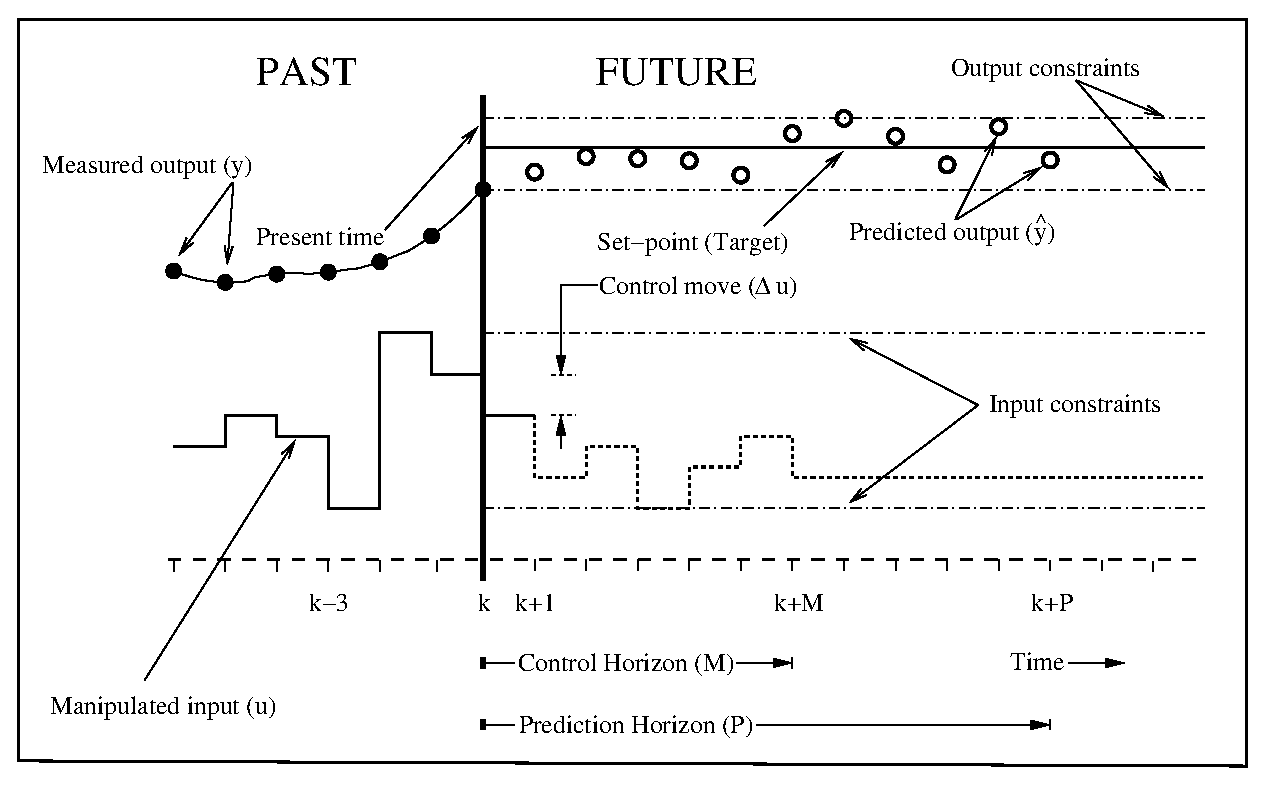
\includegraphics[width=5in]{mpc.eps}
\end{center}
\renewcommand{\baselinestretch}{1}
\small\normalsize
\begin{quote}
\caption[Figure with caption indented]{This figure caption is indented and single-spaced.  Comparison between the experimental measurements \cite{hart1} (black), the random initial condition NLSE model excluding phase noise (dashed curves) and the stochastic phase noise NLSE model (solid curves) showing the first- and second-order sideband evolution as a function of fiber length for P$_{0} = 5.5$\,W, $\Omega = 366$\,GHz, $\Delta\nu = 0.5$\,GHz, $\gamma = 0.019$\,W$^{-1}$m$^{-1}$, and $\beta^{(2)} = 55$\,ps$^2$/km: dynamical evolution of the: (a) power in the first-order blue-shifted sideband, (b) power in the first-order red-shifted sideband, (c) fluctuations in the first-order blue-shifted sideband, (d) fluctuations in the first-order red-shifted sideband, (e) power in the second-order blue-shifted sideband, (f) power in the second-order red-shifted sideband. \label{fig:fig27}}
\end{quote}
\end{figure}
\renewcommand{\baselinestretch}{2}
\small\normalsize

The first figure is Fig.\ref{fig:fig27}.   Please note that the figure label should be placed inside the figure caption.
\newpage

The next figure is placed landscape.  It is Fig.~\ref{fig:mpc}.

\begin{landscape}
\renewcommand{\baselinestretch}{1}
\small\normalsize
\begin{quote}
\begin{figure}
\begin{center}
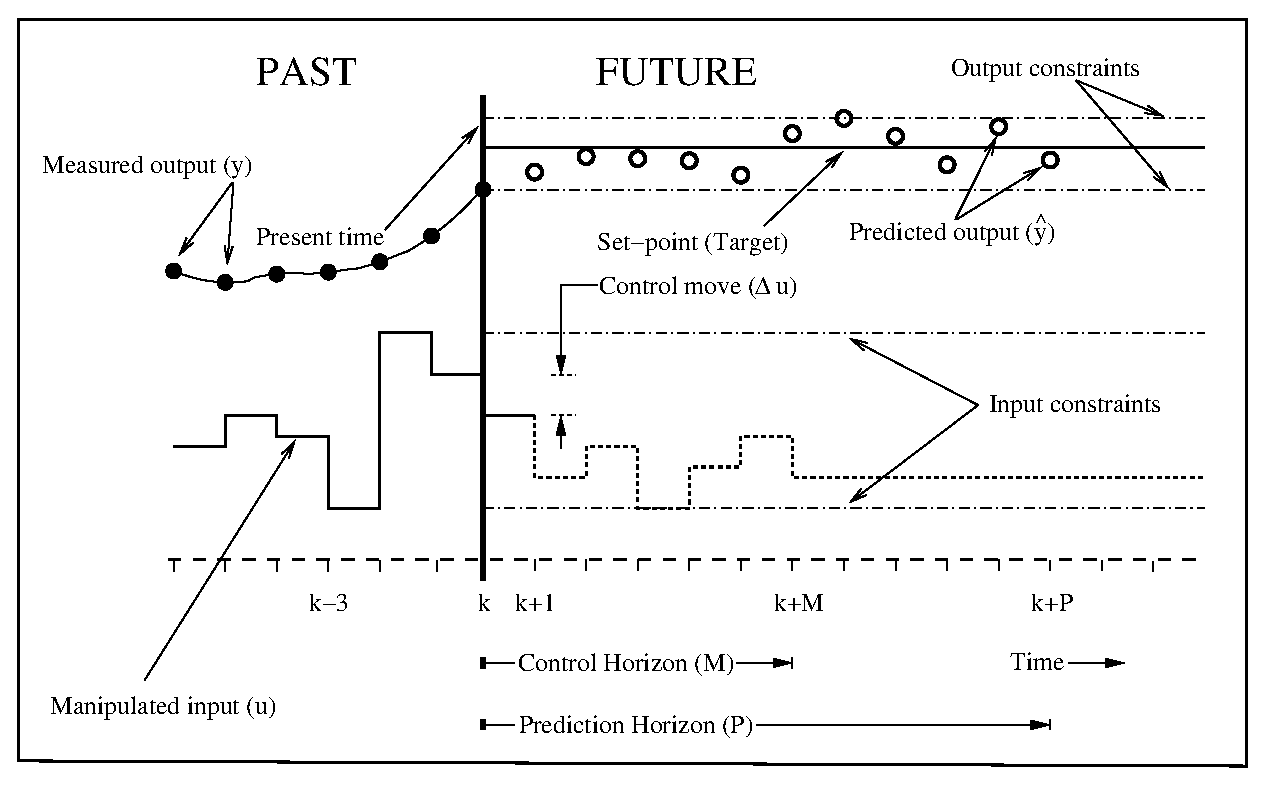
\includegraphics[width=8.2in]{mpc.eps}
\end{center}
\caption{Schematic illustrating receding horizon control.
\label{fig:mpc} }
\end{figure}
\end{quote}
\renewcommand{\baselinestretch}{2}
\small\normalsize
\end{landscape}

This is a my second figure which was placed landscape.  Although I have used the same figure, I have renamed the label to fig:mpc-1.  The second figure now becomes Figure~\ref{fig:mpc-1}.
\begin{landscape}
\renewcommand{\baselinestretch}{1}
\small\normalsize
\begin{quote}
\begin{figure}
\begin{center}
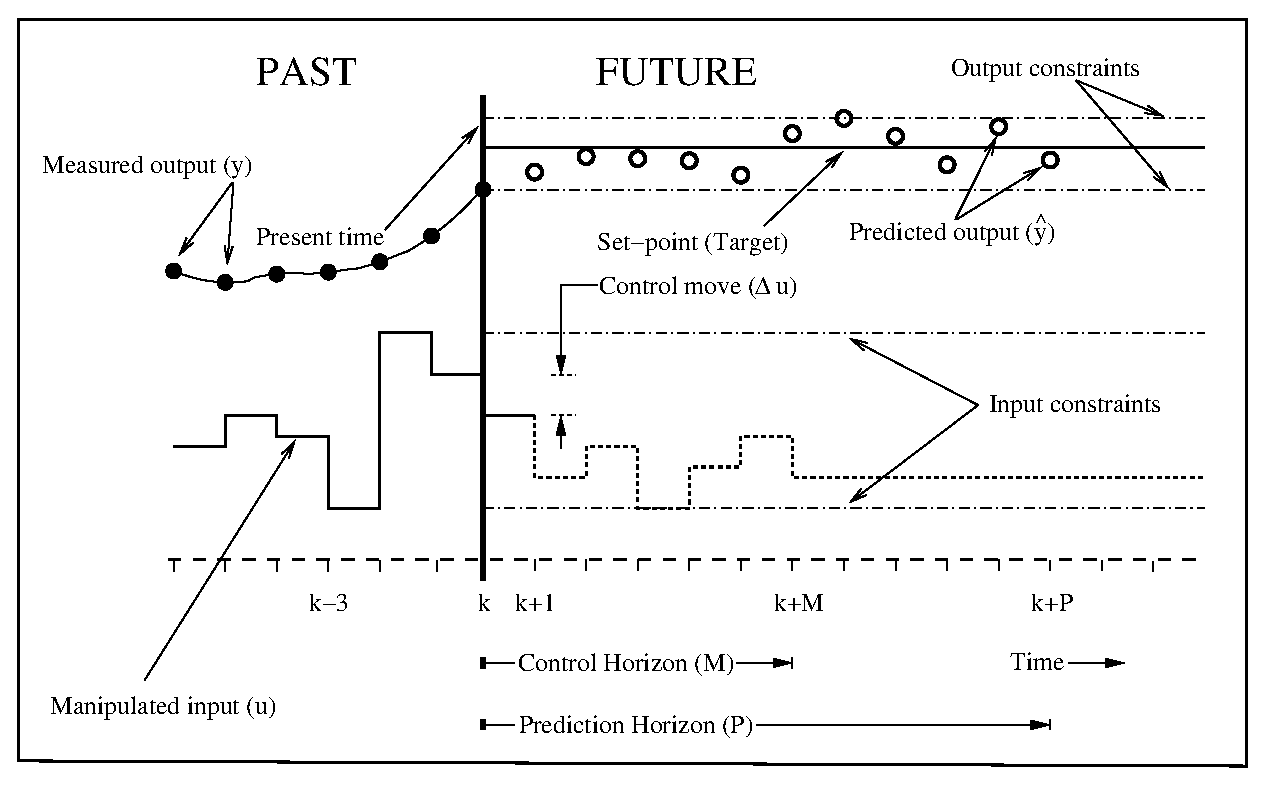
\includegraphics[width=8.2in]{mpc.eps}
\end{center}
\caption[Figure placed landscape on page]{Schematic illustrating receding horizon control. \label{fig:mpc-1}}
\end{figure}
\end{quote}
\renewcommand{\baselinestretch}{2}
\small\normalsize
\end{landscape}

\subsection{Numbering Figures}

If you wish your figures to be numbered 1-100 without any reference to the chapter (e.g., Figure 1.1, 2.1, etc.), change the first line of your mainthesis.tex file to read \begin{verbatim}"\documentclass[12pt]{thesis-2}".\end{verbatim}

\subsubsection{This is a Subsubsection}

This is my first subsubsection in Chapter 1.


\section[Short Titles]{Short Titles in the Table of Contents, List of Figures, or List of Tables}

The Table of Contents, List of Figures, or List of Tables usually show the entire title of a section, subsection, etc. or table, or the entire caption of a figure.  If you put a short title in square brackets after \begin{verbatim} \section, \table, or \figure, \end{verbatim} the short title will show in your Table of Contents or lists.

\renewcommand{\baselinestretch}{1}
\small\normalsize

\begin{verbatim}
\section[Short Title]{Title of Section}
\subsection[Short Title]{Title of Subsection}
\end{verbatim}

or when using a caption in a figure or table
\begin{verbatim}
\caption[Short Caption]{Full text of the caption.}
\end{verbatim}

\renewcommand{\baselinestretch}{2}
\small\normalsize


\section{Figures on Text Page}

Normally figures in the thesis are placed on a page by themselves.  The following figure is placed on the page with text before and after the figure by adding [!!h] after \begin{verbatim} \begin{figure}[!!h] \end{verbatim}.  Please note that the figure label is placed within the caption.

\renewcommand{\baselinestretch}{1}
\large\normalsize

\begin{verbatim}
\begin{figure}[!!h]
 \begin{center}
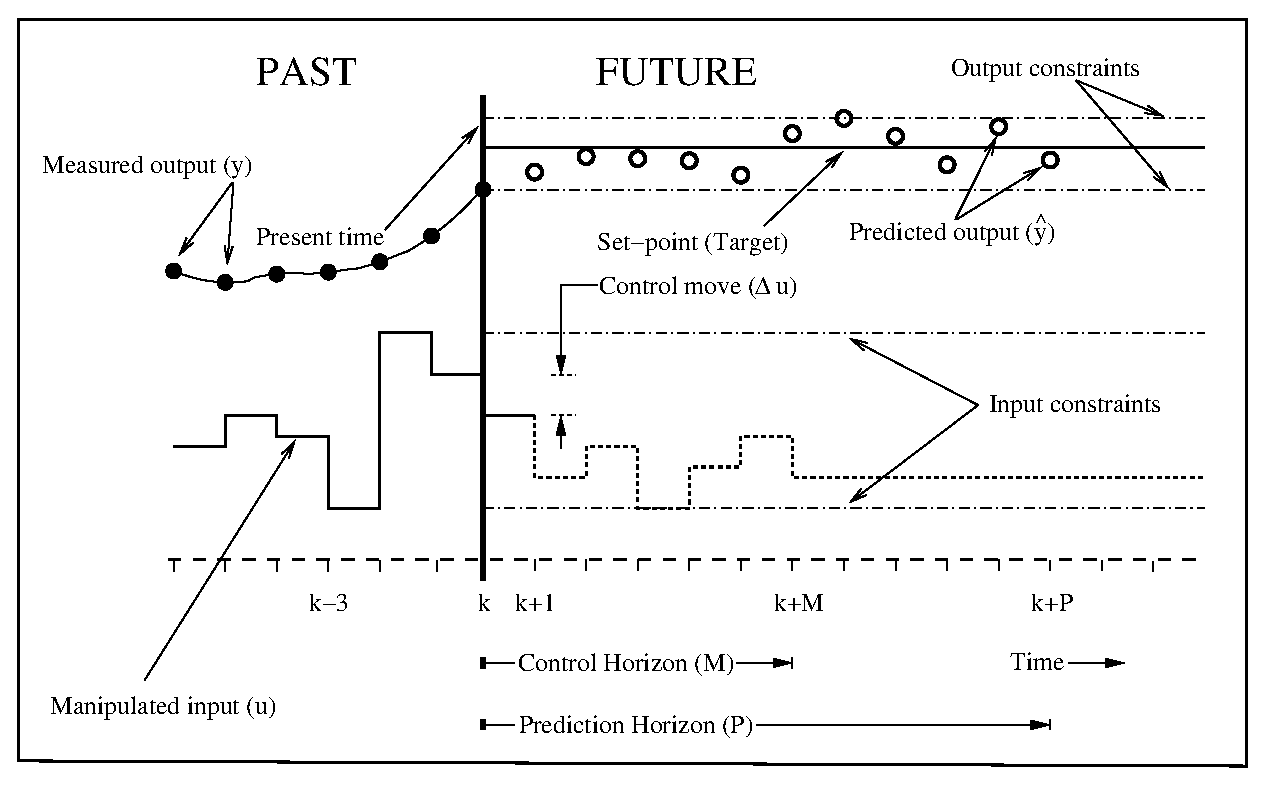
\includegraphics[width=5in]{mpc.eps}
\end{center}
\caption[Short title]{Schematic illustrating receding horizon control.
\label{fig:mpc-2}}
\end{figure}
\end{verbatim}

\begin{figure}[!!h]
 \begin{center}
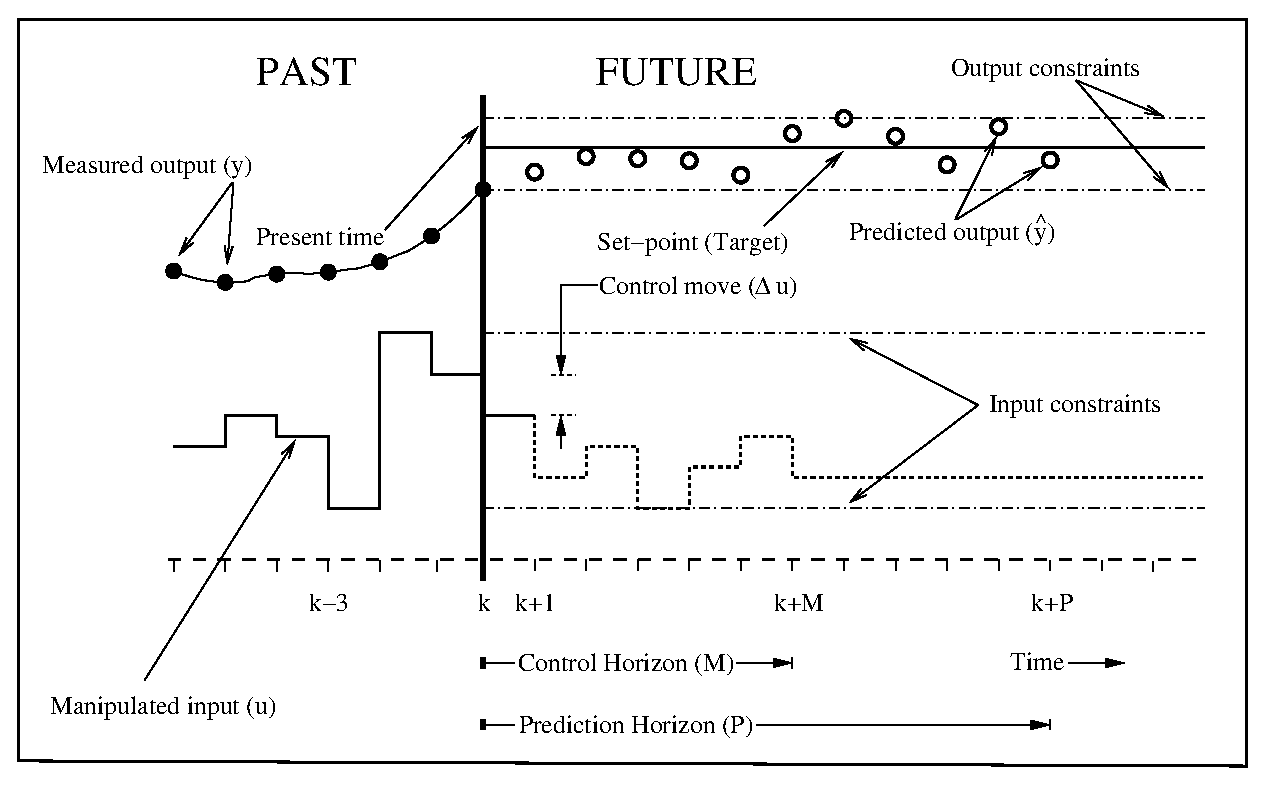
\includegraphics[width=5in]{mpc.eps}
\end{center}
\caption{Schematic illustrating receding horizon control. \label{fig:mpc-2}}
\end{figure}

\renewcommand{\baselinestretch}{2}
\large\normalsize

This does not necessarily mean that the text before and after the figure will be exactly what you want.  Remember Latex will place the figure where it will fit on the page the best.   The previous figure is Figs.~\ref{fig:mpc-2}.

\section{Wrapping Text around Figure}


\renewcommand{\baselinestretch}{1}
\begin{wrapfigure}{r}{0.4\textwidth}
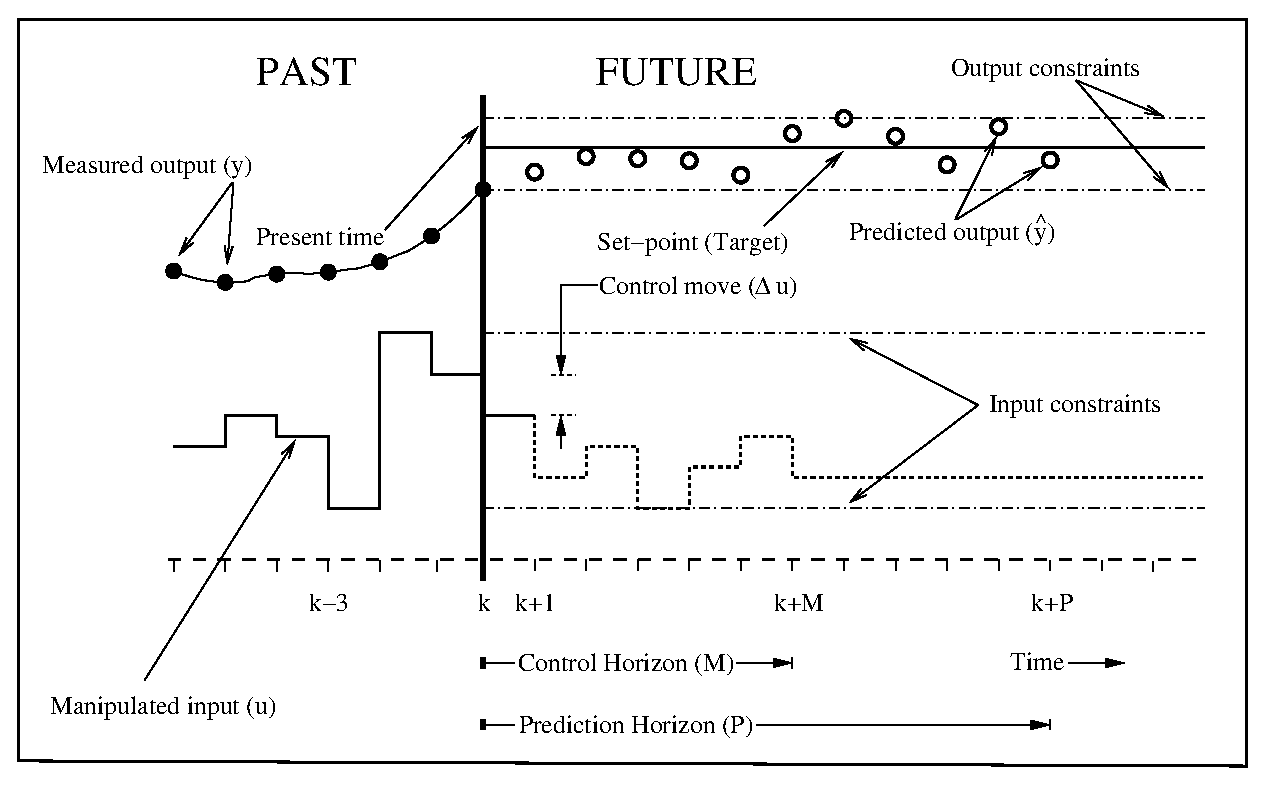
\includegraphics[width=0.4\textwidth]{mpc.eps}
\caption{ Text wrap around figure. \label{fig:test}}
\end{wrapfigure}

\renewcommand{\baselinestretch}{2}
\large\normalsize

By way of summary, at the end of the activity, I reminded the class of what we'd done:  by considering relatively nearby galaxies whose distance we had measured by some other means, we were able to establish a relationship locally between redshift and distance.
By way of summary, at the end of the activity, I reminded the class of what we'd done:  by considering relatively nearby galaxies whose distance we had measured by some other means, we were able to establish a relationship locally between redshift and distance.
By way of summary, at the end of the activity, I reminded the class of what we'd done:  by considering relatively nearby galaxies whose distance we had measured by some other means, we were able to establish a relationship locally between redshift and distance.
By way of summary, at the end of the activity, I reminded the class of what we'd done:  by considering relatively nearby galaxies whose distance we had measured by some other means, we were able to establish a relationship locally between redshift and distance.  See Fig.~\ref{fig:test}.


\section{LaTeX -- A Typesetting Program}

A 13-page explanation of some of the features of LaTeX can be downloaded from http://www.jgsee.kmutt.ac.th/exell/General/LaTeX.html.


\section{Using Bibtex}

Using Bibtex with Latex documents is not difficult.  The bulk of the work is organizing your bibtex file, which is a data base compiled by you of the articles, books, etc. which you use in the bibliographies or reference sections of your publications.

I have linked several files to this webpage, which will be helpful when you are using Bibtex.  These files can be downloaded from \newline
http://www.ireap.umd.edu/ireap/theses/bibtex.  Please read the file "BibtexInstructions.pdf".  The first two pages explain how to set up and run Bibtex; the remaining pages were taken from a published article and show how the references were cited in the .tex file.   The files BibtexInstructions.tex, Galactic.bib, Dottie.bib are the original .tex files used for BibtexInstructions.pdf.  The file BibtexSamples.tex contains examples of the information needed for the various publications you wish to reference (e.g., articles in refereed journals, books, unpublished articles, conference proceedings, etc.).

If you have questions concerning Bibtex, please contact me at 301-405-4955 or dbrosius at umd.edu.

\section{Using Natbib}

Another option of citing references in the bibliography is using
Natbib instead of Bibtex.  You must still create a bibtex file, as
noted above.  The command "backslash cite" cannot be used with
natbib; instead "backslash citet" and "backslash citep" must be
used. "backslash citet" is used to show references in the text
(e.g., Eq.\ 8 in Reiser,1996 shows ...); "backslash citep" is used
in the parenthetical (e.g., Eq.\ 8 (Reiser, 1996) shows ...).

\begin{verbatim}
Add in preamble -- \usepackage[option]{natbib}  --  A list of
options to be used with Natbib can be found at
"http://merkel.zoneo.net/Latex/natbib.php".

Add at bottom of mainthesis.tex file --
\bibliography{name of your bibtex file}
\bibliographystyle{plainnat, abbrnat, or unsrtnat} (I usually use
unsrtnat)

\end{verbatim}

Typesetting:   pdflatex, Bib, pdflatex, pdflatex

I use MikTex with WinEdt.

The reference sheet for natbib usage can be found at \newline "http://merkel.zoneo.net/Latex/natbib.php".

\section{APS Physical Review Style and Notation Guide}

The following style guide may be downloaded from The American Physical Society at http://forms.aps.org/author/styleguide.pdf:  Physical Review Style and Notation Guide, published by The American Physical Society, compiled and edited by Anne Waldron, Peggy Judd, and Valerie Miller, February 1993.  It may be old, but it is very useful.



%%Chapter 3

\renewcommand{\thechapter}{3}

\newcommand{\swave}[0]{$\it{s}$-wave}
\newcommand{\pwave}[0]{$\it{p}$-wave}
\newcommand{\K}{$^{40}\rm{K}$}
\newcommand{\Rb}{$^{87}\rm{Rb}$}
\newcommand{\us}{$\rm{\mu s}$}
\newcommand{\mT}{$\rm{mT}$}
\newcommand{\ez}{$\bf{\mathit{e}_z}$}
\newcommand{\ex}{$\bf{\mathit{e}_x}$}
\newcommand{\um}{$\rm{\mu m}$}
\renewcommand{\thefootnote}{\arabic{footnote}}



\chapter{Direct measurement of a Feshbach resonance in \K{} via observation of \textit{s}-wave scattering}

\section{Introduction}
Feshbach resonances are widely used for tuning the interaction strength in ultracold atomic gases. They have been particularly instrumental in the study of interactions and interaction-dependent processes in cold Fermi gases. In contrast to atomic Bose-Einstein condensates (BECs), where even weak interactions play a crucial role, for example giving rise to their characteristic Thomas-Fermi density profiles \cite{KetterleBEC},  interractions must compete with the Fermi energy before becoming relevant. Practically speaking, the density of Fermi clouds is typically $\sim$1000 times less than that of BECs \footnote{This is not the case for recently realized erbium and dysprosium DFGs \cite{Aikawa14,Lu12}, where strong dipolar interactions are present.}, making it necessary to enhance the strength of interactions in order to observe significant interaction effects\cite{KetterleDFG}. The tunability of interactions provided by Feshbach resonances has allowed for creation of molecular Bose-Einstein condensates from Fermi gases \cite{Greiner03,Zwierlein03, Jochim03} as well as observation of the phase transition from the Bardeen-Cooper-Schrieffer (BCS) superconduting regime to the BEC regime at sufficiently low temperatures \cite{Bartenstein04, Bourdel04, Zwierlein04, Regal04}.
\par A Feshbach resonance occurs when a diatomic molecular state energetically approaches the two-atom continuum \cite{Chin10, Timmermans99}. In experiment, the relative energy of the free atomic states in two hyperfine sublevels and the molecular state is defined by a bias magnetic field. Consequently, the Feshbach resonance can be accessed by changing the bias field. In the simple case where there are no inelastic two-body channels, such as for the \K{} resonance discussed in this work, the effect of the resonance on the scattering length between two free atoms is \cite{Chin10}
\begin{equation}
a(B)=a_{\rm{bg}}\left(1-\frac{\Delta}{B-B_0}\right),
\label{feshbachEq}
\end{equation}
where $a_{\rm{bg}}$ is the background scattering length, $\Delta$ is the width of the resonance, and $B_0$ is the field value at which the resonance occurs. The scattering length diverges at the resonance.
\par  The exact value of the resonant field $B_0$ is difficult to calculate analytically and is commonly computed via numerical models based on experimental input parameters \cite{Tiesinga93, Lysebo09, Gao11} or determined experimentally \cite{Inouye98, Cornish00}. Many experimental techniques have been used to characterize Feshbach resonances, including the observation of atom loss due to three-body inelastic scattering, measurement of re-thermalization timescales, and anisotropic expansion of the cloud upon release from a confining potential, all of which infer the elastic scattering cross section from collective behavior of the cloud \cite{Regal03,OHara02,Monroe93}.
\par Here we used direct scattering as a primary probe of the location and width of a Feshbach resonance. We collided pairs of ultra-cold Fermi gases and directly imaged the resulting \swave{} scattered atoms as a function of magnetic field strength. This allowed us to observe the enhancement in scattering without relying on proxy effects. We measured the fraction of atoms scattered during the collision, and from this fraction deduced the resonant magnetic field  and the width of the resonance.
%A similar technique has been used to characterize impurity scattering in BECs \cite{Chikkatur00}.
%\par The techniques developed in this experiment for observing Fermion scattering can be extended to engineering higher order partial wave interactions, as has been done for bosons \cite{Williams2012}.

In our dilute DFGs, even with the resonant enhancement of the scattering cross section, only a small fraction of the atoms scattered as the clouds passed through each other. This made direct detection of scattered atoms difficult due to detection uncertainty that disproportionately affected regions of low atomic density. To optimize the signal-to-noise ratio (SNR) for low atom numbers, we absorption imaged with fairly long, high-intensity pulses --- a non-standard regime, where the atoms acquired a velocity during imaging and the resulting Doppler-shift was non-negligible.  Simulation of the absorption imaging process was necessary for an accurate interpretation of these images. Using the simulation-corrected images, we extracted the fraction of atoms scattered in our collision experiment.

This paper is divided into two parts. In the first, we study absorption imaging in the presence of a significant time-dependent Doppler shift and show how we use our results to interpret data. In the second, we describe our \swave{} scattering experiment and extract a measure of the location and width of the Feshbach resonance in \K{}.

\section{Experimental setup}
In this section we describe our Fermi scattering experiment. We collided two counter-propagating \K{} clouds and observed the resulting \swave{} halo of scattered atoms.  We measured the dependence of the scattered atomic fraction on the bias magnetic field in the vicinity of the Feshbach resonance. We used this data to extract the location of the magnetic fields resonance of 20.206(15) \mT{} and a width of 1.0(5) \mT{}, similar to the accepted values of 20.210(7) \mT{} and 0.78(6) \mT{} \cite{Regal04}.

We prepared clouds of cold \K{} atoms in a hybrid \K{} and \Rb{} apparatus, previously described in \cite{Williams13, Lin09, KarinaThesis}. We used a Zeeman slower to slow both species before capturing in a magneto-optical trap (MOT). After 7 s seconds of MOT loading \K{} followed by 1.5 s of loading both \K{} and \Rb{}, we cooled both species in optical molasses for 2 ms. We optically pumped both species into their maximally stretched magnetically trappable states, $\ket{F=9/2, m_F=9/2}$ for \K{} and $\ket{F=2,m_F=2}$ for \Rb{}. Both species were then loaded into a quadrupole magnetic trap with a $\approx$ 7.68 mT/cm gradient along \ez, and cooled evaporatively via forced RF evaporation, sweeping the RF frequency from 18 MHz to 2 MHz in 10 s. The magnetic trap was plugged by a $\lambda =$ 532 nm beam, tightly focused to $\approx$ 30 \um{} and $\approx$ 5 W in power, providing a repulsive potential around the zero field point to prevent Majorana losses. Since the \K{} atoms were spin polarized and therefore only interacted by the strongly suppressed \pwave{} interactions, they re-thermalized only due to sympathetic cooling with \Rb{} atoms.

We then loaded the atoms into a crossed optical dipole trap, provided by a 1064 nm fiber laser, and continued evaporative cooling by slowly ramping down the dipole trap to trap frequencies of $(\omega_x,\omega_y,\omega_z)/2\pi =(39, 42, 124)$ Hz in the three spatial directions, while also turning off the quadrupole field. We then used adiabatic rapid passage (ARP) to transfer the \Rb{} atoms from the $\ket{F=2, m_F=2}$ state to the  $\ket{F=1, m_F=-1}$ absolute ground state via 6.8556 GHz microwave coupling (20.02 MHz from the zero field resonance) followed by a magnetic field sweep from -0.469 mT to -0.486 mT in 50 ms. This state was chosen to minimize spin changing collisions with \K{} atoms during any further evaporation \cite{BestThesis}.  We then briefly applied an on-resonant probe laser, ejecting any remaining \Rb{} atoms in the $F=2$ manifold from the trap. We again used ARP to transfer the \K{} atoms into the $\ket{F=9/2,m_F=-9/2}$ state by using a 3.3 MHz rf field and sweeping the bias magnetic field from -0.518 mT to -0.601 mT in 150 ms.

Following the state transfer, we had two versions of the protocol \--- one for approaching the Feshbach resonance from higher fields and one for approaching it from lower fields. For approaching the resonance from lower fields, we proceeded by ramping the bias magnetic field to 19.05 mT, turning on a 42.42 MHz RF field, and then sinusoidally modulating the bias field at 125 Hz for 0.5 s, with a 0.14 mT amplitude, decohering the \K{} state into an equal mixture of $\ket{F=9/2,m_F=-9/2}$ and $\ket{F=9/2,m_F=-7/2}$. For approaching the resonance from higher fields, the same was done at a bias field of 21.71 mT and an RF frequency of 112.3 MHz. The depolarization allowed the \K{} atoms to interact and re-thermalize, allowing us to further evaporate in the dipole trap \cite{DeMarco99}. Since \Rb{} is heavier than \K{}, we were able to evaporate the \K{} atoms past the point where \Rb{} atoms were no longer suspended against gravity and had been completely removed.  These hyperfine states of \K{} were then used to study their Feshbach resonance.
\par After evaporation, we ramped the bias field in a two-step fashion to the desired value $B$ near the Feshbach resonance. We approached the field using a large pair of  coils in Helmholtz configuration (0.19 mT/A) to bring the magnetic field to a setpoint 0.59 \mT{} away from $B$,  $B-0.59$ \mT{} when approaching from below and $B+0.59$  \mT{} from above. We held the atoms at this field for 100 $\rm{ms}$ to allow the eddy currents induced by the large coils to settle, and then used a lower inductance (0.017 mT/A) set of Helmholtz coils to quickly change the field the remaining 0.59 \mT{}. This allowed us to study the resonance from both sides without the added losses associated with going through the resonance \cite{Chin10}.

Once at the intended bias field, we split the cloud into two spatially overlapping components with opposing momenta  and observed scattering as they moved through each other and separated. These counterpropagating components were created using an  8$E_{\rm{L}}$ deep near resonant ($\lambda_{\rm{L}}$=766.704 nm) 1-d retro-reflected optical lattice, where $E_{\rm{L}}=\hbar^2 k_{\rm{L}}^2/2m_{\rm{K}}$ is the lattice recoil energy and $\hbar k_{\rm{L}}=2\pi \hbar/ \lambda$ is the recoil momentum. We rapidly pulsed this lattice on and off with a double-pulse protocol \cite{Wu05, Edwards10}. The pulse sequence was optimized to transfer most of the atoms into the $\pm 2 \hbar k_{\rm{L}}$ momentum states. Since the initial Fermi gas had a wide momentum spread (in contrast to a BEC, which has a very narrow momentum spread), and the lattice pulsing is a momentum dependent process  \cite{Wu05}, not all the atoms were transferred into the target momentum states. We optimized our pulse times to minimize the atoms remaining in the zero momentum state. The optimized pulse times were 23 \us{} for the first pulse, 13 \us{} off interval, and 12 \us{} for the second pulse \cite{Edwards10}.

We then released the atoms from the trap and allowed 1 ms for the two opposite momentum states within the cloud to pass through each other, scattering on the way. For the data taken coming from below the Feshbach resonance, we then simply ramped down the field and imaged the atoms. For the data taken coming from above the Feshbach resonance, we ramped the field back up, retreating through the resonance if it had been crossed and thereby dissociating any molecules that were created, and then quickly ramped the field back down and imaged the atoms. We used a 40 \us{} imaging pulse with $I_0/I_{\rm{sat}}\approx 0.6$ at the center of the probe laser.

The total time-of-flight, the time from the moment the atoms were released from the trap to when they were imaged, was $t_{TOF}=6.8$ $\rm{ms}$. In such an image, the observed atomic position is determined by the initial velocity upon release from the trap, along with the time-of-fligt time $t_{TOF}$. Therefore, this technique measures the momentum and not the position distribution of the atoms.

The magnetic fields produced by our coils in the regime of interest were independently calibrated by rf-spectroscopy. We prepared \K{} atoms in the $\ket{F=9/2, m_F=-9/2}$ state and illuminated them with and rf-field with some frequency $\nu_{rf}$. We then ramped our high-inductance coils to variable set points, followed by an adiabatic 250\us{} ramp of 2.84 mT in the lower inductance coils. We then used Stern-Gerlach and observed the fractional population in the $\ket{F=9/2, m_F=-9/2}$  and $\ket{F=9/2, m_F=-7/2}$ states as a function of the high-inductance coil current. We fit the fractional population curve to a Gaussian, and considered the center of the fit to be on-resonant, with an uncertainty given by the Gaussian width. We used the Breit-Rabi formula to determine the resonant field value at $\nu_{rf}$. We did this for 5 different rf frequencies, and acquired a field calibration with an uncertainty of 0.3 mT, which was included in the listed uncertainty on the center field of the Feshbach resonance.


\section{Methods}

We first processed each image by comparing the obsereved $OD$s to simulations taking into account the recoil induced detuning as described in Sec. \ref{sec:2}. An example of images before and after processing are shown in Fig. \ref{fig:SampleCorrection}.  To improve the signal and mitigate our shot to shot number fluctuations, we took 15 nominally identical images for each data point.
\begin{figure}
	\subfigure[]{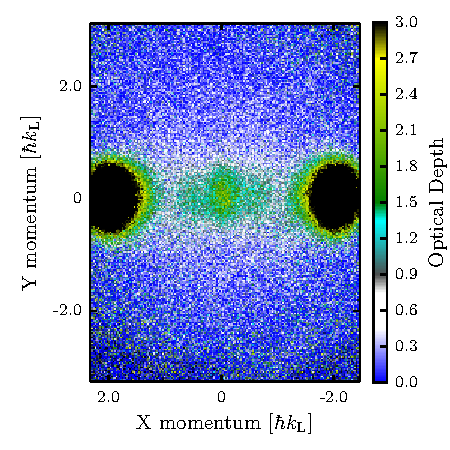
\includegraphics{Chapter3 Figures/figure10a.pdf}}
	\subfigure[]{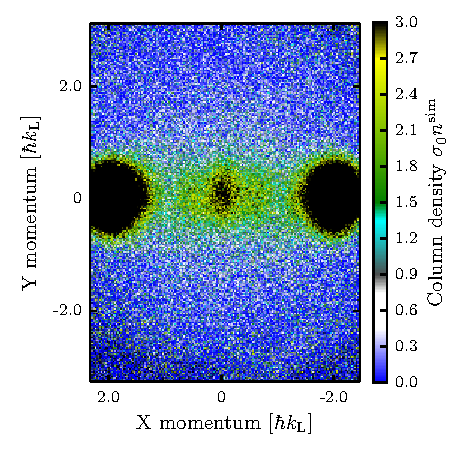
\includegraphics{Chapter3 Figures/figure10b.pdf}}
\caption{An example of our absorption image after 6.8 ms TOF. The 1-D lattice imparts momentum along \ex{}. The two large clouds on the left and right are the atoms in the $\pm 2 k_{\rm{L}}$ momentum orders that passed through each other unscattered. The smaller cloud in the center is the atoms that remained in the lowest band of the lattice after pulsing, and thus obtained no momentum. The thin spread of atoms around these clouds is the atoms that underwent scattering.   This image was taken coming from below the Feshbach resonance at 20.07  \mT{}. (a) Raw optical depth, (b) atomic column density obtained by comparing to simulated $OD$s, $\sigma_0 n^{\rm{sim}}$ }
\label{fig:SampleCorrection}
\end{figure}

We counted the fraction of atoms that experienced a single scattering event for each of the fifteen images at a given bias magnetic field. Single scattering events are easily identified, as two atoms that scatter elastically keep the same amplitude of momentum, but depart along an arbitrary direction. Therefore, an atom traveling at $2 \hbar k_{\rm{L}}$ to the right that collides elastically with an atom traveling at $-2 \hbar k_{\rm{L}}$ to the left will depart with equal and opposite momenta $2 \hbar k_{\rm{L}}$ at an arbitrary angle, and in a time of flight image such atoms will lie in a spherical shell, producing the scattering halo pictured in Fig. \ref{fig:halo}(a).
\begin{figure}
	\subfigure[]{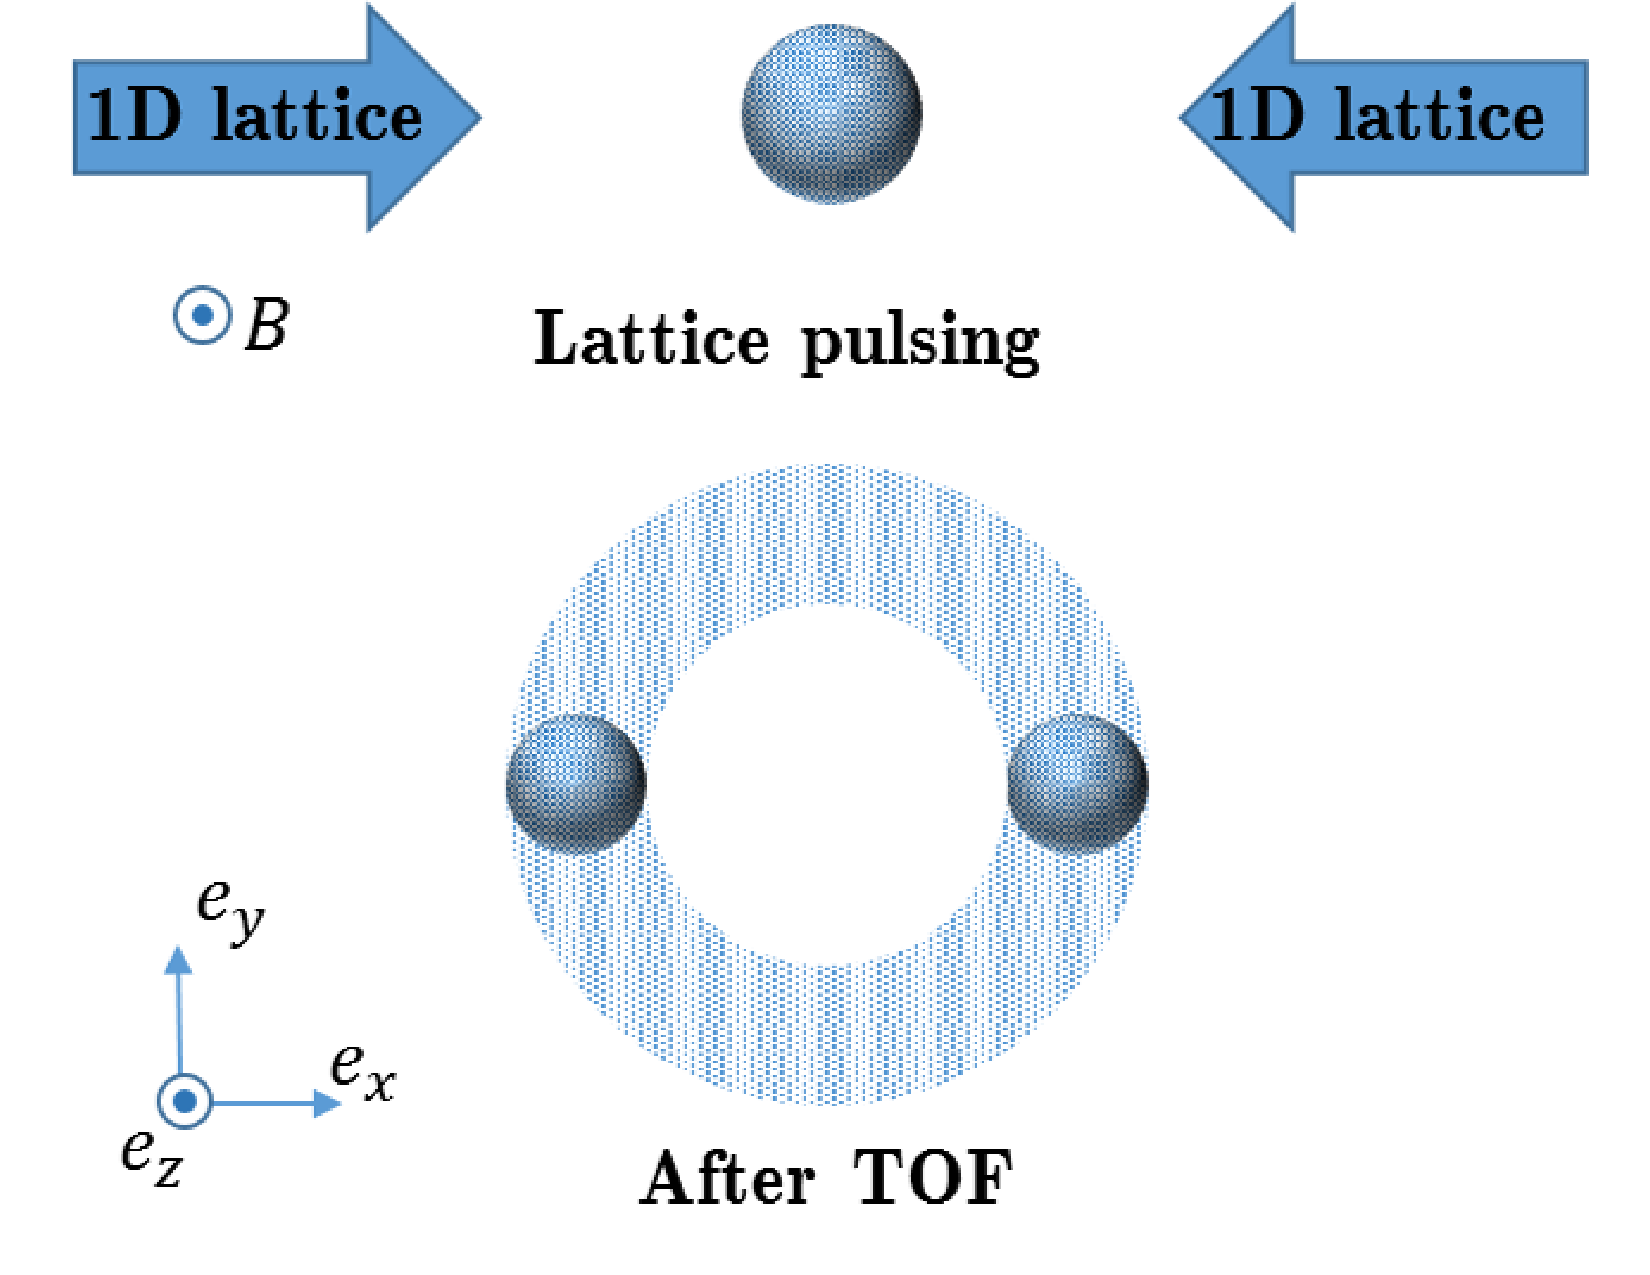
\includegraphics[scale=0.25]{Chapter3 Figures/Picture12.pdf}}
	\subfigure[]{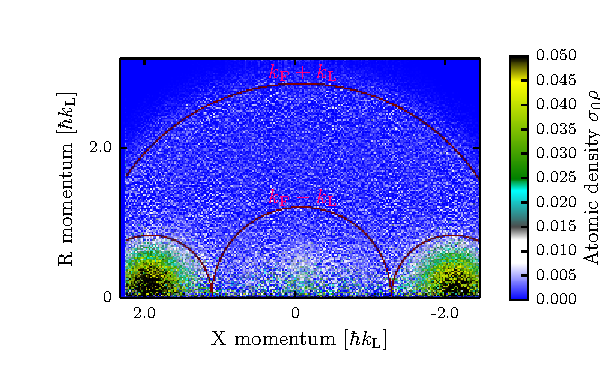
\includegraphics{Chapter3 Figures/figure12b.pdf}}
\caption{(a) Our experimental setup. After time of flight, the two clouds traveling along $\pm \hat{e}_x$ directions have separated and the atoms that underwent a single scattering event were evenly distributed in a scattering halo around the unscattered clouds. The 1-D lattice defined the axis of cylindrical symmetry. (b) Inverse Abel transformed image. The atoms within the Fermi momentum $k_F$ of each unscattered cloud center are in the unscattered region and counted towards the total unscattered number. The atoms outside the radius $ k_{\rm{L}}-k_{\rm{F}}$ but inside $k_{\rm{L}}+k_{\rm{F}}$ but outside the unscattered region are counted towards the number of single scattered atoms.   }
\label{fig:halo}
\end{figure}

Absorption images captured the integrated column density along \ez{}, a projected 2D atomic distribution. To extract the radial dependence of the 3D distribution from the 2D image, we performed a standard inverse Abel transform. The inverse Abel transform assumes cylindrical symmetry, which was present in our case, with the axis of symmetry along \ex{}, defined by the lattice. We neglect the initial asymmetry of the trap, as during time-of-flight the atoms travel far beyond the initial extent of the cloud  $(r_x,r_y,r_z)\approx$ (45,48,15) \um{}, while the cloud width after TOF is $\approx$ 82 \um in each direction. We thus obtained the atomic distribution $\rho(r,\theta)$ as a function of $r$, the radial distance from the scattering center, and $\theta$, the angle between $r$ and symmetry axis \ex{}, integrated over $\phi$, the azimuthal angle around the $x$ axis.

We then extracted the number of scattered atoms $N_{\rm{scat}}$ as a fraction of the total atom number $N_{\rm{tot}}$ for each image, as shown in Fig. \ref{fig:halo}(b). The unscattered atom number was the number of atoms in the two unscattered clouds. The number of atoms that underwent a single scattering event was the number of atoms outside the Fermi radius of the unscattered clouds, but inside the arc created by rotating the Fermi momentum $k_{\rm{F}}$ around the original center of the cloud (red arcs in Fig. \ref{fig:halo}(b)). For both the scattered and unscattered numbers, we accounted for atoms that fell outside the field of view of our camera by multiplying the counted atom number by a factor of the total area as defined by the radii divided by the visible area on the camera. The atoms in the center region were not counted as they were originally in the zero momentum state and could not contribute to the scattering halo under study.

We fit the fraction of scattered atoms versus the total atom number for each of the 15 images taken at the same bias magnetic field to a line constrained to be zero at zero. The slope of this fit was taken to be the value of $N_{\rm{scat}}/N_{\rm{tot}}^2$ at that bias magnetic field, and the variance of the fit gave the uncertainty on that data point. This uncertainty reflected our shot to shot number fluctuations, which produced variable atomic densities and thus influence the scattered fraction. 

We then deduced the resonant field value $B_0$ and width of the resonance  $\Delta$, the parameters in Eq. (\ref{feshbachEq}).  Since we were in the low energy regime (the atomic momentum was much smaller than the momentum set by the van der Waals length $k_{\rm{L}}+k_{\rm{F}}\ll1/l_{\rm{vdW}}$, and we were well below the p-wave threshold temperature \cite{DeMarco99}), the scattering cross-section was given by $\sigma=4\pi a^2$.

The scattering cross-section $\sigma$ gives the probability $P_{\rm{scat}}=\sigma N/A$ that a single particle will scatter when incident on a cloud of atoms with a surface density of $N/A$, where $A$ is the cross-sectional area of the cloud and $N$ is the number of atoms in the cloud. In our case, each half of the initial cloud, with atoms number $N_{\rm{tot}}/2$, is incident on the other half. Thus, the number of expected scattering events is $N_{\rm{scat}}= (N_{\rm{tot}}/2) \sigma  (N_{\rm{tot}}/2)=\sigma N_{\rm{tot}}^2/4A$. Assuming $A$ is constant for all our data, we can define a fit parameter $b_0=4\pi a_{\rm{bg}}^2/4A$, where $a_{\rm{bg}}$ is the background scattering length. We can thus adapt Eq. (\ref{feshbachEq}) to obtain the fit function
\begin{equation}
\frac{N_{\rm{scat}}}{N_{\rm{tot}}^2}=b_0\left(1-\frac{\Delta}{B-B_0}\right)^2 + C.
\label{eq:fit}
\end{equation}
We found that our imaging noise skewed towards the positive, giving rise to a small background offset. We accounted for this in our fit by including a constant offset parameter $C$.


\section{Results}
Our final data is presented in Fig. \ref{fig:fittedFractions}. The red curve depicts a best fit of the model given in Eq. (\ref{eq:fit}). The fit parameters we extracted were $\Delta = 1(5)$  \mT{}, $B_0 = 20.206(15)$  \mT{}, $b_0 = 5(3)\times 10^{-3}$ and $C=8(1)\times 10^{-4}$. To obtain the fit, we used data taken by approaching the resonance from above for points above where we expected the resonance to be and data taken approaching the resonance from below for points below. We also excluded from the fit data points very near the resonance, as there the assumption $\sigma\rho\ll1$, where $\rho$ is the atom number per unit area, is no longer valid and the problem must be treated hydrodynamically.

The accepted values for the $^{40}K$ s-wave Feshbach resonance for the  $\ket{9/2,-9/2}$ and $\ket{9/2,-7/2}$ states are $B_0=20.210(7)$  \mT{} and $\Delta=0.78(6)$  \mT{} \cite{Regal04}, which is in good agreement with our findings. Some potential sources of systematic uncertainty that we did not account for include scattering with atoms that did not receive a momentum kick from the lattice pulsing or the impact of multiple scattering events.
\begin{figure}
	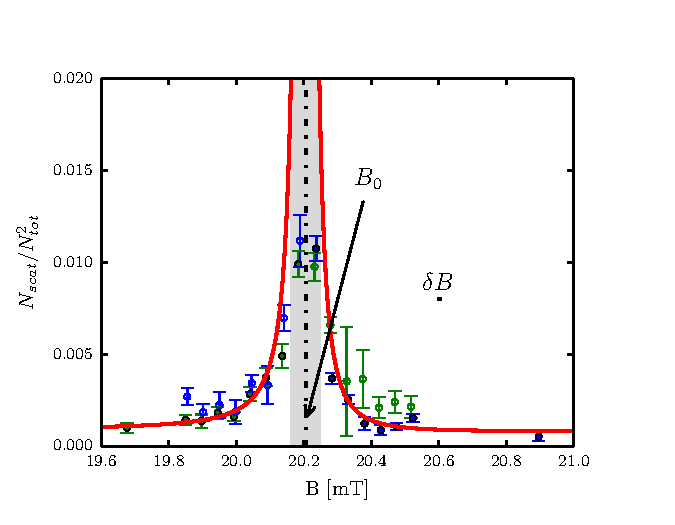
\includegraphics{Chapter3 Figures/figure11.pdf}
\caption{Normalized scattered population plotted versus bias field $B$. Green dots represent data taken coming from below the resonance, and blue dots represent the data taken coming from above the resonance. The red curve depicts the best fit, where data coming from above the resonance was used above the resonance and data coming from below the resonance was used below the resonance to create the fit; the unused data points are indicated by hollow dots. The regime where the scattering length is likely large enough for the atoms to behave hydrodynamically is shaded in gray, and data points in that area were also excluded from the fit. Resonant field value $B_0$ as found in this work and our systematic uncertainty in the bias magnetic field $\delta B_0$ are indicated.    }
\label{fig:fittedFractions}
\end{figure}
\section{Conclusion}
We studied the effects of recoil-induced detuning effects on absorption images and found an optimal imaging time of $\approx40$ \us{} for \K{} atoms for noise minimization after corrections. We use these results to observe s-wave scattering halos of the Fermi gas around the $\approx 20.2$ \mT{} Feshbach resonance and directly verified the resonance location and width. Our analysis can be used in any absorption imaging application where SNR optimization is critical.


%\titleformat{\chapter}
%{\normalfont\large}{Appendix \thechapter:}{1em}{}
\doublespacing
\normalsize
\setcounter{page}{1}
\pagenumbering{arabic}


%\renewcommand{\thechapter}{3}

\chapter{Ultracold Gases and the RbK apparatus}\label{chap:Intro}
In this chapter we intoduce the basics of ultracold quantum gases. When cooled to extremely low temperatures, bosonic atoms form Bose Einstein condensates, described in sec. \ref{sec:BECintro}. Fermionic atoms do not undergo a phase transition, but gradually become degenerate, forming what's known as a degenrate Fermi Gas, described in sec. \ref{sec:DFGintro}. We then give a basic overview of the rubidium-potassium (RbK) apparatus at NIST, on which the work described in this thesis was done, in sec. \ref{sec:RbK}. We detail some of the changes that have been made to the apparatus since it was last documented.  

\section{Bose-Einstein condensation}\label{sec:BECintro}
In this section, we give some basic background on Bose-Einstein condensation, relevant to \Rb{} atoms cooled in our apparatus. 

\subsection{Phase transition of a non-interacting Bose gas}
Bose gases are characterized by the Bose-Einstein distribution giving the number of atoms $n(E_j)$ occupying each energy eigenstate $E_j$ as
\begin{equation}
n(E_j) = \frac{1}{e^{(E_j-\mu)/k_{\rm B}T}-1},
\end{equation}
where  $k_{\rm B}$ is the Boltzmann constant, $T$ is the temperature in Kelvin, and $\mu$ is the chemical potential. Assuming the total atom number $N$ is fixed, the chemical potential $\mu(T,N)$ ensures that the total occupation $\sum_j n(E_j)=N$. 

The Bose distribution leads to Bose-Einstein condensation, the collapse of a macroscopic fraction of the atoms into the ground state. This comes as a direct consequence of the Bose distribution's characteristic $-1$ in the denominator. Consider the occupation number $n(E_j)$. It must remain positive, as a negative occupation number is unphysical. This implies the quantity $e^{(E_j-\mu)/k_{\rm B}T}$ must remain greater than $1$, or $(E_j-\mu)/k_{\rm B}T>0$ for all $E_j$. Therefore, $\mu\leq E_0$, where $E_0$ is the ground state energy. 

Then, for a given temperature $T$, there is a maximum occupation number for each excited state given by $n(E_j) = \frac{1}{e^{E_j/k_{\rm B}T}-1}$. The only energy state whose occupation number is unbounded is the ground state, as $n(E_0)$ tends toward infinity as $\mu$ tends towards $0$. Therefore, as the temperature decreases, the maximum occupation of each excited state decreases until they can no longer support all $N$ of the atoms. The remaining atoms then have no choice but to collapse into the lowest energy level and Bose condense. 

We will show this quantitatively for the case of a 3-D harmonically trapped gas of non-interacting atoms, relavant to the experiments described in this thesis\cite{Ensher1996}. It is convenient to define the fugacity $\zeta=e^{\mu/k_{\rm B}T}$, and re-write the Bose-Einstein distribution for some 
eigenstate $E_j$ as
\begin{equation}
n(E_j) = \frac{\zeta}{e^{E_j/k_{\rm B}T}-\zeta}.
\end{equation}
The harmonic oscillator potential can be written as 
\begin{equation}
V(r) = \frac{1}{2} m (\omega_x^2 x^2 + \omega_y^2 y^2 + \omega_z^2 z^2),
\end{equation}
where $\omega_x$, $\omega_y$ and $\omega_z$ are the angular trapping frequencies along ${\bf e}_x$, ${\bf e}_y$, and ${\bf e}_z$.  The eigenenergies with this potential are
\begin{equation}
E(j_x,j_y,j_z) = (\frac{1}{2} + j_x)\hbar\omega_x +(\frac{1}{2} + j_y)\hbar\omega_y+(\frac{1}{2} + j_z)\hbar\omega_z.
\end{equation}

In order to find $\mu$, we must find $\sum_{j_x,j_y,j_z}n(E(j_x,j_y,j_z))$ and set it equal to $N$. This task is greatly simplified by going to the continuum limit and finding the density of states. To do this, we neglect the zero-point energy (setting $E_0=0$, the effects of the zero-point energy are discussed in \cite{Pethick} section 2.5)  and assume there is on average one state per volume element $\hbar^3 \omega_x \omega_y \omega_z$. Then, the total number of states with energy less than or equal to some value $\epsilon$ is given by the volume of a prism made between points $(j_x,j_y,j_z)=(0,0,0),(\epsilon,0,0),(0,\epsilon,0)$ and $(0,0,\epsilon)$ in units of the volume element:
\begin{equation}
G(\epsilon) = \frac{\epsilon^3}{6\hbar^3\omega_x \omega_y \omega_z}.
\label{eqn:numberOfStates}
\end{equation}
The density of states is given by 
\begin{equation}
g(\epsilon) = \frac{d}{d\epsilon} G(\epsilon) = \frac{\epsilon^2}{3\hbar^3\omega_x \omega_y \omega_z}. 
\label{eqn:densityOfStates}
\end{equation}

Note that the occupation of the ground state is not included in this continuum picture. We can therefore use it only to calculate the total number of atoms in all of the excites states:
\begin{equation}
N_{\rm ex} = \int_0^{\infty} d\epsilon g(\epsilon) n(\epsilon) = \int_0^{\infty} d\epsilon \frac{\epsilon^2}{3\hbar\omega_x \omega_y \omega_z} \frac{\zeta}{e^{\epsilon/k_{\rm B}T}-\zeta} = \frac{(k_{\rm B}T)^3}{\hbar^3\omega_x \omega_y \omega_z}{\rm Li}_3(\zeta),
\label{eqn:excitedPopulation}
\end{equation}
where ${\rm Li}_3(\zeta)$ is the polylogarithm function\footnote{This calculation was done with Wolfram Alpha, not Russian algebra skills}. 
We define the mean trapping frequency $\bar{\omega} = (\omega_x \omega_y \omega_z)^{1/3}$ and the harmonic oscillator energy as $\hbar\bar{\omega}$, with the thermal energy in harmonic oscillator units $\tau = k_{\rm B}T/\hbar\bar{\omega}$, giving
\begin{equation}
N_{\rm ex} = \tau^3 {\rm Li}_3(\zeta).
\end{equation}

Finding the occupation number of the ground state from the Bose-Einstein distribution
\begin{equation}
N_0 = \frac{\zeta}{1-\zeta},
\label{eqn:groundPopulation}
\end{equation}
we can then find the chemical potential, or equivalently the fugacity $\zeta$, to satisfy
\begin{equation}
N = N_0 + N_{\rm ex}.
\end{equation}
This is a transcendental equation that can only be solved numerically. We present an example of the solution in Figure \ref{fig:BoseDistribution}. Here, we have calculated the fractional population in different harmonic oscillator energy levels for three different temperatures, using trapping frequencies $\omega_x=\omega_y=\omega_z=2\pi\times 50$ Hz, and atom number $N=10^6$. For energies above the ground state (dots in the figure), we binned 50 energy levels together, such that each dot represents the total fractional population in 50 adjacent levels. This was obtained by integrating eqn. \ref{eqn:excitedPopulation} from $\epsilon - 25\hbar\bar{\omega}$ to $\epsilon + 25\hbar\bar{\omega}$. The stars represent the fractional population in just the ground state, calculated from eqn. \ref{eqn:groundPopulation}. Note that at temperature $T=255$ nK (red), the ground state population is consistent with a continuous extrapolation from the excited state populations and is almost zero. At lower temperatures, $T=180$ nK (blue) the ground state population is in excess of any reasonable extrapolation from the excited state fractions, and at $T=80$ nK (green) almost all the atoms are in the ground state. 

\begin{figure}
	\includegraphics{"BEC_DFG figures/condensation".pdf}
\caption[Occupation of energy states of a 3-D harmonic oscillator]{Occupation of energy states of a 3-D harmonic oscillator. The trapping frequencies are $\omega_x=\omega_y=\omega_z=2\pi \times 50$ Hz, and the atom number is $N=10^6$. Dots represent the total fractional population in 50 ajacent energy levels, including degeneracies. The stars represent the fractional population in just the ground state.  }
\label{fig:BoseDistribution}
\end{figure}

The onset of Bose-Einstein condensation occurs at a critical temperature $T_c$. This temperature is defined as the temperature at which the occupation number of excited states is equal to the atom number, i.e. when the atoms have occupied all available excited states and any remaining atoms were forced to pile into the ground state. Since the maximal occupation of the excited states will occur at $\mu=0$, the occupation of the excited state is bounded from above by $N_{\rm ex}(\mu=0)$, and the critical temperature is defined by 
\begin{equation}
N=N_{\rm ex}(\mu=0, T=T_c)=\frac{(k_{\rm B}T_c)^3}{\hbar^3 \omega_x \omega_y \omega_z}{\rm Li}_3(\zeta=1).
\end{equation}
Using ${\rm Li}_3(1)\approx1.202$, we obtain for a given atom number and trapping frequencies
\begin{equation}
T_c = \frac{1.202 N}{k_{\rm B}^3}\hbar^3 \omega_x \omega_y \omega_z.
\label{eqn:tc}
\end{equation}
For the parameters in Figure \ref{fig:BoseDistribution}, $T_c = 225$ nK. 

For temperatures below the critical temperature, the condensation fraction $f_c$---the fraction of atoms in the ground state---is directly related to the ratio of the temperature to the critical temperature:
\begin{equation}
f_c=1-\frac{N}{N_{\rm ex}}=1-\frac{(k_{\rm B}T)^3}{\hbar^3 \omega_x \omega_y \omega_z}{\rm Li}_3(\zeta=1)=1-\left(\frac{T}{T_c}\right)^3,
\end{equation}
where in the last step we have plugged in the definition of the critical temperature eqn. \ref{eqn:tc}.

\begin{figure}
	\includegraphics{"BEC_DFG figures/CondensingAtoms".png}
\caption[Time-of-flight images of atoms]{Time-of-flight images of atoms. (a) Above the critical temperature - the atoms are thermally distirbuted. (b) Below the critical temperature - about half of the atoms are condensed in the central peak. (c) Far below the critical temperature - almost all atoms are condensed in the central peak.}
\label{fig:CondensingAtoms}
\end{figure}

Figure \ref{fig:CondensingAtoms} shows the progression towards condensation as the temperature of a cloud of \Rb{} is decreased below $T_c$. The images are obtained via a time-of-flight measurement (see section \ref{sec:timeOfFlight}), where the atoms are allowed to expand freely, mapping the initial momentum to final position, imaged via absorption imaging (see section \ref{sec:absorptionImaging}). The $x$ and $y$ axes represent momentum along $x$ and $y$, while the z axis represents the number of atoms per spatial bin. The $z$ axis momentum is integrated over.  Figure \ref{fig:CondensingAtoms}a shows a cloud above the condensation temperature - the momentum distribution is nearly gaussian, given by the Maxwell-Boltzmann distribution. In  fig. \ref{fig:CondensingAtoms}b, the temperature has been decreased below $T_c$, and about half the atoms have collapsed into the ground state, producing a large peak in atom number around zero momentum. In  fig. \ref{fig:CondensingAtoms}c, the temperature has been decreased even further and almost all the atoms populate the central peak - the distribution is no longer gaussian but a sharp peak around zero momentum. 


\subsection{Interacting Bose gas}

In the previous section, we assumed there weres no interaction between the atoms other than those enforced by statistics. In this section, we will relax this assumption somewhat and describe the condensed atomic state through its characteristic Gross-Pitaevskii equation. 

Since condensation occurs at very low temperatures, and thus very low kinetic energies, we can assume that any scattering processes between the atoms are $\it{s}$-wave and can be described simply by a scattering length $a$ (equivalent to assuming that the characteristic size of the atomic wavefunction, given by the thermal deBroigle wavelength, is large compared to the scale of the interatomic potential). For $^{87}$Rb, relevant to experiments described in this thesis, the scattering length between two atoms in the $F=2$ hyperfine state is $a=95.44(7) a_0$ \cite{Egorov2013}, where $a_0=5.29\times10^{-11}$ m is the Bohr radius. The short-range interaction between two particles can be approximated as a contact interaction with an effective strength $U_0$ as (see \cite{Pethick} section 5.2.1):
\begin{equation}
U(r_1,r_2) = U_0 \delta(r_1-r_2) = \frac{4\pi\hbar^2 a}{m} \delta(r_1-r_2),
\end{equation}
where $m$ is the atomic mass and $\delta$ is the Dirac delta function. The full Hamiltonian of the many-body system is then
\begin{equation}
H=\sum_i \frac{p_i^2}{2m} + V(r_i) + U_0\sum_{i<j}\delta(r_i-r_j),
\end{equation}
where $i$ labels the particles, $p_i$ is the momentum, $r_i$ is the position, and $V$ is the external potential.

We make the mean field approximation by assuming that no interactions between two atoms take them out of the ground state, and hence all atoms can be assumed to be in the same single particle wavefunction, making the overall wavefunction
\begin{equation}
\Psi(r_1,r_2,...r_N)=\prod_i^N \phi(r_i),
\end{equation}
where $\phi$ is the single particle wavefunction. It is convenient to define the wavefunction of the condensed state, $\psi(r) = \sqrt{N}\phi(r)$, making the normalization $N=\int dr |\psi(r)|^2$.

The energy of this wavefunction under the Hamiltonian above is given by
\begin{equation}
E=\int dr\left[ \frac{\hbar^2}{2m}|\nabla\psi(r)|^2 + V(r)|\psi(r)|^2 + \frac{1}{2}U_0|\psi(r)|^4\right].
\end{equation}
Given $N$ particles, there are $N(N-1)/2$ unique pairs of particles that can have a pairwise interactions, approximately equal to $N^2/2$ for large $N$. The $N^2$ is absorbed into the definition of $\psi$, but the factor of $1/2$ remains on the final interaction term. The task of finding the condensate eigenstate reduces to minimizing this energy under the normalization constraint $N=\int dr |\psi(r)|^2$. This can be done by using the method of Lagrange multipliers to minimize $E-\mu N$. Then, we can minimize this quantity by finding the point where the derivative with respect to $\psi$ and $\psi^*$ is zero. Taking the derivative with respect to $\psi^*$ we obtain 
\begin{equation}
-\frac{\hbar^2}{2m} \nabla^2 \psi(r) + V(r)\psi(r) + U_0 |\psi(r)|^2\psi(r) = \mu \psi(r),
\end{equation}
which is the Gross-Pitaevskii equation. This is a non-linear equation that generally needs to be solved numerically.

There is another approximation that can be made in cases where the atomic density is high enough that the interaction energy is significantly larger than the kinetic energy. Then, the kinetic term in the Hamiltonian can be neglected. This is called the Thomas-Fermi approximation. In this approximation, the wavefunction is given simply by
\begin{equation}
|\psi(r)|^2 = \frac{\mu - V(r)}{U_0}.
\end{equation}
Here, the probability density simply takes the shape of the inverted potential in which the atoms are held. In the case of a harmonically trapped BEC, it is shaped like an inverted parabola. The Thomas-Fermi radius, i.e. the extent of the particle wavefunction, is the point where the probability density goes to zero: $\mu - V(r_0) = 0$. For a harmonic trap, along any direction, this is given by $r_0^2 = 2\mu/m\omega^2$. 

\begin{figure}
	\includegraphics{"BEC_DFG figures/InSitu".pdf}
\caption[In situ measurement of a fraction of bose condensed atoms]{In situ measurement of Bose condensed atoms. (a) Absorption image taken of $\approx1\%$ of the cloud. The $x$ and $y$ axes represent $x$ and $y$ position, while color represents the atom number. (b) The blue line represents atom number as a function of position along the $x$ axis, integrated over the $y$ axis. The black dashed line represents the best fit of a Gaussian function to the atomic distribution. The dashed red line represents the best fit of a Thomas-Fermi profile to the atomic distribution.}
\label{fig:InSitu}
\end{figure}

Figure \ref{fig:InSitu}a shows an absorption image of a small fraction of atoms in a BEC in situ (see section \ref{sec:timeOfFlight}), meaning as it is in the trap - without expanding in time-of-flight. The $x$ and $y$ axes represent position, while color represents the atom number. Figure \ref{fig:InSitu}b shows the atom number integrated over the y-axis in blue. The red dashed lines represent the best fit line to a Thomas-Fermi distribution, here an inverted parabola. The black dashed lines represent the best fit of a Gaussian to the atomic distribution. The Thomas-Fermi distribution matches the atomic distribution more closely in the center where the density is high, but the Gaussian distribution does a better job at the tails of the distribution. This is due to the presence of some fraction of uncondensed atoms, which are well approximated by a Maxwell-Boltzmann distribution. 


\section{Degenerate Fermi Gas}\label{sec:DFGintro}
In this section, we give some basic background on degenerate Fermi gases, relevant to \K{} atoms cooled in our apparatus. 

\subsection{Fermi statistics and the onset of degeneracy}
The occupation of different energy levels $E_j$ by Fermions is given by the Fermi-Dirac distribution:
\begin{equation}
n(E_j)= \frac{1}{e^{(E_j-\mu)/k_BT}+1}.
\end{equation}
The difference from the Bose-Einstein distribution is simply the sign of the $1$ in the denominator. This has important implications, however. First, since $e^x$ varies between $0$ and $\infty$, the occupation $n(E_j)$ varies between $1$ and $0$ - a consequence of the Pauli exclusion principle. Second, as the temperature $T$ tends towards $0$, there become two distinct cases: $E_j-\mu>0$ and $E_j-\mu<0$. If $E_j-\mu>0$, $e^{(E_j-\mu)/k_BT}$ tends towards $\infty$, and $n(E_j)$ tends towards $0$. If  $E_j-\mu<0$, $e^{(E_j-\mu)/k_BT}$ tends towards $0$, and $n(E_j)$ tends towards $1$. Therefore, at $T=0$, the energy states below the chemical potential $\mu$ are maximally occupied (with probability $1$) and the energy states above the chemical potential are unoccupied. 

We can use this to determine the chemical potential at $T=0$ by constraining the total atom number:
\begin{equation}
N=\sum_j n(E_j) = \sum_{E_j<\mu} 1.
\end{equation}
Again, we take the common example of the 3-D harmonic trap. Then the task reduces to simply finding the number of energy levels at or below a certain energy $\mu$. This is given by eqn. \ref{eqn:numberOfStates}. From this, we find the chemical potential at zero energy, which is known as the Fermi energy $E_F$, as
\begin{equation}
E_F = (6 N)^{1/3}\hbar\bar{\omega},
\end{equation}
where $\bar{\omega}=(\omega_x\omega_y\omega_z)^{1/3}$ is the geometric mean of the three trapping frequencies. From the Fermi energy, we can define the associated Fermi temperature $T_F$ as
\begin{equation}
T_F = \frac{(6 N)^{1/3}\hbar\bar{\omega}}{k_B},
\end{equation}
and the Fermi momentum $\hbar k_F$ as
\begin{equation}
\hbar k_F = \sqrt{2 m E_F},
\end{equation}
where $m$ is the mass of the Fermion. 

For higher temperatures, we can solve for the chemical potential, or the fugacity $\zeta$, by integrating the Fermi-Dirac distribution weighted by the density of states (eqn. \ref{eqn:densityOfStates}) to obtain
\begin{equation}
N = \int_0^{\infty} \frac{\epsilon^2}{2\hbar^3 \bar{\omega}^3}\frac{\zeta}{e^{\epsilon/k_B T}+\zeta} = -\frac{(k_BT)^3}{\hbar^3 \bar{\omega}^3}{\rm Li}_3(-\zeta),
\end{equation}
where ${\rm Li}_3$ is again the polylogarithm function. Again, this is a transcendental equation that can be solved numerically. However, in contrast to the BEC case, we do not have to consider the ground state occupation separately, as it is bounded by $1$ like every other state. 

\begin{figure}
	\includegraphics{"BEC_DFG figures/FermiDist".pdf}
\caption[Occupation number as a function of energy for a Fermi gas]{Occupation number as a function of energy for a Fermi gas of $N=10^6$ atoms in a 3-D harmonic oscillator with frequencies $\omega_x=\omega_y=\omega_z=2\pi \times50$ Hz. The Fermi temperature for these parameters is $T_F=436$ nK.}
\label{fig:FermiDist}
\end{figure}

We show an example of the occupation distribution for different temperatures in Figure \ref{fig:FermiDist}. Here, we have used the same parameter values as for the BEC case: $N=10^6$ and $\omega_x=\omega_y=\omega_z=2\pi\times 50$ Hz. The Fermi temperature for these parameters is $T_F=436$ nK.  For illustrative purposes, we plot $n(\epsilon)$, unweighted by the density of states $g(\epsilon)$. At zero temperature (red line in the figure), only states below the Fermi energy are occupied. At higher temperatures, the distribution is smoothed out (green and orange lines) until at the Fermi temperature there is almost no significance to the Fermi energy.

In contrast with Bose-Einstein condensation, the transition to a Degenerate Fermi Gas (DFG) is not a phase transition, and there is no absolute measure of the onset of degeneracy. Instead, a Fermi gas can be considered degenerate when the occupation function $n(\epsilon)$ differs significantly from that of a thermal gas. This occurs when the temperature is of order $0.2 T_F$. 

\subsection{Interactions and Feshbach resonances}\label{sec:Feshbach}
Although the magnitude of the contact interaction $U_0$ for DFGs is not intrinsically different from that of BECs, there are two key differences. First, the Pauli exclusion principle forbids \swave{} interactions between atoms of the same spin. Higher partial wave interactions are 'frozen out' at low temperatures, when the impact parameter of the collision becomes larger than the effective cross section of interactions (see \cite{KetterleDFG}, sec. 2.1.2). Therefore, in order to observe interactions, and indeed to cool the gas to degeneracy, another species needs to be present so that intraspecies \swave{} interactions can occur. This can be a different atomic species or a different spin state of the same atom. 

Second, the densities of standard DFGs ($\approx 10^{12}$ atoms/cm$^3$) are much lower than that of BECs ($\approx 10^{14}$ atoms/cm$^3$). Since the likelyhood of two-body collisions is proportional to the atomic density $\rho^2$, this leads to a much smaller effect of interactions in DFGs.

A widely used technique for enhancing interaction effects in DFGs (and to a more limited extent, BECs) is Feshbach resonances\cite{OHara02,Jochim02,Dieckmann02,Loftus02,Regal03b}. A Feshbach resonance occurs between two species (either atomic species or spin species of the same atom) when the open channel, i.e. the two particles independently in their external potential, energetically approaches a closed channel, i.e. a bound molecular state of the two species, shown schematically in Figure \ref{fig:FeshbachSchematic}a. 

Generally, the atoms in an open channel are energetically sensitive to a background magnetic field $\vec{B}$ via the hyperfine interaction $H_B=-\vec{\mu}\cdot \vec{B}$, where $\mu$ is the magnetic dipole moment. Tuning the magnetic field should therefore tune the energy of the open channel with respect to the closed channel. The molecular bound state may also have an overall magnetic moment, but it is generally not identical to that of the two atoms in the open channel, and therefore varies differently with the background field. Figure \ref{fig:FeshbachSchematic}b shows an example where the bound state has zero magnetic moment. Here, the energy of both the closed and open channel as a function of background magnetic field $\vec{B}$ is plotted in the vicinity of a Feshbach resonance. The resonance occurs at a field magnitude $B_0$ where the energies of the two channels coincide.

\begin{figure}
	\includegraphics{"BEC_DFG figures/Feshbach_plots".pdf}
\caption[Schematic of a Feshbach resonance]{Schematic of a Feshbach resonance. (a) Pictoral representation of energy as a function of interatomic distance for an open channel (red) and closed channel (blue). (b) Energy as a function of background magnetic field $B$ for the closed (blue) and open (red) channels. The energies coincide at the Feshbach resonance point $B_0$. }
\label{fig:FeshbachSchematic}
\end{figure}

Assuming there is at least infinitesmal coupling between the closed and open channels, as the energies of the two channels approach each other the perturbative correction term to the energy grows and the interaction between the atoms is affected. This is most easily seen in the \swave{} case through changes in the scattering length $a$. In the case where there are no inelastic two-body channels, such as for the \K{} resonance discussed in this thesis, the interatomic scattering length as a function of background field is given by\cite{Chin10}
\begin{equation}
a(B)=a_{\rm{bg}}\left(1-\frac{\Delta}{B-B_0}\right),
\label{eqn:feshbach}
\end{equation}
where $a_{\rm{bg}}$ is the background scattering length, $\Delta$ is the width of the resonance, and $B_0$ is the field value at which the resonance occurs. The scattering length diverges at the resonance.

The tunability of interactions provided by Feshbach resonances has allowed for creation of molecular Bose-Einstein condensates from Fermi gases \cite{Greiner03,Zwierlein03, Jochim03} as well as observation of the phase transition from the Bardeen-Cooper-Schrieffer (BCS) superconduting regime to the BEC regime at sufficiently low temperatures \cite{Bartenstein04, Bourdel04, Zwierlein04, Regal04}.

\section{RbK apparatus}\label{sec:RbK}

The rubidium-potassium (RbK) appartus at NIST Gaithersburg has been previously detailed in \cite{Lin2009,KarinaThesis, AycockThesis}. In this thesis, we will give a brief overview of the apparatus and how it is used to produce BECs of \Rb{} and DFGs of \K{}, and only give detailed documentation for those parts of the apparatus that differ from previous works. 

A photograph of the main experiment is shown in Figure \ref{fig:ExperimentPicture}. This is mounted on an optical table, with the science chamber elevated above the surface of the table. The atoms start at the ovens (off to the right, not in the photograph) and travel down the Zeeman slower until they are trapped in the science chamber. The optical dipole trap laser, as well as the 1-D optical lattice laser, are located on the optical table and coupled into optical fibers, which are output on the main floor of breadboard before being sent towards the atoms. All other lasers are located on other optical table and brought over to the experiment table via optical fibers. 

\begin{figure}
	\includegraphics{"BEC_DFG figures/ExperimentPicture".png}
\caption[Photograph of RbK apparatus at NIST Gaithersburg]{Photograph of RbK apparatus at NIST Gaithersburg. The main science chamber is at the center, hidden behind optics and coils. The Zeeman slower connects the atomic ovens (not shown) to the chamber. There are several levels of breadboards on which optics are mounted, labelled here as basement (surface of optical table), main floor, balcony and attic.}
\label{fig:ExperimentPicture}
\end{figure}

\subsection{Laser beams}\label{sec:laserBeams}
Figure \ref{fig:BirdsEyeApparatus} details the beam paths of the light going through the atoms. Figure \ref{fig:BirdsEyeApparatus}a shows a side view of the apparatus. The up and down going MOT cooling beams are shown in red, reaching the atoms when the flipper mirrors $M_{top}$ and $M_{bottom}$ are flipped in. The down going probe beam, used for imaging along the $x-y$ axis both in situ and in time-of-flight, is shown in solid blue. The probe beam is split via a polarizing beam splitter cube to allow for both in situ and time-of-flight imaging of the same cloud, shown in the inset in fig.  \ref{fig:BirdsEyeApparatus}b and described in greater detail in sec. \ref{sec:BECchanges}.  The dashed blue line represents the upward going probe beam introduced for alignment purposes, described in greater detail in sec. \ref{sec:BECchanges}. The kinematic base mirror (green in the figure) is removable, and only inserted when the alignment beam is in use. 

\begin{figure}
	\includegraphics{"BEC_DFG figures/BirdsEyeApparatus".pdf}
\caption[Schematic of RbK apparatus]{Schematic of RbK apparatus. (a) Side view of apparatus. Only beams propagating along the \ez{} direction through the atoms are pictured. (b) Top view of apparatus. Only beams propagating along the $x$-$y$ plane are shown. Schematic is not to scale and the angles are approximate.}
\label{fig:BirdsEyeApparatus}
\end{figure}

Figure \ref{fig:BirdsEyeApparatus}b show's a bird's eye view of the apparatus, with optics on the main floor breadboard. The slower cooling (solid dark blue) and slower repump (dashed dark blue) are coming in from the left to slow the atoms as they are moving through the Zeeman slower. The remaining four MOT cooling beams, coming from four opposing directions, are shown in red.  They reach the atoms when their flipper mirrrors, $M1-4$, are flipped in. All six flipper mirrors are computer controlled by the same digital channel, so they can be flipped in and out together. Only the beams going in through mirrors $M1$ and $M2$ are accompanied by MOT repump light, dashed red lines. The repump light for \Rb{} (both MOT and slower) comes from a Toptica DL-100 laser. The cooling light (MOT, slower) as well as imaging beams, come from a Toptica TA-100 tapered amplifier system. Both lasers are frequency referenced to a master laser, a toptica DL-pro, which is frequency stabilized to a \Rb{} atomic transition via saturated absorption spectroscopy (see section \ref{sec:BECchanges}).

The optical dipole trap beams (solid green) come from the same 1064 nm laser (IPG YDL-30-LP), and are split via an acousto-optic modulator into two orders, which enter from opposite directions and intersect each other at approximately a $90$ degree angle, providing confinement along all three axes.  There is a 1-D optical lattice beam (dashed green), also 1064 nm (IPG YAR-10K-1064-LP-SF, seeded by a pick off from an NP Photonics seed laser), sent in past the $M2$ mirror and retroreflected on the opposite end of the chamber to form a standing wave pattern. This was also used for experiments in Chapters \ref{chap:SynDim} and \ref{chap:BlochOsc}. There is also another imaging beam, imaging the atoms along the $x$-$z$ plane, going to a Flea3 camera. 

There are three Raman beams (solid magenta): Raman A, entering past the flipped-out $M2$ mirror, Raman B, at $90$ degrees to Raman A entering past the $M1$ mirror, and Raman C, counter-propagating with Raman A and entering past the $M4$ mirror. The Raman beams are derived from a tunable Coherent MBR-110 Ti:Sapphire laser seeded by a Coherent Verdi V-10 laser. For experiments described in Chapters \ref{chap:SynDim} and \ref{chap:BlochOsc}, we used the Raman A and C beams.

When \K{} atoms are in use, the slower cooling, slower repump, MOT cooling, MOT repump and imaging beams are all a combination of frequencies for both \Rb{} and \K{}, fiber coupled before they were sent to the main experiment table. Both the \K{} cooling and repump lasers are Toptica TA-pro systems, with the repump laser frequency stabilized to the \K{} atomic transition. In addition, a green plug beam (solid dark green in \ref{fig:BirdsEyeApparatus}b) is used (see section \ref{sec:DFGsequence}), derived from a Coherent Verdi V-5 laser. For \K{} experiments detailed in Chapter \ref{chap:SwaveScattering}, we used a near resonant retroreflected optical lattice beam, shown in dashed dark magenta entering past the $M4$ flipper mirror, coming out past the $M2$ mirror before getting retro-reflected.

\subsection{Magnetic coils}\label{sec:magneticCoils}
\begin{figure}
	\includegraphics{"BEC_DFG figures/ApparatusCoils".pdf}
\caption[Schematic of magnetic coils on the RbK apparatus]{Schematic of magnetic coils on the RbK apparatus. The black wire frame represents the main experiment chamber, with the Zeeman slower off to the right. The Zeeman slower and reverse coils are wound around the Zeeman slower in varying spatial frequency (magenta). The quad (orange), gradient cancellation $dB_z/dz$ (bright green) and bias Z (brown) are all pairs of identical coils on the top and bottom of the apparatus. Bias X-Y coils (red) are a pair of identical coils around the axes of the $M1$ and $M3$ mirrors, and the bias X+Y (dark green) are a pair of identical coils around the axes of the $M2$ and $M4$ mirrors. The rf coils (blue) are a pair of circular coils on top of the experimental chamber, spaced enough to allow the top MOT beam through. The gradient cancellation coils $dB_{xy}/dz$ (cyan) are four square coils on top and bottom of the experiment along the X+Y axis. }
\label{fig:ApparatusCoils}
\end{figure}

Figure \ref{fig:ApparatusCoils} is a schematic depiction of all the coils used to produce magnetic fields on the RbK apparatus. The quad coils (orange in the figure) are a large pair of coils used to produce a quadrupole field for the MOT. The top and bottom coils are connected through four IGBT switches, forming an h-bridge (see Figure 4.9 in \cite{AycockThesis}). This allows switching between two configurations: anti-Helmholtz and Helmholtz. In anti-Helmholtz configuration, the top and bottom coils conduct current in opposite directions, producing a quadrupole field gradient at the center. This is the configuration used for the MOT, rf evaporation, and producing a Stern-Gerlach gradient for spin resolved imaging. In Helmholtz configuration, the two coils conduct current in the same direction, producing a strong bias field along the \ez{} direction. This was used to get close to the Feschbach resonance in the experiment detailed in Chapter \ref{chap:SwaveScattering}. 

There are three pairs of bias coils, used to cancel constant background fields or provide field offsets along the three axes. All three are in Helmholtz configuration. The bias Z coils (brown) are on top and bottom of the experiment and provide a constant $B_z$ field at the center. The bias X+Y coils (dark green) are vertical on two opposite sides of the apparatus along the \ex{}+\ey{} directions, and the bias X-Y (red) are on the other two opposing sides along the \ex{}-\ey{} directions. There are also two sets of gradient cancellation coils available, although they are not subject to feedback loops or computer control. The first is another pair of coils on top and bottom of the apparatus (bright green), connected in anti-Helmholtz configuration to produce a small gradient $dB_z/dz$. The second is four square coils mounted above and below each bias X+Y coil (cyan). Both vertically stacked pairs of coils are wound in Helmholtz configuration, and the two pairs are in series, providing a small gradient $dB_{xy}/dz$ at the atoms.  


\subsection{Procedure for making a BEC}\label{sec:BECsequence}

We begin with the atoms heated in the ovens, sent through a thin nozzle allowing only those atoms with a velocity towards the science chamber to enter. They are cooled via a Zeeman slower and captured in a Magneto-Optical trap (MOT) in the science chamber. During this step, the Zeeman slower is on, with both the coils and the slower cooling and repump lights on. These beams (dark blue in Figure \ref{fig:BirdsEyeApparatus}b) are $-148.5$ MHz red detuned from the $\ket{F=2}$ to $\ket{F'=3}$ transition for cooling and $-8.2$ MHz red detuned from the $\ket{F=1}$ to $\ket{F'=1}$ transition for cooling (for this, the cooling TA is locked to a $133$ MHz beat note offset from the master laser). At the same time, the flipper mirrors $M1-4$,$M_{bottom}$,$M_{top}$ are flipped in and the MOT cooling and repump beams (red in Figure \ref{fig:BirdsEyeApparatus}) are on. The quad coils are on in anti-Helmholtz configuration with 25 A of current running through them, producing a field gradient of $\frac{dB_z}{dz}\approx13$ Gauss/cm. This step can be set to take anywhere from $\approx0.7$ s to $\approx5$ s depending on how many atoms are needed.  

Next is the optical molasses step, during which sub-Doppler cooling of the atoms occurs. For this step, the Zeeman coils and slower lights are turned off. The quad coil current is also switched off, leaving just the MOT cooling light and only leakage MOT repump light. The MOT cooling light is set to $20.6$ MHz below the the $\ket{F=2}$ to $\ket{F'=3}$ transition ($120$ MHz beat-note command). It is then linearly ramped in $19$ ms down to a red detuning of $90.2$ MHz ($50$ MHz beat-note command). Since the repump light is all but off in this step, the atoms are also depumped into the $F=1$ manifold. Then, the atoms are optically pumped into the $\ket{F=1,m_F=-1}$ state to make them trappable by the quadrupole field. This is done by turning on the slower repump beam (dashed dark blue in fig. \ref{fig:BirdsEyeApparatus}b) $1$ ms. Then, the XZ imaging beam (blue in fig. \ref{fig:BirdsEyeApparatus}b) is briefly turned on to get rid of any remaining $F=2$ atoms. 

Next, we compress the atoms and perform forced rf evaporation. To compress, the quad coils are first turned on to $130$ A. After holding for 20 ms, we sweep the current linearly to $250$ A in $200$ ms. The forced rf evaporation is then performed by turning on the rf coupling field and sweeping the frequency from $20$ MHz to $4$ MHz in $4$ s to couple the highest energy atoms from $\ket{F=1,m_F=-1}$ to $\ket{F=1,m_F=0}$ and allow them to escape the trap. The slow ramp is designed to allow the system to rethermalize through collisions as the hottest atoms are ejected.  During rf evaporation, the crossed optical dipole trap (ODT) is on at an initial command power of $2.0$ V and initial split (command to AOM controlling the power split between the two crossing beams, shown in fig. \ref{fig:BirdsEyeApparatus}b) of $0.01$ V. This allows any atoms that are cold enough to see the optical trap  to be captured by it.

Then, the atoms are decompressed and loaded into the ODT. The quad current is ramped down to $60$ A exponentially with a time constant of $\tau=1.5$ s in $3$ s. This is the quad current at which the atoms are only barely suspended against gravity by the quadrupole trap. At the same time, the bias Z current is ramped down from $10$ A to $8$ A, lowering the center of the quadrupole trap to the ODT. Then, the atoms are further evaporated in the ODT. This is done over the course of $5$ s, ramping down the depth of the ODT and allowing the hottest atoms to escape. During this step, the ODT power is ramped exponentially from the initial command of $2.0$ V to a final command of $0.4$ V, while the split command is ramped up linearly from $0.01$ V to $0.65$ V, effectively turning on the crossing $-1^{st}$ order beam. It is during this evaporation step that the atoms are cooled below the critical temperature and Bose condense.

Finally, the quad current is ramped exponentially to $0$ A in $5$ s, leaving the atoms optically trapped. Then any desired experiment can be performed on the BEC. For daily checks of the BEC, no experiments are performed and the atoms are released from the trap and allowed to expand in time-of-flight for $16.2$ ms before being absorption imaged in the XY plane by the PIXIS imaging camera, pictured in fig. \ref{fig:BirdsEyeApparatus}b.

\subsection{Changes to apparatus for Rubidium}\label{sec:BECchanges}

In this section, we describe a few of the changes that were made to the apparatus since the writing of Lauren Aycock's thesis\cite{AycockThesis}. This is not an exhaustive list, but rather the most notable changes to the main setup affecting BEC production or adding capabilities to the apparatus. 

\subsubsection{Master laser setup}
In 2014, the master laser board was replaced by a new version, with a new laser that was not dying. The laser was a Toptica DL-Pro, and it output approximately $80$ mW, allowing for an extra beam arm that was used to imprint a phase shift on half the cloud to produce a soliton in the soliton project (see Appendix A)\cite{Aycock2017}.
\begin{figure}
	\includegraphics{"BEC_DFG figures/NewMasterBoard".png}
\caption[New master board layout]{New master board layout. }
\label{fig:NewMasterBoard}
\end{figure}

The layout of the new master laser board is shown in Figure \ref{fig:NewMasterBoard}. The board contains saturated absorption spectroscopy to lock the laser frequency relative to the atomic resonance, an output port to send to the cooling and repump lasers for beat note locking and monitoring purposes, and an ouput port (partially dismantled in the figure) for any use if necessary. There are two mirrors directly in at the laser output, for easy re-alignment of the whole board if a diode is changed or other internal laser adjustments are made. 

After hitting the two mirrors, the beam is used for saturated absorption spectroscopy, as described in section 8.3 of \cite{Foot}. It is first split into two branches by a polarizing beam splitter cube (PBS). The power split between the branches can be adjusted by a half wavpelate (HWP) preceding the PBS. One branch is used as the probe beam in saturated absorption (red in the figure). This branch goes through the Rb vapor cell and is then sent to a photodetector. The photodetector reading is sent to a scope for monitoring and to a lock-in amplifier, used to derive the error signal for frequency locking.  The rest of the beam (white) then hits another PBS cube (again preceded by a HWP to control the power split), splitting off the pump beam (green) for saturated absorption spectroscopy. This beam is sent to an acousto-optic modulator (AOM). This AOM's frequency is modulated by the lock-in amplifier, with modulation frequency of $100.0$ kHz, amplitude of $0.356$ V and phase shift (between the signal and photodetector response) of $-115.44$ degrees. The 0th order out of the AOM is blocked by a razor blade. The 1st order is retro-reflected in a cat's eye configuration \cite{Donley2005}. Note that after retro-reflection, the second pass through the AOM also produces a 0th and 1st order beam. This 0th order beam is not blocked, but continues along the 1st order (pump beam) path at a slightly different angle - care must be taken to avoid aligning this order to counter-propagate with the probe.   The double-passed beam (1st order in both directions, frequency shifted up twice) is then used as the pump and sent through the Rb vapor cell in the opposite direction of the probe beam.  

The rest of the laser beam (white) then goes through an optical isolator, to avoid any subsequent reflections off of fiber tips or anything else from disturbing the saturated absorption frequency lock. Then, the beam hits another HWP followed by a PBS, splitting off the former soliton beam (yellow). In the figure, the soliton beam launch has been partially dismantled, but can be revived at any moment if needed. The beam was double-passed through an AOM in a cat's eye configuration before being sent into a fiber launch. The rest of the laser power (white) is sent into a fiber that is connected to  a fiber splitter box, providing light for beat note locking of the \Rb{} repump and cooling lasers as well as for monitoring the master laser on a wavemeter and Faby-Perot cavity. 

\subsubsection{Alignment imaging path}
In 2016, there was a plan to carry out a project to create a 1D magnetic lattice whose topological character flips in the middle of the lattice, predicted to support localized states at the boundary. For this, two Raman beams needed to be overlapping, with one having a sharp phase change centered on the atoms. This required precise control of the beam phase as well as precise alignment of the beam center to the atoms. For optimal resolution, the Raman beams were to be sent upwards through the XY imaging system. To aid in alignment, it was decided that an additional imaging path that could detect these Raman beams directly be built. This alignment imaging path was implemented by Dr. Hsin-I Lu and is outlined in this section. All figures in this section were made by Hsin-I Lu. 

The bottom part of the setup, with optics on the basement level of the experiment optical table, is diagrammed in Figure \ref{fig:HsinIsImagingBottomSchematic}. One of the Raman beams, here called RamanC, first hit a spatial light modulator to imprint a phase jump. RamanC is then combined with a second beam, here called RamanD, on a PBS. Both overlapped beams are sent backwards through the XY imaging system and up towards the atoms. The dichroic filter allowed the Raman beams ($\lambda\approx790$ nm) to be reflected while the imaging light ($\lambda\approx780.24$ nm) passed through to the imaging cameras. The beam for alignment imaging is sent up to the atoms backwards along the XY imaging beam path. It entered the path via a mirror on a kinematic mount, which could be removed to allow imaging through the usual camera focused in situ in XY (see Figure \ref{fig:BirdsEyeApparatus}). 
\begin{figure}
	\includegraphics{"BEC_DFG figures/HsinIsImagingBottomSchematic".png}
\caption[Schematic of the bottom half of the alignment imaging system]{Schematic of the bottom half of the alignment imaging system, as well as the Raman beam set-up.}
\label{fig:HsinIsImagingBottomSchematic}
\end{figure}

To set up an alignment imaging system going upwards through the chamber, it was necessary to insert a new imaging lens above the chamber, as close to the atoms as possible to maximize the numerical aperture. A schematic of this lens is shown in Figure \ref{fig:HsinIsImagingLens}, it is a $25$ mm diameter $f=50$ mm aspheric lens, a Thorlabs AL2550. This lens was placed above the printed circuit board (PCB) that contains the top bias Z coil and rf coils. It was held in a custom made mount. 
\begin{figure}
	\includegraphics{"BEC_DFG figures/HsinIsImagingLens".png}
\caption[Schematic of the new imaging lens]{Schematic of the new imaging lens placed on the bucket window on top of the experimental chamber.}
\label{fig:HsinIsImagingLens}
\end{figure}

The top part of the imaging system is diagrammed in Figure \ref{fig:HsinIsImaging}. Here, the alignment probe beam is light blue. From the atoms, the alignment probe beam hits the new imaging lens (labelled $L_1$). Then, if the top MOT mirror is flipped out, it hits another additional flipper mirror (here $M_2$) before reaching a second lens and hitting an additional Flea3 camera, on the 'balcony' level of the experiment. 
\begin{figure}
	\includegraphics{"BEC_DFG figures/HsinI's imaging path".png}
\caption[Schematic of the top half of the alignment imaging system]{Schematic of the top half of the alignment imaging system, including correction optics for the MOT beam and probe beams to undo the effects of the new imaging lens.}
\label{fig:HsinIsImaging}
\end{figure}
Since the imaging lens on top of the chamber cannot be taken in and out, it was necessary to correct the down-going probe beam and down-going MOT beam, ensuring they retain their size at the atoms. For the down-going probe beam, this was done by installing a telescope to expand the beam by a factor of $4$ ($L_6$ and $L_5$ in the figure) and then add a lens ($L_4$ in the figure) that forms a telescope with the imaing lens to reduce the beam back down by a factor of $4$. The MOT beam was corrected by switching the focusing lens directly after the MOT fiber to an $f=100$ mm lens ($L_7$), effectively expanding the beam by a factor of $\approx2/3$, and then adding an $f=75$ mm lens ($L_2$) to form a telescope with the imaging lens, reducing the beam size by a factor of $2/3$. The adjusted beams were aligned and the experiment functioned properly. The alignment imaging system was also aligned with great effort.

\subsubsection{FPGA quad servo}
In 2014, the servo board that was used to stabilize the current in the quad coils had failed, and rather than replacing it with an identical one a new FPGA-based servo board design by Ryan Price was implemented. This design is described in detail in Appendix B of \cite{PriceThesis}. Here, we include a brief description of the design and implementation details for the quad servo at RbK.

The basic operation of the board is as follows. There are four SMA connections for input signals. These signals go to a 16 bit, 8 channel analog to digital converter ADAS3022BCPZ, then through a digital isolator Si8662BC-B-IS1, to the FPGA board. The outputs of the FPGA are sent through a similar digital isolator, Si8660BC-B-IS1 and into a 16 bit, 4 channel digital to analog converter AD5686R. Then, each of the four outputs is sent through a programmable gain amplifier AD8250ARMZ. The gain setting signal is derived from the FPGA board , by way of a serial shift register  CD74HC4094. There are four SMA connections for outputs of each of the four amplifiers.  

All of these devices are powered from a +/-18 supply voltage by way of three voltage regulators, LM2940C\_KTT\_3 for 5V regulation, LM2990\_KTT\_3 for -15V regulation, and LM2940CSX\_KTT\_3 for +15V regulation. The FPGA communication is set up through USB. There is a USB input port that connects to a USB chip FT232HL. The USB chip requires an EEPROM, in this case 93LC56BT is used. Clock timing for both the FPGA and the USB chip is provided by  CTX292-LVCT. There is also a buffer SN2564BCT25244 available for amplifying digital FPGA outputs. The digital side of the board is also powered from a separate 5V supply by way of a 3.3V regulator LM1085\_KTT\_3.

For quad coil current stabilization, the board receives a computer command, in volts, through one of it's input ports, and a Hall probe reading, in amps, through the other one.  The Hall probe current sent to the servo is dropped across a stack of two 51 Ohm resistors (located inside the servo box) for a total measured resistance of 25 Ohms. The difference between the two inputs, in volts, is interpreted as the error signal by the FPGA board. The control output of the board is then sent to the gate input of a MOSFET bank. The power supply powering the quad coils is connected to this MOSFET bank and then to the coils in series. Controlling the gate voltage of the MOSFETs controls the resistance the power supply sees and thus the current it outputs (in voltage limited mode).  

The optimal PID parameters, set via software and programed in the FPGA board, have been found at a gain factor of $-5$ and integrator bandwidth of $400$ Hz. The resulting turn-on curve is shown in pink in Figure \ref{fig:FPGAservoTurnOn} a. For this curve, the computer command was hopped to $100$ A and the resulting current as detected by the Hall probe was observed. The turn-on curve using the preceding servo board is shown in gray. 

The board is also equipped with a digital TTL input (on the back of the board). When this digital input is high, the output control voltage is imediately railed to its lower bound. To be compatible with the MOSFETs used, the upper and lower bounds of the control output are set to $5$ and $3$ V respectively. The turn-off curve when this TTL switch is activated is shown in  Figure \ref{fig:FPGAservoTurnOn} b. The timescale is likely limited by eddie currents in the chamber. 

\begin{figure}
	\includegraphics{"BEC_DFG figures/FPGAservoTurnOn".png}
\caption[Turn on and off curves of the quad coils]{Turn on and off curves of the quad coils. (a) Turn-on, when computer command is jumped from $0$ to $100$ A . The FPGA-based servo response is in pink. The previous hardwired servo is in gray. The other curves are extraneous. (b). Turn-off with the FPGA-based servo when the TTL switch is engaged.}
\label{fig:FPGAservoTurnOn}
\end{figure}

We calibrated the resulting current (as measured by the Hall probe) for different command voltages. This is shown in Figure \ref{fig:FPGAservoCalib}. 
\begin{figure}
	\includegraphics{"BEC_DFG figures/FPGAservoCalib".png}
\caption[Output current as a function of computer command voltage]{Output current as a function of computer command voltage for the FPGA-based servo implementation. }
\label{fig:FPGAservoCalib}
\end{figure}
Both the schematic for the servo board and the “Box control” program to talk to the FPGA are in the shared google drive under 'RbK/Lab Notebook/Electonics/FPGA Quad Servo (From Ryan)'. When connected, the box control program detects 'RbK Quad Servo' in its device list. In the past, several cycles of plugging and unplugging as well as turning on and off have been necessary for the connection to be successfully made.
\subsubsection{ODT beam shaping}\label{sec:ODTbeamShape}

In 2015, two projects were being carried out on the apparatus at the same time: the soliton project (see Appendix A)\cite{Aycock2017} and the synthetic dimensions project detailed in Chapter \ref{chap:BlochOsc}. The soliton project used an elongated BEC, requiring the dipole trap to be highly elongated along one direction, here \ex{} $+$ \ey{}. For this, only the 0th order of the ODT was used and it was made very tight both along the horizontal and vertical directions: with $42$ and $55$ $\mu$m waists, respectively. The synthetic dimensions projects suffered from momentum changing collisions, and therefore needed the cloud to be as dilute as possible. For this, the 0th order ODT beam still needed to be tight in the vertical direction to suspend against gravity, but needed to be as wide as possible (while still retaining a detectable atom number) in the horizontal. Therefore, an extra cylindrical lens on a removable, rotatable mount was added in the beam path to switch between the two configurations. 


%Without any lenses, adjusting the camera for minimal waist size (ie  the focus, hopefully) see 42 x 55 um waist as calculated by the beam profiler camera
%Putting in a 500 mm cylindrical lens. Since the rotating mount is rather large, had to move the XY translator a little closer to the atoms along the beam path. 
%Using the rotation mount to make the beam tight in the vertical and broad in the horizontal. Get 39X 89 um.
%Would like a slightly larger beam waist in the horizontal if possible. Will try a 400 mm lens instead. 
%Get 37 x 115 um. Will try that. 
%I understand that I need to put the window in a useful place, but unfortunately the area is getting pretty crowded, and there is only one place I think I can reasonably fit it in - right after the 1st mirror after the cylindrical lens.
%
%Looking at it on the beam profiler camera, I can use the vertical knob on the window to steer the beam in the vertical by only about 100 um. 
%However, I can rotate the window by hand to the desired place, and then use the knob as a fine adjust.
%Aligned the beam to be at the same spot on the beam profiler camera where it is without the cylindrical lens or window. The measured beam waists are 37 x 101 um. 

\begin{figure}
	\includegraphics{"BEC_DFG figures/ODTlensSchematic".png}
\caption[Schematic of beam shaping optics in the path of the 0th order ODT beam]{Schematic of beam shaping optics in the path of the 0th order ODT beam, after the split AOM. The new lens, on a removable mount, is cylindrical, shaping the beam along the horizontal axis only. }
\label{fig:ODTlensSchematic}
\end{figure}

The location of this new lens is detailed in Figure \ref{fig:ODTlensSchematic}. Without this lens, the beam was sent through a telescope (the $f=-10$ and $f=15$ cm lenses before reaching an $f=25$ cm focusing lens, placed $25$ cm away the center of the chamber to focus the beam at the atoms. The beam waist as a function of propagation distance along this beam path is shown in blue in Figure \ref{fig:ODTlensGraphs} a. This graph was made by Dr. Ian Spielman from a python calculation of Gaussian beam optics. According to the calculation, the beam is focused down to a $45$ $\mu$m waist at the atoms located at a displacement of $1400$ mm. 

The additional lens used was an $f=40$ cm cylindrical lens, rotated in its rotating mount to focus the beam slightly in the horizontal direction. The effect of this lens on the horizontal beam waist along its path was calculated and plotted (again by Ian using his code) in Figure \ref{fig:ODTlensGraphs} b. This plot was made for a $f=75$ cm lens instead of $f=40$ cm, but the qualitative effect is the same. As seen in the figure, the waist of the beam is not significantly impacted by the addition of the lens, but the focus is shifted away from the atoms, resulting in a larger waist at the atoms. The horizontal beam waist at the atoms with the $f=40$ cm lens as measured by a beam profiler camera was $115$ $\mu$m. This was the configuration used in the experiments described in Chapter \ref{chap:BlochOsc}.

\begin{figure}
	\includegraphics{"BEC_DFG figures/ODTlensGraphs".png}
\caption[Beam waist as a function of propagation distance]{Beam waist as a function of propagation distance as calculated by Ian Spielman's code.  Graphs also made by Ian Spielman. The atoms are at displacement = $140$ cm. (a) Without additional lens. Blue line represents horizontal beam waist. (b) With an additional $f=75$ cm lens $12$ cm in before the next optic. }
\label{fig:ODTlensGraphs}
\end{figure}

\subsection{Procedure for making a DFG}\label{sec:DFGsequence}

To make a degenerate Fermi gas of \K{}, we followed a similar cooling procedure as for making a BEC, with some key differences. First, as mentioned in sec. \ref{sec:Feshbach}, due to the Pauli exclusion principle, spin polarized \K{} atoms cannot undergo \swave{}  collisions, and therefore below a certain temperature have no method to thermalize on their own and cannot be evaporatively cooled. To overcome this problem, we cooled a mixture of \Rb{} and \K{}, effectively using \Rb{} as a collisional bath to allow the Fermions to thermalize. Second, \K{} is slightly below half the mass of \Rb. This leads to a larger magnitude of transverse velocity for \K{} atoms in the Zeeman slower, leading to a larger fraction of atoms missing the capture region of the MOT. To mitigate this issue, we utilized transverse cooling of \K{} right before the Zeeman slower. This consisted of two pairs of counter-propagating beams along the \ez{}+\ey{} and \ez{}-\ey{} directions, performing Doppler cooling in the directions perpendicular to propagation (not shown in fig. \ref{fig:BirdsEyeApparatus}b). The lower mass of \K{}, as well as the larger number of available spin states, also leads to a larger number of Majorana losses near the center of the MOT: spin flips that take the atoms out of the trappable states because they are moving too fast to adiabatically follow the changing magnetic field direction \cite{Majorana1932,Sukumar1997, Brink2006}. To mitigate this issue, for cooling \K{} the center of the quadrupole trap was plugged by a tightly focused green (repulsive) laser beam (dark green in fig. \ref{fig:BirdsEyeApparatus}b).

First, \K{} atoms starting at the oven were cooled via a Zeeman slower and transverse cooling and captured in a MOT for $7$ s. Then, both \K{} and \Rb{} atoms were slowed and MOT loaded for $1.5$ s. The subsequent optical molasses step was only $2$ ms long, with the \Rb{} MOT cooling light ramped linearly from $20.6$ MHz below the the $\ket{F=2,m_F=2}$ to $\ket{F=3,m_F=3}$ transition ($120$ MHz beat-note command) to $40.6$ MHz below the resonance ($100$ MHz beat-note command). In this time, the \K{} cooling light was turned down in intensity but the detuning remained unaltered.

Next, \Rb{} was optically pumped into the $\ket{F=2, m_F=2}$ state using the slower cooling beam, while \K{} was optically pumped into the $\ket{F=9/2,m_F=9/2}$ state using a dedicated optical pumping beam in $250 \mu$s. These are magnetically trappable states, and we subsequently turned on the quad coil current to $130$ A to capture the atoms in the magnetic trap, along with the green plug beam at the center to prevent Majorana losses. Both species were compressed by a linear ramp of the quad current up to $160$ A in $0.5$ s. Then, forced rf evaporation was performed for $10$ s, sweeping the rf frequency linearly from $18$ MHz down to $2$ MHz.

Then, the atoms were decompressed and loaded into the ODT, similarly to the BEC procedure. The ODT was turned on to an initial power of $2$ V and an initial split command of $0.01$ V. The quad current was ramped down to $25.5$ A exponentially with a time constant of $\tau=1.5$ s in $3$ s. The evaporation in the ODT was split into two steps. During the first $3$ s step, the split was ramped linearly to its final command power of $0.65$ V, putting more power into the (less tightly focused) crossing beam. The green plug beam was ramped off during this step. During the second, $4$ s step, the overall power of the ODT was exponentially ramped down to $1.2$ V, while the quad coil current was ramped exponentially to $0$ A.


We then used adiabatic rapid passage (ARP, see sec. \ref{sec:ARP}) to transfer the \Rb{} atoms from $\ket{F = 2,m_F = 2}$ to $\ket{F = 1,m_F = +1}$ using a microwave coupling field and a $50$ ms ramp in bias Z coil current. Then, we pulsed on the XZ imaging beam to eject any remaining $F=1$ atoms. Then we performed one last evaporation step in the ODT, ramping the final power down to $0.7$ V. The \Rb{} atoms were no longer suspended against gravity and fell out of the trap. We then were free to perform experiments with the degenerate \K{} cloud. 

\subsection{Current status of Potassium apparatus}

At the time of writing, the \K{} part of the apparatus as described is no longer functional. The number of \K{} atoms collected in the MOT started decaying significantly in January 2014, and by March was almost completely gone and could not be resurrected. The specific failure point of the setup was not clear. However, other groups have found that atomic sources are much more stable, and a higher fraction of the (expensive) \K{} sources can be utilized when the atoms were initially cooled with a 2-D MOT rather than with a Zeeman slower \cite{Catani2006,UehlingerThesis,Pedrozo2016}. Therefore, rather than continuing to attempt to revive the existing set-up, the decision was made to build a 2-D MOT for both \K{} and \Rb{}.

The design of our 2D MOT is closely based on the design in Thomas Uehlinger's diplome thesis \cite{UehlingerThesis}. The design was developed by Dalia Ornelas, and initially implemented by Marcell Gall before it was taken over by the rest of the RbK team. The schemtaic of the planned vacuum system (with attached optics) is pictured in Figure \ref{fig:2DMOTschematic}. On the left side of the schematic, there are optics directing the pushing beam into a miniconflat viewport. The viewport is part of a cross, with the \K{} and \Rb{} ovens attached to the two ends of the cross, with gate valves allowing one to close off one or both sources from the rest of the vacuum system. From there, the cross attaches to the main 2D MOT cell via a mini-conflat flange. 

The cell is a custom machined stainless steel frame with rectangular anti-reflection (AR) coated windows on four sides and mini-conflat conectors on two ends, pictured in more detail in Figure \ref{fig:2DMOTcellPhoto}. Two aluminum mounting crosses attach two either end of the cell. Four aluminum bars are connected between the crosses, and the main 2D MOT optics are mounted on those four bars. The opposite end of the cell (right in fig. \ref{fig:2DMOTschematic}) sandwiches a differential pumping tube in the mini-conflat connection and connects to another cross. The top of the cross connects to a small ion pump. The bottom connects to a rotatable feed-through mechanism with a 'flag', a square of metal, attached inside. The rotator rotates the flag in and out of the atomic beam path, providing a means of losing off the main chamber from the atomic beam and push beam light. The fourth end of the cross connects to another gate valve, separating the 2D MOT vacuum system from the main experiment chamber. The other end of this gave valve connects to a flange that is meant to connect directly to the main experiment chamber.  


\begin{figure}
	\includegraphics{"BEC_DFG figures/2DMOTschematic".png}
\caption[Schematic of the 2D MOT setup]{Schematic of the 2D MOT setup. The mini-conflat on the right is to be attached to the existing experiment chamber, directing the atomic beam into the 3D MOT. }
\label{fig:2DMOTschematic}
\end{figure}

A picture of the stainless cell is shown in Figure \ref{fig:2DMOTcellPhoto}. Attaching the glass windows to the stainless steel frame in a vacuum tight way proved to be quite difficult, and this picture was taken during one of the attempts to do so using epoxy. The clamps around the cell served to keep the windows in place as the epoxy was curing. In the final design, the seal was made with indium, with gaskets custom machined to press the windows onto the cell. We roughly followed the indium sealing method presented in \cite{Weatherill2009}, with gaskets above and below the windows. We also employed pre-squashing, where a metal piece in the shape of the window was first pressed onto the indium wire to flatten it and minimize the amount of pressure that needed to be appied to the glass window.  
\begin{figure}
	\includegraphics{"BEC_DFG figures/2DMOTcellPhoto".png}
\caption[Picture of 2D MOT cell]{Picture of 2D MOT cell during an attempt to epoxy AR coated windows onto the stainless steel frame. The clamps serve to hold the windows in place while epoxy cures.}
\label{fig:2DMOTcellPhoto}
\end{figure}

The main 2D MOT optics direct the cooling and repump beams into the cell from two directions, and retro-reflect them on the other end, producing cooling along those two directions (hence the name 2D MOT). The optical set-up along one of those directions is presented schematically in Figure \ref{fig:2DMOToptics}. The cell is elongated along the atomic beam direction, to maximize the time the atoms are cooled while travelling to the 3D MOT. Because of this, instead of a highly eliptical cooling beam, four MOT beams are launched in a row, almost overlapping, from each of the two directions. This is accomplished by splitting one beam into four with four sequential beam-splitting cubes (BSs). 

The 2D MOT cooling and repump light is first periscoped over from a fiber and lens assembly (designed to shape the beam to be roughly $1$ inch in diameter). It then goes through a half-wave plate (HWP) before entering the first $70/30$ beam splitter. $30\%$ of the light is sent through a quarter-wave plate (QWP) tuned to provide circularly polarized light into the cell. On the other side of the cell, the beam hits another QWP before being retro-reflected back into the cell. Since the beam hits the QWP on the other side of the cell twice, the circular polarization is preserved.  The remaining  $70\%$ of the light goes into the next $70/30$ BS, sending $21\%$ of the total beam power into the second arm going into the cell, to be retro-reflected in the same way. The remaining $49\%$ hits a $50/50$ BS, sending $25.5\%$ of the total beam power into the third retro-reflected arm. The final cube is a polarizing beam-splitter (PBS), and the HWP before the cubes is tuned to ensure all of the light is sent into the cell on this last, fourth, arm. 

The push beam enters from the oven direction and serves to provide some velocity to the atoms along the long direction of the cell to ensure they continue to travel to the 3D MOT, while still providing some cooling along the longitudinal direction. In order to provide this cooling, the push beam is also retro-reflected, with the help of a custom machined differential pumping tube (on the right in fig.  \ref{fig:2DMOToptics}). The differential pumping tube is machined to have a $45^{\circ}$ angled polished end, reflecting all of the light except for the central part towards a retro-reflecting mirror outside the cell. Along the other 2D-MOT cooling direction (up and down in fig.  \ref{fig:2DMOToptics}), this whole set of optics is replicated, with the exception of the push beam retro-reflection.   

\begin{figure}
	\includegraphics{"BEC_DFG figures/2DMOToptics".pdf}
\caption[Schematic of 2D MOT optics]{Schematic of 2D MOT optics along one direction. the main cooling and repump beam is split into four parallel arms by four beam splitter cubes. The push beam enters from the oven direction and is retro-reflected via a custom machined and polished differential pumping tube. These optics are mounted on crosses attached to the 2D MOT cell.}
\label{fig:2DMOToptics}
\end{figure}

The current 2D-MOT setup is pictured in Figure \ref{fig:Current2DMOTphoto}. The vacuum system has been assembled and successfully pumped down, with a octagonal test chamber in place of the main experimental chamber. This test chamber is intended to be used to send probe light through and detect fluorescence to characterize the atomic beam coming out of the 2D MOT. The optics have been assembled and the quarter-wave plates lightly epoxied onto the BS cubes and mirrors, although as can be seen in the picture some have regrettably fallen off. Quadropole coils have been wound around each of the four windows, onto 3D printed coil winding forms. Bias Z coils have also been wound to cancel out stray gradients along the atomic beam direction.
\begin{figure}
	\includegraphics{"BEC_DFG figures/Current2DMOTphoto".png}
\caption[Picture of current 2D MOT apparatus]{Picture of current 2D MOT apparatus. The vacuum system is in place, optics are (mostly) mounted and coils to generate the quadrupole trap and cancel gradients along the atomic beam direction have been wound.  }
\label{fig:Current2DMOTphoto}
\end{figure}

The two Toptica TA-pro systems that were used to provide all \K{} light in the past are still operational, and need to be re-purposed to provide both 2D MOT and 3D MOT cooling and repump light. A new Toptica TA-pro was also purchased, with the intent to implement gray molasses cooling on the \K{} D1 line as described in \cite{Fernandes2012}. 
\renewcommand{\thechapter}{2}

\chapter{Atom--Light Interactions}
In this chapter, we review the physics of interactions between atoms and light in so far as they are relevant to our experiments. We describe the level structure of alkali atoms in section \ref{sec:atomicStructure}, including the fine and hyperfine interactions and the effects of external magnetic fields. We review the interaction of atoms with near-resonant light (section \ref{sec:NRatomLight}), pertinent to cooling and absorption imaging as well as Raman and rf coupling. We then detail interactions of atoms with far-detuned light (section \ref{sec:FoRatomLight}), pertinent to optical trapping and lattices. 

In the following sections, we use these basic interactions to explain the tools used in our experiments. We describe absorption imaging (section \ref{sec:absorptionImaging}), our detection scheme. We explain the basic physics of atoms in a 1D optical lattice potential (section \ref{sec:1Dlattice}), and the physics of Raman and rf coupling of hyperfine atomic levels (section \ref{sec:RamanRf}). 


\section{Level structure of alkali atoms}\label{sec:atomicStructure}

Alkali atoms (those in the first column of the periodic table) are the most commonly used for laser cooling. Their level structure can be understood as primarily the energy state of the single electron in the outer shell, interacting with the rest of the atom---the nucleus and all the other electrons---as a whole. The quantum numbers that describe the energy levels of the atom are the principal quantum number $N$, that electron's spin $S$, the orbital angular momentum $L$, and finally the nuclear spin $I$. The work described in this thesis was done with alkali species \Rb{} and \K{}.

\subsection{Fine and hyperfine sturcutre}\label{sec:hyperfine}

The fine structure of alkali atom comes from two corrections to the bare Hamiltonian. The bare Hamiltonian $H_0$ encompasses the kinetic enegy and the Coulomb interaction between the outermost electron and the rest of the atom. The first of these corrections is due to special relativity---it's the correction to the classical kinetic term. The energy shift due to this term, to leading order in the small parameter of velocity over the speed of light $v/c$, is given by\cite{Griffiths}
\begin{equation}
\Delta E_{\rm rel} = -\frac{E_N^2}{2mc^2}\left(\frac{4N}{L-1/2}-3\right),
\end{equation}
where $E_N$ is the unperturbed energy and $m$ is the mass of the electron. 

The second correction comes from the spin--orbit interaction. In the frame of the outermost electron, the nucleus is orbiting it, creating a magnetic field. The magnetic dipole moment of the electron---given by $\vec{\mu_S}=-g_S\mu_{\rm B}\hat{\vec{S}}/\hbar$, where $g_S$ is the spin g-factor, $\mu_{\rm B}$ is the Bohr magneton, and $\vec{S}$ is the spin angular momentum operator---interacts with this magnetic field. The Hamiltonian describing this interaction is given by\cite{Thomas1926,Griffiths} 
\begin{equation}
H_{\rm SO}=\frac{Ze^2}{4\pi\epsilon_0}\frac{g_s}{4me^2c^2}\frac{\hat{\vec{L}}\cdot\hat{\vec{S}}}{r^3}, 
\end{equation}
where $Z$ is a factor expressing the effective charge seen by the electron, $e$ is the electron charge, $\epsilon_0$ is the vacuum permittivity and $r$ is the radial coordinate. This Hamiltonian does not commute with either $\hat{\vec{S}}$ or $\hat{\vec{L}}$, and therefore the projection quantum numbers $m_S$ and $m_L$ are no longer good quantum numbers. However, the total angular momentum $\hat{\vec{J}} = \hat{\vec{L}}+\hat{\vec{S}}$ does commute with the Hamiltonian, and therefore $m_J$ is still a good quantum number. We can rewrite the coupling term in the spin--orbit Hamiltonian as $\hat{\vec{L}}\cdot\hat{\vec{S}}=\hat{\vec{J}}^2-\hat{\vec{L}}^2-\hat{\vec{S}}^2$. The leading order shift in perturbation theory due to this interaction is given by 
\begin{equation}
\Delta E_{\rm SO} = \frac{E^2_N}{mc^2} \left(\frac{N[J(J+1)-L(L+1)-S(S+1)]}{L(L+1/2)(L+1)}\right).
\end{equation}

Note that the relativistic and spin--orbit correction terms are of the same order. We therefore combine them into a total energy shift, called the fine structure shift. Using the fact that $S=1/2$ and $J=L\pm1/2$, this term can be written as
\begin{equation}
\Delta E_{\rm fs} = \frac{E^2_N}{mc^2}\left(3 - \frac{4N}{J+1/2}\right),
\end{equation}
which splits the atomic energies according to the quantum number $J$. 

The ground state of \Rb{}, in term notation $N^{2S+1}L_J$ is $5^2s_{1/2}$, where $s$ is orbital notation indicating $L=0$. Since $L=0$, the ground state only has one possible value of $J=1/2$, and there is no ground state fine structure splitting. The first excited state $5^2p_J$ has orbital angular momentum $L=1$ (as indicated by $p$ in orbital notation). Therefore, $J$ can take on two different values: $1/2$ and $3/2$, producing a hyperfine splitting between the $5^2p_{1/2}$ and $5^2p_{3/2}$. The spectral feature associated with the ground $5^2s_{1/2}$ and lower excited $5^2p_{1/2}$ energy difference is conventionally called the $D1$ line, and the feature corresponding to the splitting between $5^2s_{1/2}$ and  $5^2p_{3/2}$ is the $D2$ line. For other alkalies, including \K{}, the ground state values of $L$ and $S$ are identical and only the $N$ value is different. Therefore, even though their energies vary, $D1$ and $D2$ lines feature in all alkalies.

\begin{figure}
	\includegraphics{"Chapter2 Figures/RbKatomicStruct".pdf}
\caption[Atomic structure of the ground and first excites states]{Atomic structure of the ground and first excites states, with fine and hyperfine splittings. (a)\Rb{}. Values from \cite{Steck}. (b). \K{}. Values from \cite{Tiecke}.}
\label{fig:RbKatomicStruct}
\end{figure}

There is a yet smaller correction to the bare Hamiltonian, causing what's known as the hyperfine splitting. This arises from the interaction of the nuclear spin magnetic dipole moment with the magnetic field created by the electron. The Hamiltonian for this interaction is
\begin{equation}
H_{\rm hfs} = -\hat{\vec{\mu}}_{I}\cdot\vec{B},
\label{eqn:hfsHam}
\end{equation}
where $\hat{\vec{\mu}}_{I} = g_I\mu_B\hat{\vec{I}}$ is the nuclear spin magnetic dipole moment, $\hat{\vec{I}}$ is the nuclear spin operator and $\vec{B}$ is the magnetic field seen by the nucleus. The nuclear spin g-factor $g_I$ encompasses the entire complex structure of the nucleons, but is generally smaller than the electron spin g-factor $g_S$ by a factor of $m_e/m_p$, where $m_e$ is the electron mass and $m_p$ is the proton mass, making this term very small.  This magnetic field, to leading order, is given by \cite{Arimondo1977, Steck}
\begin{equation}
\vec{B} = 2\frac{\mu_0}{4\pi}\mu_{\rm B}\left(\frac{\hat{\vec{L}}}{\hat{r}^3} -\frac{1}{\hat{r}^3}\left[\hat{\vec{S}}-3\frac{\hat{\vec{S}}\cdot \hat{\vec{r}}}{\hat{r}^2}\hat{\vec{r}}\right]+\frac{2}{3}\delta(\vec{r}){\hat{r}^2}\hat{\vec{S}}\right),
\end{equation}
where the first term arises from the field due to the orbital angular momentum of the electron, the second term is the field created by the electron spin magnetic dipole moment, and the final term is the contact interaction, which is only non-zero for $L=0$ states. The hyperfine Hamiltonian eqn. \ref{eqn:hfsHam} contains both $\hat{\vec{I}}\cdot\hat{\vec{L}}$ and $\hat{\vec{I}}\cdot\hat{\vec{S}}$ terms. Therefore, $\hat{\vec{L}}$, $\hat{\vec{S}}$ and $\hat{\vec{I}}$ as well as $\hat{\vec{J}}$ no longer commute with the Hamiltonian and projection quantum numbers $m_L$, $m_S$, $m_J$ and $m_I$ are no longer good quantum numbers. However, the total spin including nuclear spin $\hat{\vec{F}} = \hat{\vec{L}}+\hat{\vec{S}}+\hat{\vec{I}}$ commutes with the Hamiltonian, and total spin $F$ and its projection $m_F$ are now good quantum numbers.

The energy shift, to lowest order in perturbation theory, due to the hyperfine interaction is given by \cite{Arimondo1977, Steck}
\begin{equation}
\Delta E_{\rm hfs} = \frac{1}{2}A_{\rm hfs} K + B_{\rm hfs} \frac{\frac{3}{2}K(K+1)-2I(I+1)J(J+1)}{2I(2I-1)2J(2J-1)},
\end{equation}
where $K=F(F+1) - I(I+1)-J(J+1)$, $A_{\rm hfs}$ is the magnetic dipole constant of the electron, whose values for \Rb{} and \K{} can be found in \cite{Steck,Tiecke}. 

For \Rb{}, $I=3/2$ and for \K{}, $I=4$. The interaction with the nuclear spin splits the ground state of \Rb{} into two manifolds, $F=1$ and $F=2$. Similarly for \K{}, it splits the ground state into $F=9/2$ and $F=7/2$ manifolds. The structure of the ground and first excited states of \Rb{} and \K{}, including both the fine and hyperfine splittings, is diagrammed in Figure \ref{fig:RbKatomicStruct}. Note that the $D1$ and $D2$ transitions are in the optical regime, making them amenable to laser cooling. The fine structure splitting of the excited states is in the far infrared, whereas the hyperfine splitting of the ground states is in the microwave regime.  

\subsection{Interaction with static magnetic fields}\label{sec:hyperfineField}
In a static background magnetic field $\vec{B}$, the atomic angular momentum interacts with the field via the Hamiltonian
\begin{equation}
H_B = \frac{\mu_{\rm B}}{\hbar}(g_S\hat{\vec{S}}+g_L\hat{\vec{L}}+g_I\hat{\vec{I}})\cdot\vec{B},
\end{equation}
where $\mu_{\rm B}$ is the Bohr magneton, $g_S$, $g_L$ and $g_I$ are the spin, orbital and nuclear Land\'e g-factors correcting their respective magnetic dipole moments. Without loss of generality, we can define the magnetic field to be in the \ez{} direction, $\vec{B}=B_z$\ez{}, to obtain
\begin{equation}
H_B = \frac{\mu_{\rm B}}{\hbar}(g_S \hat{S}_z+g_L \hat{L}_z+g_I \hat{I}_z) B_z.
\label{eqn:BHam}
\end{equation}
%Interaction with magnetic fields gives rize to Zeeman (fine structure) and anomalous Zeeman (hyperfine structure). In between there are Paschen-bach and breit-rabi regimes

At very low magnetic field strengths, where the energy shift due to $H_B$ is small compared to the hyperfine splitting, the total angular momentum $F$ remains a good quantum number, and the Hamiltonian in eqn. \ref{eqn:BHam} can be re-written as
\begin{equation}
H_B = \frac{\mu_{\rm B}}{\hbar}(g_F \hat{F}_z) B_z,
\label{eqn:BHam}
\end{equation}
where the effective Lande g-factor is dependent on the angular momentum quantum numbers:
\begin{equation}
g_F = g_J\frac{F(F+1)-I(I+1)+J(J+1)}{2F(F+1)} + g_I\frac{F(F+1)+I(I+1)-J(J+1)}{2F(F+1)}.
\end{equation}
In this regime, the levels split linearly according to the $\hat{F}_z$ projection quantum number, $m_F$. For the ground state of \Rb{}, it splits into three hyperfine states in the $F=1$ manifold ($m_F=0,\pm1$) and five hyperfine states in the $F=2$ manifold ($m_F=0,\pm1,\pm2$). This regime is at fields $B\leq\approx1$ Gauss for \Rb{}, as seen in Figure \ref{fig:hyperfineSteck}. 

At fields producing energy shifts small compared to the fine structure splitting, but large compared to the hyperfine splitting, $F$ is no longer a good quantum number, and the relevant Hamiltonian becomes
\begin{equation}
H_B = \frac{\mu_{\rm B}}{\hbar}(g_J \hat{J}_z+g_I \hat{I}_z) B_z.
\end{equation}
Here, since $g_I \ll g_J$, the energy dependence on $B_z$ is dominated by a linear dependence on the $\hat{J}_z$ projection quantum number, $m_J$, as seen in the higher field limit in Figure \ref{fig:hyperfineSteck}. 

\begin{figure}
	\includegraphics{"Chapter2 Figures/BreitRabi".pdf}
\caption[Energy structure of hyperfine states of \Rb{} and \K{}]{Energy structure of hyperfine states of the ground state of (a) \Rb{} and (b)\K{} as a function of external magnetic field strength in Gauss. Note that the zero field splitting $\Delta E_{\rm hfs}$ by which the vertical axis is scaled is different for the two atomic species.}
\label{fig:hyperfineSteck}
\end{figure}

In the intermediate regime, there is in general no analytic solution for the eigenenergies and one must resort to numerics. However, for the specific case of $J=1/2$ applicable to alkali ground states, there is an analytic solution given by the Breit-Rabi formula \cite{BreitRabi}:
\begin{equation}
E_{\ket{J=1/2 m_J I m_I}} = - \frac{\Delta E_{\rm hfs}}{2(2I+1)}+g_I \mu_{\rm B} m B \pm \frac{\Delta E_{\rm hfs}}{2}\left(1+\frac{4mx}{2I+1}+x^2\right)^{1/2},
\label{eqn:BreitRabi}
\end{equation}
where $\Delta E_{\rm hfs}$ is the zero field hyperfine splitting, $m=m_I\pm m_J$, and
\begin{equation}
x=\frac{(g_J - g_I)\mu_{\rm B} B}{\Delta E_{\rm hfs}}.
\end{equation}
From this we can get a better picture of the shifts at low fields, where $\mu_{\rm B} B\ll E_{\rm hfs}$. Expanding eqn. \ref{eqn:BreitRabi} to second order in small parameter $4mx/(2I+1)+x^2$, and neglecting the field-independent terms, we obtain
\begin{equation}
\Delta E_{\ket{J=1/2 m_J I m_I}}\approx \frac{\Delta E_{\rm hfs}}{2}\left(\frac{1}{2}\left[\frac{4mx}{2I+1}+x^2\right]-\frac{1}{8}\left[\frac{16m^2 x^2}{(2I+1)^2} +\frac{4mx^3}{2I+1}+x^4\right]\right).
\end{equation}
We recognize the term linear in $mx$,  $\Delta E_{\rm hfs} mx/(2I+1) = (g_J-g_I)\mu_{\rm B} B m/(2I+1)$. In addition, there is a term quadratic in $mx$:
\begin{equation}
\Delta E_{\rm hfs} \frac{m^2x^2}{(2I+1)^2} = \frac{(g_J-g_I)^2 \mu_{\rm B}^2 B^2 m^2}{\Delta E_{\rm hfs} (2I+1)^2} = \epsilon(B) m^2,
\end{equation}
where in the last term we have defined $\epsilon(B)$, the magnitude of this \lq{quadratic}\rq{} Zeeman energy shift. For the magnetic field strengths used in experiments described in this thesis, the linear term plus quadratic correction are sufficient for describing the energy levels.
%
%. Here $\mu_{\rm B}$ is the Bohr magneton, and $g_J$ and $g_I$ are Lande g-factors. Since $g_J\gg g_I$, at high fields the nuclear spin interaction becomes small compared to the total energy shift, and the levels are grouped according to their $m_J$ quantum number, as seen in Figure \ref{fig:hyperfineSteck}.
%	
%At low fields, however, the states are approximately linearly dependent on the $m_F$ quantum number. The linear shift from the $B=0$ states is known as the linear Zeeman shift. In the intermediate regime, the correction to the linear shift can be expressed in terms of and energy correction to each hyperfine state $\epsilon(B)|m_F|^2$, known as the quadratic Zeeman shift. For the magnetic fields used in experiments described in this thesis, this correction is sufficient for describing the energy levels. 

The form of the approximate Hamiltonian in this regime for any value of $F$ is given by
\begin{equation}
H_0 = H_{\rm KE} + \hbar \omega_z \hat{F}_z + \hbar\epsilon \hat{F}_z^2,
\end{equation}
where $\hbar \omega_z = \mu_{\rm B} g_F B_z/\hbar$, and the kinetic energy Hamiltonian $H_{\rm KE} = \hbar^2 \vec{k}^2/2m \hat{\mathcal{I}}$, and $\hat{\mathcal{I}}$ is the identity matrix.

\section{Near-resonant atom--light interaction}\label{sec:NRatomLight}

In this section, we will assume the atom can be treated as a two-level system: one with a ground state of some energy $\hbar\omega_g$ and excited state with energy $\hbar\omega_e$, with an energy difference $\hbar\omega_0$. The interaction with a light source results from the electric dipole moment of the atom $\vec{d}=-\epsilon_0\vec{r}$ interacting with the electric field of the beam $\vec{\mathcal{E}}(t,\vec{r})$, giving\cite{Fox}
\begin{equation}
H_{\rm L}(t) = -\vec{d}\cdot\vec{\mathcal{E}}(t,\vec{r}).
\label{eqn:atomlight}
\end{equation}

When very weak or no light is being shined on the atom, it still experiences the interaction with vacuum light modes. Through this mechanism, an atom in the excited state may still decay to its ground state (emitting a photon). This is called spontaneous emission, and the time scale on which the decay will happen is determined by the dipole matrix element of the transition, and is known as the  natural transition linewidth of the atomic transition $\Gamma$\cite{Fox}.

\subsection{Rabi oscillations}\label{sec:Rabi}

When strong laser light is present, and on timescales short compared to $1/\Gamma$, spontaneous emission can be ignored\cite{LCT}.  Let us consider the Hamiltonian 
\begin{equation}
H=H_0 + H_{\rm L}(t),
\end{equation}
where $H_0$ is the bare atomic Hamiltonian and $H_{\rm L}$ is the interaction with the laser beam eqn. \ref{eqn:atomlight}. We can write the wavefunction $\Psi$ as a linear combination of the two eigenstates (for a two-level atom) of the bare Hamiltonian $H_0$ as 
\begin{equation}
\Psi = c_g(t)\phi_g ({\bf r})e^{-i\omega_g t} + c_e(t)\phi_e ({\bf r})e^{-i\omega_e t},
\end{equation}
where $c_g(t)$ and $c_e(t)$ are the time-dependent coefficients multiplying the eigenstate wavefuntions $\phi_g$ and $\phi_e$ of the ground and excited state respectively, and ${\bf r}$ is the spatial coordinate. Absorbing any diagonal elements of $H_{\rm L}$ into $H_0$, multiplying both sides of the Schro\"edinger equation from the left by $\psi_j$ and integrating over ${\bf r}$, we can write down the Schro\"edinger equation as two coupled equations:
\begin{equation}
i\hbar\frac{{\rm d}c_g(t)}{{\rm d}t} = c_e(t) H_{\rm L}^{ge}(t)e^{-i\omega_0t}
\end{equation}
and 
\begin{equation}
i\hbar\frac{{\rm d}c_e(t)}{{\rm d}t} = c_g(t) H_{\rm L}^{eg}(t)e^{i\omega_0t},
\end{equation}
where $\omega_0 = \omega_e - \omega_g$ is the transition frequency, $ H_{\rm L}^{ge}(t)$ is the off-diagonal element of the laser coupling Hamiltonian that couples the excited to the ground state and  $H_{\rm L}^{ge}(t)= H_{\rm L}^{eg*}(t)$. For simplicity, let's consider light propagating along \ez{}, linearly polarized light along \ex{}, $\vec{\mathcal{E}} = (\mathcal{E}_0,0,0){\rm cos}(\omega t)$. The coupling Hamiltonian can then be written as\cite{Fox}
\begin{equation}
 H_{\rm L}^{ge}(t) = -\mu_{ge}\mathcal{E}_0{\rm cos}(\omega t),
\end{equation}
where the electric dipole matrix element $\mu_{ge}=\int \phi_g^* x \phi_e$. This can be written as
\begin{equation}
 H_{\rm L}^{ge}(t) = \hbar \Omega {\rm cos}(kz - \omega_{\rm L} t)
\end{equation}
with
\begin{equation}
\Omega = \frac{\mathcal{E}_0|\mu_{ge}|}{\hbar}
\end{equation}
the Rabi frequency, characterizing the coupling strength between the laser field and the atom. Here, $e$ is the charge of the electron. 

To solve this Schro\"edinger equation, we make the traditional transformation to the rotating frame:
\begin{align}
c'_g(t) & = c_g(t)\\
c'_e(t) & = c_e(t) e^{-i\delta t}, 
\end{align}
where $\delta = \omega_0 - \omega_{\rm L}$ is the detuning of laser light from resonance. In this frame, we can write the atom--light Hamiltonian in the $\begin{pmatrix} c'_g \\ c'_e \end{pmatrix}$ basis as:
\begin{equation}
H = \hbar \begin{pmatrix} -\delta/2 & \Omega/2 \\ \Omega/2 & \delta/2 \end{pmatrix}.
\label{eqn:TwoLevelHam}
\end{equation}
In the limit of no coupling, $\Omega = 0$, in the rotating frame the eigenenegies are $E_{\pm} = \pm \hbar \delta/2$. For non-zero coupling, finding the eigenvalues of H gives 
\begin{equation}
E_{\pm} = \pm \hbar \sqrt{\delta^2 + \Omega^2}/2.
\label{eqn:TwoLevelEnergy}
\end{equation}
The eigenenergies are shifted in the presence of the light. 

Assuming the atom starts in the ground state $c_g(t=0)=1$, we can solve the time-dependent Shroedinger equation (TDSE) with the above Hamiltonian
\begin{equation}
i\hbar \frac{{\rm d}}{{\rm d}t} \begin{pmatrix} c'_g \\ c'_e \end{pmatrix} = H \begin{pmatrix} c'_g \\ c'_e \end{pmatrix}
\end{equation}
we obtain the oscillating excited state amplitude 
\begin{equation}
c'_e(t) = -i \frac{\Omega}{\sqrt{\Omega^2 + \delta^2}}{\rm sin}\left(\frac{\sqrt{\Omega^2 + \delta^2}t}{2}\right),
\label{eq:Rabi}
\end{equation} 
known as Rabi oscillations. The frequency of these oscillations is the generalized Rabi frequency $\Omega'=\sqrt{\Omega^2 + \delta^2}$. The amplitude of the oscillation is at its maximum when the laser is on-resonance, $\delta=0$. As the detuning increases, the contrast in excited and ground populations decreases, while the frequency of the oscillation increases. 

\subsection{Scattering}\label{sec:scattering}
In the regime where spontaneous emission cannot be ignored, Rabi oscillations of each individual atom are intermittently interrupted by decay to the ground state. Averaging over an atomic ensemble, on the time scale of a single Rabi oscillation, the overall excited state population reaches a steady state, and the rate of spontaneous emission becomes constant. Since during spontaneous emission the ejected photon can go into any vacuum mode, this process can be thought of as the scattering of photons by the atoms. This scattering rate is given by\cite{LCT}
\begin{equation}
\gamma_{\rm{sc}}= \frac{\Gamma}{2} \frac{I/I_{\rm{sat}}}{1+4(\delta/\Gamma)^2 +I/I_{\rm{sat}}},
\label{eq:scatrate}
\end{equation}
where $I_{\rm{sat}}$ is the saturation intensity. This is the intensity at which the timescale of spontaneous emission matches the Rabi oscillation rate, reducing the capacity for absorption of extra light.   

\subsection{Adiabatic rapid passage}\label{sec:ARP}

Suppose there is a two-level atom in its ground state that an experimenter wants to transfer into the excited state. To transfer it with perfect fidelity using Rabi oscillations, one would need a perfectly on-resonant beam and very precise timing to shut off the coupling field at the maximum of the excited state population. This is challenging and not very stable to small perturbations in the level splitting between the ground and excited state (caused by small field fluctuations for the case of two Zeeman sublevels). A more robust technique is known as adiabatic rapid passage. 

Suppose the two energy levels of the atom are sensitive to some external parameter. Commonly (as in the case of hyperfine sublevels), they are sensitive to an external magnetic field $B$, and in the small field limit are linear in $B$. Therefore, the detuning that goes into the Hamiltonian in eqn. \ref{eqn:TwoLevelHam} becomes $\hbar\delta = AB - \hbar\omega_{\rm L}$, where $A$ is the coupling constant in the hyperfine (or other) Hamiltonian.   In the limit of zero coupling strength, diagonalizing the Hamiltonian amounts to calculating the eigenenergies in the rotating frame as a function of the control parameter $B$. These are represented in black in Figure \ref{fig:ARPfigure}. Note that the two levels cross each other when their energy difference matches $\hbar\omega_{\rm L}$, on resonance.
\begin{figure}
	\includegraphics{"Chapter4 Figures/ARPfigure".pdf}
\caption[Adiabatic rapid passage (ARP)]{Adiabatic rapid passage (ARP). Black lines represent energies of the ground and excited state, in the rotating frame, with zero coupling. Blue lines represent these bands with some coupling $\hbar\Omega$ turned on. The dashed lines represent the starting point of an ARP ($B_{\rm start}$), the resonant field value ($B_{\rm res}$) and the end point of an ARP ($B_{\rm stop}$).}
\label{fig:ARPfigure}
\end{figure}

Once the coupling field is turned on (in the case of the hyperfine interaction, and rf-field), the two levels split near the resonance and an avoided crossing appears, as seen in blue in Figure \ref{fig:ARPfigure}. Crucially, away from resonance towards the left, the bottom coupled state overlaps closely with the uncoupled (black state). Far from resonance, the ground state is largely unaffected by the presence of light. On the other hand, far from the resonance on the right, the lower coupled state overlaps almost perfectly with the excited uncoupled state. Adiabatic rapid passage (ARP) takes advantage of this change.

The ARP protocol is as follows. Start at a bias field (or other control parameter) where turning on the coupling field does not significantly perturb the eigenstate ($B_{\rm start}$ in the figure). Turn on the coupling field adiabatically (slow with respect to the time scale associated with the level splitting energy at the selected detuning $\tau = h/(E_{e}-E_{g})$), such that the atom remains entirely in the ground state $\ket{g}$. Then, sweep the control parameter across the resonance, again adiabatically with respect to the coupled level splitting (blue in the figure). The sweep rate can be optimized to be faster away from resonance, where $E_{e}-E_{g}$ is large and slower closer to the avoided crossing. Then, at a final value of the control parameter where the lowest coupled state overlaps almost perfectly with the bare excited state $\ket{e}$, adiabatically turn off the coupling field, leaving the atoms in the excited state. 

The \lq{rapid}\rq{} part of adiabatic rapid passage refers to the procedure having to be fast with respect to the spontaneous emission timescale, since in the coupled basis there is some population in the excited state and spontaneous decay would disrupt the process. This procedure is relatively insensitive to field fluctuations (as long as $B_{\rm res}$ is roughly in the middle of the relatively long sweep, the procedure will succeed). It can also be applied to multi-level situations, for example in the case of the hyperfine states of a single manifold $F$, where the atoms traverse multiple avoided crossings in the same sweep and can be efficiently transferred from one stretch state $m_F=F$ to the other $m_F=-F$, or vice versa. 



\section{Far--off-resonant atom--light interaction}\label{sec:FoRatomLight}

	We can infer the behavior of atoms in a far-detuned laser field by taking the solutions from eqns. \ref{eqn:TwoLevelEnergy} and \ref{eq:Rabi} in the limit $\delta \gg \Omega$. First, looking at the excited state population in eqn. \ref{eq:Rabi}, the amplitude of the excited state population oscillation approaches zero. Therefore, as expected, no absorption of the light actually takes place and the atom remains in the ground state. 
	However, the light still affects the atom by shifting the eigenenergies via eqn. \ref{eqn:TwoLevelEnergy}. Recalling that the bare eigenenergies in the rotating frame are given by $E_{\pm}=\pm \hbar\delta/2$, the energy shift from bare is given by
\begin{equation}
\Delta E_{\pm} = \pm\hbar\sqrt{\delta^2+\Omega^2}/2 -\pm \hbar\delta/2.
\end{equation}
Expanding the energy shift in the small parameter $\Omega/\delta$, we obtain the shifted energies $E_{\pm} = \pm \hbar \sqrt{\delta^2 + \Omega^2}/2 \approx \pm (\delta/2 + \Omega^2/4\delta)$. The shift from bare energy levels is thus 
\begin{equation}
\Delta E_{\pm} \approx \pm \hbar(\delta/2 + \Omega^2/4\delta)-\pm \hbar\delta/2 = \pm \hbar \Omega^2/4\delta.
\end{equation}
This laser-intensity--dependent energy shift is called the AC Stark shift, and is the basis of most laser created potentials for cold atoms. 
	
For the ground state, and a red detuned laser beam (where the laser frequency is lower than the resonant frequency), this creates energy minima in locations of maximal laser intensity. For the lattice described in this chapter, as well as for the trapping of our atoms in the final stages of cooling, we use high power (up to 10 W) lasers with wavelength $\lambda_{\rm L} = 1064 $ nm. 

\section{Absorption imaging}\label{sec:absorptionImaging}

Absorption imaging takes advantage of the on-resonant interaction described in the previous section. An on or near-resonant laser beam ($\delta/\Gamma\ll 1$) is shined at the atoms, and the absorbed light acts to create a shadow in the shape of the atoms in the laser beam. This beam with the shadow is then imaged on a camera, in our case a CCD, as depicted in Figure \ref{fig:absorptionIntor}a (top). This is called the atom image, and the intensity distribution over the camera is denoted by $I_f(x,y)$, where the subscript f stands for final - the intensity after the light has encountered the atoms. To quantify the \lq{shadowed out}\rq{} intensity, after the atoms have left the trap, the same laser intensity is shined directly at the camera, as in Figure \ref{fig:absorptionIntor}a (bottom).   This is called the probe image, and the intensity distribution over the camera is denoted by $I_0(x,y)$, where the subscript 0 indicated initial---the intensity before the light had encountered the atoms.



%Absorption imaging measures the shadow cast by an atomic ensemble in an illuminating probe laser beam with angular frequency $\omega_{\rm{L}}$. 
%\par An absorption image is obtained by shining an on- or near-resonant probe beam ($\tilde{\delta}\ll1$) onto the atomic cloud. Some of the light is scattered by the atoms, and the unscattered light, $\tilde{I}_f(x,y)$, is imaged onto a camera, as depicted in Fig. \ref{fig:absorptionIntor}(a) (top). The probe light is reapplied with the atoms absent to calibrate the intensity $\tilde{I}_0(x,y)$ of light unaffected by the atoms (bottom).
\begin{figure}
	\subfigure[]{\includegraphics[scale=0.45]{"Chapter2 Figures/Picture1a"}}
	\subfigure[]{\includegraphics[scale = 0.9]{"Chapter2 Figures/Picture1c".pdf}}
	\subfigure[]{\includegraphics[scale=0.5]{"Chapter2 Figures/Picture1b"}}
\caption[Absorption imaging]{Absorption imaging. (a) Near-resonant probe light illuminates the atoms, and the transmitted light (containing a shadow of the atoms) is imaged on the camera. A second image taken with no atoms provides a reference. (b)  The probe beam is partially absorbed as it traverses the cloud, and the intensity seen by atoms further along the imaging direction \ez{} is lowered.  (c) An atomic cloud illuminated by a probe light field absorbs photons from the probe and re-emits them in all directions. This process results in a net acceleration of the cloud in the direction of the probe light as well as diffusive spreading in the transverse directions.  }
\label{fig:absorptionIntor}
\end{figure}

To recover the atom number distribution encountered by the light, consider an atomic cloud with 3D density $\rho(x,y,z)$. Since we can only obtain 2D information from the camera, we can only hope to recover a 2D atomic column density $n(x,y)=\int\rho(x,y,z)\mathrm{d}z$. Focusing in on a single pixel of the camera, we can consider a single value of $I_0$ and $I_f$ to recover a local $n$. As the laser light propagates through the atomic cloud, the intensity of the light will diminish due to absorption. This absorption as a function of propagation direction $z$ can be expressed using the scattering rate equation eqn. \ref{eq:scatrate} as the number of photons scattered by the atoms (proportional to the atomic density times the scattering rate) times the photon energy $\hbar\omega_{\rm{L}}$:
\begin{equation}
\frac{{\rm d}}{{\rm d}z}\frac{I(z)}{I_{\rm{sat}}}=-\hbar\omega_{\rm{L}}\rho(z)\gamma_{sc}(z)=-\rho(z)\sigma_0\frac{I(z)/I_{\rm{sat}}}{1+4\delta^2 /\Gamma^2+I(z)/I_{\rm{sat}}},
\label{eq:dIdz}
\end{equation}
where the resonant scattering cross section is $\sigma_0=3\lambda_0^2/2\pi$, and $\lambda_0$ is the wavelength associated with atomic resonance. 

Integrating both sides of eqn. \ref{eq:dIdz}, we obtain
\begin{equation}
\sigma_0 n = \left(1+4\delta^2/\Gamma^2\right)\mathrm{ln}(I_0/I_f)+ \left(I_0-I_f\right)/I_{\rm{sat}}.
\label{eq2}
\end{equation}
The quantity ${\rm OD}={\rm ln}(I_0/I_f)$ is called the optical depth of the cloud. When the probe intensity $I_0$ is much smaller than the saturation intensity, the second term in eqn. \ref{eq2} becomes negligible. Assuming further that the probe light is on resonance, $\delta=0$, the atomic column density becomes simply $\sigma_0 n={\rm OD}$. Figure \ref{fig:absorptionIntor}b shows a Gaussian atomic density distribution (top) and the resulting probe intensity as a function of position in the cloud (bottom). The intensity drops from its initial to final value gradually as it traverses the cloud.

However, there is an important effect that the above equations do not account for. Namely, as the atoms absorb light from the probe beam, they also get a momentum kick equal to the momentum of a photon during each collision $\hbar k_r=h/\lambda_{\rm L}$ in the direction of propagation. It is true that the absorbed photon will then be re-emitted by the atom, inducing a loss of momentum, but since this happens through the process of spontaneous emission into a random vacuum mode, the average momentum kick acquired this way over many re-emissions will average to zero. On average, each photon absorbed will induce a change in velocity of the atom of $v_r=\hbar k_r/m$, where $m$ is the atomic mass, as depicted in Fig. \ref{fig:absorptionIntor}c. As the velocity of the atom changes, due to the Doppler effect, the apparent laser frequency will change as well. Therefore, even if the laser light is exactly on-resonant for a stationary atom, it will become off-resonant for longer imaging times, and eqn. \ref{eq:dIdz} will acquire a time dependence. For most experiments, this effect is small and can be neglected. However, if the imaging time becomes of order a recoil time $t_r$, a time after which the recoil-induced detuning $\delta$ becomes of order $\Gamma$, this effect becomes significant. We explore this effect in Chapter \ref{AbsorptionImagingChapter}.  

\subsection{Time-of-flight and in situ imaging}\label{sec:timeOfFlight}
There are two commonly used protocols for measuring cold atomic clouds, in situ and time-of-flight measurements. Generally, the atomic cloud is trapped (in our case by an optical dipole trap) during the experiment. In situ is Latin for in its original place. As suggested by the name, in situ measurements are taken while the cloud is still in its original trap, or immediately after the trap is turned off before any dynamics have had time to occur. These measurements measure the real spatial distribution of the atoms at the end of the given experiment. There is a difficulty associated with making in situ measurements of BECs, however. Namely, BECs in their original trap tend to be relatively dense, with optical depths often in excess of ${\rm OD}\approx20$, requiring unrealistic probe light intensities to resolve. One way to bypass this difficulty is to selectively image only a small fraction of the condensed atoms, as was done with microwave imaging for our magnetic field stabilization feedforward protocol. Another option is to instead perform a time-of-flight measurement, which reduce the density of the cloud but don't give access to the original density distribution.

In time-of-flight measurements, the trapping potential is abruptly snapped off after the experiment, and the atoms are allowed to free fall and expand for some time $t$. For our experiments, $t$ was on the order of tens of milliseconds. In the regime where time $t$ is long enough that the atoms travel much further than the initial extent of the cloud in the directions transverse to the imaging axis, the final position of the atoms is determined almost exclusively by their in situ momentum, not their in situ position. Therefore, time-of-flight imaging in this regime measures the atomic distribution as a function of momentum, not position.  

\section{One-dimensional optical lattices}\label{sec:1Dlattice}

\subsection{Lattice Hamiltonian}

	Our 1-D optical lattice is created by retro-reflecting the  $\lambda_{\rm L} = 1064 $ nm laser, creating a standing wave of light. Via the AC Stark shift, this creates a periodic potential for the atoms of the form
\begin{equation}
V = - V_0 {\rm sin}^2 (k_{\rm L} x),
\end{equation} 
where $k_{\rm L} = 2\pi/\lambda_{\rm L}$ is the wavenumber associated with the lattice recoil momentum. The time-independent Hamiltonian, for some eigenenergy $E_n$, will be given by
\begin{equation}
-\frac{\hbar^2}{2 m}\frac{{\rm d}^2}{{\rm d}x^2}\Psi_n(x)-V_0 {\rm sin}^2 (k_{\rm L} x) \Psi_n(x) = E_n \Psi_n(x).
\end{equation}
Since the potential is spatially periodic, we can invoke Bloch's theorem \cite{Ashcroft}:
\begin{equation}
\Psi_{n,q} =  e^{iqx}u_{n,q}(x), 
\end{equation}
where $q$ is the crystal momentum restricted to $\pm\hbar k_{\rm L}$, and $u_{n,q}(x)$ is the spatially-varying part of the wavefunction obeying the spatial periodicity of the lattice. 
Plugging this in to the Hamiltonian, we obtain
\begin{equation}
-\frac{\hbar^2}{2m}\left(-q^2 + 2iq\frac{{\rm d}}{{\rm d}x} + \frac{{\rm d}^2}{{\rm d}x^2}\right) u_{n,q}(x) - V_0{\rm sin}^2(k_{\rm L} x) u_{n,q}(x) = E_n u_{n,q}(x).
\end{equation}
Expanding $u_{n,q}(x)$  in Fourier components commensurate with the lattice period of $2 k_{\rm L}$ as $u_{n,q}(x) = \sum_{j=-\infty}^{\infty} a_j e^{i 2 k_{\rm L} j x}$, we obtain
\begin{equation}
\sum_j \left(\frac{\hbar^2}{2m}(q + 2 k_{\rm L})^2 a_j - V_0 {\rm sin}^2(k_{\rm L} x) a_j\right) e^{i 2 k_{\rm L} j x} = E_n\sum_j a_j  e^{i 2 k_{\rm L} j x}.
\end{equation}
Re-writing ${\rm sin}^2(k_{\rm L} x) = (e^{-2ik_{\rm L} x} + e^{2 i k_{\rm L} x} - 2)/4$, multiplying both sides by $e^{i 2 k_{\rm L} j' x}$ and invoking $\sum c_j e^{i k (j-j')} = \delta_{jj'}$, where $\delta_{j j'}$ is the Kroniker delta and $c_j$ are appropriately normalized coefficients, we get for any value of the index $j$
\begin{equation}
\frac{\hbar^2}{2m}(q + 2 k_{\rm L} j)^2 a_j - \frac{V_0}{4}(a_{j+1}+a_{j-1}) = E_n a_j.
\end{equation}
This can be expressed in matrix form
\begin{equation}
H_L =
 \begin{pmatrix} \ddots &  & & & & & & \\ 
 & \frac{\hbar^2}{2m}(q + 4 k_{\rm L} )^2 & -\frac{V_0}{4} & 0 & 0 & 0 &  \\
 &- \frac{V_0}{4} &\frac{\hbar^2}{2m}(q + 2 k_{\rm L} )^2 & -\frac{V_0}{4} & 0 & 0 &  \\
& 0 & -\frac{V_0}{4} & \frac{\hbar^2}{2m}q^2 & -\frac{V_0}{4} & 0 &  \\
 & 0 & 0 & -\frac{V_0}{4} & \frac{\hbar^2}{2m}(q - 2 k_{\rm L})^2 & -\frac{V_0}{4} &  \\
 &  & 0 & 0 & -\frac{V_0}{4} & \frac{\hbar^2}{2m}(q - 4 k_{\rm L})^2 &  \\
& & & & & & &  \ddots \end{pmatrix} \\,
\label{eqn:LatHam}
\end{equation}
in the basis of momentum orders $\ket{k}=e^{i k x}$ given by:
\begin{equation}
 \begin{pmatrix} \vdots \\
\ket{q+4 k_{\rm L}}\\
\ket{q+2 k_{\rm L}}\\
\ket{q}\\
\ket{q -2 k_{\rm L}}\\
\ket{q - 4 k_{\rm L}}\\
\vdots
\end{pmatrix} \\.
\end{equation}

This matrix can be diagonalized for every value of the crystal momentum $q$, with the resulting band structure shown in Figure \ref{fig:latticeBandStructure}. It is convenient to define the lattice recoil energy $E_{\rm L} = \hbar^2 k_{\rm L}^2/2m$. Then, we can re-write the Hamiltonian with $V_0$ in units of $E_{\rm L}$ and momenta $q$ in units of $k_{\rm L}$ as 
\begin{equation}
H_L/E_{\rm L} =
 \begin{pmatrix} \ddots &  & & & & & & \\ 
 & (q + 4)^2 & -\frac{V_0}{4} & 0 & 0 & 0 &  \\
 & -\frac{V_0}{4} &(q + 2)^2 & -\frac{V_0}{4} & 0 & 0 &  \\
& 0 & -\frac{V_0}{4} & q^2 & -\frac{V_0}{4} & 0 &  \\
 & 0 & 0 & -\frac{V_0}{4} & (q - 2)^2 & -\frac{V_0}{4} &  \\
 &  & 0 & 0 & -\frac{V_0}{4} & (q  - 4)^2 &  \\
& & & & & & &  \ddots \end{pmatrix} \\.
\end{equation}

\begin{figure}
	\includegraphics{"Chapter4 Figures/figure1".pdf}
\caption[Lattice band structure in the extended zone scheme]{Lattice band structure in the extended zone scheme. The dashed lines represent the limit of zero lattice depth, with the regular parabolic dispersion relation of a free particle repeating with the reciprocal lattice period. The solid lines are the dispersion relation at $V_0 = 4.0 E_{\rm L}$, showing the opening of gaps at crossings of the zero lattice depth bands. The black lines demarcate the first Brillouin zone. }
\label{fig:latticeBandStructure}
\end{figure}

In any numerical simulation, the number of momentum orders that can be included is finite. We determine the value of the parameter $n = {\rm max}(|j|)$ as the lowest $n$ at which the eigenvalues stop changing to machine precision from $n-1$.

\subsection{Tight-binding approximation}\label{sec:tightBinding}

In the limit of large lattice depths, $V_0 > \approx 5 E_{\rm L}$, the lattice Hamiltonian is well approximated by the tight-binding model with only nearest neighbor hopping. In the tight-binding model, the basis is assumed to be a set of orthogonal functions, called Wannier functions, localized to each lattice site $\ket{j}$.  The approximation lies in assuming only nearest neighbor tunnelings between the sites, forming the nearest-neighbor tight-binding Hamiltonian
\begin{equation}
H_{\rm tb} = - t \ket{j}\bra{j+1} + {\rm H.c.},
\end{equation}
where $t$ is the tunneling amplitude between nearest neighbor sites and H.c. stands for Hermitian conjugate. We have neglected the diagonal energy term, as it will be equal for every Wannier function $\ket{j}$ and thus represents a constant energy offset. All the information about the lattice depth is therefore reflected in the tunneling amplitude $t$. 

This Hamiltonian can also be expressed in the momentum basis by Fourier transforming the basis functions:
\begin{equation}
\ket{j} = \frac{1}{\sqrt{N}}\sum_{k_j} e^{-i k_j j}\ket{k_j},
\end{equation}
giving the Hamiltonian
\begin{equation}
H_{\rm tb} = - \frac{1}{N}\sum_{k_1}\sum_{k_2} t e^{-i j k_1} e^{i k_2 (j+1)} \ket{k_1}\bra{k_2} + {\rm H.c} =-\sum_k 2 t {\rm cos}(k)\ket{k}\bra{k}.
\end{equation}  
From this we can directly read off the band structure of the tight binding Hamiltonian. First, we notice that we only obtain one band---to approximate higher bands with the tight-binding approximation we would need to construct a different set of Wannier functions and a different tunneling strength. Second, we see that the lowest band is simply a cosine--therefore we have solved for the band structure without even defining what the basis Wannier functions are! Third, the amplitude of the cosine function is given by the tunneling strength $t$. This gives us a good clue as to how to determine the appropriate tunneling given a lattice depth $V_0$---simply find a $t$ that matches the amplitude of the lowest band, which becomes cosinusoidal in the deep lattice limit. 

The precise form of the Wannier functions depends on both the depth of the lattice and the band being reproduced. It is not necessary for us to find their full expression, as the band structure can be calculated without them. The definition, however, is
\begin{equation}
\ket{j} = \int_{\rm BZ} e^{i \phi(q) - i q j a}\ket{q} {\rm d} q,
\end{equation}
where the integral is over the Brillouin zone, from $-k_{\rm L}$ to $k_{\rm L}$, $a$ is the lattice spacing $\lambda_{\rm L}/2$, and $\ket{q}$ is the Bloch wavefunction at crystal momentum $q$, and $\phi(q)$ is the phase associated with each Bloch wavefunction. The Bloch wavefunctions individually have arbitrary phase. The phase plays an important role in combining the Bloch wavefunctions into a Wannier function, finding the proper phase relationship to make the wavefunction maximally localized at each site\cite{Marzari2012}. 

\subsection{Pulsing vs adiabatic loading of the lattice}\label{sec:LatticeCalib}

The lattice depth parameter $V_0/4$, for a range of values, can be well calibrated experimentally by pulsing on the lattice. Here, the word pulsing indicates that the lattice is turned on fully non-adiabatically, if not instantaneously, such that the original bare momentum state is projected onto the lattice eigenvector basis, as shown in Figure \ref{fig:pulsingSchematic}a. If the atoms start out stationary in the trap, the bare state in the momentum basis is simply
\begin{equation}
\ket{\Psi_0} = \begin{pmatrix} \vdots \\
0\\
0\\
1\\
0\\
0\\
\vdots
\end{pmatrix} \\,
\end{equation}
as depicted in  Figure \ref{fig:pulsingSchematic}b.

\begin{figure}
\includegraphics{"Chapter4 Figures/figure2".pdf}
\caption[Lattice pulsing]{Lattice pulsing. (a) Lattice depth as a function of time during a pulsing experiment. The lattice is turned on instantaneously at $t=0$ and held on for a variable amount of time until being turned off instantaneously at a final time $t=t_f$. (b) Atomic population before $t=0$. The dispersion relation is that of a free particle, and all of the atoms start out at $q=0$ in the lowest energy level. Here, the area of the dots is proportional to the fractional population in the energy state. (c) Atomic population after the lattice is turned on for a lattice depth of $V_0 = 8.0 E_{\rm L}$. The energy spectrum now shows the lattice band structure, and some atomic population is projected onto the excited bands. (d) Atomic population after the lattice is snapped off at $t_f = 150$ $\upmu$s. The wavefunction is projected back onto the bare states, with some fraction (blue circle) in the lowest band at $k=0$ and some fraction in the excited band, with equal population being projected onto the $k = 2 k_{\rm L}$ (green) and $k=-2k_{\rm L}$ (red). }
\label{fig:pulsingSchematic}
\end{figure}
Since the lattice eigenvector basis is distinct from the bare one, instantaneously turning on the lattice will necessarily excite the atoms into a superposition of lattice eigenstates, each evolving with a different phase according to the eigenenergy while the lattice is on, as shown in  Figure \ref{fig:pulsingSchematic}c. Then, when the lattice is snapped back off, the wavefunction is projected back into the bare basis, and the varying phase accumulation results in a beating of the different momentum orders, see  Figure \ref{fig:pulsingSchematic}d. This can be calculated simply by using the time evolution operator
\begin{equation}
\ket{\Psi(t)} = e^{-i H_{\rm L} t/\hbar}\ket{\Psi_0}.
\label{eqn:timeEvolveLat}
\end{equation}
By pulsing on the lattice for variable amounts of time $t$, we can obtain fractional populations in the different momentum states. Time-of-flight imaging captures the momentum distribution of the cloud, and the different entries of $\Psi(t)$ in the momentum basis will thus appear as different clouds on the absorption image, as shown in Figure \ref{fig:latticePulsing}a. The fractional population in these clouds corresponds to a measurement of $|a_j|^2$.  Typically for our values of the lattice depth $V_0 < 10 E_{\rm L}$, it is sufficient to simply count three central momentum orders, $k = q, q \pm 2 k_{\rm L}$. Then, we can fit eqn. \ref{eqn:timeEvolveLat} to the data with fitting parameter $V_0$, thus deducing the lattice depth. Some examples of these pulsing experiments are presented in Figure \ref{fig:latticePulsing}b,c.
\begin{figure}
	\includegraphics{"Chapter4 Figures/LatticePulsing".pdf}
\caption[Lattice pulsing for calibration]{Lattice pulsing for calibration. (a) An example time-of-flight image from a pulsing experiment. The three different clouds are different momentum orders. (b) Fractional populations in the different momentum orders as a function of pulsing time at a low lattice power. Data is indicated by dots and best-fit theory is represented by lines. The lattice depth from fit is $V_0=5.57\pm0.07 E_{\rm L}$. (c)Fractional populations in the different momentum orders as a function of pulsing time at a higher lattice power. Data is indicated by dots and best fit theory is represented by lines. The lattice depth from fit is $V_0=12.69\pm0.07 E_{\rm L}$. }
\label{fig:latticePulsing}
\end{figure}

In contrast to pulsing, adiabatic loading turns the lattice on slowly, such that the atomic wavefunction starting in the bare ground state can continuously adjust to remain in the ground state of the current Hamiltonian, without projecting onto any of the higher bands. This process is illustrated in Figure \ref{fig:pulsingSchematic}. The adiabatic timescale depends on the spacing between the ground and next excited band (or if starting in a different eigenstate, the nearest eigenstate). If the energy difference between the ground and first excited state is $\Delta E$, the timescale on which the lattice is turned on must fulfill $t \gg h/\Delta E$.  

\begin{figure}
\includegraphics{"Chapter4 Figures/figure3".pdf}
\caption[Adiabatic lattice loading]{Adiabatic lattice loading. (a) Lattice depth as a function of time during adiabatic turn-on. The lattice is ramped on starting at $t=0$, slowly increasing to a final lattice depth and turned off instantaneously at a final time $t=t_f$. (b) Atomic population before $t=0$. All atoms are at $k=0$ in the lowest bare band. (c) Atomic population after the lattice is turned on adiabatically to a lattice depth of $V_0 = 8.0 E_{\rm L}$. All atoms remain in the lowest band, but the band is no longer bare. (d) Atomic population after the lattice is snapped off. The wavefunction is projected back onto the bare states, with some fraction (blue circle) in the lowest band at $k=0$ and some fraction in the excited band, with equal population being projected onto the $k = 2 k_{\rm L}$ (green) and $k=-2k_{\rm L}$ (red). Since the lowest lattice band is a superposition of bare bands, some atoms are excited to the higher bare momentum states. }
\label{fig:pulsingSchematic}
\end{figure}


\section{Raman and rf coupling}\label{sec:RamanRf}

In this section, we will introduce Raman and rf coupling between the hyperfine sublevels of the ground state of \Rb{}. While we will focus on the $F=1$ and $F=2$ manifolds of this ground state due to their relevance to the experiments described in Chapters \ref{chap:SynDim} and \ref{chap:BlochOsc}, the discussion can be easily extended to any value of $F$. 

\subsection{Rf coupling Hamiltonian}

	For the $F=1$ manifold, there are three available spin states $m_F = 0,\pm1$. There are many ways of introducing coupling terms between the different hyperfine states. Here, we will explain two methods: rf coupling and Raman coupling. Rf coupling is a radio-frequency oscillating magnetic field, in our case produced by a pair of circular coils in series side by side above the atoms (see \cite{KarinaThesis}). Assuming the rf oscillating field is polarized along the $\mathbf{e}_x$, with the bias field along $\mathbf{e}_z$, the coupling Hamiltonian is given by $H_{\rm rf} = \mu_{\rm B} g_F \hat{\vec{F}}\cdot{}\vec{B} = \mu_{\rm B} g_F \hat{F}_x B_x {\rm cos}(\omega t)$, where $2 \pi\omega$ is the rf frequency. The schematic of this setup is shown in Figure \ref{fig:RamanRfSchematic}.

The eigenstates of the bare Hamiltonian $H_0$ are the constituent $m_F$ states. The eigenstates of the coupled Hamiltonian $H_0 + H_{\rm rf}(t)$ can be expressed as a linear superposition of the bare eigenstates $\Psi(\vec{x},t)=\sum_{m_F}c_{m_F}(t)\phi_{m_F}(\vec{x})e^{-i\omega_{m_F}t}$. The Hamiltonian in this basis can then be written as\cite{LCT}
\begin{equation}
H_{\rm rf} = H_{\rm KE} + \hbar
 \begin{pmatrix} 0 & \Omega {\rm cos}(\omega t)e^{-i(\omega_z-\epsilon)t}  & 0  \\ 
\Omega {\rm cos}(\omega t)e^{-i(\omega_z - \epsilon)t}  & 0 &  \Omega {\rm cos}(\omega t)e^{-i(\omega_z + \epsilon)t} \\
 0 & \Omega {\rm cos}(\omega t)e^{i(\omega_z + \epsilon)t}  & 0  \\
 \end{pmatrix} \\,
\end{equation}
where $\omega_z = (\omega_1-\omega_{-1})/2$, $\epsilon$ is the quadratic Zeeman shift, and $\Omega$ is the Rabi frequency, proportional to $B_x$.
	 We can then transfer into the rotating frame $c'_{m_F} = e^{-i m_F \delta t +i(1-m_F^2)\epsilon t}c_{m_F}$, where $\delta = \omega_z - \omega$. Then we apply the rotating wave approximation, that the fast oscillating terms average to zero over time scales of interest $e^{2i\omega t}\approx 0$, and obtain 

\begin{equation}
H_{\rm rf} = H_{\rm KE} + \hbar
 \begin{pmatrix} \delta & \Omega/2  &  0  \\ 
\Omega/2 & -\epsilon &  \Omega/2 \\
 0 & \Omega/2  & -\delta  \\
 \end{pmatrix} \\,
\label{eqn:rfHam}
\end{equation}
or for any value of $F$
\begin{equation}
H_{\rm rf} = H_{\rm KE} + \hbar\delta F_z + \hbar \epsilon F^2_z + \Omega F_x/2,
\end{equation}
which reduces to the above form for $F=1$ with an overall energy shift of $\hbar\epsilon\mathcal{I}$. 

\begin{figure}
	\includegraphics{"Chapter2 Figures/RfRamanSetup".png}
\caption[Raman and rf coupling schematic]{Raman and rf coupling schematic. (a) Beam geometry of the Raman beams and rf relative to the external field. The Raman beams have a frequency difference $\Delta\omega$, and are linearly polarized in perpendicular directions. (b) Level structure of both Raman and Rf coupling for hyperfine states of the $F=1$ manifold. The hyperfine splitting separates  the levels by an energy $\hbar\omega_z$. The quadratic Zeeman shift $\epsilon$ lowers the energy of the $m_F=0$ state, and the detuning $\delta$ of either the Raman or the rf fields shifts the energies of the $m_F=\pm1$ states. Raman transitions are two-photon, exciting up to a virtual state and coming back down to an adjacent hyperfine state, with an accompanying momentum transfer. Rf couples adjacent hyperfine states directly. Figure taken from ref. \cite{Karina2012}}
\label{fig:RamanRfSchematic}
\end{figure}

The band structure of this Hamiltonian can be seen in Figure \ref{fig:RfBandStruct}, where we have diaganolized eqn. \ref{eqn:rfHam} for a range of momenta $k_x$ (we have isolated $k_x$ for comparison with Raman coupling, as will be seen in the next section). The parabolas are simply the free particle dispersion relations along one dimension, with three bands arising from the three available spin states. It is convenient to define the magnetization of an eigenstate $m = \sum_{m_F} m_F p_{m_F}$, where $p_{m_F}$ is the fractional population in the $m_F$ state. We have indicated the magnetization of the eigenstate by coloring the eigenenergies, with $m=-1$ in red, $m=0$ in green, and $m=+1$ in blue. In Figure \ref{fig:RfBandStruct}a, both the detuning and the coupling strength are zero. Therefore, there are simply three free particle dispersion curves, each exactly correlated with a particular spin state, the $m_F=\pm1$ are degenerate and the $m_F=0$ state is slightly offset by the quadratic shift $\hbar\epsilon$. In Figure \ref{fig:RfBandStruct}c, the coupling strength is again zero, but the detuning has been turned on, lifting the degeneracy between   the $m_F=\pm1$ states. Figure \ref{fig:RfBandStruct}b,d shows the same conditions as a,c, respectively, but with the coupling strength turned on. In Figure \ref{fig:RfBandStruct}b, where the detuning is zero and the quadratic shift is negligible compared to the coupling strength, all states average to a magnetization of zero---the $m_F=\pm1$ states are symmetrically populated. In Figure \ref{fig:RfBandStruct}d, this symmetry is broken by the presence of a detuning.  

\begin{figure}
	\includegraphics{"Chapter4 Figures/rfBandStructure".pdf}
\caption[Band structure of the rf Hamiltonian]{Band structure of the rf Hamiltonian, eqn. \ref{eqn:rfHam}, in momentum space. For all plots, the quadratic Zeeman shift $\hbar\epsilon = 0.04 E_{\rm R}$, and the color represents magnetization, labeled by the colorbar. (a) $\hbar\Omega=0$, $\hbar\delta = 0$. No coupling or detuning is present, so the only separation between the bands is due to the quadratic shift $\hbar\epsilon$. (b) $\hbar\Omega=5.0 E_{\rm R}$, $\hbar\delta = 0$. (c) $\hbar\Omega=0$, $\hbar\delta = 1.0 E_{\rm R}$. Even though the coupling strength is zero, the bands are separated by the detuning. (d) $\hbar\Omega=5.0 E_{\rm R}$, $\hbar\delta = 1.0 E_{\rm R}$.}
\label{fig:RfBandStruct}
\end{figure}

\subsection{Raman coupling Hamiltonian}\label{sec:Raman}

	The counter-propagating Raman beams, as seen in Figure \ref{fig:RamanRfSchematic}, couple the same states as the rf. The do so via the vector light shift created by the pair of beams. The electric field due to the right going beam (red in Figure \ref{fig:RamanRfSchematic}a) is $\vec{E} = E_0 {\rm exp}(i k_{\rm R} x - i\omega t) \mathbf{e}_y$, where $E_0$ is the amplitude of the electric field and $\hbar k_{\rm R} = h/\lambda_R=\hbar\omega/c$. The electric field from the left going beam (gray in Figure \ref{fig:RamanRfSchematic}b) is $\vec{E} = E_0 {\rm exp}(-i k_{\rm R} x - i(\omega +\Delta \omega)t) \mathbf{e}_z$. This combines to give an effective field from the vector light shift\cite{SteckTextbook} $B_{\rm eff}\propto \vec{E}\times\vec{E}^* \propto -E^2_0 {\rm cos}(2k_{\rm R} x + \Delta\omega t)\mathbf{e}_x$. Going through the same procedure as for the rf coupling case, including the  transfer into the rotating frame and the rotating wave approximation, we obtain the same Hamiltonian in the basis of bare spin states $\ket{-1},\ket{0},\ket{1}$ but with an extra phase factor:
	 
\begin{equation}
H_{\rm Raman} = H_{\rm KE} + \hbar
 \begin{pmatrix} \delta & \Omega/2 e^{-i 2 k_{\rm R} x}  &  0  \\ 
\Omega/2 e^{i 2 k_{\rm R} x} & -\epsilon &  \Omega/2 e^{-i 2 k_{\rm R} x}\\
 0 & \Omega/2 e^{i 2 k_{\rm R} x} & -\delta  \\
 \end{pmatrix} \\,
\end{equation}
where $\delta = \omega_z - \Delta\omega$.

	This phase difference between the rf and Raman Hamiltonian has an intuitive physical explanation. In order to undergo a Raman transition, an atom first absorbs a photon from one beam, getting a momentum kick equal to the recoil momentum $\hbar k_{\rm R}$. Then, to decay back down to an adjacent spin state, the atom undergoes stimulated emission into the field of the other (counter-propagating) beam, acquiring another recoil momentum kick in the same direction for a total of $2\hbar k_{\rm R} \mathbf{e}_x$. Therefore, the Raman coupling Hamiltonian for $F=1$, after transforming into the rotating frame and performing the rotating wave approximation, can be written in the same way as the rf Hamiltonian in eqn. \ref{eqn:rfHam} with the addition of a momentum kick---in real space, an acquired phase---of $e^{i 2 k_{\rm R} x}$.

	We can again make a basis transformation to get rid of this phase. Let us define  $\ket{-1}' = {\rm exp}(-2ik_{\rm R} x)\ket{-1} = \ket{k_x-2k_{\rm R},-1},\ket{0}' = \ket{0} = \ket{k_x,0},\ket{1}' = {\rm exp}(2ik_{\rm R} x)\ket{1}=\ket{k_x+2k_{\rm R},1}$, where for third definition we went into the momentum basis and labeled the states by a combination of their momentum and spin state. Then, including the kinetic energy term along $\mathbf{e}_x$ explicitly, we obtain the Hamiltonian in the new basis as:
 \begin{equation}
H_{\rm Raman} = H_{\rm KE}^{(y,z)} +
 \begin{pmatrix} \frac{\hbar^2(k_x-2k_{\rm R})^2}{2m}+\hbar\delta & \hbar\Omega/2  &  0  \\ 
\hbar\Omega/2 & \frac{\hbar^2 k_x^2}{2m} - \hbar\epsilon &  \hbar\Omega/2\\
 0 & \hbar\Omega/2 &  \frac{\hbar^2(k_x+2k_{\rm R})^2}{2m} -\hbar\delta  \\
 \end{pmatrix} \\.
\label{eqn:RamanHam}
\end{equation}

It is convenient to define the Raman recoil energy as $E_{\rm R} = \frac{\hbar^2 k_{\rm R}^2}{2m}$. The band structure of this Hamiltonian is shown in Figure \ref{fig:RamanBandStruct}, for several representative parameter values, with the magnetization labeled by the color. Figure \ref{fig:RamanBandStruct}a shows the band structure in the limit of zero coupling and zero detuning, but where we have already gone into the basis $ \ket{k_x-2k_{\rm R},-1}, \ket{k_x,0},\ket{k_x+2k_{\rm R},1}$; therefore, the free particle parabola corresponding to the $m_F=1$ spin states is shifted to center on $k_x=-2k_{\rm R}$ and the $m_F=-1$ parabola is shifted to center on $k_x = 2k_{\rm R}$. As the coupling is turned on to $\hbar\Omega = 1 E_{\rm R}$ in Figure \ref{fig:RamanBandStruct}b, the points where the parabolas cross become \lq{avoided crossings}\rq{}, separating into three bands where magnetization (and the underlying spin distribution) depends on the momentum $k_x$. As the coupling strength is turned up even further to $\hbar\Omega = 5 E_{\rm R}$ in Figure \ref{fig:RamanBandStruct}c, the lowest band goes from having three minima, one corresponding to each original spin state, to only one minimum. This transition happens at $\hbar\Omega = 4 E_{\rm R}$\cite{KarinaThesis}. In Figure \ref{fig:RamanBandStruct}d, we show the band structure again in the limit of zero coupling, but this time with a detuning of $\hbar\delta = 1.0 E_{\rm R}$. Note that the detuning tips the parabolas with respect to each other. Figure \ref{fig:RamanBandStruct}e shows the detuned system with coupling strength turned up to $\hbar\Omega = 1 E_{\rm R}$, still in the three minima regime but with avoided crossings creating three momentum and spin coupled bands. In Figure \ref{fig:RamanBandStruct}f, the detuned system is turned up to a coupling strength of $\hbar\Omega = 5E_{\rm R}$, creating a single minimum, this time offset from $k_x = 0$.

\begin{figure}
	\includegraphics{"Chapter4 Figures/RamanBandStructure".pdf}
\caption[Band structure of the Raman Hamiltonian]{Band structure of the Raman Hamiltonian, eqn. \ref{eqn:RamanHam}, in momentum space. For all plots, the quadratic Zeeman shift $\hbar\epsilon = 0.04 E_{\rm R}$, and the color represents magnetization, labeled by the colorbar. (a) $\hbar\Omega=0$, $\hbar\delta = 0$. (b) $\hbar\Omega=1.0 E_{\rm R}$, $\hbar\delta = 0$. (c) $\hbar\Omega=5.0 E_{\rm R}$, $\hbar\delta = 0.0$. (d) $\hbar\Omega=0.0$, $\hbar\delta = 1.0 E_{\rm R}$. (e) $\hbar\Omega=1.0 E_{\rm R}$, $\hbar\delta = 1.0 E_{\rm R}$. (f) $\hbar\Omega=5.0 E_{\rm R}$, $\hbar\delta = 1.0 E_{\rm R}$}
\label{fig:RamanBandStruct}
\end{figure}

We can write the general $F$ version of the Raman coupled Hamiltonian in the basis $\ket{k_x + m_F 2k_{\rm R},m_F}$, where $-F\leq m_F \leq F$, as:
\begin{equation}
H_{\rm Raman} = H_{\rm KE}^{(y,z)} + \hbar^2 (k_x \mathcal{I} + 2k_{\rm R} F_z)^2/2m +  \hbar\delta F_z + \hbar \epsilon F^2_z + \Omega F_x/2.
\label{eqn:RamanAllF}
\end{equation}

\subsection{Calibration of Raman and rf dressed states}\label{sec:RamanCalib}
To calibrate the rf and Raman coupling strengths, we take a similar approach to the 1-D lattice calibration: start in a pure spin state, for example $m_F = 0$, and turn the coupling on non-adiabatically to induce Rabi oscillations between the coupled states. Then, during time-of-flight, apply a Stern-Gerlach gradient pulse to separate the spin components and observe the fractional populations in different spin states as a function of Rabi oscillation time.  

Figure \ref{fig:RfPulsing}a,b shows example images obtained in time-of-flight when pulsing on an rf coupling field for atoms in the $F=1$ and $F=2$ manifold, respectively. The Stern--Gerlach gradient pulse separates the spin components along the horizontal axis in the images. The fractional population in each state can then be obtained by summing up the optical depth in each cloud and dividing by the total optical depth. Similarly, Figure \ref{fig:RamanPulsing}a shows an example time-of-flight image obtained when pulsing on a Raman coupling field on an $F=1$ cloud initially in the $m_F=0$ spin state. Here, the spin states are separated along the horizontal axis by the same Stern--Gerlach pulse. In addition, the recoil momentum obtained when undergoing a Raman transition separates the different spin states along  the vertical axis---parallel to the Raman beams along ${\bf e}_x$. The direction of the Stern--Gerlach gradient was chosen purposefully to be perpendicular to the Raman direction ${\bf e}_x$ for easy separation of the two effects. 


\begin{figure}
	\includegraphics{"Chapter4 Figures/RfPulsing".pdf}
\caption[Pulsing on rf coupling]{Pulsing on rf coupling. (a) Example time-of-flight image during an rf pulsing experiment in the $F=1$ manifold. Spin states are separated via a Stern--Gerlach pulse along the horizontal direction. (b) Example time-of-flight image during an rf pusling experiment in the $F=2$ manifold. Here, 5 spin components are present.  (c) Pulsing experiment in the $F=1$ manifold. Dots represent fractional populations in different spin states measured from time-of-flight images, and lines represent best-fit theory curves.  Fitted parameters are $\hbar\Omega=(0.863\pm0.004) E_{\rm R}$, $\hbar\delta=(-0.198\pm0.007) E_{\rm R}$. (d)Pulsing experiment in the $F=2$ manifold. Dots represent fractional populations in different spin states measured from time-of-flight images, and lines represent best-fit theory curves. Fitted parameters are $\hbar\Omega=(1.000\pm0.002) E_{\rm R}$, $\hbar\delta = (-0.061\pm0.001) E_{\rm R}$. $\hbar\epsilon=0.038 E_{\rm R}$ for all panels.}
\label{fig:RfPulsing}
\end{figure}

These population oscillations can then be fit for coupling strength $\hbar\Omega$ and detuning $\hbar\delta$. Note that the quadratic Zeeman shift $\hbar\epsilon$ is set by the strength of the bias field $B_0$ and therefore often well known---it is not a fitting parameter. The theoretical predictions are obtained by applying the time evolution operator $U={\rm exp}(-i H_{\rm Raman/rf} t/\hbar)$ to an initial state $\Psi$ in the appropriate basis. Figure \ref{fig:RfPulsing}c shows an example time series of rf pulsing in the $F=1$ manifold, starting in the $m_F=0$ state. The lines of best fit are overlayed on experimental data, extracting fit parameters $\hbar\Omega=(0.863\pm0.004) E_{\rm R}$ and $\hbar\delta=(-0.198\pm0.007) E_{\rm R}$. Figure \ref{fig:RfPulsing}d shows an example time series of rf pulsing in the $F=2$ manifold, starting in the $m_F=-2$ state. Here, the extracted fit parameters were $\hbar\Omega=(1.000\pm0.002) E_{\rm R}$ and $\hbar\delta = (-0.061\pm0.001) E_{\rm R}$.

\begin{figure}
	\includegraphics{"Chapter4 Figures/RamanPulsing".pdf}
\caption[Pulsing on Raman coupling]{Pulsing on Raman coupling. (a) Example time-of-flight image during a Raman pulsing experiment in the $F=1$ manifold. A Stern--Gerlach pulse during time-of-flight separates different spin components along the horizontal direction, and different momentum orders fly apart along the vertical direction. (b) Fractional population in different spin states during a Raman pulsing experiment as a function of time. Dots represent data and lines represent a best fit from theory. The fitted parameters are $\hbar\Omega=(1.47\pm0.01) E_{\rm R}$, $\hbar\delta =( 0.004\pm0.024) E_{\rm R}$. The quadratic Zeeman shift was $\hbar\epsilon=0.038 E_{\rm R}$. }
\label{fig:RamanPulsing}
\end{figure}

Figure \ref{fig:RamanPulsing}b shows an example time series of Raman pulsing in the $F=1$ manifold, starting in the $m_F=0$ state, with fitted parameters  $\hbar\Omega=(1.47\pm0.01) E_{\rm R}$ and $\hbar\delta = (0.004\pm0.024) E_{\rm R}$. Note that although the coupling strength is almost double the rf coupling strength in Figure \ref{fig:RfPulsing}c, the contrast (peak to peak oscillation of the fractional population in, say, the $m_F=0$ state) is much lower in the Raman data than in the rf. This is a direct consequence of the recoil momentum transfer, and can be understood by looking at the band structure. For rf, the coupled bands at initial momentum $k_x=0$ are separated by the coupling strength, see Figure \ref{fig:rfBandStruct}b. For Raman, even at zero coupling strength, due to the shifting of the parabolas by $2k_{\rm R}$, and $k_x=0$ the higher bands are $\hbar^2(2k_{\rm R})^2/2m=4E_{\rm R}$ separated from the lower bands. Therefore, the energy difference is larger and the fraction in the excited band will be lower, leading to lower contrast. 












%\renewcommand{\thechapter}{4}

\chapter{Absorption Imaging with Recoil Induced Detuning}\label{AbsorptionImagingChapter}

%The intensity $\tilde{I}_f(x,y)$ is related to the number of atoms the light encountered. Consider the light as it travels along the imaging axis \ez{} through a 3D atomic density profile $\rho(x,y,z)$. We focus on a single pixel of the camera: sensitive to a single column of atoms $\rho(z)$ giving  $\tilde{I}_0$ and $\tilde{I}_f$. Our task is to invert the problem and obtain a column density $n = \int \rho\left(z\right) \,\mathrm{d}z$ given $\tilde{I}_0$ and $\tilde{I}_f$. As the light travels through a column of atoms, each atom scatters light according to Eq. (\ref{eq:scatrate}). Therefore, the atoms further along the imaging axis $z$ experience a reduced optical intensity due to attenuation of the laser field by the other atoms (Fig. \ref{fig:absorptionIntor}(b)). The intensity change from scattering as a function of $z$ is
%\begin{equation}
%\frac{d\tilde{I}(z)}{dz}=-\hbar\omega_{\rm{L}}\rho(z)\gamma_{sc}(z)=-\rho(z)\sigma_0\frac{\tilde{I}(z)}{1+4\tilde{\delta}^2 +\tilde{I}},
%\label{eq:dIdz}
%\end{equation}
%where $\sigma_0$ is the resonant scattering cross section. Integrating this equation yields a relation between the observed optical depth $OD=-\ln \left(I_f/I_0\right)$ and the atomic column density $n$ \cite{Reinaudi07} --- we call the column density deduced in this manner $\sigma_0 n^{\rm{(1)}}$:
%\begin{equation}
%\sigma_0 n^{\rm{(1)}} = \left(1+4\tilde{\delta}^2\right)OD+ \tilde{I}_0-\tilde{I}_f.
%\label{eq2}
%\end{equation}
%When the probe intensity is much smaller than the saturation intensity, $\tilde{I}_0\ll1$, and the probe light is on resonance, $\tilde{\delta}=0$, the right hand side of Eq. (\ref{eq2}) reduces to the optical depth \cite{Reinaudi07}, giving the simple relationship $\sigma_0 n^{\rm{(0)}}=OD$. 
%\par Equations (\ref{eq:dIdz})-(\ref{eq2}) neglect the atomic recoil momentum and its effect on the laser detuning \cite{Konstantinidis12}. When an atom absorbs a photon from the laser light field it acquires a momentum kick $\hbar  k_{\rm{r}}$ in the direction of the light field. The associated recoil velocity is $v_{\rm{r}}=\hbar k_{\rm{r}}/m$, where $m$ is the atomic mass and $\hbar k_{\rm{r}}= h/\lambda$ is the recoil momentum from the laser with wavelength $\lambda$. Each re-emitted photon imparts a similar recoil momentum $\bf{\mathit{p}_e}$, but over many scattering events this momentum distribution averages to zero. Therefore the atom  will acquire an average velocity per photon $v_{\rm{r}}$ along \ez{}. The variance of $\bf{\mathit{p}_e}$, however, is not zero, allowing the atoms to acquire some momentum transverse to the laser field. While we ignore this correction, it results in the reduction of spatial resolution in the final image and its effect on the atomic cloud is pictured in Fig. \ref{fig:absorptionIntor}(c).


\section{Recoil-induced detuning}

After absorbing a number of photons $N$, an atom will obtain a recoil velocity of $N v_{\rm{r}}$. Via the Doppler effect, this will result in a detuning $\delta=N k_{\rm{r}} v_{\rm{r}}$. This detuning will increase as more atoms are absorbed, and therefore depend on time, making the absorbed intensity also time dependent. We can generalize Eq. \ref{eq:dIdz} to include a time dependence on the detuning term and therefore also the intensity: 
\begin{equation}
\frac{d}{dz}\frac{I(z,t)}{I_{\rm{sat}}}=-\rho(z)\sigma_0\frac{I(z,t)/I_{\rm{sat}}}{1+4\delta(z,t)^2 /\Gamma^2+I(z,t)/I_{\rm{sat}}}. \label{eq3}
\end{equation}
The number of photons absorbed per atom will depend on the intensity lost, up until the current time, at that location. The detuning will therefore be proportional to the total number of photons lost up until time $t$ at that location, proportional to the absorbed intensity divided by the single photon energy $\hbar\omega_L$, divided by the number of atoms that participated in the aborption $\rho(z)$ times the detuning $ k_{\rm{r}} v_{\rm{r}}$:
\begin{equation}
\delta(t,z)=\frac{ k_{\rm{r}} v_{\rm{r}}}{\hbar\omega_L\rho(z)}\int_0^t\frac{dI(z,\tau)}{dz}\mathrm{d}\tau.
\label{eq4}
\end{equation}
These equations are interdependent, and cannot be in general solved analytically. 

Figure \ref{fig:expos}a shows the velocity and detuning as a function of position in space for three different imaging times, calculated numberically. All calculations in this chapter were done for a cloud of $^{40}\mathrm{K}$ atoms, as that is relevant to our experiment described in the next chapter. The resonant wavelength is $\lambda_L = 770.11$ nm, the natural linewidth of the transition is $\Gamma =  6.035$ MHz, the resulting saturation intensity and recoil velocity are $I_{\rm sat} = 17.5$ $ \rm{W/m^2}$ and $v_{\rm r}=0.01297$ m/s.  

\section{Perturbative treatment}
We can treat these equations perturbatively in time. To first order, we can set the detuning in Eq. \ref{eq3} to $\delta=0$, assume $I(z)$ is time independent, and plug that into Eq. \ref{eq4} to obtain 
\begin{align}
\delta(t,z)&=\frac{ k_{\rm{r}} v_{\rm{r}}}{\hbar\omega_L\rho(z)}\int_0^t-\rho(z)\sigma_0\frac{I(z)}{1+I(z)/I_{\rm{sat}}}\mathrm{d}\tau \\
&=\frac{ k_{\rm{r}} v_{\rm{r}}\sigma_0}{\hbar\omega_L}\frac{I(z)}{1+I/I_{\rm{sat}}}t.
\label{eq:recursive}
\end{align} 
This can then be recursively plugged into Eq. \ref{eq3} to obtain
\begin{equation}
\frac{d}{dz}\frac{I(z,t)}{I_{\rm{sat}}}=-\rho(z)\sigma_0\frac{I(z,t)/I_{\rm{sat}}}{1+4\left(\frac{ k_{\rm{r}} v_{\rm{r}}\sigma_0}{\hbar\omega_L\Gamma}\frac{I(z)}{1+I/I_{\rm{sat}}}\right)^2 t^2 +I(z,t)/I_{\rm{sat}}}.
\end{equation}
Integrating both sides of the above equation, we obtain a perturbative equation to second order in time \cite{LJLthesis}:
\begin{equation}
\sigma_0 n = ln(I_0/I_f) + \frac{I_0-I_f}{I_{\rm{sat}}} + \frac{ (k_{\rm{r}} v_{\rm{r}} t)^2}{3}\left(\frac{I_{\rm{sat}}}{I_f+I_{\rm{sat}}}-\frac{I_{\rm{sat}}}{I_0+I_{\rm{sat}}} +\rm{ ln}\left(\frac{I_f+I_{\rm{sat}}}{I_0+I_{\rm{sat}}}\right)\right).
\label{eq:perturb}
\end{equation}
In Fig. \ref{fig:expos}b, we examine for what imaging times the above perturbative equation, as well as the modelt that completely ignores recoil induced detuning, is valid. We do this by performing numerical simulations to extract a value for the final intensity $I_f$ and using Eq. \ref{eq2} and Eq. \ref{eq:perturb} to extract values $\sigma_0 n$ that would be deduced from experimnet. We find that within the recoil time, both analytic expressions start to differ from the true atomic column density by over $5\%$, and the perturbative model of Eq. \ref{eq:perturb} quickly divereges thereafter. 

In the following sections, we describe two versions of numerical simulations that we have performed in order to appropriately extract atomic column densities from experimental data.  
%
%\par The average atom velocity parallel the light field after scattering $N$ photons is $N v_{\rm{r}}$ and it is Doppler shifted  $\delta= k_{\rm{r}} N v_{\rm{r}}$ from resonance. For any probe intensity, there is an imaging time that we call the recoil time $t_{\rm{r}}$ after which  $\delta>\Gamma/2$ and, even if the probe beam is initially on resonance with the atomic transition, we cannot neglect the detuning's  effect on the scattering rate. Furthermore, this detuning varies both with imaging time $t$ and with distance along the propagation direction $z$ (Fig. \ref{fig:expos}(a)). Thus, the laser's spatially varying intensity profile in the atomic cloud also depends on time:
%\begin{equation}
%\frac{d\tilde{I}(t,z)}{dz}=-\sigma_0 \rho(t,z) \frac{\tilde{I}(t,z)}{1+4\tilde{\delta}(t,z)^2 +\tilde{I}(t,z)}. \label{eq3}
%\end{equation}
%Assuming that the atoms do not move significantly during the imaging time (we will remove this assumption shortly), the dimensionless detuning is
%\begin{equation}
%\tilde{\delta}(t,z)=\frac{ k_{\rm{r}} v_{\rm{r}}}{2\sigma_0 \rho(t,z)}\int_0^t \frac{d\tilde{I}(z,\tau)}{dz}\,\mathrm{d}\tau; \label{eq4}
%\end{equation}
%the relationship between the atomic density and the observed intensities is no longer straightforward.
\begin{figure}
	\subfigure[]{\includegraphics[scale=1.0]{"Chapter2 Figures/figure1".pdf}}
	\subfigure[]{\includegraphics[scale=1.0]{"Chapter2 Figures/figure2".pdf}}
\caption{(a) Dependence of velocity and detuning on position simulated for \K{} at three different imaging times and a probe intensity $I_0=0.8 I_{\rm sat}$. (b) Column densities deduced from optical depths obtained from recoil detuning corrected simulation of on-resonant imaging of $^{40}K$ atoms at probe intensity $I_0=0.8 I_{\rm sat}$. The blue line is the input column density $\sigma_0 n=1.6$. The green line is the high probe intensity corrected column density given by Eq. (\ref{eq2}). The red line is the column density as expanded to second order in time, Eq. (\ref{eq:perturb}).}
\label{fig:expos}
\end{figure}
%\par By considering this equation perturbatively in imaging time we obtain corrections to second order \cite{LJLthesis}
%
%\begin{eqnarray}
%&\sigma_0 n^{\rm{(2)}}  =  c_0+c_1t+c_2t^2, \mbox{ where } \\
% &c_0= \sigma_0 n^{\rm{(1)}}, c_1=0, c_2=\frac{( k_{\rm{r}} v_{\rm{r}})^2}{3}\left[\frac{1}{\tilde{I}_f+1}-\frac{1}{\tilde{I}_0+1}+\mathrm{ln}\left(\frac{\tilde{I}_f+1}{\tilde{I}_0+1}\right)\right]
%\label{eq:OD2}
%\end{eqnarray}
%As shown in  Fig. \ref{fig:expos}(b), the perturbative treatment is accurate to times up to the recoil time after which it begins to diverge. To adequately correct for the recoil induced detuning of the atoms, we numerically simulated the imaging process to obtain $\tilde{I}_f$ as a function of imaging time, atomic density, and probe intensity.
%%\begin{figure}
%	\includegraphics*{figure2.pdf}
%\caption{Using time dependent $I_f$ values obtained from recoil detuning corrected simulation of on-resonant imaging of $^{40}K$ atoms at probe intensity $I_0=0.8\, I_{\rm{sat}}$, this graph shows the optical depths obtained by each model. The `true' optical depth is $\sigma_0 n=1.6$. $OD_1$ is the high probe intensity corrected optical depth given by Eq. (\ref{eq2}). $OD_2$ is the high probe intensity corrected and expanded to second order in time optical depth, Eq. (\ref{eq:OD2}) \cite{LJLthesis}. The recoil time is the time it takes for the cloud, on average, to become detuned by a linewidth $\Gamma$. Both models start to differ from the true value before a recoil time.  }
%\label{fig:ODcorrections}
%\end{figure}
%\par In the following, we describe two versions of this simulation. First, we took a simplistic approach where the spatial distribution of atoms did not change appreciably during the imaging time: $vt\ll I_0/(\hbar \omega_{\rm{L}} \gamma_{\rm{sc}} \rho)$. We verified this approach in known limits and then cross-checked the validity of the static assumption. For realistic input parameters, we found this assumption to be invalid. We then developed a quasi-classical approach and allowed the atoms to move during the imaging time. While the atomic trajectories were wildly different than in the static atom approximation, we found that the predicted $OD$s only differed on the 0.5$\%$ level.


\section{Stationary atom model}

In order to numerically simulate the imaging process, we assume a Gaussian distribution of atoms along the propagation direction, $\rho(z) = n/sqrt{2\pi}w e^(-z^2/2w^2)$. The dependence of the result on the choice of cloud  width $w$ is discussed in the next chapter. We divide the cloud into small bins along $z$. For the initial version of the simulation, the atoms were assumed to stay within the same bins for the entire duration of the imaging pulse, i.e. the cloud shape remained constant. We then used Eqs. \ref{eq3}-\ref{eq4} to numerically propagate the probe intensity and detuning as a function of both time and space. The algorithm used is detailed by Alg. \ref{algorithm1}.
%
%To solve Eqs. (\ref{eq3})-(\ref{eq4}), we divided the cloud into spatial bins.  In this approximation, the number of atoms in each bin was time-independent.  The algorithm used is shown in Alg. (\ref{algorithm1}), in which we took a Gaussian profile for our initial density distribution. We call the optical depth simulated by this algorithm the simulated optical depth $OD^{\rm{sim1}}$.

\begin{algorithm}
\caption{Stationary atom model}
\label{algorithm1}
\begin{algorithmic}
\STATE $I[n=0,t]=I_0$ \COMMENT{$n$ is the bin index, $t$ is the time index, $I$ is in units of $I_{\rm{sat}}$}
\STATE $\delta[n, t=0]=0$ \COMMENT{light initially resonant, $\delta$ in units of $\Gamma/2$}
\STATE $H_f=0$ \COMMENT{Radiant fluence seen by camera after passing through cloud}
\FOR[loop over time steps]{$t=0$ to $t_f$}
 \FOR[loop over bins, N is total bin number]{$n=1$ to $N$}
 \STATE $A=\sigma_0\rho[n] dz$ \COMMENT{$dz$ is the size of spatial step}
 \STATE $B=v_{\rm{r}} dt/(\hbar c \rho[n])$  \COMMENT{$dt$ is the size of the time step}
\STATE $I[n,t]=I[n-1,t] - A I[n-1,t]/(1+\delta[n,t-1]^2+I[n-1,t])$  \COMMENT{Eq. (\ref{eq3})}
\STATE $\delta[n,t]=\delta[n,t-1]+B\left(I[n-1,t]-I[n,t]\right)$  \COMMENT{Eq. (\ref{eq4})}
\ENDFOR
\STATE $H_f =H_f+ I[N,t]dt$ \COMMENT{collecting total fluence seen by the camera}
\ENDFOR
\STATE $OD^{\rm{sim1}}=-\ln{(H_f/I_0t_f)}$
\end{algorithmic}
\end{algorithm}

We call the optical depth obtained in this way $OD^{\rm{sim1}}$, to distinguish if from the simulated optical depth via the method described in the next section. 

The validity of this model can be checked by considering limits where the equations are analytically solvable. For short imaging times, the recoil-induced detuning should not contribute to the optical depth, and therefore Eq. \ref{eq2} should become exact. This is seen in Fig. \ref{fig:IsatLimits}a, where the imaging pulse is only 3 $\mu \rm{s}$ long and the simulated optical depth (blue dots) agrees with that given by Eq. \ref{eq2} for all intensity regimes.  

Even at longer imaging times, the problem can be analytically solved for limits of both high and low intensity compared to the saturation intensity.  At intensities $I\gg I_{\mathrm{sat}}$, even far detuned atoms will scatter light at their maximum, and we can assume $\delta^2/\Gamma^2 \ll I/I_{\mathrm{sat}}$, reducing back to Eq. \ref{eq2}. At extremely low intensities, atoms will scatter very little light and the detuning $\delta^2/\Gamma^2 \ll 1$, again reducing back to Eq. \ref{eq2}. As seen in Fig. \ref{fig:IsatLimits} b,c the simulation agrees with the analytic Eq. \ref{eq2} in the limit of both high and low intensities. But, as the imaging time increases, the disagreement due to recoil induced detuning grows.
%
%\par We checked the validity of our simulation in the limits where the problem is analytically solvable. In the limit where the probe intensity is much weaker than the saturation intensity, $\tilde{I}_0\ll 1$, the atoms' velocities are hardly changed, and Eq.(\ref{eq3}) reduces to
%\begin{eqnarray}
%\frac{d\tilde{I}(z)}{dz}&=-\rho\sigma_0\tilde{I}(z), \mbox{ from which we recover the analytic form }\\
%\sigma_0 n^{\rm{(0)}} &= -\ln\tilde{I}_0/\tilde{I}_f. \label{eq6}
%\end{eqnarray}
%In the limit where the probe intensity is much larger than the saturation intensity, $\tilde{I}_0\gg \tilde{\delta}$, even far detuned atoms will scatter light at their maximum rate. The time dependence of the detuning can thus be neglected, and Eq. (\ref{eq3}) becomes
%\begin{eqnarray}
%\frac{d\tilde{I}(z)}{dz}&=-\rho\sigma_0, \mbox{ which integrates to }\\
%\sigma_0 n &= \tilde{I}_0 - \tilde{I}_f. \label{eq8}
%\end{eqnarray}
%We recognize the right hand sides of Eq. (\ref{eq6}) and Eq. (\ref{eq8}) as the two terms in Eq. (\ref{eq2}). Thus, as shown in  Fig. \ref{fig:IsatLimits}, $OD^{\rm{sim1}}$  coincides with the optical depth as predicted by Eq. (\ref{eq2}) in both the small and large probe intensity limits.
\begin{figure}
	\includegraphics{"Chapter2 Figures/figure3".pdf}
\caption{Optical depth as a function of probe intensity as predicted by the simulation (blue symbols) and by Eq. (\ref{eq2}) (green curves), for three different imaging times. As expected, the predictions agree in both the high and low intensity limits, and differ for probe intensities comparable to the saturation intensity and longer imaging times. }
\label{fig:IsatLimits}
\end{figure}

The simulation allows us to extract both the intensity and the detuning as a function of both time and position. We can use this information to infer the velocity and therefore the displacement of the atoms during the imaging pulse, and check if our assumption that the atoms stay in their original 'bins' during the image pulse is valid. Figure \ref{fig:simTests}a shows the position, deduced by integrating the recoil-induced velocity, as a function of time of the first, middle, and last spatial 'bin' for a probe intensity slightly above saturation, $I = 1.2 I_{\mathrm{sat}}$. As seen in the figure, not only do the atoms move beyond their 'bins', but also at long imaging times the first atoms (which have absorbed the most light) overtake the last ones. Therefore, the atomic cloud does not maintain shape during the imaging pulse, and our initial assumption is invalid.  

\begin{figure}
	\subfigure[]{\includegraphics{"Chapter2 Figures/figure4".pdf}}
	\subfigure[]{\includegraphics{"Chapter2 Figures/figure5".pdf}}
\caption{(a) Position of atoms as a function of imaging time for atoms in the first (solid green), middle (dashed red), and last (dotted blue) bins of the simulated density distribution for an initial cloud 50 \um{} in extent. The probe intensity used in this calculation was $1.2\, I_{\rm{sat}}$, and the column density was $\sigma_0 n=1.6$. (b) The velocity of a single composite atom as a function of probe intensity for various imaging times. Simulation data (dots) and numerical  solutions of Eq. (\ref{eq10}) (lines) are in agreement.}
\label{fig:simTests}
\end{figure}	

%
%We used the results of this simulation to check the self-consistency of the  stationary atom assumption, i.e. the distance traveled by the atoms (as deduced from integrating the acquired recoil velocity over the imaging time) is less than the bin size. As can be seen from Fig. \ref{fig:simTests}(a), not only do the atoms travel more than the bin size, but they travel far beyond the initial extent of the cloud. Moreover, owing to the higher initial scatter rate, the back of the cloud overtakes the front for long imaging times. Thus, the atomic distribution as a function of position changes dramatically during the imaging pulse, and the stationary assumption is invalid.


\section{Traveling atom model}

To model the recoil-induced detuning effect during the imaging pulse taking into account the potentially significant spatial displacement of the atoms, we performed a second version of our simulation. In this version, we clumped some number of atoms $N_{\rm{ca}}$ into a single composite atom, and then tracked the detuning, velocity and position of each composite atom as a function of imaging time. Tacking individual atoms would be computationally inaccessible for reasonable cloud sizes. The algorithm used is given by Alg. \ref{algorithm2}.

%
%To account for the changing atomic distribution during the imaging pulse, we numerically simulated the classical kinetics of atoms subject to the recoil driven optical forces. To simulate large ensembles in a reasonable time, we modeled composite atoms, each describing the aggregate behavior of $N_{\rm{ca}}$ atoms. The amended algorithm is shown in Alg. (\ref{algorithm2}).
\begin{algorithm}
\caption{Travelling atom model}
\label{algorithm2}
\begin{algorithmic}
\STATE $z[n]=z_0$, $\delta[n]=0$ \COMMENT{initialize position and detuning for each composite atom, labeled by index $n$}
\STATE $O[i]=n$ \COMMENT{make a list of composite atom indexes, ordered by position}
\STATE $I[n=0,t]=I_0$ \COMMENT{ $t$ is the time index, $I$ is in units of $I_{\rm{sat}}$}
\STATE $H_f=0$ \COMMENT{Radiant fluence seen by camera after passing through cloud}
\FOR[loop over time steps]{$t=0$ to $t_f$}
 \FOR[loop over superatoms]{$i=1$ to $N$}
\STATE $n=O[i]$ \COMMENT{apply probe intensity to composite atoms in order of appearance}
 \STATE $A=\sigma_0 N_{sa} dz$ \COMMENT{dz is length over which atoms were grouped into single composite atom}
 \STATE $B=v_{\rm{r}} dt/(\hbar c  N_{sa})$  \COMMENT{dt is the time step}
\STATE $I[n,t]=I[n-1,t] - A I[n-1,t]/(1+\delta[n]^2+I[n-1,t])$  \COMMENT{Eq. (\ref{eq3})}
\STATE $\delta[n]\mathrel{+}=B\left(I[n-1,t]-I[n,t]\right)$  \COMMENT{Eq. (\ref{eq4}), detuning in units of $\Gamma/2$}
\STATE $z[n]\mathrel{+}=dt\Gamma\delta/2k$ \COMMENT{$k$ is the wavenumber, $\Gamma\delta/2k$ is the velocity at $\delta$ detuning}
\ENDFOR
\STATE $O[i]$=sort($n$, key =$z[n]$) \COMMENT{sort composite atom indexes by current position}
\STATE $H_f H_f+ I[N,t]dt$ \COMMENT{collecting total fluence seen by the camera}
\ENDFOR
\STATE $OD^{\rm{sim2}}=-\ln{(H_f/I_0t_f)}$
\end{algorithmic}
\end{algorithm}

To check the validity of this version of the simulation, we check the velocity of a composite atom as a function of time in an analytically solvable limit. In this case, we take the limit of a single composite atom, such that the intensity seen by the composite atom becomes time independent. This simplifies  Eqs. \ref{eq3} and \ref{eq4} to only carry time dependence in the detuning term, and we can then plug Eq. \ref{eq3} into Eq. \ref{eq4} and differentiate both sides with respect to time to obtain
%
%\par To validate our code, we again checked the velocity predicted in this model against known limits. One such limit is that of a single composite atom. In this case, there is no attenuation, and the intensity seen by the composite atom is constant at $\tilde{I}_0$. Only the detuning  evolves in time, and Eqs. (\ref{eq3}) and (\ref{eq4}) give
\begin{equation}
\frac{d\delta(t)}{dt}= \frac{\Gamma k_{\rm{r}} v_{\rm{r}}}{2} \frac{I/I_{\rm{sat}}}{1+4\delta^2/\Gamma^2+I/I_{\rm{sat}}}.
\label{eq10}
\end{equation}
Equation (\ref{eq10}) can be solved numerically, and is in agreement with our simulation, as seen in Fig. \ref{fig:simTests}(b).


We then used this version of the simulation to look at the motion of composite atoms as a function of imaging time in phase space (ie, velocity and position). Some examples of this motion can be seen in  Fig. \ref{fig:phaseSpace}. As seen in the figure, the atomic cloud is significantly distorted during the imaging pulse and the atoms perform some crazy acrobatics. 
%We used this model to study the time evolution of the cloud shape during imaging and visualized the phase space evolution of superatoms, shown in Fig. \ref{fig:phaseSpace}. The cloud is strongly distorted during imaging.
\begin{figure}
	\subfigure[]{\includegraphics[scale=0.9]{"Chapter2 Figures/figure6a".pdf}}
	\subfigure[]{\includegraphics[scale=0.9]{"Chapter2 Figures/figure6b".pdf}}
\caption{Phase space evolution of an atomic cloud exposed to probe light with intensity $\tilde{I}_0=1.2$. We defined $\Delta v=v -\left< v(t) \right>$  and $\Delta z=z-\left< z(t) \right>$, subtracting out the center of mass position and velocity of the cloud. The column density $\sigma_0 n$ is 1.6, and the initial cloud is a Gaussian with a width of 10 $\mu$m in (a) and 1 $\mu$m in (b). The center of mass velocities $\left< v\right>$ are (0,  3.41, 5.26, 6.52, 7.50, 8.32) m/s sequentially, and are the same for both initial cloud widths. }
\label{fig:phaseSpace}
\end{figure}


It remains to check how the atoms' acrobatics affect the resulting optical depth, ie the attenuation of the probe beam. To do this, we compare the optical depths generated by our stationary atom model,  $OD^{\rm{sim1}}$ , and by our travelling atom model, $OD^{\rm{sim2}}$. The results of this comparison are seen in Fig. \ref{fig:compareModelsAndIsat}(a). As seen from the figure, the optical depths predicted by the two versions of the simulation are negligibly small -  $\left|OD^{\rm{sim1}}-OD^{\rm{sim2}}\right|/OD^{\rm{sim1}} \le 0.005$. We also checked the effect of having different initial distributions of atoms in space by varying the initial function $\rho(z)$ and keeping the total atom number constat. We found the effect of this to be negligible as well. Therefore, to infer atomic column densities from observed optical depths, it is sufficient to use the satationary atom model.



\begin{figure}
	\subfigure[]{\includegraphics{"Chapter2 Figures/figure7".pdf}}
	\subfigure[]{\includegraphics{"Chapter2 Figures/figure8".pdf}}
\caption{(a) Top. Optical depth as a function of probe intensity for an imaging time $t=100$ \us. $OD^{\rm{(1)}}$ and $OD^{\rm{(2)}}$ are optical depths predicted from a given column density by Eq. (\ref{eq2}) and (\ref{eq:perturb}) respectively.  The two versions of simulated optical depth, $OD^{\rm{sim1}}$ (green curve) and $OD^{\rm{sim2}}$ (green dots) are plotted. Bottom. The fractional difference between two versions of the simulated $OD$, $\left|OD^{\rm{sim1}}-OD^{\rm{sim2}}\right|/OD^{\rm{sim1}}$. (b) The optical depth as a function of probe intensity for three imaging times: $t=40$ \us{} (cyan),  $t=75$ \us{} (magenta),  $t=100$ \us{} (red). The dots represent experimental data and the lines represent the best fit of simulated data. The optimal fit parameters pictured are a $\sigma_0 n$ of 1.627(5) and saturation intensity of 29(7) counts/\us{}.}
\label{fig:compareModelsAndIsat}
\end{figure}


\section{Calibration of saturation intensity}

Saturation intensity is an intrinsic propety of the atom, so the idea of calibrating it may be confusing. However, there are several experimental parameters that may influence exactly what value of $I_{\rm{sat}}$ is appropriate to use in Eq. \ref{eq3} and \ref{eq4}, such as losses in the imaging system and polarization of the probe beam. In addition, we have no direct experimental access to the total radiant fluence (time integral of intensity) seen by the camera. Instead, the light hitting the charge-coupled device (CCD) camera triggers some number of photoelectrons to be registered. The proportionality between the number of photons hitting the camera and the number of photoelectrons it triggers is called the quantum efficiency $q_e$ of the camera. The number of these photelectrons, after some electronic gain and noise introduced during the readout process, is then read out as a number of 'counts' registered on each pixel. The camera-dependent factors influencing how the number of counts depends on the number of incoming photons can be convolved with the experimental factors of probe polarization and optical loss into a single calibration of the effective saturation intensity in units of  'counts' output by the camera per unit time. 

To calibrate this effective $I_{\rm{sat}}$ in camera counts per unit time, we absorption imaged our cloud of \K{} atoms for a range of probe intensities for three different values of imaging time: 40 \us{}, 100 \us{}, and 200 \us{}. We select a small region in the center of the cloud, where we can assume the atomic column density $\sigma_0 n$, and the initial probe intensity $I_0$ to be roughly constant. We then average the values of $I_0$ and $I_f$ over this region and plot the final intensity $I_f$ as a function of $I_0$. We then used the optical depth predicted by our simulation $OD^{\rm{sim}}$ and used that to simultaniously fit the three curves with $I_{\rm{sat}}$ and $\sigma_0 n$ as fit parameters, as shown in Fig. \ref{fig:compareModelsAndIsat}(b). As can be seen from the figure, this procedure not only allows us to read off $I_{\rm{sat}}$ in units of camera counts per \us{}, but also shows that our simulation accurately reproduces the differences in $OD$ dependenc on imaging time.  
%
%Our absorption images were taking using a charge-coupled device (CCD) camera.  Each camera pixel  converted the photons it was exposed to, with some efficiency, into photoelectrons, and digitally returned an integer, called `counts', that was proportional to the radiant fluence.  However, the proportionality constant depends on many factors, such as the quantum efficiency of the camera, the electronic gain during the readout process, losses in the imaging system and the polarization of the probe light.
%
%We determined this proportionality constant through direct measurement. In the limit where the system is adequately described by $\sigma_0 n=-\ln(\tilde{I}_f/\tilde{I}_0)$, only the ratio of the initial and final intensities matter, and this proportionality constant is irrelevant. In all other regimes, however, the ratio of the initial and final intensities to the saturation intensity also comes into play, making the proportionality constant significant. One way to approach this calibration is to determine the saturation intensity in units of `counts' per unit time.
%
%
%To calibrate the saturation intensity in camera counts per unit time, we took absorption images of \K{} clouds at three different imaging times (40 \us{}, 100 \us{}, and 200 \us{}) with varying probe intensities. In a small region at the center of the cloud the atomic density was approximately uniform, and we averaged the initial and final intensities of each pixel in that region. Thus, for each image we obtained $\tilde{I}_0$ and $\tilde{I}_f$, in counts per microsecond. We then simultaneously fit our simulated optical depth  $OD^{\rm{sim}}$ to this full data set, with the atomic density $\sigma_0 n$ and  $I_{\rm{sat}}$ in counts per microsecond as free parameters. As seen in Fig. \ref{fig:compareModelsAndIsat}(b), the model produced a good fit to the experimental data, and provided a calibration of the saturation intensity for our experiment.


\section{SNR optimization}

Using the simulations described in the previous sections, we can create a lookup table of atomic column densities as a function of initial and final probe intensities $I_0$ and $I_f$ for any given imaging time. This lookup table can be then used to interpret experimental data and obtain the atom number in regimes where the recoil-induced detuning is significant. This procedure can also be used to propagate photon shot noise into uncertainty in measured atom number. 

We consider Poisson distributed photon shot noise, converting into shot noise on photoelectrons triggered inside the CCD. The standard deviation will then be proportional to $q_{\rm{e}}\sqrt{N_p}$, where $q_{\rm{e}}$ is the quantum efficiency of the camera and $N_p$ is the photon number. This uncertainty can be then propagated via the lookup table into uncertainty on the measured atomic column density $\delta_{\sigma_0 n}$. The signal to noise ratio (SNR) can then be expressed as $\sigma_0 n/\delta_{\sigma_0 n}$.

We study the SNR as a function of imaging time and initial probe intensity for a few different atomic column densities. Some representative data is shown in  Fig. \ref{fig:SNR}. As seen in Fig. \ref{fig:SNR}(a), for a wide range of atomic column densities, extending the imaging time beyond 40 \us{} no longer yields significant improvements in SNR. There is, however, a factor of 1.5 improvement between using an imaging time of 10 \us{}, where the simple model given by Eq. \ref{eq2} is appropriate, and 40 \us{}. Therefore, there are signifiant gains that can be made by going to longer imaging times and making use of the simulated lookup table.  


This simulation allowed us to interpret experimental data. For a given imaging time, we created a look-up table of predicted optical depth as a function of probe intensity and atomic column density. We then found the observed optical depth on this table, with the given probe intensity, and inferred the atomic density. The uncertainty in the measured intensities can be propagated through this procedure, and we established optimal imaging parameters to maximize the SNR of this detection scheme. Figure \ref{fig:SNR}(b) illustrates that the optimal initial probe intensity is different for different atom numbers. For low atom numbers, $\sigma_0 n\approx0.1$, a probe intensity of $I_0\approx0.6 I_{\rm{sat}}$ is best.


%The only source of measurement uncertainty we considered was the Poisson noise on the detected arriving photons (i.e., photoelectrons) with standard deviation proportional to $q_{\rm{e}}\sqrt{N_p}$, where $q_{\rm{e}}$ is the quantum efficiency of the camera and $N_p$ is the photon number. We then propagated this uncertainty through our correction scheme to obtain the uncertainty in our deduced value of $\sigma_0 n$. We define the SNR as $\sigma_0 n/\delta_{\sigma_0 n}$, where $ \delta_{\sigma_0 n}$ is the propagated measurement uncertainty.
%
%
%As seen in Fig. \ref{fig:SNR}(a), after about 40 \us{} extending the imaging time no longer yields appreciable improvement in SNR. Imaging for 40 \us{} as opposed to 10 \us{} where the uncorrected model is appropriate, improves the SNR by a factor of  1.5. We performed the experiments described in the second section at 40 \us{} imaging time. Figure \ref{fig:SNR}(b) shows that the optimal probe intensity varies with the atomic column density. For low atom numbers, $\sigma_0 n\approx0.1$, a probe intensity of $\tilde{I}_0\approx0.6$ is best. However, in our experiment the probe intensity had a Gaussian profile and was not uniform over the whole image.  The typical probe intensities used in our experiments varied over the $2\tilde{I}_0=0.1-0.7$  range.


\begin{figure}
	\subfigure[]{\includegraphics{"Chapter2 Figures/figure9a".pdf}}
	\subfigure[]{\includegraphics{"Chapter2 Figures/figure9b".pdf}}
\caption{SNR for three different column densities after correcting for recoil induced detuning. (a) SNR as a function of imaging time for a probe intensity of $I_0=5.0 I_{\rm sat}$ and (b) SNR as a function of probe intensity for an imaging time of 50 \us{}.}
\label{fig:SNR}
\end{figure}

%
%\begin{figure}
%	\includegraphics{"Chapter2 Figures/figure8".pdf}
%\caption{The optical depth as a function of probe intensity for three imaging times: $t=40$\us{} (blue),  $t=75$\us{} (green),  $t=100$\us{} (red). The dots represent experimental data and the lines represent the best fit of simulated data. The optimal fit parameters pictured are a $\sigma_0 n$ of 1.62 and saturation intensity of 29 counts/\us{}. }
%\label{fig:isatCalib}
%\end{figure}

%\renewcommand{\thechapter}{5}

\chapter{Direct Imaging of Scattering Near a Feshbach Resonance}\label{SwaveScatteringChapter}

In this chapter, we describe our experiment directly imaging \swave{} scattering halos of \K{} atoms in the vicinity of a Fesbach resonance between the $\ket{F=9/2,m_F=-9/2}$ and $\ket{F=9/2,m_F=-7/2}$ internal states. We used this data to extract the location of the magnetic fields resonance of 20.206(15) \mT{} and a width of 1.0(5) \mT{}, similar to the accepted values of 20.210(7) \mT{} and 0.78(6) \mT{} \cite{Regal04}. The data presented in this chapter was previously reported in \cite{Genkina2015}. 

We first introduced Feshbach resonances in section \ref{sec:Feshbach}. Although Feshbach resonances are extremely useful for studying and manipulating Fermi gases, their resonant magnetic field values are difficult to predict analytically and are commonly computed via numerical models based on experimental input parameters \cite{Tiesinga93, Lysebo09, Gao11} or determined experimentally \cite{Inouye98, Cornish00}. There have been a variety of experimental techniques used to characterize Feshbach resonances, including measuring atom loss due to three-body inelastic scattering, measurement of re-thermalization timescales, and anisotropic expansion of the cloud upon release from a confining potential, all of which infer the elastic scattering cross section from collective behavior of the cloud \cite{Regal03,OHara02,Monroe93}. 

Here, we present an alternative technique, where we directly image the enhancement in elastic scattering due to the resonance. We collided pairs of ultra-cold Fermi gases and directly imaged the resulting \swave{} scattered atoms as a function of magnetic field strength. This allowed us to observe the enhancement in scattering without relying on proxy effects. We measured the fraction of atoms scattered during the collision, and from this fraction deduced the resonant magnetic field  and the width of the resonance.

In our dilute DFGs, even with the resonant enhancement of the scattering cross section, only a small fraction of the atoms scattered as the clouds passed through each other. This made direct detection of scattered atoms difficult due to detection uncertainty that disproportionately affected regions of low atomic density. To optimize the signal-to-noise ratio (SNR) for low atom numbers, we absorption imaged with fairly long, high-intensity pulses --- a non-standard regime, where the atoms acquired a velocity during imaging and the resulting Doppler-shift was non-negligible.  Simulation of the absorption imaging process was necessary for an accurate interpretation of these images, as described in Chapter \ref{AbsorptionImagingChapter}. Using the simulation-corrected images, we extracted the fraction of atoms scattered in our collision experiment.

\section{Experimental procedure}
We prepared our degenerate \K{} clouds as described in section \ref{sec:DFGsequence}. After this preparation, we used adiabatic rapid passabe (ARP) to transfer the degenerate cloud of \K{} atoms in the $\ket{F=9/2,m_F=9/2}$ state into the $\ket{F=9/2,m_F=-9/2}$ state by using a 3.3 MHz rf field and sweeping the bias magnetic field from -0.518 mT to -0.601 mT in 150 ms.
%We used a Zeeman slower to slow both species before capturing in a magneto-optical trap (MOT). After 7 s seconds of MOT loading \K{} followed by 1.5 s of loading both \K{} and \Rb{}, we cooled both species in optical molasses for 2 ms. We optically pumped both species into their maximally stretched magnetically trappable states, $\ket{F=9/2, m_F=9/2}$ for \K{} and $\ket{F=2,m_F=2}$ for \Rb{}. Both species were then loaded into a quadrupole magnetic trap with a $\approx$ 7.68 mT/cm gradient along \ez, and cooled evaporatively via forced RF evaporation, sweeping the RF frequency from 18 MHz to 2 MHz in 10 s. The magnetic trap was plugged by a $\lambda =$ 532 nm beam, tightly focused to $\approx$ 30 \um{} and $\approx$ 5 W in power, providing a repulsive potential around the zero field point to prevent Majorana losses. Since the \K{} atoms were spin polarized and therefore only interacted by the strongly suppressed \pwave{} interactions, they re-thermalized only due to sympathetic cooling with \Rb{} atoms.
%
%We then loaded the atoms into a crossed optical dipole trap, provided by a 1064 nm fiber laser, and continued evaporative cooling by slowly ramping down the dipole trap to trap frequencies of $(\omega_x,\omega_y,\omega_z)/2\pi =(39, 42, 124)$ Hz in the three spatial directions, while also turning off the quadrupole field. We then used adiabatic rapid passage (ARP) to transfer the \Rb{} atoms from the $\ket{F=2, m_F=2}$ state to the  $\ket{F=1, m_F=-1}$ absolute ground state via 6.8556 GHz microwave coupling (20.02 MHz from the zero field resonance) followed by a magnetic field sweep from -0.469 mT to -0.486 mT in 50 ms. This state was chosen to minimize spin changing collisions with \K{} atoms during any further evaporation \cite{BestThesis}.  We then briefly applied an on-resonant probe laser, ejecting any remaining \Rb{} atoms in the $F=2$ manifold from the trap. 


Following the state transfer, we had two versions of the protocol \--- one for approaching the Feshbach resonance from higher fields and one for approaching it from lower fields. For approaching the resonance from lower fields, we proceeded by ramping the bias magnetic field to 19.05 mT, turning on a 42.42 MHz RF field, and then sinusoidally modulating the bias field at 125 Hz for 0.5 s, with a 0.14 mT amplitude, decohering the \K{} state into an equal mixture of $\ket{F=9/2,m_F=-9/2}$ and $\ket{F=9/2,m_F=-7/2}$. For approaching the resonance from higher fields, the same was done at a bias field of 21.71 mT and an RF frequency of 112.3 MHz. The depolarization allowed the \K{} atoms to interact and re-thermalize, allowing us to further evaporate in the dipole trap \cite{DeMarco99}. Since \Rb{} is heavier than \K{}, we were able to evaporate the \K{} atoms past the point where \Rb{} atoms were no longer suspended against gravity and had been completely removed.  These hyperfine states of \K{} were then used to study their Feshbach resonance.


After evaporation, we ramped the bias field in a two-step fashion to the desired value $B$ near the Feshbach resonance. We approached the field using our quad coils in Helmholtz configuration (0.19 mT/A, see sec. \ref{sec:magneticCoils}) to bring the magnetic field to a setpoint 0.59 \mT{} away from $B$,  $B-0.59$ \mT{} when approaching from below and $B+0.59$  \mT{} from above. We held the atoms at this field for 100 $\rm{ms}$ to allow the eddy currents induced by the large quad coils to settle, and then used our lower inductance biasZ coils (0.017 mT/A, see sec. \ref{sec:magneticCoils}) to quickly change the field the remaining 0.59 \mT{}. This allowed us to study the resonance from both sides without the added losses associated with going through the resonance \cite{Chin10}.

Once at the intended bias field, we split the cloud into two spatially overlapping components with opposing momenta  and observed scattering as they moved through each other and separated. These counterpropagating components were created using an  8$E_{\rm{L}}$ deep near resonant ($\lambda_{\rm{L}}$=766.704 nm) 1-d retro-reflected optical lattice (see sec. \ref{sec:laserBeams}), where $E_{\rm{L}}=\hbar^2 k_{\rm{L}}^2/2m_{\rm{K}}$ is the lattice recoil energy and $\hbar k_{\rm{L}}=2\pi \hbar/ \lambda$ is the recoil momentum. We rapidly pulsed this lattice on and off with a double-pulse protocol \cite{Wu05, Edwards10}. The pulse sequence was optimized to transfer most of the atoms into the $\pm 2 \hbar k_{\rm{L}}$ momentum states. Since the initial Fermi gas had a wide momentum spread (in contrast to a BEC, which has a very narrow momentum spread), and the lattice pulsing is a momentum dependent process  \cite{Wu05}, not all the atoms were transferred into the target momentum states. We experimentally optimized our pulse times to minimize the atoms remaining in the zero momentum state. The optimized pulse times were 23 \us{} for the first pulse, 13 \us{} off interval, and 12 \us{} for the second pulse \cite{Edwards10}.

We then released the atoms from the trap and allowed 1 ms for the two opposite momentum states within the cloud to pass through each other, scattering on the way. For the data taken coming from below the Feshbach resonance, we then simply ramped down the field and imaged the atoms. For the data taken coming from above the Feshbach resonance, we ramped the field back up, retreating through the resonance if it had been crossed and thereby dissociating any molecules that were created, and then quickly ramped the field back down and imaged the atoms. We used a 40 \us{} imaging pulse with $I_0/I_{\rm{sat}}\approx 0.6$ at the center of the probe laser. The total time-of-flight was $t_{TOF}=6.8$ $\rm{ms}$.

The magnetic fields produced by the combination of our quad and biasZ coils in the regime of interest were independently calibrated by rf-spectroscopy. We prepared \K{} atoms in the $\ket{F=9/2, m_F=-9/2}$ state and illuminated them with and rf-field with some frequency $\nu_{rf}$. We then ramped our high-inductance coils to variable set points, followed by an adiabatic 250\us{} ramp of 2.84 mT in the lower inductance coils. We then used Stern-Gerlach and observed the fractional population in the $\ket{F=9/2, m_F=-9/2}$  and $\ket{F=9/2, m_F=-7/2}$ states as a function of the high-inductance coil current. We fit the fractional population curve to a Gaussian, and considered the center of the fit to be on-resonant, with an uncertainty given by the Gaussian width. We used the Breit-Rabi formula [ADD CITATION TO  THIS ONCE ITS PUT INTO THE HYPERFINE SECTION OF ATOM LIGHT CHAPTER] to determine the resonant field value at $\nu_{rf}$. We did this for 5 different rf frequencies, and acquired a field calibration with an uncertainty of 0.3 mT, which was included in the listed uncertainty on the center field of the Feshbach resonance.


\section{Data analysis}

We first processed each image by comparing the obsereved $OD$s to simulations taking into account the recoil induced detuning as described in Chapter \ref{AbsorptionImagingChapter}. An example of images before and after processing are shown in Fig. \ref{fig:SampleCorrection}.  To improve the signal and mitigate our shot to shot number fluctuations, we took 15 nominally identical images for each data point.
\begin{figure}
	\subfigure[]{\includegraphics{"Chapter3 Figures/figure10a".pdf}}
	\subfigure[]{\includegraphics{"Chapter3 Figures/figure10b".pdf}}
\caption{An example of our absorption image after 6.8 ms TOF. The 1-D lattice imparts momentum along \ex{}. The two large clouds on the left and right are the atoms in the $\pm 2 k_{\rm{L}}$ momentum orders that passed through each other unscattered. The smaller cloud in the center is the atoms that remained in the lowest band of the lattice after pulsing, and thus obtained no momentum. The thin spread of atoms around these clouds is the atoms that underwent scattering.   This image was taken coming from below the Feshbach resonance at 20.07  \mT{}. (a) Raw optical depth, (b) atomic column density obtained by comparing to simulated $OD$s, $\sigma_0 n^{\rm{sim}}$ }
\label{fig:SampleCorrection}
\end{figure}

We counted the fraction of atoms that experienced a single scattering event for each of the fifteen images at a given bias magnetic field. Single scattering events are easily identified, as two atoms that scatter elastically keep the same amplitude of momentum, but depart along an arbitrary direction. Therefore, an atom traveling at $2 \hbar k_{\rm{L}}$ to the right that collides elastically with an atom traveling at $-2 \hbar k_{\rm{L}}$ to the left will depart with equal and opposite momenta $2 \hbar k_{\rm{L}}$ at an arbitrary angle, and in a time-of-flight image such atoms will lie in a spherical shell, producing the scattering halo pictured in Fig. \ref{fig:halo}(a).
\begin{figure}
	\subfigure[]{\includegraphics[scale=0.22]{"Chapter3 Figures/Picture12".pdf}}
	\subfigure[]{\includegraphics[scale=0.9]{"Chapter3 Figures/figure12b".pdf}}
\caption{(a) Our experimental setup. After time-of-flight, the two clouds traveling along $\pm \hat{e}_x$ directions have separated and the atoms that underwent a single scattering event were evenly distributed in a scattering halo around the unscattered clouds. The 1-D lattice defined the axis of cylindrical symmetry. (b) Inverse Abel transformed image. The atoms within the Fermi momentum $k_F$ of each unscattered cloud center are in the unscattered region and counted towards the total unscattered number. The atoms outside the radius $ k_{\rm{L}}-k_{\rm{F}}$ but inside $k_{\rm{L}}+k_{\rm{F}}$ while also being outside the unscattered region are counted towards the number of single scattered atoms.   }
\label{fig:halo}
\end{figure}

Absorption images captured the integrated column density along \ez{}, a projected 2D atomic distribution. To extract the radial dependence of the 3D distribution from the 2D image, we performed a standard inverse Abel transform. The inverse Abel transform assumes cylindrical symmetry, which was present in our case, with the axis of symmetry along \ex{}, defined by the lattice. We neglect the initial asymmetry of the trap, as during time-of-flight the atoms travel far beyond the initial extent of the cloud  $(r_x,r_y,r_z)\approx$ (45,48,15) \um{}, while the cloud width after TOF is $\approx$ 82 \um in each direction. We thus obtained the atomic distribution $\rho(r,\theta)$ as a function of $r$, the radial distance from the scattering center, and $\theta$, the angle between $r$ and symmetry axis \ex{}, integrated over $\phi$, the azimuthal angle around the $x$ axis.

We then extracted the number of scattered atoms $N_{\rm{scat}}$ as a fraction of the total atom number $N_{\rm{tot}}$ for each image, as shown in Fig. \ref{fig:halo}(b). The unscattered atom number was the number of atoms in the two unscattered clouds. The number of atoms that underwent a single scattering event was the number of atoms outside the Fermi radius of the unscattered clouds, but inside the arc created by rotating the Fermi momentum $k_{\rm{F}}$ around the original center of the cloud (red arcs in Fig. \ref{fig:halo}(b)). For both the scattered and unscattered numbers, we accounted for atoms that fell outside the field of view of our camera by multiplying the counted atom number by a factor of the total area as defined by the radii divided by the visible area on the camera. The atoms in the center region were not counted as they were originally in the zero momentum state and could not contribute to the scattering halo under study.

We fit the fraction of scattered atoms versus the total atom number for each of the 15 images taken at the same bias magnetic field to a line constrained to be zero at zero. The slope of this fit was taken to be the value of $N_{\rm{scat}}/N_{\rm{tot}}^2$ at that bias magnetic field, and the variance of the fit gave the uncertainty on that data point. This uncertainty reflected our shot to shot number fluctuations, which produced variable atomic densities and thus influence the scattered fraction. 

We then deduced the resonant field value $B_0$ and width of the resonance  $\Delta$, the parameters in Eq. (\ref{eqn:feshbach}).  Since we were in the low energy regime (the atomic momentum was much smaller than the momentum set by the van der Waals length $k_{\rm{L}}+k_{\rm{F}}\ll1/l_{\rm{vdW}}$, and we were well below the p-wave threshold temperature \cite{DeMarco99}), the scattering cross-section was given by $\sigma=4\pi a^2$.

The scattering cross-section $\sigma$ gives the probability $P_{\rm{scat}}=\sigma N/A$ that a single particle will scatter when incident on a cloud of atoms with a surface density of $N/A$, where $A$ is the cross-sectional area of the cloud and $N$ is the number of atoms in the cloud. In our case, each half of the initial cloud, with atoms number $N_{\rm{tot}}/2$, is incident on the other half. Thus, the number of expected scattering events is $N_{\rm{scat}}= (N_{\rm{tot}}/2) \sigma  (N_{\rm{tot}}/2)=\sigma N_{\rm{tot}}^2/4A$. Assuming $A$ is constant for all our data, we can define a fit parameter $b_0=4\pi a_{\rm{bg}}^2/4A$, where $a_{\rm{bg}}$ is the background scattering length. We can thus adapt Eq. (\ref{eqn:feshbach}) to obtain the fit function
\begin{equation}
\frac{N_{\rm{scat}}}{N_{\rm{tot}}^2}=b_0\left(1-\frac{\Delta}{B-B_0}\right)^2 + C.
\label{eqn:fitFeshbach}
\end{equation}
We found that our imaging noise skewed towards the positive, giving rise to a small background offset. We accounted for this in our fit by including a constant offset parameter $C$.


\section{Results}
Our final data is presented in Fig. \ref{fig:fittedFractions}. The red curve depicts a best fit of the model given in Eq. (\ref{eqn:fitFeshbach}). The fit parameters we extracted were $\Delta = 1(5)$  \mT{}, $B_0 = 20.206(15)$  \mT{}, $b_0 = 5(3)\times 10^{-3}$ and $C=8(1)\times 10^{-4}$. To obtain the fit, we used data taken by approaching the resonance from above for points above where we expected the resonance to be and data taken approaching the resonance from below for points below. We also excluded from the fit data points very near the resonance, as there the assumption $\sigma\rho\ll1$, where $\rho$ is the atom number per unit area, is no longer valid and the problem must be treated hydrodynamically.

The accepted values for the $^{40}K$ s-wave Feshbach resonance for the  $\ket{9/2,-9/2}$ and $\ket{9/2,-7/2}$ states are $B_0=20.210(7)$  \mT{} and $\Delta=0.78(6)$  \mT{} \cite{Regal04}, which is in good agreement with our findings. Some potential sources of systematic uncertainty that we did not account for include scattering with atoms that did not receive a momentum kick from the lattice pulsing or the impact of multiple scattering events.
\begin{figure}
	\includegraphics{"Chapter3 Figures/figure11".pdf}
\caption{Normalized scattered population plotted versus bias field $B$. Green dots represent data taken coming from below the resonance, and blue dots represent the data taken coming from above the resonance. The red curve depicts the best fit, where data coming from above the resonance was used above the resonance and data coming from below the resonance was used below the resonance to create the fit; the unused data points are indicated by hollow dots. The regime where the scattering length is likely large enough for the atoms to behave hydrodynamically is shaded in gray, and data points in that area were also excluded from the fit. Resonant field value $B_0$ as found in this work and our systematic uncertainty in the bias magnetic field $\delta B_0$ are indicated.    }
\label{fig:fittedFractions}
\end{figure}
%\section{Conclusion}
%We studied the effects of recoil-induced detuning effects on absorption images and found an optimal imaging time of $\approx40$ \us{} for \K{} atoms for noise minimization after corrections. We use these results to observe s-wave scattering halos of the Fermi gas around the $\approx 20.2$ \mT{} Feshbach resonance and directly verified the resonance location and width. Our analysis can be used in any absorption imaging application where SNR optimization is critical.


%\renewcommand{\thechapter}{1}

\chapter{Introduction}\label{chap:Chern}
Although quantum mechanics has been well established since the early 20th century, there are still many quantum phenomena that are not well understood and are not easy to calculate. These include high temperature superconductivity\cite{Dagotto1994,Lee2006}, fractional quantum Hall physics\cite{Stormer1999,Murthy2003}, and ground states of frustrated amorphous materials\cite{Berthier2011}. One of the reasons these problems are proving elusive is that calculation of properties of many-body quantum mechanical systems is computationally intensive enough to be completely prohibitive in a large class of problems. 

Quantum simulation provides an attractive alternative to direct computation. In it, a test quantum system, here ultracold atoms, is used to simulate a more complicated, less experimentally accessible quantum system, such as a non-trivial material from condensed matter physics. In order to get to the point where unsolved problems can be solved with quantum simulation, tools must be built up to create and verify Hamiltonians in the test system that are relevant to the more complex target system. In this thesis, we present a technique for creating topologically non-trivial Hamiltonians for ultracold atoms and experimentally measuring their topological properties.

\section{Condensed matter context}
Topology has been a field of mathematics since the 17th century. Its importance in physics, particularly in the study of crystalline materials in condensed matter, was first discovered by Thouless, Kohmoto, Nightingale and den Nijs \cite{Thouless1982}. They used topology to explain the shockingly precise quantization of resistivity in the quantum Hall effect. Since then, topology has been central to condensed matter, from topological insulators\cite{Qi2011} to fractional quantum hall physics\cite{Stormer1999}. There have been many excellent pedagogical texts written on this matter. Here, we include only a brief overview of the physics that is relevant for motivating Chapters \ref{chap:SynDim, chap:BlochOsc} of this thesis.  

\subsection{Topology}
Topology is the study of how things can be continuously transformed into other things without tearing or gluing parts together. Things that can be continuously transformed into each other under those rules are called homeomorphic to each other. Classes of objects that are all homeomorphic to each other belong to the same topological class. These classes are characterized by a topological invariant, an integer. Surfaces in 3D can be characterized by their genus $g$, essentially the number of holes in the shape. Since holes cannot be opened up or closed by a continuous transformation, the number of holes is a topological invariant that can be used for classification. 

Figure \ref{fig:bakedGoods} shows some examples of objects with different genus $g$. A loaf of bread has no holes, and is therefore topologically equivalent to a sphere, with $g=0$. A bagel has one hole, and is topologically equivalent to a torus, or a coffe mug, or any other number of things with a single through hole, with $g=1$. A pretzel has $3$ through holes, and is therefore topologically distinct from both the loaf and the bagel, with $g=3$. 
\begin{figure}
	\includegraphics{"ChernNum Figures/TopologyBakedGoods".png}
\label{fig:bakedGoods}
\caption[Topology of baked goods]{Topology of baked goods. They are classified according to genus $g$, the number of holes.}
\end{figure}

More formally, the Gauss-Bonnet theorem states that the integral of the Gaussian curvature $K$ over a closed surface $S$ is an integer multiple of $2\pi$:
\begin{equation}
\chi = \frac{1}{2\pi}\int_S K dA,
\label{eqn:GaussBonnet}
\end{equation}
where the integer $\chi$ is called the Euler characteristic, and is related to the genus via $\chi = 2 - 2g$. Essentially, the total curvature of a closed surface is quantized to integer values, and any closed surface can be classified by that integer. Surfaces with equal $\chi$ can be continuously transformed into each other.

\subsection{Band topology in materials}
The same general principles can be applied to the bands within the band structure of a crystalline material. Crystalline materials are characterized by a periodic structure. The primitive unit cell, or the minimal repeating unit of the lattice, can be parametrized by primitive unit vectors $\vec{a}_i$, where $i$ indexes from $1$ to the number of dimensions $d$. In momentum space, the repeating structure is parametrized by reciprocal lattice vectors $\vec{K}_i$. According to Bloch's theorem \cite{Ashcroft}, the eigenstate wavefunction for some eigenband in a periodic potential in $d$ dimensions can be written as 
\begin{equation}
\ket{\Psi(\vec{k})} = e^{i\vec{k}\cdot\vec{r}}\ket{u(\vec{k})},
\end{equation}
where $\vec{k}$ is the crystal momentum, $\vec{r}$ is the spatial coordinate, and $\ket{u(\vec{k})}$ is periodic with the reciprocal lattice periodicity. Reciprocal lattice space is well defined for an infinite system, and is a good approximation for a system that is large compared to the primitive lattice size.

There is a phase ambiguity in the definition of the Bloch wavefunction, such that the physics remains invariant under the transformation 
\begin{equation}
\ket{u(\vec{k}} \rightarrow e^{i\phi(\vec{k})}\ket{u(\vec{k})},
\label{eqn:phaseTransform}
\end{equation}
which is reminiscent of gauge invariance in electrostatics. The corresponding non-gauge invariant potential is called the Berry connection $\vec{A}$, and is given by 
\begin{equation}
\vec{A}=-i\bra{u(\vec{k})}\nabla_{\vec{k}}\ket{u(\vec{k})}.
\end{equation}
Under the transformation eq. \ref{eqn:phaseTransform}, $\vec{A} \rightarrow \vec{A} + \nabla_{\vec{k}}\phi(\vec{k})$. The gauge invariant field is therefore $\vec{\mathcal{F}}=\nabla\times\vec{A}$, where $\vec{\mathcal{F}}$ is known as the Berry curvature. 

From this, the geometric phase, or Berry phase\cite{Berry1984} $\gamma_c$, can be defined as the phase acquired over a closed curve $c$  in parameter space that is independent of the rate at which the curve is traversed:
\begin{equation}
\gamma_c = \int_c \vec{A}\cdot d\vec{k} = \int_S \vec{\mathcal{F}}\cdot dS,
\label{eqn:BerryPhase}
\end{equation}
where $S$ is a surface bounded by the  curve $c$, and in the second equality we have invoked Stoke's theorem. 

The Berry curvature integrated over the entire Brillouin zone, or primitive cell in reciprocal lattice space, is quantized in units of $2\pi$:
\begin{equation}
C=\frac{1}{2\pi} \int_S \vec{\mathcal{F}}\cdot dS,
\label{eqn:ChernFromBerryCurvature}
\end{equation}
where $C$ is an integer. This bears a strong similarity to the Gauss-Bonnet theorem, eqn. \ref{eqn:GaussBonnet}, with the Gaussian curvature replaced by the Berry curvature, and the closed surface in real space replaced by the Brillouin zone in momentum space. Similarly, the integer $C$ is a topological invariant and can be used to classify the topological properties of the bands. For periodic structures in 2D, this invariant is called the Chern number. 

In finite systems, the transition to momentum space is necessarily discretized. The integral in eqn. \ref{eqn:BerryPhase} is no longer continuous, and the identification of the Chern number can only be made in the continuous limit. In short, the Chern number corresponds to the Chern number of the system in the imaginary scenario where its bulk was extended indefinitely. In finite systems, the edges of the system become important. The edge of the system is an interface between a topologically non-trivial region (the system in question) and a topologically trivial region (the surrounding air or other material). These edges support conducting edge modes.  The number of these conducting edge modes is equal to the total Chern number of the filled bands in the bulk. This is known as the bulk-edge correspondence\cite{Thouless1982,Datta1995}, and has been widely used to experimentally detect the effective Chern number. 

%
%\subsection{Quantum Hall Effect}
%The iconic example of non-trivial topological structure in condensed matter is the quantum Hall effect. Here, the underlying lattice structure does not play an important role. Electrons are treated as free particles constrained to travel along their substrate.
%
%First, let us review the regular Hall effect. In it, a slab of metal, very thin along one dimension such as to be effectively 2D, has a magnetic field $\mathbf{B} = B_z$\ez{} threaded through it perpendicular to the plane of the metal, as shown in Figure \ref{fig:HallEffect}.
%\begin{figure}
%	\includegraphics{"ChernNum Figures/HallEffectOrbits".png}
%\label{fig:HallEffect}
%\caption[Hall effect setup]{Hall effect setup. A slab of metal very thin along one axis acts as a 2D constraint for the electrons to travel in. A magnetic field normal to the plane pierces the metal. Electrons travel in cyclotron orbits in the bulk and perform skipping orbits along the edges.}
%\end{figure}
%The equation of motion for an electron bound to travel in the \ex{}-\ey{} plane is then given by
%\begin{equation}
%m_e \frac{d\vec{v}}{dt} = e\vec{v}\times\vec{B} = v_y B_z {\bf \mathit{e}}_x - v_x B_z {\bf \mathit{e}}_y,
%\end{equation}
%where $m_e$ is the electron mass, $e$ is the charge of the electron, and $\vec{v}$ is its velocity. This can be solved in general to obtain circular orbits, centered on some point $X$,$Y$ with some radius $R$, but with a fixed orbital frequency $\omega_B = eB/m$. These orbits are called cyclotron orbits, and $\omega_B$ is known as the cyclotron frequency. The chirality of the orbits, i.e. whether they are clockwise or counterclockwise, is prescribed by the direction of the magnetic field. 
%
%If the system is finite, as is the case in all reality, the electrons at the edge of the system will not be able to complete cyclotron orbits. However, the chirality of the orbits must till be preserved, and electrons reflected off the edge will continue semi-orbits in a defined direction along each edge, as shown in Figure \ref{fig:HallEffect}.  These are knon as skipping orbits. 
%
%Then, an electric field is applied along one direction of the material. This accellerates the electrons via the electrostatic force $F_x=e E_x$, and makes the equation of motion
%\begin{equation}
%m_e \frac{d\vec{v}}{dt} = v_y B_z {\bf \mathit{e}}_x - v_x B_z {\bf \mathit{e}}_y + m E_x  {\bf \mathit{e}}_x .
%\end{equation}
%We can solve this for the steady state, where $d\vec{v}/dt = 0$. We get $v_x = 0$ and $v_y = - E_x/B_z$. Equivalently, for a field along \ey{}, we would get  $v_x = E_y/B_z$ and $v_y = 0$
%
%This can be written in terms of a tensor conductivity. To define the conductivity, let us first define the current density $\vec{J} = -ne\vec{v}$, where $n$ is the 2D charge carrier density. Then, the conducticity matrix is defined as $\vec{J} = \sigma\vec{E}$. Writing down the above result in this form, we get 
%\begin{equation} 
%\vec{J} = -n e  \begin{pmatrix} E_y/B_z \\  - E_x/B_z \end{pmatrix} = \begin{pmatrix} 0 & -ne/B_z \\ ne/B_z & 0 \end{pmatrix} \begin{pmatrix} E_x \\ E_y \end{pmatrix}. 
%\label{eqn:HEconductivity}
%\end{equation}
%Therefore, the transverse conductivity (off-diagonal elements of the conductivity matrix) is inversely proportional to the field. 
%
%The setup for the quantum Hall effect is the same: a 2D material is pierced with a magnetic field normal to the material. The Hamiltonian for electrons in a magnetic field $\vec{B}$ can be written in terms of the vector potential $\vec{A}$, satistying $\vec{B} = \nabla \times \vec{A}$, where $\vec{A}$ is defined with a gauge freedom $\vec{A}\rightarrow\vec{A}+\vec{\nabla} f$ for some function $f$. The Hamiltonian is
%\begin{equation}
%H = \frac{1}{2m}\left(\vec{p} - e \vec{A}\right)^2,
%\end{equation}
%where $\vec{p}$ is the canonical momentum. We choose the Landau gauge, where $\vec{A}$ is chosen to lie along one direction only, here $\vec{A} = B_z x {\bf \mathit{e}}_y$. The Hamiltonian becomes
%\begin{equation}
%H =   \frac{1}{2m}\left(p_x^2 + (p_y +e B_z x)^2\right).
%\end{equation}
%This Hamiltonian is independent of the $y$ spatial coordinate. Therefore, we assume that solutions are plane waves along \ey{} and adopt the anzats $\Psi_{k_y}(x,y) = e^{i k_y y}f_{k_y}(x)$. Plugging this anzats into the Hamiltonian, we get
%\begin{equation}
%H f_{k_y} =   \frac{1}{2m}\left(p_x^2 + (\hbar k_y +e B_z x)^2\right) f_{k_y}.
%\end{equation}
%We can rewrite this in terms of the previously defined cyclotron frequency and a magnetic length ${\it l}_B = \sqrt{\hbar/eB}$ as 
%\begin{equation}
%H = \frac{1}{2m}p_x^2 + \frac{m\omega_B^2}{2}(x+k_y{\it l}_B^2)^2,
%\end{equation}
%which is the Hamiltonian for a harmonic oscillator with the center displaced along \ex{} by $-k_y{\it l}_B^2$. The eignenergies are the harmonic oscillator energies $E_n = \hbar \omega_B (n + 1/2)$, and the eigenstates are harmonic oscillator eigenstates 
%\begin{equation}
%f_{k_y} \propto H_n(x+k_y{\it l}_B^2)e^{-(x+k_y{\it l}_B^2)^2/2{\it l}_B^2},
%\end{equation}
%where $H_n$ are the Hermite polynomeals. 
%
%Note that the momentum $k_y$ is correlated with the central position of the wavefunction $x_0 = -k_y {\it l}_B^2$, and the wavefunctions have a characteristic width given by the magnetic length ${\it l}_B$. Additionally, the eigenenrgies do not depend on the momentum $k_y$. Therefore, there is a massive degeneracy in each energy level, given by the number of transverse momentum states. These energy levels are called Landau levels.  
%
%If we now add an electric field $\vec{E} = E_x$\ex{}, the Hamiltonian aquires an extra term 
%\begin{equation}
%H = \frac{1}{2m}\left(p_x^2 + (p_y +e B_z x)^2\right) +eE_x x,
%\end{equation}
%which (completing the square in $x$ dependent terms) can be written as
%\begin{equation}
%H = \frac{1}{2m}p_x^2 + \frac{m\omega_B^2}{2}\left(x + k_y {\it l}_B^2 + \frac{m E_x}{e B^2}\right)^2 - k_y {\it l}_B^2 e E -\frac{m E^2}{2 B^2},
%\end{equation}
%which is again the harmonic oscillator but with the energies shifted to
%\begin{equation}
%E_{n,k_y} = \hbar\omega_B\left(n+\frac{1}{2}\right) - k_y {\it l}_B^2 e E -\frac{m E^2}{2 B^2}.
%\end{equation}
%Note that the energy is now dependent on $k_y$, lifting the degeneracy of the Landau levels. We can now compute the transverse conductivity by finding the group velocity $v_y$:
%\begin{equation}
%v_y = \frac{1}{\hbar}\frac{\partial E_{n,k_y}}{\partial k} =  -\frac{e}{\hbar}E {\it l}_B^2 = -\frac{E}{B},
%\end{equation}
%giving precisely the same transverse conductivity as in the classical case eqn. \ref{eqn:HEconductivity}.
%
%\begin{figure}
%	\includegraphics{"ChernNum Figures/qhe".png}
%\label{fig:qhe}
%\caption{}
%\end{figure}
%
%	Disorder leads to quantization - conductivity in between flux quanta is messed up, but on flux quanta enforced by topology
\subsection{Magnetic field in 2D and Aharonov-Bohm phase}
Without the constraint of a lattice, the behavior of electrons in a magnetic field is well known. They experience a force $ e\vec{v}\times\vec{B}$, where $e$ is the electron charge, $\vec{v}$ is their velocity, and $\vec{B}$ is the magnetic field. If the electrons are confined to a 2D slab, as in the classical Hall effect, and the magnetic field is perpendicular to the slab (see Figure \ref{fig:HallEffect}) perform orbits with frequency  $\omega_B = eB/m$. These orbits are called cyclotron orbits, and $\omega_B$ is known as the cyclotron frequency. The chirality of the orbits, i.e. whether they are clockwise or counterclockwise, is prescribed by the direction of the magnetic field. If the system is finite, as is the case in all reality, the electrons at the edge of the system will not be able to complete cyclotron orbits. However, the chirality of the orbits must till be preserved, and electrons reflected off the edge will continue semi-orbits in a defined direction along each edge, as shown in Figure \ref{fig:HallEffect}.  These are known as skipping orbits. 
\begin{figure}
	\includegraphics{"ChernNum Figures/HallEffectOrbits".png}
\label{fig:HallEffect}
\caption[Hall effect setup]{Hall effect setup. A slab of metal very thin along one axis acts as a 2D constraint for the electrons to travel in. A magnetic field normal to the plane pierces the metal. Electrons travel in cyclotron orbits in the bulk and perform skipping orbits along the edges.}
\end{figure}

In the same geometry, the presence of an underlying crystal lattice constrains the motion of the electrons. In order to understand the effect of a magnetic field in this case, particularly in the quantum limit, it is useful to think of the field in terms of the Aharonov-Bohm effect.
\begin{figure}
	\includegraphics{"ChernNum Figures/ABphase".png}
\label{fig:ABphase}
\caption[Aharanov-Bohm experiment]{Aharanov-Bohm experiment. Two electrons, initially phase coherent, are sent around an infinite solenoid with a magnetic flux $\Phi$ going through the solenoid, and no field outside. Electrons interfered on the other side are found to have a phase difference proportional to the enclosed flux. }
\end{figure}
The setup for the Ahoranov-Bohm effect is shown in Figure \ref{fig:ABphase}. There is an infinite solenoid with a current running through it, resulting in a uniform magnetic field $\vec{B}=B_z$\ez{} inside the solenoid. Outside the solenoid, the field is zero. However, the vector potential $\vec{A}$, which defines a magnetic field through $\vec{B} = \vec{\nabla}\times\vec{A}$ can be non-zero, as long as its curl remains zero.  In the experiment\cite{Aharonov1959}, two electrons were sent around the solenoid, never experiencing a magnetic field. Classically, the electrons should pass unaffected. In reality, though the electron's trajectory was unchanged, the quantum mechanical phase was effected. Two electrons that started out in phase acquired a phase difference$\phi_{AB} =2\pi \Phi/\Phi_0$, where $\Phi = A\times B_z$ is the flux through the solenoid given by the field $B_z$ times the area inside the solenoid $A$, and $\Phi_0 = h/e$ is the flux quantum. 

For electrons on a 2D lattice, this provides a way to treat interpret a magnetic field quantum mechanically. The smallest unit of the lattice, called a plaquette, will have some magnetic flux through it $\Phi = A\times B_z$. As far the as the electron is concerned, which is only constrained to move around the plaquette, it is as if there is an infinite solenoid with magnetic flux $\Phi$ through it is piercing the center of the plaquette. Therefore, an electron hopping in a closed loop around the plaquette will acquire a phase $\phi_{AB} =2\pi \Phi/\Phi_0$. We will use this treatment in the next section.

\subsection{Hofstadter regime}
The Hofstadter regime\cite{Hofstadter1976} for 2D electrons in a magnetic field occurs when the magnetic flux per individual lattice plaquette is a non-negligible fraction of a flux quantum. This regimes are hard to reach experimentally, since the typical plaquette size in crystalline material is of order a square Angstrom, and the magnetic field necessary to thread a magnetic flux of $\Phi_0$ through such a narrow area is of order $\approx10^4$ Tesla, not accessible with current technology. Several platforms have however reached the Hofstadter regime by engineering systems with large effective plaquette size in engineered materials\cite{Geisler2004,Hunt2013}.

For a square lattice with sites along \ex{} labeled by index $j$ and sites along \ey{} labeled by $k$, in the tight binding limit, the Harper-Hofstadter Hamiltonian can be written in the Landau gauge as
\begin{equation}
H=-\sum_{j,k} t_x e^{i\phi_{\rm AB}k}\ket{j+1,k}\bra{j,k}+t_y|j,k+1\rangle\langle j,k| +  h.c.,
\label{eqn:hofstadterHam}
\end{equation} 
where $t_x$ and $t_y$ are the tunneling amplitudes along \ex{} and \ey{}, and h.c. is the Hermitian conjugate. Here, we have labeled the states by site indexes along both directions $\ket{j,k}$ and included only nearest neighbor tunneling. The choice of Landau gauge is here represented by the phase factor $e^{i\phi_{\rm AB}k}$ being only on the tunneling term along \ex{}.

This Hamiltonian can be solved to find its eigenenergies for a range of phases  $\phi_{\rm AB}$, and therefore different fluxes per lattice plaquette $\Phi/\Phi_0$. Note that the Hamiltonian is invariant to changes of phase in integer units of $2\pi$, and therefore the physics is invariant under changes of magnetic flux per plaquette of $\Phi_0$. 

\begin{figure}
	\includegraphics{"ChernNum Figures/HofstadterFig".png}
\label{fig:Hofstadter}
\caption[Hofstadter butterfly]{Hofstadter butterfly calculated in 2D momentum space for isotropic tunneling $t_x=t_y$.}
\end{figure}
The spectrum of the Hamiltonian for a range of flux values is shown in Figure \ref{fig:Hofstadter}. This is known as the Hofstadter butterfly, and is remarkable for its fractal structure. In the limit of flux $\Phi/\Phi_0\rightarrow0$, the fractal bands come together to form equally spaced composite bands, Landau levels underlying the quantum Hall effect\cite{Ando1975,Klitzing1980,Laughlin1981}. The topology of each energy level for each flux value, as defined by the Chern number, can be found through eqn. \ref{eqn:ChernFromBerryCurvature}. In the quantum Hall effect limit, the Chern number of each Landau level is $C=1$.

\subsection{Diophantine equation} \label{sec:DiophantineIntro}	
In their seminal paper explaining the topological nature of the quantum Hall effect\cite{Thouless1982}, Thouless, Kohmoto, Nightingale and den Nijs also found an alternative way to find the Chern number 
This equation states that for rational flux $\Phi/\Phi_0 = P/Q$ (for relatively prime integers $P$ and $Q$) the integer solutions  $s$ and $C$ to the Diophantine equation
\begin{equation}
1 = Q s - P C,
\label{eqn:Diophantine}
\end{equation}  
under the constraint $|C|\leq |Q|/2$\cite{Thouless1982, Kohmoto1989}, uniquely determine the Chern number of the lowest band. We refer to this equation as the TKNN Diophantine equation, and will make use of it in Chapter \ref{chap:BlochOsc}. 

\section{Ultracold atoms for quantum simulation}
The phenomenon of Bose--Einstein condensation (BEC) was first predicted in 1924\cite{Bose1924}. But it wasn't until 1995 that techniques for cooling atoms down to ultracold temperatures allowed for an experimental realization of this phase of matter. The first BEC was created and observed by two labs, one at NIST\cite{Anderson1995} and one at MIT\cite{Davis1995}. The realization of a BEC won Eric Cornell, Carl Wieman and Wolfgang Kettrle the Nobel prize in 2001. Since then, similar cooling techniques have been applied to Fermionic atomic species. Though no phase transition occurs for these atoms, at ultracold temperatures they start to differ significantly from an ideal gas. Atoms in this regime are known as a degenerate Fermi gas (DFG), and they were first experimentally realized in 1999 in the group of Deborah Jin\cite{DeMarcoJin99,Truscott2001}. 

Since their realization, BECs and DFGs have become widely studied, both for their fundamental properties and as a platform for quantum simulation. A key tool that makes ultracold atoms amenable to simulating condensed matter systems is optical lattices. These lattices serve as analogues of crystal structure in a solid, with atoms serving as analogues of electrons. Optical lattices are created by laser light and can be used to create almost any geometry, from square\cite{Greiner2001} to triangular\cite{Becker2010,Struck2011}, to hexagonal\cite{Tarruell2012} to Kagome\cite{Liu2010}. This allows for simulation of almost any crystal structure, and even the creation of periodic structures not yet found in nature. 

Moreover, these optical lattices can be tuned in situ, giving the experimenter dynamical control of Hamiltonian parameters far beyond what is possible in condensed matter settings. This allowed for the realization of the previously predicted \cite{Fisher1989} quantum phase transition from the superfluid to the Mott insulating phase in a BEC\cite{Greiner2002,Mun2008}.

Additionally, there are tools available to control and tune interactions between atoms. Most notable of these are Feshbach resonances\cite{Fano1935,Fano1961,Feshbach1958,Feshbach1962,Chin10}. These have been respnosible for significant advances, from creating BEC of attractively interacting atoms\cite{Cornish00}, to forming molecular BECs\cite{Jochim03,Zwierlein03,Regal04}, to allowing for realization of BEC-BCS crossover physics\cite{Greiner03,Bourdel04, Regal04}. The control of inter-atomic scattering length allowed by Feshbach resonance makes them an important tool and subject of study. In Chapter\ref{chap:SwaveScattering}, we describe our experiment directly imaging the scattering in the vicinity of such a resonance. 

One drawback of ultracold atomic systems is that they are made with neutral atoms, limiting their interactions with magnetic fields to those arising from their magnetic dipole moment. It might seem that the interesting physics of 2D systems in magnetic fields, as described in the previous section, would not lend itself to quantum simulation in these settings. However, many techniques have emerged for creating artificial magnetic fields, or terms in the atomic Hamiltonian that are identical to the charged particle--magnetic field interaction. One proposal was rotating the atoms such that the Coreolis force takes the role of the Lorentz force\cite{Cooper2008}. Another is engineering laser coupling in a precise geometry to induce effective magnetic fields\cite{Juzeliunas2006}, which was successfully realized\cite{Lin2009b} and extended to creating a spin-orbit coupled Bose gas\cite{Lin2011}. 

On a lattice, the cold atomic approach of imprinting Ahoranov-Bohm phases, rather than using large external fields, has opened the way for simulation of large magnetic fluxes\cite{Jaksch2003,Mueller2004,Sorensen2005}. Several experiments have used this approach to reach the Hofstadter regime\cite{Aidelsburger2013,Miyake2013,Jotzu2014,Aidelsburger2014,Mancini2015,An2017}, and further applications are promised\cite{Mazza2012}. Furthermore, the approach of synthetic dimensions\cite{Celi2014} has enabled reaching the Hofstadter regime without laser modulation. The experimental realization and detection with this technique as described in\cite{Stuhl2015} is detailed in Chapter \ref{chap:SynDim} of this thesis. It has also been successfully used by other groups\cite{Mancini2015,Meier2016}. In Chapter \ref{chap:BlochOsc} of this thesis, we further detail our experiment detecting the underlying topology of these synthetic dimensional lattices. 


\renewcommand{\thechapter}{5}

\chapter{Synthetic Magnetic Fields in Synthetic Dimensions}\label{chap:SynDim}


In condensed matter, 2-D systems in high fields have proved to be of great technological use and scientific interest. The integer quantum Hall effect (IQHE)\cite{Klitzing1980}, with it's quantized Hall resistance, had given rise to an ultra-precise standard for resistivity. It was also one of the first examples of topology playing an important role in physics---the precise quantization of the Hall conductance is guaranteed by the non-trivial topology of the system\cite{Thouless1982}. This quantizes the magnetic flux into flux quanta of $\Phi_0=2\pi\hbar/e$, where $e$ is the electron charge, and leads to a new 'plateau' in the resistivity when an additional quantum of flux is threaded through the system. 

In the IQHE system, the underlying lattice structure of metal is effectively washed out---the magnetic flux per individual lattice plaquette is negligible. However, new physics arises when the magnetic flux per plaquette is increased to some non-negligible fractionj of the flux quantum, giving rise to the Hofstadter butterfly\cite{Hofstadter1976}. These regimes are har to reach experiementally, since the typical plaquette size in crystalline material is of order a square angstrum, and the magnetic field necessary to thread create a magnetic flux of $\Phi_0$ through such a narrow area is of order $\approx10^4$ Tesla, not accessable with current technology. 

Several platforms have, however, reached the Hofstadter regime by engineering systems with large effective plaquette size, in engineered materials\cite{Geisler2004,Hunt2013}, and in atomic\cite{Jaksch2003,Aidelsburger2013,Miyake2013,Jotzu2014,Aidelsburger2014,Mancini2015} and optical\cite{Hafezi2013} settings. Here, we use the approach of synthetic dimensions \cite{Celi2014} to reach the Hofstadter regime. We demonstrate the non-trivial topology of the system created, and use it to image skipping orbits at the edge of the 2-D system---a hallmark of 2-D electron systems in a semiclassical treatment. 

The work described in this chapter was published in\cite{Stuhl2015}.

%	In materials the quantum Hall effects represent an extreme quantum limit, where a system's behavior defies any description with classical physics.  In the modern parlance, the integer quantum Hall effect (IQHE) for two-dimensional (2-D) electronic systems in magnetic fields\cite{Klitzing1980} was the first topological insulator\cite{Hasan2010}: a bulk insulator with dispersing edge states --- always present in finite-sized topological systems--- which give rise to the IQHE's signature quantized Hall resistance\cite{Thouless1982}.  
%	
%	In classical systems the magnetic field acts purely through the Lorentz force, while in quantum systems a particle with charge $q$ in a uniform field $B$ additionally acquires an Aharonov-Bohm phase $\phi_{\rm AB}/2\pi = \mathcal{A} B / \Phi_0$ after its path encircles an area $\mathcal{A}$ normal to $B$.  (Here $\Phi_0=2\pi\hbar/q$ is the flux quanta and $2\pi\hbar$ is Planck's constant.)   As proposed in Ref.~\cite{Celi2014}, we engineered an elongated 2-D square lattice formed from the sites of an optical lattice along the long direction and the internal atomic spin states along the narrow direction: a synthetic dimension.  We directly controlled the acquired phases as atoms traversed the lattice, giving a tunneling phase $\phi_{\rm AB}/2\pi \approx4/3$ around each plaquette.  These phases take the place of the Aharonov-Bohm phases produced by true magnetic fields and suffice to fully define the effective magnetic field.  Aharonov-Bohm phases of order unity in the Harper-Hofstadter Hamiltonian ---currently realized in engineered materials\cite{Geisler2004,Hunt2013}, or in atomic\cite{Jaksch2003,Aidelsburger2013,Miyake2013,Jotzu2014,Aidelsburger2014,Mancini2015} and optical\cite{Hafezi2013} settings--- fragment the low-field Landau levels into the fractal energy bands of the Hofstadter butterfly\cite{Hofstadter1976}.   Such Hofstadter bands are generally associated with a non-zero topological index: the Chern number\cite{Thouless1982}.
%	
%	Topologically nontrivial bulk properties are reflected by the presence of edge channels, composed of edge states, with quantized conductance.  In fermionic systems, the number of edge channels is fixed by the aggregate topological index of the filled bands\cite{Thouless1982,Hasan2010,Beugeling2012}; this ultimately gives rise to phenomena such as the IQHE for electrons.    Conceptually the constituent edge states can be viewed as skipping orbits\cite{Buttiker1988PRB,Hasan2010,Montambaux2011}: in the presence of a strong magnetic field, nascent cyclotron orbits near the boundary reflect from the hard wall before completing an orbit, leading to skipping trajectories following the system's boundary.  In contrast, localized bulk states correspond to closed cyclotron orbits.
%	
%	By applying large effective fields to atomic Bose-Einstein condensates (BECs), we directly imaged individual, deterministically prepared, bulk and edge eigenstates.  In IQHE systems these states would govern the conductivity, but as individual eigenstates they exhibit no time-dependance.  The corresponding dynamical entities are edge magnietoplasmons, consisting of superpositions of edge eigenstates in different Landau levels\cite{Kern1991,Ashoori1992}, or here magnetic bands.  We launched these excitations and recorded their full motion for the first time, observing both a chiral drift along the system's edge and the underlying skipping motion.

\section{Synthetic dimensions setup}

Any internal degree of freedom can be thought of as a synthetic dimension---the different internal states can be treated as sites along this synthetic direction. As long as there is some sense of distance along this direction, i.e. some of the internal states are 'nearest neighbors' while others are not, this is a meaningful treatment. In our case an effective 2-D lattice is formed by sites formed by a 1-D optical lattice along a 'real' direction, here  ${\bf e}_x$, and the atom's spin states forming sites along a 'synthetic' direction,  ${\bf e}_s$. 

The experimental setup for this system is schematically represented in \ref{fig:synDimSchematic}a. The BEC is subject to a 1-D optical lattice, formed by a retro-reflected beam of $\lambda_L=1064 nm$ along  ${\bf e}_x$. A bias magnetic field $B_0$ along  ${\bf e}_z$ separates the different spin states. The spin states can be thought of a sites along a synthetic dimension even without any coupling field. However, only once a coupling field is present do they acquire a sense of distance. We couple them via rf or Raman coupling, which only couples adjacent spin states. The Raman beams illuminating the atoms are along the same  ${\bf e}_x$ direction as the 1-D optical lattice. The rf field has components both along the  ${\bf e}_x$ and  ${\bf e}_y$. 


\begin{figure}
	\includegraphics{"SynDim Figures/Fig1_Schematic".pdf}
\caption{Setup of effective 2-D lattice. (a) Beam geometry. The BEC is subject to a bias magnetic field $B_0$ in the ${\bf e}_z$ direction. The 1-D lattice beam and Raman beams are both along the ${\bf e}_x$ direction, and the rf field can be applied with projections onto both the  ${\bf e}_x$ and  ${\bf e}_y$. (b) Schematic of the effective 2-D lattice. Sites along  ${\bf e}_x$ are formed by the 1-D optical lattice and labelled by site number $j$. Sites along the synthetic direction  ${\bf e}_s$ are formed by the spin states: 3 sites for atoms in the $F=1$ manifold and 5 sites for atoms in $F=2$. These sites are labelled by $m$. Raman transitions induce a phase shift, which can be gauge transformed into a tunneling phase along the  ${\bf e}_x$ direction. This leads to a net phase when hopping around a single lattice plaquette of $\phi_{AB}$.  }
\label{fig:synDimSchematic}
\end{figure}


Figure \ref{fig:synDimSchematic}b sketches out the effective 2-D lattice created. Here, we have labelled the lattice sites along the 'real' direction  ${\bf e}_x$ by site index $j$. In the tight binding approximation, we can describe a lattice hopping between adjacent sites with tunneling amplitude $t_x$. Similarly, the sites along the 'synthetic' dimension are labelled by site index $m$ (identical to spin projection quantum number $m_F$), and the rf or Raman coupling here plays the role of a tunneling amplitude $t_s$. In the case of rf coupling, there is no momentum kick associated with spin exchange, and both $t_x$ and $t_s$ are real. 

In the case of Raman coupling, however, there is a momentum kick of $2k_R$ associated with every spin transfer, and therefore a phase factor of ${\rm exp}(2i k_R x)$ with every spin 'tunneling' event. Since position $x$ is set by the 1-D lattice, $x_j = j \lambda_L/2 = j \pi/k_L$, and the space dependent phase factor is ${\rm exp}(2\pi i k_R/k_L j)$. An absolute phase change in the wavefunction is not meaningful. However, a phase aquired when going around a plaquette and coming back to the same palce is meaningful, as one could imagine one atom staying at the same site and the other going around a plaquette and coming back to detect the phase difference. In this setup, the phases acquired while going around a single plaquetter are, starting at some lattice site $\ket{j,m}$, are: $0$ (for tunneling right to $\ket{j+1,m}$), $2\pi i k_R/k_L (j+1)$ (for tunneling up to $\ket{j+1,m+1}$, $0$ (for tunneling left to $\ket{j,m+1}$) and $-2\pi i k_R/k_L j$ (for tunneling back down to $\ket{j,m}$). The total phase aquired is thus $\phi_{\rm AB} = 2\pi k_R/k_L$, independent of the starting lattice site. Since the absolute phase does not matter and only the value of t $\phi_{\rm AB}$, we can perform a phase transformation that shifts the tunneling phase onto the spatial direction, defining $t_x = |t_x|{\rm exp}(i\phi_{\rm AB}m)$ and $t_s=|t_s|$, as labelled in Figure \ref{fig:synDimSchematic}b. 

To see how this phase implies an effective magnetic field, we draw an analogy to the Aharonov-Bohm effect\cite{Aharonov1959, Aharonov1992} from quantum mechanics. In this effect, consider an infinite solenoid with an electric current running through it. The magnetic field $B$ in this setup exists only inside the solenoid, while the magnetic vector potential persists outside the solenoid.  However, if two electrons are sent on a trajectory around the solenoid, even though they never pass through any magnetic field, they neverthless acquire a relative phase that can be detected by interfering them with each other. This relative phase is given by $\phi_{\rm AB} =2 \pi \Phi/\Phi_0$, where $\Phi = B*A$ is the magnetic flux through the solenoid ($A$ is the are pierced by the magnetic field) and $\Phi_0=h/e$ is the flux quantum, with $e$ the electron charge. Since in our system, the atoms acquire a phase when they perform a closed loop around a single lattice plaquette. Therefore, they behave as though there was an infinite solenoid piercing each plaquette with a magnetic field going through it, and the flux per plaquette in units of the flux quantum is $\Phi/\Phi_0=\phi_{\rm AB}/2\pi =  k_R/k_L$. For the case of rf coupling, the phase acquired at every transition is $0$ and the fluxss $\Phi/\Phi_0=0$.

\section{Hamiltonian of the effective 2-D system}

\subsection{Hamiltonian}
The full Hamiltonian of this system, without making the tight binding approximation, can be written down by combining the lattice Hamiltonian (eqn. \ref{eqn:LatHam}) and the rf (eqn. \ref{eqn:rfHam}) or Raman Hamiltonian (eqn. \ref{eqn:RamanHam}). To do this, we write a new basis that encompasses both the momentum and the spin degrees of freedom. For the lattice Hamiltonian, we used the momentum basis
\begin{equation}
 \begin{pmatrix} \vdots \\
\ket{q+4 k_L}\\
\ket{q+2 k_L}\\
\ket{q}\\
\ket{q -2 k_L}\\
\ket{q - 4 k_L}\\
\vdots
\end{pmatrix} \\.
\end{equation}
For the Raman Hamiltonian in the $F=1$ manifold, we used the spin and momentum basis
\begin{equation}
\begin{pmatrix}
\ket{k_x-2k_R,-1}\\
 \ket{k_x,0}\\
\ket{k_x+2k_R,1}
\end{pmatrix}\\.
\end{equation}

In a lattice, the momentum $k_x$ becomes crystal momentum $q$. For every state in the lattice basis, we now expand to three states, one for each spin state, with the appropriate momentum shifts. We obtain
\begin{equation}
 \begin{pmatrix} \vdots \\
\ket{q+2k_L-2k_R,-1}\\
 \ket{q+2k_L,0}\\
\ket{q+2k_L+2k_R,1}\\
\ket{q-2k_R,-1}\\
 \ket{q,0}\\
\ket{q+2k_R,1}\\
\ket{q-2k_L-2k_R,-1}\\
 \ket{q-2k_L,0}\\
\ket{q-2k_L+2k_R,1}\\
\vdots
\end{pmatrix} \\.
\end{equation}

In this basis, we combine the lattice and Raman Hamiltonians (ommiting the kinetic energy in the other two directions) in an infinite block matrix form as 
\begin{equation}
H =
 \begin{pmatrix} \ddots &  & & & \\ 
 &{\bf H_R}(2k_L)  & {\bf \frac{V_0}{4}} &{\bf 0} &  \\
 &  {\bf \frac{V_0}{4}} &{\bf H_R}(0) & {\bf \frac{V_0}{4}}&  \\
 & {\bf 0} &  {\bf \frac{V_0}{4}} & {\bf H_R}(-2k_L)  &  \\
 & & & &  \ddots \end{pmatrix} \\,
\label{eqn:SynDimHam}
\end{equation}
where ${\bf H_R}(x)$ is the Raman Hamiltonian with a momentum shift of $x$:
 \begin{equation}
{\bf H_R}(n 2k_L) = 
 \begin{pmatrix} \frac{\hbar^2(q + n 2k_L -2k_R)^2}{2m}+\hbar\delta & \hbar\Omega/2  &  0  \\ 
\hbar\Omega/2 & \frac{\hbar^2 (q+n 2k_L)^2}{2m} - \hbar\epsilon &  \hbar\Omega/2\\
 0 & \hbar\Omega/2 &  \frac{\hbar^2(q+n 2k_L+2k_R)^2}{2m} -\hbar\delta  \\
 \end{pmatrix} \\,
\end{equation}
the matrix ${\bf \frac{V_0}{4}}$ is a 3x3 diagonal matrix lattice coupling strength $\frac{V_0}{4}$ on the diagonal, and $\bf 0$ is a 3x3 matrix of zeros. This extends in both directions with ${\bf H_R}(2nk_L)$ on the diagonal blocks and ${\bf \frac{V_0}{4}}$ as the first off-diagonal blocks and $\bf 0$ everywhere else. 

This Hamiltonian is easily extended to higher $F$ values by replacing the Raman blocks ${\bf H_R}(x)$ with the corresponding Raman coupling Hamiltonian from eqn. \ref{eqn:RamanAllF}, and extending the diagonal matrix  ${\bf \frac{V_0}{4}}$ and the zero matrix $\bf 0$ to be ($2F+1$)x($2F+1$).

For computational convenience, we convert to lattice recoil units, $E_L=\hbar^2 k_L^2/2m$, $k_L=2\pi/\lambda_L$. Then the diagonal blocks become
 \begin{equation}
{\bf H_R}(n)/E_L = 
 \begin{pmatrix} (q + n -\phi_{\rm AB}/2\pi)^2+\hbar\delta & \hbar\Omega/2  &  0  \\ 
\hbar\Omega/2 & (q+n)^2 - \hbar\epsilon &  \hbar\Omega/2\\
 0 & \hbar\Omega/2 & (q + n +\phi_{\rm AB}/2\pi)^2 -\hbar\delta  \\
 \end{pmatrix} \\,
\end{equation}
where $\hbar\delta$, $\hbar\Omega$ and $\hbar\epsilon$ are now written in units of $E_L$, $q$ is written in units of $k_L$ and we have used the fact that $\phi_{\rm AB}/2\pi = k_R/k_L$. The off-diagonal blocks ${\bf \frac{V_0}{4}}$ will be the same 3x3 diagonal matices, with $\frac{V_0}{4}$ in units of $E_L$. 

\subsection{Band structure}
\begin{figure}
	\includegraphics{"SynDim Figures/SynDimBandStructure".pdf}
\caption{Band structure of the synthetic dimensions Hamiltonian, eqn. \ref{eqn:SynDimHam}. For all panels, the detuning $\hbar\delta=0$ and the quadratic shift $\hbar\epsilon=0.02 E_L$. (a) $F=1$, $\hbar\Omega=0.0$. (b) $F=1$, $\hbar\Omega=0.5$. (c) $F=2$, $\hbar\Omega=0.0$. (d) $F=2$, $\hbar\Omega=0.5$. }
\label{fig:SynDimBandStruct}
\end{figure}

The band structure of this Hamiltonian is presented in Figure \ref{fig:SynDimBandStruct}. Here, we have restricted ourselves to the lowest lattice band. We can do this because the energy splitting between the lowest and second lowest lattice band is of order $4 E_L$ (see Figure \ref{fig:latticeBandStructure}), while the width of the lowest band, given by the amplitude of the approximate sinusoid, is of order $0.3 E_L$ for our range of lattice depths, around $5.0 E_L$. As long as the Raman coupling stays small compared to the lattice band spacing, the higher lattice bands are energetically separated enough that they can be ignored. 

Therefore, we can think of the Raman coupling analogously to the free space Raman coupling (see section \ref{sec:Raman}), except instead of free space parabolas each spin state gets a lowest lattice band sinusoid.   Figure \ref{fig:SynDimBandStruct}a shows this in the limit of no Raman coupling, $\Omega=0$, but with the lattice on at $V_0=4.0 E_L$. The quadratic Zeeman shift is $\hbar\epsilon=0.02 E_L$ and the detuning $\delta=0$. The $m_F=-1$ sinusoid is shifted $2k_R$, similarly to section \ref{sec:Raman}, but since the sinusoid is periodic with $2k_L$, it folds into the first Brillouin zone of the lattice, such that the nearest minimum to $q=0$ is at $q = 2k_R-2k_L = (2\phi_{\rm AB}/2\pi - 2)k_L$. The edges of the Brillouin zone are marked by horizontal lines. The color indicates magnetization $\langle m\rangle=\sum_{m_F}m_F*n_{m_F}$, where $n_{m_F}$ is the fractional population in the $m_F$ state. In synthetic dimensions language, $\langle m \rangle$ is the expectation value of position along ${\bf e}_s$.

In Figure \ref{fig:SynDimBandStruct}b, we have restricted ourselves to the first Brillouin zone and turned on the Raman coupling to $\hbar\Omega = 0.5 E_L$. The crossings of the bands in Figure \ref{fig:SynDimBandStruct}a become avoided crossings, and the lowest band now has a spin dependence on crystal momentum. Figure \ref{fig:SynDimBandStruct}c-d shows the same progression for the $F=2$ manifold. Figure \ref{fig:SynDimBandStruct}c is taken in the limit of $\hbar\Omega=0.0$. All of the 5 spin states get 'folded' back into the first Brillouin zone due to the lattice periodicity of the bands. The different heighs of the sinusoids are due to the quadratic Zeeman shift $\hbar\epsilon=0.02 E_L$. The lattice depth is again $V_0=5.0 E_L$ and detuning $\hbar\delta=0$. In Figure \ref{fig:SynDimBandStruct}d we have restricted ourselves to the first Brillouin zone and turned on the Raman coupling to $\hbar\Omega=0.5 E_L$.  Note that the inverted hyperfine structure in \ref{fig:SynDimBandStruct}c (meaning that the quadratic shift pushed the $m_F=0$ state up rather than down in energy compared to the others), combined with the Raman coupling serves to make the lowest band in the $F=2$ manifold close to flat. 


\subsection{Calibration}\label{sec:SynDimCalibration}

To calibrate the lattice depth $V_0$ in the synthetic dimensions system, we can simply calibrate the lattice depth without Raman or rf coupling as described in Section \ref{sec:LatticeCalib}. However, we are operating at very low Raman coupling strengths, $\hbar\Omega\approx0.5 E_L$. This is necessary because in the synthetic dimensional system the Raman coupling plays the role of tunneling, which has to be small to approximate the tight binding limit. At these low Raman couplings, simple pulsing as described in Section \ref{sec:RamanCalib}, as the contrast of the Rabi oscillations would be too low to resolve. Therefore, we calibrate the Raman coupling and detuning with the full synthetic dimensions system, where the 'folding in' effect of the lattice makes the higher Raman bands much closer energetically than without the lattice, leading to larger constrast and allowing for accurate calibration.  

\begin{figure}
	\includegraphics{"SynDim Figures/SynDimPulsing".pdf}
\caption{Calibration of synthetic dimesnions lattice. (a) Ramping procedure. The blue line represents the 1-D lattice depth as a function of time and the red line represents Raman coupling as a function of time. Both are held on for a variable amount of time $t$, producing Rabi oscillations. (b) Example of fractional populations in different $m$ states as a function of time $t$ in the $F=1$ manifold. Dots indicate data and lines indicate the best fit to theory, with parameters $\hbar\Omega=0.56\pm0.01 E_L$ and $\hbar\delta = 0.029 \pm 0.002 E_L$. (c) Example time-of-flight image in the $F=1$ manifold. A Stern-Gerlach gradient pulse separates different $m$ states along the horizontal axis, while the lattice and Raman beams give momentum along the vertical axis. (d)  Example of fractional populations in different $m$ states as a function of time $t$ in the $F=2$ manifold. Dots indicate data and lines indicate the best fit to theory, with parameters $\hbar\Omega=0.61\pm0.002 E_L$ and $\hbar\delta = 0.002 \pm 0.001 E_L$. (e) Example time-of-flight image in the $F=2$ manifold. A Stern-Gerlach gradient pulse separates different $m$ states along the horizontal axis, while the lattice and Raman beams give momentum along the vertical axis.  }
\label{fig:SynDimPulsing}
\end{figure}

To do this, we must first adiabatically load the lowest 1-D lattice band. To do that, we must ramp on the lattice potential on a time scale slow compared to the band spacing, $\approx 4 E_L$. This gives $t\approx h/4E_L=0.12$ ms. Figure \ref{fig:SynDimPulsing}a shows the full ramping scheme. We ramp the lattice on in $\approx 20$ ms. Then, we must pulse on the Raman coupling on a time scale fast compared to the spin sub-band level spacing to produce Rabi oscillations, but still adiabatic with respect to the lattice spacing to avoid exciting to the higher lattice band. We ramp the Raman beams on in $300$ $\mu$s. Then, the system is held on for a variable amount of time before all light is snapped off and the atoms are allowed to expand in time-of-flight. For the case of $F=2$ atoms, the transfer to the $F=2$ manifold is done in the 1-D lattice before the Raman beams are ramped on to minimize the time spend in the $F=2$ manifold. 

Figure \ref{fig:SynDimPulsing}c,d shows sample time-of-flight images during the calibration procedure for $F=1$ and $F=2$ respectively. The vertical axis is ${\bf e}_x$, algned with the lattice and Raman beams. Since the atoms have expanded in time-of-flight, this axis corresponds to the momentum $k_x$. The horizontal axis of the image is the axis along which a Stern-Gerlach magnetic field gradient, separating the different spin states, is applied. Therefore, this axis is the position $m$ along the synthetic dimension ${\bf e}_s$. In the effectively 2-D synthetic dimensions lattice language, this is a 'hybrid' imaging techniqe---imaging momentum along one lattice direction and position along the other.  

Figure \ref{fig:SynDimPulsing}c labels some notable momentum orders. The central order is at $k_x=0$, where the atoms start before the expeirment. Two higher lattice orders, at $k_x=\pm2k_L$, are populated for the same spin $m=0$. $k_x=\pm2k_R$ is labelled, but not visibly populated, to indicate where the orders would appear of only Raman coupling was present with a higher coupling strength. Due to the 'folding in' effect of the lattice, the brightest orders of the $m=\pm 1$ states appear at $k_x=\pm (2k_L-2k_R)$. The $F=2$ states follow the same patern, not labelled in Figure \ref{fig:SynDimPulsing}e as there are too many orders.  

For each value of the time $t$ we sum up the total optical depth in all of the orders of each spin state to obtain fractional populations for each spin state as a function of time. An example scan in the $F=1$ manifold is shown in Figure \ref{fig:SynDimPulsing} b. The colored dots represent the data for different spin states, and the lines represent the best fit to theory. Here, the significant detuning makes populations in the $m=\pm 1$ states unequal. An example scan in the $F=2$ manifold is shown in Figure \ref{fig:SynDimPulsing}e. Here, the detuning is small and states with opposite spin oscillate in approximate unison.

\subsection{Tight binding approximation}

The synthetic dimensions Hamiltonian can be approximated in the tight binding limit as:
\begin{equation}
H=-\sum_{j,m} t_x e^{i\phi_{\rm AB}m}\ket{j+1,m}\bra{j,m}+t_s(m)|j,m+1\rangle\langle j,m| + A_m|j,m\rangle\langle j,m| + h.c.,
\end{equation}
where $j$ and $m$ label sites along ${\bf e}_x$ and ${\bf e}_s$ respectively, as shown in Figure \ref{fig:synDimSchematic}b. $t_s=|t_s|$ and $t_x=|t_x|{\rm exp}(-i\phi_{AB}m)$ are the associated tunnelings. $A_m$ captures the spin dependent diagonal elements, detuning $\hbar\delta$ and quadratic shift $\hbar\epsilon$. Here, we have implicitly restricted ourselves to the lowest 1-D lattice band, and assumed that tight binding, ie confinement at discrete lattice sites, is a good approximation (see \ref{sec:tightBinding}).  $t_s$ is not a spin dependent quantity for $F=1$ atoms, but is for $F=2$, where differences in Clebsch-Gordan coefficients create non-uniform tunneling. In the limit of zero detuning and neglecting the quadratic shift as well as the $t_s$ dependence on spin, this becomes the traditional Harper-Hofstadter Hamiltonian
\begin{equation}
H=-\sum_{j,m} t_x e^{i\phi_{\rm AB}m}\ket{j+1,m}\bra{j,m}+t_s|j,m+1\rangle\langle j,m| +  h.c.
\end{equation} 

We can transform this Hamiltonian into momentum space along ${\bf e}_x$ by plugging the Fourier transform formula 
\begin{equation}
|j,m\rangle = \frac{1}{\sqrt{N}}\sum_{k_j}e^{-ik_j j}|k_j,m\rangle
\end{equation}
into the above Hamiltonian to obtain 
\begin{equation}
H=-\frac{1}{N}\sum_{k_j,m}t_m|k_j,m+1\rangle\langle k_j,m| + h.c. +2t_x{\rm cos}(k_j-\phi_{\rm AB})|k_j,m\rangle\langle k_j,m| + A_m|k_j,m\rangle\langle k_j,m|
\label{eqn:TBhamKspace}
\end{equation}

To go from the full Hamiltonian, eqn. \ref{eqn:SynDimHam}, to the tight binding Hamiltonian we must find appropriate values for $t_s$ and $t_x$. We find $|t_x|$ by treating the 1-D lattice independently, and matching the tight binding band to the lowest full lattice band. For most of the experiments described in the chapter, the lattice depth was $V_0=6E_L$, corresponding to $|t_x|\approx0.01 E_L$. To find the appropriate value of $t_s$, we fit the full synthetic dimensions band structure to the tight binding band structure eqn. \ref{eqn:TBhamKspace} with $t_s$ as a free parameter. 

\begin{figure}
	\includegraphics{"SynDim Figures/tbFit".pdf}
\caption{Band structure of the tight binding versus full Hamiltonian. $V_0=6.0 E_L$, giving $t_x=0.1 E_L$, $\hbar\delta=0$, $\hbar\epsilon=0.02 E_L$, $\hbar\Omega=0.5 E_L$. (a) $F=1$, fitted value $t_s=0.154 E_L$. (b) $F=2$, fitted value $t_s=0.284$. }
\label{fig:tbFit}
\end{figure}
%=======
%
%The band structure of this Hamiltonian is presented in Figure \ref{fig:SynDimBandStruct}. Here, we have restricted ourselves to the lowest lattice band. We can do this because the energy splitting between the lowest and second lowest lattice band is of order $4 E_L$ (see Figure \ref{fig:latticeBandStructure}), while the width of the lowest band, given by the amplitude of the approximate sinusoid, is of order $0.3 E_L$ for our range of lattice depths, around $5.0 E_L$. As long as the Raman coupling stays small compared to the lattice band spacing, the higher lattice bands are energetically separated enough that they can be ignored. 
%
%Therefore, we can think of the Raman coupling analogously to the free space Raman coupling (see section \ref{sec:Raman}), except instead of free space parabolas each spin state gets a lowest lattice band sinusoid.   Figure \ref{fig:SynDimBandStruct}a shows this in the limit of no Raman coupling, $\Omega=0$, but with the lattice on at $V_0=4.0 E_L$. The quadratic Zeeman shift is $\hbar\epsilon=0.02 E_L$ and the detuning $\delta=0$. The $m_F=-1$ sinusoid is shifted $2k_R$, similarly to section \ref{sec:Raman}, but since the sinusoid is periodic with $2k_L$, it folds into the first Brillouin zone of the lattice, such that the nearest minimum to $q=0$ is at $q = 2k_R-2k_L = (2\phi_{\rm AB}/2\pi - 2)k_L$. The edges of the Brillouin zone are marked by horizontal lines. The color indicates magnetization $<m>=\sum_{m_F}m_F*n_{m_F}$, where $n_{m_F}$ is the fractional population in the $m_F$ state. In synthetic dimensions language, $<m>$ is the expectation value of position along ${\bf e}_s$.
%
%In Figure \ref{fig:SynDimBandStruct}b, we have restricted ourselves to the first Brillouin zone and turned on the Raman coupling to $\hbar\Omega = 0.5 E_L$. The crossings of the bands in Figure \ref{fig:SynDimBandStruct}a become avoided crossings, and the lowest band now has a spin dependence on crystal momentum. Figure \ref{fig:SynDimBandStruct}c-d shows the same progression for the $F=2$ manifold. Figure \ref{fig:SynDimBandStruct}c is taken in the limit of $\hbar\Omega=0.0$. All of the 5 spin states get 'folded' back into the first Brillouin zone due to the lattice periodicity of the bands. The different heighs of the sinusoids are due to the quadratic Zeeman shift $\hbar\epsilon=0.02 E_L$. The lattice depth is again $V_0=5.0 E_L$ and detuning $\hbar\delta=0$. In Figure \ref{fig:SynDimBandStruct}d we have restricted ourselves to the first Brillouin zone and turned on the Raman coupling to $\hbar\Omega=0.5 E_L$.  Note that the inverted hyperfine structure in \ref{fig:SynDimBandStruct}c (meaning that the quadratic shift pushed the $m_F=0$ state up rather than down in energy compared to the others), combined with the Raman coupling serves to make the lowest band in the $F=2$ manifold close to flat. 
%
%
%\subsection{Calibration}
%
%To calibrate the lattice depth $V_0$ in the synthetic dimensions system, we can simply calibrate the lattice depth without Raman or rf coupling as described in Section \ref{sec:LatticeCalib}. However, we are operating at very low Raman coupling strengths, $\hbar\Omega\approx0.5 E_L$. This is necessary because in the synthetic dimensional system the Raman coupling plays the role of tunneling, which has to be small to approximate the tight binding limit. At these low Raman couplings, simple pulsing as described in Section \ref{sec:RamanCalib}, as the contrast of the Rabi oscillations would be too low to resolve. Therefore, we calibrate the Raman coupling and detuning with the full synthetic dimensions system, where the 'folding in' effect of the lattice makes the higher Raman bands much closer energetically than without the lattice, leading to larger constrast and allowing for accurate calibration.  
%
%\begin{figure}
%	\includegraphics{"SynDim Figures/SynDimPulsing".pdf}
%\caption{}
%\label{fig:SynDimPulsing}
%\end{figure}
%
%\subsection{Tight binding approximation}
%
%
%>>>>>>> c97331a66b85a2b571b002e6f35db25273edc050

Figure \ref{fig:tbFit} shows the overlayed band structure of the full Hamiltonian, eqn. \ref{eqn:SynDimHam}, and the best fit tight binding band structure, eqn. \ref{eqn:TBhamKspace}. To fit, we minimize the square difference between the energies in the lowest two bands, relevant to our experiment. 

\section{Eigenstates of the synthetic 2-D lattice}

After calibrating the synthetic dimensional lattice via pulsing, we can study the eigenstates of the lowest band of the system by adiabatically loading, i.e. ramping both the lattice and Raman or rf coupling on on a time scale slow compared to the magnetic band spacing. Along the synthetic direction, in the $F=1$ manifold, there are no $m=\pm2$ sites. This can be thought of as hard wall boundary conditions at the $m=\pm2$ sites, confining the atoms in the allowed $m=0,\pm1$ sites. Therefore, we can consider the position eigenstates along the synthetic direction in relation to eigenstates of a square well potential. 

\begin{figure}
	\includegraphics{"SynDim Figures/Fig2_EdgeStates".pdf}
\caption{Eigenstates of the synthetic dimensions lattice. Left column: time-of-flight images, with position along ${\bf e}_s$ on the vertical axis and momentum along ${\bf e}_s$ on the horizontal. Right column: fractional populations in each site $m$.  (a,b) Rf coupling, resulting in $\phi_{\rm AB}=0$. (c,f) Raman coupling, resulting in $\phi_{\rm AB}>0$, adiabatically loaded from the $m_F=1$ state.  (d,g) Raman coupling, resulting in $\phi_{\rm AB}>0$, adiabatically loaded from the $m_F=0$ state. (c,f) Raman coupling, resulting in $\phi_{\rm AB}>0$, adiabatically loaded from the $m_F=-1$ state.}
\label{fig:TOFeigenstates}
\end{figure}

Figure \ref{fig:TOFeigenstates}a shows a time-of-flight image of an adiabatically loaded synthetic dimensions lattice eigenstate with rf coupling along the synthetic direction. The vertical axis is single site resolved spin states $m$. The horizonatal axis is momentum along the ${\bf e}_x$ direction. Note that for each site $m$ the distribution of momenta $k_x$ is symmetric. Figure \ref{fig:TOFeigenstates}b shows the fractional population in each site $m$, summed over all momenta $k_x$.  In the case of rf coupling, $\phi_{\rm AB}=0$ and the effective magnetic flux $\Phi_{\rm AB}/\Phi_0=0$.  Therefore, the fractional population along the spin direction looks simply like a discretized ground state probability distribution of the square well potential.

Figure \ref{fig:TOFeigenstates}c-h shows analogous data with Raman coupling along the synthetic direction. Figure \ref{fig:TOFeigenstates}d,g are the time-of-flight image and corresponding fractional populations of atoms adiabatically loaded from the $m_F=0$ spin state, corresponding to the central minimum ($q=0$) of the lowest band in Figure \ref{fig:SynDimBandStruct}b. There are two key differences between this case and the rf case Figure \ref{fig:TOFeigenstates}a-b. First, the momenta of the different spin states are no longer symmetric, as explained in sec. \ref{sec:SynDimCalibration}. Second, the fractional populations in Figure \ref{fig:TOFeigenstates}g are no longer simply the discretized ground state probability distribution of the square well potential---it is a narrowed version of it, more strongly concentarated in the $m=0$ site. 

This can be understood by analogy with a 2D electron system in a perpendicular magnetic field, confined in one dimension with hard walls. Along the confined direction, the wavefunction is localized to the scale of the magnetic length ${\it l}_B=\sqrt{\hbar/qB}$, with the center position at $k_x {\it l}_B^2$ in the bulk state, where $\hbar k_x$ is the electron’s canonical momentum. In our system, the magnetic length${\it l}_B=\sqrt{a^2 \Phi_0/2\pi\Phi_{\rm AB}}$, or in units of the lattice period $a$, ${\it l}^*_B=\sqrt{3/2\pi}$; this explains the narrowing of the bulk state in Figure \ref{fig:TOFeigenstates}g.

In thw 2D electron system, at large $|k_x|$, the electron becomes localized near the edges, lifting the degeneracy of the otherwise macroscopically degenerate Landau levels. In our case, stable edge states appeared as the addictional minima in Figure \ref{fig:SynDimBandStruct}b, at $q\approx\pm0.66 k_L$. We loaded these edge states by starting in the $m_F=\pm1$ states before adiabatically turning on the synthetic dimensions lattice to obtain eignestates displayed in Figure \ref{fig:TOFeigenstates}c,f and Figure \ref{fig:TOFeigenstates}e,h respectively. These edge states predominantly occupy the edge sites in the synthetic direction, and are strongly confined there due to the narrow magnetic length. These localized edge states are the analog to the current-carrying edge states in fermionic integer quantum Hall effect systems\cite{Hugel2014}.

\section{Chiral edge currents}

The same pulsing procedure that was used for calibration (sec. \ref{sec:SynDimCalibration}) can also be interpreted by analogy with the 2-D electron system. Figure \ref{fig:edgeCurrents}a shows schematically what happens atoms are loaded from the $m=0$ site into the lattice and tunneling along the synthetic dimension is pulsed on. Atoms begin anaologues of cyclotron orbits, tunneling out into the edge $m=\pm1$ sites and tunneling back to the  bulk $m=0$ state. The fractional populations in the three $m$ sites as a function of time are shown in Figure \ref{fig:edgeCurrents}b. 

We performed this experiment for three different magnetic flux values: with rf coupling giving $\Phi_{\rm AB}/\Phi_0=0$, with Raman coupling giving $\Phi_{\rm AB}/\Phi_0\approx4/3$ and with inverted Raman coupling giving $\Phi_{\rm AB}/\Phi_0\approx-4/3$.
The inverted Raman coupling was accomplished by switching the roles of the two Raman beams (see Figure \ref{fig:SynDimSetup}a): the right going beam frequency was changed to $2\pi (\omega + \Delta\omega)$ and the left going beam frequency to $2\pi\omega$, resulting in the opposite recoil momentum for the same spin flip, flipping the direction of the effective magnetic field. 

We  define the current $I_{m=\pm1}=n_m \langle v_m \rangle$, where $n_m$ is the fractional population in site $m$ and $\langle v_m \rangle$ is the expectation value of velocity along ${\bf e}_x$ for atoms in sites $m$, as depicted in Figure \ref{fig:edgeCurrents}a. The velocity is derived from the momentum measured in time-of-flight images. The chiral current of the system is then defined as $\mathcal{I}=I_1-I_{-1}$. We calculate this chiral current for data in  Figure \ref{fig:edgeCurrents}b, with $\Phi_{\rm AB}/\Phi_0\approx4/3$, displayed in red dots in Figure \ref{fig:edgeCurrents}c. Atoms in the edge sites $m=\pm1$ exhibit chiral motion, therefore the resulting chiral current is directly proportional to the fractional population in those sites and oscillates as a function of time in concert with the oscillation in Figure \ref{fig:edgeCurrents}b. in Figure \ref{fig:edgeCurrents}c also includes data for the $\Phi_{\rm AB}/\Phi_0\approx-4/3$ (solid black dots indicate data and solid black lines are from theory) and $\Phi_{\rm AB}/\Phi_0=0$ (empty black dots). As seen in the figure, reversing the direction of the effective magnetic flux reverses the direction of the chiral currrent, and turning off the magnetic flux results in no net chiral current. The chiral current $\mathcal{I}$ is normalized here by the tunneling velocity $2 t_x/\hbar k_L$. 

\begin{figure}
	\includegraphics{"SynDim Figures/Fig3_EdgeCurrent".pdf}
\caption{Measuring chiral currents in synthetic dimensions. (a) Schematic of the formation of chiral currents when the system is loaded into the bulk $m=0$ site and tunneling along ${\bf e}_s$ is turned on suddenly. (b) Fractional population ine each spin state as a function of time for a system with $\phi_{\rm AB}>0$. Dots represent data and lines represent theory, with parameters $\hbar\Omega=0.5 E_L$, $V_0=6 E_L$, $\hbar\delta=0.001 E_L$, and $\hbar\epsilon=0.05 E_L$. (c) Chiral current $\mathcal{I}$ as a function of time for $\phi_{\rm AB}>0$ (red) $\phi_{\rm AB}=0$ (empty black dots) and $\phi_{\rm AB}<0$ (solid black). (d) Chiral current $\mathcal{I}$ as a function of $\langle|m|\rangle$ for the three values of $\phi_{\rm AB}$. Solid lines calculated from theory, with the same parameters as in (b) for $\phi_{\rm AB}\neq0$, and with parameters $\hbar\Omega=033 E_L$, $V_0=6 E_L$, $\hbar\delta=-0.01 E_L$, and $\hbar\epsilon=0.05 E_L$ for $\phi_{\rm AB}=0$.  (e) Peak chiral current $\mathcal{I}_{\rm max}$ as a fucntion of tunneling asymmetry $t_s/t_x$. Inset: slope of best fit lines of current $\mathcal{I}$ as a function of $\langle|m|\rangle$ (as in (d)) as a function of tunneling asymmetry $t_s/t_x$: nearly independent. }
\label{fig:edgeCurrents}
\end{figure}

As the chiral current $\mathcal{I}$ is proportional to the edge state population, we plot it as a function of the expectation value of the absolute value of m, $\langle|m|\rangle$, in Figure \ref{fig:edgeCurrents}d. As expected, the chiral current is linear and positive for $\Phi_{\rm AB}/\Phi_0\approx4/3$, negative for $\Phi_{\rm AB}/\Phi_0\approx-4/3$, and zero for $\Phi_{\rm AB}/\Phi_0=0$. We call this slope $\mathcal{S}$. We then study the dependence of the chiral current on the strength of tunneling along the synthetic dimension, in units of the real axis tunneling $t_s/t_x$. We refer to this as the tunneling ansisotropy: the asymetry between the two dimesnions. As shown in the inset to Figure \ref{fig:edgeCurrents}e, the slope $\mathcal{S}$ of the chiral current as a function of $\langle|m|\rangle$ is practically independt of the tunneling anisotropy. The small deviation from a flat line is explained by the deviation of our system from the tight binding model. However, the maximal chiral current attained during the pusling experiment, $\mathcal{I}_{\rm max}$, depends strongly on the tunneling anisotropy (see Figure \ref{fig:edgeCurrents}e). This is because the maximum fractional population in the edge states $\langle|m|\rangle$ increases with increased $t_s$. The increase is approximately linear at first, and then saturates at large $t_s/t_x$ when the fractional population in the edge states $m=\pm1$ approaches $1$.


\section{Observation of skipping orbits}

Semiclasically, electrons in a 2-D material pierced by a magnetic field can be described in terms of cyclotron orbits in the bulk, as described in the previous section, and skipping orbits on the edge. Skipping orbits arise from electrons on the edge beginning cyclotron orbits, but hitting the edge of the system and being reflected and beginning the next cyclotron orbit. Due to the chirality of the cyclotron orbits, this results in the skipping orbits travelling in one direction along the top edge and in the opposite direction along the bottom edge.   

We observed an analogue of these skipping orbits in our system. We performed the same experiment, pulsing on tunneling along the synthetic dimension, but this time initializing the system on the edge, as shown schematically in Figure \ref{fig:skippingOrbits}a. To populate these states, we initially applied a detuning $\hbar\delta=\pm0.087 E_L$, tilting the potential along the synthetic direction as shown in Figure \ref{fig:skippingOrbits}b. This made the initial state, $m=-1$ in the figure, a potential minimum. We then pulsed on the tunneling and observed the resulting dynamics. 

\begin{figure}
	\includegraphics{"SynDim Figures/Fig4_SkippingOrbit".pdf}
\caption{Imaging skipping orbits. (a) Schematic of pulsing experiment when atoms are initialized on the edge. (b) Schematic of the tilted box potential applied along the synthetic direction. (c) Expectation value of position along ${\bf e}_s$, $\langle m \rangle$, as a function of pulse time for atoms initialized in the $m=+1$ (red) and $m=-1$ (blue) states. Dots represent data and lines are from theory with parameters $\hbar\Omega=0.41 E_L$, $V_0=5.2 E_L$, $\hbar\delta=\pm0.087 E_L$, and $\hbar\epsilon=0.13 E_L$. (d) Expectation value of the group velocity along ${\bf e}_x$, $\langle v_x\rangle$, for the same data as in (c). (e) Expectation value of displacement along ${\bf e}_x$,  $\langle \delta j \rangle$ in units of lattice spacing, for the same data as in (c) and (d). The displacement was obtained by integrating $\langle v_x/a \rangle$, where $a$ is the period of the optical lattice. Atoms initialized in $m=-1$ performed skipping orbits to the left, while atoms starting in $m=-1$ travelled to the right.  }
\label{fig:skippingOrbits}
\end{figure}

Figure \ref{fig:skippingOrbits}c shows the expectation value of position along ${\bf e}_s$ as a function of time during the pulsing experiment. This expectation value is obtained by calculating the fractional population $n_m$ on each site $m$ and summing $\langle m\rangle = \sum_m m n_m$. The red dots were obtained from an experiment  where the atoms were initialized in the $m=1$ site. The blue dots were obtained by starting in the $m=-1$ site. The expected position oscillated with time, as expected for Rabi oscillations. The same data was then used to extract the expected group velocity along ${\bf e}_x$, $\langle v \rangle = \sum_m n_m \langle v_m \rangle$ as a function of time. This is shown in Figure \ref{fig:skippingOrbits}d. The group velocity oscillated with the expected position $\langle m \rangle$, and was positive for experiments starting in $m=-1$ and negative for experiments starting in $m=1$. 

We obtain the expected displacement in units of the latttice spacing $a$, $\langle \delta j \rangle$ along ${\bf e}_x$ as a function of time by directly integrating the expected group velocity. The resulting displacement is shown in Figure \ref{fig:skippingOrbits}e. As seen in the figure, for expeiments initialized in $m=1$, the atoms began cyclotron orbits, but reflected off the edge and performed skipping orbits towards the left. Likewise, atoms initialized in $m=-1$ performed skipping orbits along the opposite edge and in the opposite direction. This experement presents the first direct observation of skipping orbit motion. 

%\renewcommand{\thechapter}{7}

\chapter{Measuring Chern Number in Synthetic Dimesnions}\label{chap:BlochOsc}
As discussed in Chapter \ref{chap:Chern}, the 2D topological invariant as applied to band topology, the Chern number, is well defined for an infinite 2D system. For any finite system, the Chern number can be thought of as the Chern number of an infinite system that locally looks like the bulk of the finite system. This begs the question, how narrow can a system get for this extension of the definition of Chern number to still be meaningful? 

In this chapter, we describe our experiment in measuring Chern number in the effectively 2D synthetic dimensional lattice, as described in Chapter \ref{chap:SynDim}. This lattice was elongated along the real direction and extremely narrow along the synthetic direction, only 3 or 5 sites wide. We performed a transport experiment to sample the band structure of this system as a function of crystal momentum $k_x$ along the real direction, and observed the resulting motion along the transverse, synthetic, direction, as shown schematically in Figure \ref{fig:laughlinPump}. 

Similarly to Chapter \ref{chap:SynDim}, our system was qualitatively well described by the tight binding limit Harper-Hofstadter Hamiltonian (see eqn. \ref{eqn:TBhamFlat})\cite{Harper1955,Hofstadter1976}
\begin{equation}
\hat{H}= -\sum\limits_{m,j}\left({t_x e^{i\phi m}|j,m\rangle\langle j+1,m|+t_s|j,m\rangle\langle j,m+1|}\right) + \rm{H.c.},
    %  &+\sum\limits_{m,j}{F_x a j H(t=0)|j,m\rangle\langle j,m|},
\label{eqn:Hamiltonian}
\end{equation}
where $j$ and $m$ label lattice sites along \ex{} and $\bf{\mathit{e}_s}$, with tunneling strengths $t_x$ and $t_s$ respectively.
Figure \ref{fig:laughlinPump}a sketches the atoms loaded into the lowest band of the synthetic dimensions lattice in the $F=2$ manifold of \Rb{}, creating $5$ sites along the synthetic direction. As in Chapter \ref{chap:SynDim}, there was a 1D optical lattice along the longitudinal \ex{} direction, with lattice tunneling $t_x$ between adjacent sites labelled by $j$. Internal spin states of the atoms defined sites along the transverse $\ess{}$ direction, with tunneling $t_s$ induced by either rf or Raman coupling. In the case of rf coupling, no phase was imprinted, $\phi_{\rm AB}=0$. In the case of Raman coupling, an overall phase $\phi_{\rm AB}\neq 0$ was imprinted, and we choose the Landau gauge in which the phase is written on the longitudinal tunneling coefficient $t_x=|t_x|e^{i\phi_{\rm AB}m}$.

The histogram in Figure \ref{fig:laughlinPump}a shows the fractional populations $n_m$ in each site $m$. An example hybrid TOF image (see sec. \ref{sec:SynDimCalibration}) is shown below in Figure \ref{fig:laughlinPump}c, with the central $m=0$ order marked by red cross-hairs. Then, a force is applied along the long (real) dimension of the system for some time $\Delta t$, and a transverse response is observed, as seen in  Figure \ref{fig:laughlinPump}b. The fractional population has become maximized in the $m=1$ site, and the sample hybrid TOF image in Figure \ref{fig:laughlinPump}d shows a displacement along the longitudinal momentum axis of $\Delta q_x$. 

\begin{figure*}
\includegraphics{"BlochOsc Figures/figure1v15".pdf}
\caption[Quantum Hall effect in Hofstadter ribbons]{Quantum Hall effect in Hofstadter ribbons. (a) 5-site wide ribbon with real tunneling coefficients along $\bf{\mathit{e}_s}$   and complex tunneling coefficients along \ex,  creating a non-zero phase  $\phi$ around each plaquette. (b) After applying a force along \ex  for a time $\Delta t$, atomic populations shift transversely along $\bf{\mathit{e}_s}$, signaling the Hall effect. (c,d)  TOF absorption images giving hybrid momentum/position density distributions $n(k_x,m)$. Prior to applying the force (c), the $m=0$ momentum peak is at $k_x=0$, marked by the red cross. Then, in (d), the force directly changed $q_x$, evidenced by the displacement $\Delta q_x$ of crystal momentum, and via the Hall effect shifted population along $\bf{\mathit{e}_s}$. }
\label{fig:laughlinPump}
\end{figure*}

Due to the extremely narrow widths in the synthetic dimension, our measurement cannot be readily interpreted as a quantum Hall conductivity measurement, and a meaningful Chern number is not readily extracted in that manner, as discussed in sec. \ref{sec:qh}. However, we leverage the TKNN Diophantine equation \cite{Thouless1982} to perform an alternative measurement of the Chern number, discussed in \ref{sec:Diophantine}. We show how this equation arises naturally in our synthetic dimensional system, and claim that with this metric we can extend the definition of the Chern meaningfully to systems as narrow as ours.  

\section{Experimental procedure}

The setup for this experiment followed closely that of the original synthetic dimensions experiment, as described in sec. \ref{sec:SynDimSetup}. In contrast with the experiment described in Chapter \ref{chap:SynDim}, we performed this experiment in both the $F=1$ and $F=2$ hyperfine manifolds of \Rb{}, creating both $3$-site and $5$-site wide strips. We began the experiment by adiabatically loading the full synthetic dimensional system for both $F=1$ and $F=2$, with both Raman coupling ($\Phi_{\rm AB}\neq0$) and rf coupling ($\Phi_{\rm AB}=0$). 

\subsection{Loading procedures}
The loading procedure for the Raman coupled case was  as follows. Prepare a \Rb{} BEC (see sec. \ref{sec:BECsequence}) in the $m_F=0$ hyperfine state of the $F=1$ manifold. Ramp on the 1D optical lattice along \ex{} adiabatically in $300$ ms. For experiments in the $F=2$ manifold, microwaves were then used to transfer into said manifold while already in the lattice [DONT REMEMBER EXACT PROCEDURE FOR THIS LOOK UP ON EXPERIMENT]. This was done after lattice loading to minimize the amount of time the atoms spent in the $F=2$ manifold and thereby limit the spin-changing collisions and losses associated with that state as observed in our experiment.   Then, the Raman coupling field was ramped on adiabatically in $30$ ms.

Loading the ground state of the $F=2$ manifold presented a unique restriction, as illustrated by Figure \ref{fig:LoadF2}. For the experiments described in Chapter \ref{chap:SynDim}, a bias magnetic field $B_z$ was chosen such that the quadratic Zeeman shift was $\hbar\epsilon = 0.05 E_{\rm L}$, in lattice recoil energy units. However, in the $F=2$ case at this field, with a lattice depth of $4.4 E_{\rm L}$, the $m_F=0$ ground state does not adiabatically connect to the Raman-coupled ground state. This is because, as shown in the band structure in Figure \ref{fig:LoadF2}a, the $m_F=\pm2$ energies of the lattice-coupled system at $q_x=0$ are lower in energy than the $m_F=0$ state. Therefore, to avoid this issue, we chose a bias field such that the quadratic Zeeman shift was $\hbar\epsilon = 0.02 E_{\rm L}$. The band structure for this case is shown in Figure \ref{fig:LoadF2}b. Here, the $m_F=0$ sinusoid at crystal momentum $q_x=0$ is still the lowest energy, and therefore connects adiabatically to the Raman coupled ground state. 
\begin{figure}
\includegraphics{"BlochOsc Figures/LoadF2".pdf}
\caption[Band structure of the lattice-coupled system in $F=2$]{Band structure of the lattice-coupled system in $F=2$. Here, lattice depth $V_0=4.4 E_{\rm L}$, Raman coupling $\hbar\Omega=0$, and detuning $\hbar\delta=0$. (a) Quadratic shift $\hbar\epsilon=0.05 E_{\rm L}$. At $q_x=0$, $m_F=0$ is not the ground state. (b) Quadratic shift $\hbar\epsilon = 0.02 E_{\rm L}$.  At $q_x=0$, $m_F=0$ is the ground state.}
\label{fig:LoadF2}
\end{figure}

For the case where tunneling along the synthetic dimension was provided by rf coupling ($\Phi_{\rm AB}=0$), the loading procedure was as follows. We started in the $F=1,m_F=-1$ state and turned the 1D optical lattice on adiabatically in $300$ ms, same as in the Raman case. For $F=2$, we then transferred to the $F=2,m_F=-2$ state [CHECK HOW THIS IS DONE]. Then, we set the bias field to a large detuning $\hbar\delta>1 E_{\rm R}$. Implementing adiabatic rapid passage (see sec. \ref{sec:ARP}), we then swept the field to resonance in $\approx 50$ ms, thereby loading the rf coupled ground state. This was necessary in the rf case as opposed to the Raman case, because there is no momentum shift in the band structure, and therefore turning on the rf coupling opens up an avoided crossing at every point in the band, making it impossible to be adiabatic with respect to this turn-on while on resonance. 

\subsection{Application of force and measurement}\label{sec:forceAndMeasure}
After adiabatically loading the ground state at $q_x=0$ for all the configurations, we applied a constant force to the atoms, inducing a linear evolution of the crystal momentum given by
\begin{equation}
F_x=\hbar\frac{dq_x}{dt}.
\end{equation} 	

To apply this force, we displaced the crossing beam of the ODT, such that instead of being held at the potential minimum, the atoms were on an edge of the Gaussian beam, with a locally linear optical potential. This displacement was achieved by frequency shifting the AOM that controlled the split between the two ODT orders (see fig. \ref{fig:BirdsEyeApparatus}). Note that the ODT is far detuned and this frequency shift of $<1$ MHz had no effect on the trapping potential depth. This is shown schematically in Figure \ref{fig:kickFigure}. Figure \ref{fig:kickFigure}a shows the atoms (indicated by a black dot) at the minimum of the Gaussian crossing beam (potential in blue), with no force applied. Figure \ref{fig:kickFigure}b shows the beam displaced to the right relative to the atoms, and the locally linear potential experienced by the atoms results in a positive force. Similarly, in Figure \ref{fig:kickFigure}c the beam is displaced to the left resulting in a negative force. 

\begin{figure}
\includegraphics{"BlochOsc Figures/kickFigure".pdf}
\caption[Application of a constant force by displacing a Gaussian beam potential]{Application of a constant force by displacing a Gaussian beam potential. (a) Atoms are at the minimum of the Gaussian potential, not experiencing a force. (b) Beam is displaced to the right, atoms experience a local linear potential resulting in a constant positive force. (c) Beam is displaced to the left, atoms experience a local linear potential resulting in a constant negative force.  }
\label{fig:kickFigure}
\end{figure}

An example of the resulting evolution of the system is shown in Figure \ref{fig:kickBsTOF}. Figure \ref{fig:kickBsTOF}a shows the lowest three bands of the Raman coupled synthetic dimensions band structure in the $F=2$ manifold, for our approximate experimental parameters of $V_0 = 4.4 E_{\rm L}$, $\hbar\Omega = 0.5 E_{\rm L}$, $\hbar\delta = 0 E_{\rm L}$ and $\hbar\epsilon = 0.02 E_{\rm L}$. The starting point of the BEC at $q_x=0$ is indicated by the black dot in the lowest band. The color indicates the modal position $\bar{m}$ along the synthetic direction. Modal position is a slight variant on the magnetization used in sec. \ref{sec:SynDimBandStructure}. The modal position was found by taking the fractional populations $n_{m}$ in the different $m$ sites at a given crystal momentum, and fitting them to a Gaussian distribution. The peak of the Gaussian distribution was taken as the modal position $\bar{m}$. In this experiment, we use $\bar{m}$ as the metric of location along $\ess{}$ in favor of the more conventional magnetization given by $\langle m\rangle=\sum_{m}m n_{m}$ to avoid the large uncertainties introduced in the magnetization from number fluctuations in the extremal $m=\pm F$ sites. 
\begin{figure}
\includegraphics{"BlochOsc Figures/figure2Av2".pdf}
\caption[Band structure in a 5-site wide ribbon]{Band structure in a 5-site wide ribbon. (a) Band structure computed using full Hamiltonian for a $4.4 E_{\rm L}$ deep 1-D lattice ($\lambda_L=$ 1064 nm), $0.5 E_{\rm L}$ Raman coupling strength ($\lambda_R = $ 790 nm), and quadratic Zeeman shift $\epsilon=0.02 E_{\rm L}$, giving $\Phi/\Phi_0 \approx 4/3$, $t_x = 0.078(2) E_{\rm L}$, $t_s=2.3(1) t_x$. The color indicates modal position $\bar{m}$. The black dot indicates the initial loading parameters.  (b) TOF absorption images $n(k_x,m)$ for varying longitudinal crystal momenta $q_x$.  }
\label{fig:kickBsTOF}
\end{figure}

We displaced the crossing ODT beam to one side to apply a positive force, inducing motion to the right $q_x\rightarrow q_x>0$ in the band structure, for various amounts of time $\Delta t$ inducing various changes in crystal momentum $\Delta q_x$. We then followed the same measurement protocol as described in sec. \ref{sec:SynDimCalibration}: we abruptly turned off the lattice, Raman or rf, and trapping ODT beams and allowed the atoms to expand in time-of-flight for $16$ ms, mapping initial momentum $k_x$ to position on the TOF images.  During TOF, we applied a $2$ ms [CHECK THIS NUMBER] Stern-Gerlach gradient pulse, separating the atoms according to site $m$ along an axis perpendicular to \ex{}. We therefore performed a hybrid measurment of momentum $k_x$ along the longitudinal \ex{} axis and single site resolved position $m$ along the transverse $\ess{}$ direction. 

From these hybrid TOF images, we extracted the fractional population in each site $m$. In addition, from the change in position along the momentum axis $k_x$ we detected the crystal momentum $\Delta q_x$ for each image, as shown in Figure \ref{fig:laughlinPump}c,d.  We therefore observed the evolution in the fractional populations and modal position as a function of $q_x$. Sample TOF images at different values of the crystal momentum are shown in Figure \ref{fig:kickBsTOF}, with different single-site resolved imaging along $\ess{}$ represented in the vertical direction, different $m$ sites shaded in different colors, corresponding to the colorbar in Figure \ref{fig:kickBsTOF}a. Similarly, the ODT crossing beam was displaced to the opposite side an equal amount, applying the same magnitude of force in the opposite direction and including motion to the left  $q_x\rightarrow q_x<0$ in the band structure. In this way, we obtained a complete map of the fractional populations $n_m$ in each transverse site $m$ for each value of the longitudinal crystal momentum $q_x$.

\subsection{Density reduction}
When force was applied to the atoms, their crystal momentum $q_x$ evolved, and they were no longer confined to a minimum of the band structure. This opened up the possibility for two-body collisions between the atoms that conserved the overall momentum and energy of the pair while changing the crystal momentum of each atom \cite{Campbell2006}. This lead to a smearing of the atoms along the crystal momentum axis, obscuring the measurement. 

To mitigate this problem, it was necessary to reduce the atomic density as much as possible while retaining enough atoms to observe a signal. In addition to re-shaping the ODT beam (see sec. \ref{sec:ODTbeamShape}), we also cut down the overall atom number after creating the BEC before loading the synthetic dimensional lattice. Starting in $F=1, m_F=0$, we applied a microwave pulse resonant with the $\ket{F=1,m_F=0}\rightarrow\ket{F=2,m_F=-1}$ transition for $1$ ms [CHECK THIS NUMBER], until $\approx80\%$ of the atoms were transferred to the $F=2$ manifold. We then shined on the XZ probe beam to selectively blow away the $F=2$ atoms, leaving $\approx 1000$ atoms in the condensate.  

\subsection{Rf correction} \label{sec:RfCorrection}
For rf-coupled experiments, our loading procedure into the lowest band at $q_x=0$ resulted in some latent non-adiabaticity that we could not get rid of or fully explain. This non-adiabaticity resulted in oscillations in the fractional populations $n_m$ as a function of time, even though the rf-coupled band structure predicts no dependence of $n_m$ on $q_x$. However, these oscillations were present as a function of time even when no force was applied to the atoms, indicating that these variations were dependent on time and on not $q_x$. Therefore, we used data obtained with no force applied to correct the time-dependent variation in data where the force was applied.
\begin{figure}
\includegraphics{"BlochOsc Figures/RfCorrection".pdf}
\caption[Correction of oscillations in rf coupled data]{Correction of oscillations in rf coupled data. (a,b,c) Raw fractional populations $n_m$ observed as a function of time $\Delta t$ with (a) positive force applied, (b) negative force applied, and (c) no force applied. (d,e) Corrected fractional populations $n_m^{\rm corrected}$ with (d) positive force applied, (e) negative force applied. (f) Corrected data as a function of crystal momentum for both force directions combined.  }
\label{fig:RfCorrection}
\end{figure}

Our correction procedure is shown in Figure \ref{fig:RfCorrection}.  Figure \ref{fig:RfCorrection}a-c show the raw fractional populations as a function of time for the case where a force was applied to the right, to the left, and not at all, respectively. Note that the observed oscillations are quite large, but consistent between the three cases. This implies that whatever mechanism is causing these oscillations is a time dependent one and not a consequence of any change in longitudinal crystal momentum $q_x$. 

To correct the data and extract the change in fractional populations caused by varying $q_x$, we first calculate the change in fractional population as a function of time for the data with no force applied. This is given by $\Delta n_m^{F=0}(t) = n_m^{F=0}(t) - n_m^{F=0}(0)$. We then subtract this change from the data with force applied via $n_m^{F\neq0,{\rm corrected}}(t)=n_m^{F\neq0}(t)-\Delta n_m^{F=0}(t)$. These corrected fractional populations as a function of time are shown in Figure \ref{fig:RfCorrection}d,e for positive and negative force, respectively. In Figure \ref{fig:RfCorrection}f, we have combined the corrected positive and negative force data and plotted it as a function of crystal momentum, effectively mapping out the fractional populations everywhere in the lowest band. 

\section{Quantum Hall Effect interpretation}\label{sec:qh}

The measurement we performed is similar to a quantum Hall conductivity measurement: we pierced a 2D material with an effective magnetic field, applied a force (an electric field in a conventional quantum Hall setup), and observed a transverse response. To draw a more direct analogy, we can describe the quantum Hall effect(QHE) from the microscopic perspective. 

\subsection{Microscopic view of QHE}
In the quantum Hall effect, a longitudinal force $F_{\parallel}$, induced by an electric field $F_{\parallel}=e E_{\parallel}$, drives a transverse \lq{Hall}\rq{} current density 
\begin{equation}
j_{\perp} = \sigma_{\rm{H}} E_{\parallel},
\label{eqn:qHconductivity}
\end{equation}
where $\sigma_{\rm{H}}$ is the Hall conductivity.  This transverse current density can be expressed as 
\begin{equation}
j_{\perp}=n_{2\rm{D}}v_{\perp}e,
\end{equation}
where $n_{2\rm{D}}$ is the 2-D charge carrier density, $v_{\perp}$ is the transverse velocity of the charge carriers and $e$ is the electron charge. Choosing some increment of time $\Delta t$, we can express $v_{\perp}$ and $F_{\parallel}$ as 
\begin{equation}
v_{\perp}=\frac{\Delta x_{\perp}}{\Delta t},
\end{equation}
and 
\begin{equation}
F_{\parallel} = \hbar \frac{\Delta q_{\parallel}}{\Delta t},
\end{equation}
where $q_{\parallel}$ is the crystal momentum along the direction of the force. Plugging this into eqn. \ref{eqn:qHconductivity}, we obtain
\begin{equation}
n_{2{\rm D}} e  \frac{x_{\perp}}{\Delta t} = \hbar \frac{\Delta q_{\parallel}}{\Delta t} \frac{\sigma_{\rm H}}{e}
\end{equation}
 Re-expressing $n_{2D}$ in number of carriers $N$ per plaquette, defining $\Delta x_{\perp}$ as transverse displacement in units of lattice periods, we plug the above definitions into eqn. \ref{eqn:qHconductivity} to obtain
\begin{equation}
N G\frac{\Delta x_{\perp}}{\Delta q_{\parallel}}=\sigma_{\rm{H}} \frac{h}{e^2},
\label{eqn:qHconductivityMicro}
\end{equation}
where $G$ is the reciprocal lattice vector. 

In addition, we know that the quantum Hall conductivity can be expressed in terms of the Chern numbers $C_n$ of the occupied bands $n$ as
\begin{equation}
 \sigma_{\rm{H}} = \frac{e^2}{h}\sum_n C_n.
\end{equation}
In the conventional case of Landau levels, where each Landau level has a Chern number $C_n=1$, this amounts to the number of filled bands $\nu$, giving $\sigma_{\rm{H}} = \nu e^2/h$. In our case, where the Chern number is not necessarily $1$ and only the lowest band is occupied, this instead reduces to the Chern number of the lowest band which we will just call $C$, giving $\sigma_{\rm{H}} = C e^2/h$. Plugging this into eqn. \ref{eqn:qHconductivityMicro}, we can write
\begin{equation}
N G\frac{\Delta x_{\perp}}{\Delta q_{\parallel}} = C
\label{eqn:qheChern}
\end{equation}

Therefore, if we observe (as was done in our measurement) the ratio of transverse displacement $\Delta x_{\perp}$ to the longitudinal crystal momentum $\Delta q_{\parallel}$, we should be able to fit that to a line and directly extract the Chern number $C$.

\subsection{Chern number from Hall conductivity}
We used the prescription given in the previous section to extract a Hall conductivity and therefore a Chern number from our data. The results for a $5$-site wide strip ($F=2$) are shown in Figure \ref{fig:magnetization}a,b,c (top) for all values of flux studied: $\Phi/\Phi_0 =0$, $\approx -4/3$, and  $\approx 4/3$, respectively. We calculated the modal position $\bar{m}$ (see sec. \ref{sec:forceAndMeasure}) of our atoms along $\ess{}$ as a function of longitudinal crystal momentum $q_x$.  The data is represented by gray dots, with uncertainty bars reflecting the propagated standard uncertainty from averaging six identical runs. For zero flux $\Phi/\Phi_0=0$ (Fig. \ref{fig:magnetization}a), $\bar{m}$ was independent of $q_x$; in contrast, for non-zero flux $\Phi/\Phi_0\approx\pm4/3$  (Fig. \ref{fig:magnetization}b,c),  $\bar{m}$ depends linearly on $q_x$ with non-zero slope.

Here, the change in $\bar{m}$ was a transverse displacement $\Delta x_{\perp}$. We fit the modal position as a function of $q_x$ to a line (black dashes in the figure). From the slope of the line, we used eqn. \ref{eqn:qheChern} to extract the Chern number. We obtained $C = 0.01(1)$, $0.87(3)$, and $-0.85(3)$ for zero, negative and positive flux respectively. This shows the correct qualitative behavior, but differs significantly from expected values of $0,\pm1$. 

\begin{figure}
\includegraphics{"BlochOsc Figures/figure2Bv3".pdf}
\caption[Hall displacement]{Hall displacement. Top: modal position $\bar{m}$ is plotted as a function of $q_x$ for the 5-site ribbon with flux \textbf{a}. $\Phi/\Phi_0=0$, \textbf{b}. $\Phi/\Phi_0\approx-4/3$, \textbf{c}. $\Phi/\Phi_0\approx4/3$. Gray circles depict the measurements; black dashed lines are the prediction of our simple $\tilde{\sigma}_\textrm{H}$ and red curves are the expectation from the band structure of our thin ribbon. Bottom: Extracted conductivity from the slope of a line of best fit to the data (gray circles) and theory (red lines) as a function of maximum $|q_x|$ included in the fit range, for each flux value. As discussed in sec. \ref{sec:RfCorrection}, the $\Phi/\Phi_0=0$ data was compensated to account for non-adiabaticity in the loading procedure. }
\label{fig:magnetization}
\end{figure}


\subsection{Inadequacy for narrow systems}
The red curves in Figure \ref{fig:magnetization}(top) show the expected behavior for our 5-site wide system for adiabatic changes in $q_x$ as calculated from exact diagonalization of the full Hamiltonian (see sec. \ref{sec:SynDimHamiltonian}), always within the lowest band (Fig. \ref{fig:kickBsTOF}a), i.e., Bloch oscillations.  This theory predicts a nearly linear slope for small $q_x$ sharply returning to $\bar{m}=0$ at the edges of the Brillouin zone. A linear fit to this theory produces $\tilde{\sigma}_{\rm{H}}\approx0$, $0.6$, and $-0.6$ for zero, negative and positive flux respectively, far from the Chern number. In addition, they differ significantly both from the data and from the linear fit at the edges of the Brillouin zone.

This discrepancy is resolved by recalling that Bloch oscillations require adiabatic motion, meaning no transition to higher bands can happen. This is possible in the narrow system under study, but quickly becomes impossible as the size of the system grows. This is illustrated in Figure \ref{fig:narrowBandGap}.  Figure \ref{fig:narrowBandGap}a shows the band structure of our $5$-site ($F=2$) strip, with parameters used in the experiment. Here, there are non-negligible band gaps at the edges of the Brillouin zone between the lowest and second bands. With a weak enough force, the atoms could traverse this region slowly enough to be adiabatic with respect to this band gap. However, for a larger system, such as the $41$-site wide system whose band structure is shown in  Figure \ref{fig:narrowBandGap}b, these band gaps become negligibly small and adiabaticity is impossible. 

\begin{figure}
\includegraphics{"BlochOsc Figures/NarrowBandGap".png}
\caption[Band structure of the synthetic dimesnions lattice with flux $\Phi/\Phi_0=-4/3$ ]{Band structure of the synthetic dimesnions lattice with flux $\Phi/\Phi_0=-4/3$. (a) $5$-site wide system with experimental parameters $V_0=4.4$, $\hbar\Omega = 0.5$, $\hbar\delta=0$, and $\hbar\epsilon = 0.02$. There is a band gap between the first and second bands at the edge of the Brillouin zone. (b) $41$-site wide system with parameters $V_0=4.4$, $\hbar\Omega = 0.5$, $\hbar\delta=0$, and $\hbar\epsilon = 0$ and no Clebsch-Gordan coefficients included. The band gap between the first and second bands at the edge of the Brillouin zone is negligibly small. }
\label{fig:narrowBandGap}
\end{figure}

The departure of the data in Fig. \ref{fig:magnetization}(top) from the adiabatic theory (red lines) at the edges of the Brillouin zone indicates a partial break down of adiabaticity was present in our data. However, it is not a complete breakdown as the data also differs from the linear fit at the edges of the Brillouin zone. The data was somewhere in the partially adiabatic regime, only possible for our narrow system. This made neither the adiabtic theory, nor the linear fit assuming perfect non-adiabaticity, applicable to our system. Therefore, the linear fit is not a good measure of the Chern number for our system.

One might suspect that limiting the domain of the linear fit such that band edge effects are excluded would still provide a good measure of the Chern number. This is not the case, as can be seen in Fig. \ref{fig:magnetization}(bottom). Here, we plot the measured Chern number for a linear fit to our data (grey) and the adiabatic theory (red) for a limited range of crystal momenta $q_x$. The range of the fit is plotted on the $x$ axis, ranging from only the center to the entire Brillouin zone.  The slope of the best fit line for non-trivial topologies ($\Phi/\Phi_0\neq0$), and thus the measured Chern number, depends highly on the selected domain for both the theoretical (red) and experimental (black) data, and the appropriate choice of range is ambiguous. We conclude that for an extremely narrow system such as ours, a conductivity measurement is insufficient for determining the Chern number at reasonable tunneling strengths \cite{Mugel2017}. 


\section{Measuring Chern number via Diophantine equation}\label{sec:Diophantine}
To better identify the Chern number in our system, following theoretical work\cite{Huang2013,Liu2013,Wang2013,Zhang2016,Mugel2017}, we leveraged the TKNN Diophantine equation (see sec. \ref{sec:DiophantineIntro}) to determine the Chern number of our system. This equation states that for rational flux $\Phi/\Phi_0 = P/Q$ (for relatively prime integers $P$ and $Q$) the integer solutions  $s$ and $C$ to the Diophantine equation
\begin{equation}
1 = Q s - P C
\label{eqn:Diophantine}
\end{equation}  
uniquely\footnote{Subject to the constraint $|C|\leq |Q|/2$\cite{Thouless1982, Kohmoto1989}. The integer $s$ has no bearing on our argument, but has been interpreted as the charge transported when the periodic potential is adiabatically displaced \cite{MacDonald1983,Kunz1986}.} determine the Chern number $C$ of the lowest band.

\subsection{TKNN Diophantine equation in synthetic dimensions}

\begin{figure}
\includegraphics{"BlochOsc Figures/figure3v7".pdf}
\caption[Chern number from the TKNN equation ]{Chern number from the TKNN equation. (a). Lowest band energy within the Brillouin zone in an extended 2-D system, where $q_x$ and $q_s$ are crystal momenta along \ex and $\bf{\mathit{e}_s}$, respectively. Top. $\Phi/\Phi_0=0$. Middle. $\Phi/\Phi_0=1/3$: Brillouin zone shrinks by a factor of $3$ and becomes 3-fold degenerate, distance between adjacent energy minima spaced by $2k_{\rm L}/Q$ is labeled. Bottom. $\Phi/\Phi_0=2/5$. (b).  Fractional population in each spin state in the lowest band at $q_s=0$. Top. $\Phi/\Phi_0=1/3$. Bottom. $\Phi/\Phi_0=2/5$. A momentum shift along \ex of $2k_{\rm{L}}/Q$ is accompanied by an integer number of spin flips $C$. A line connecting magnetic states separated by $2k_{\rm L}/Q$, with slope $C=1$ (top) and $-2$ (bottom), is indicated. }
\label{fig:Diophantine}
\end{figure}

Surprisingly, the TKNN equation (Eqn. \ref{eqn:Diophantine}) has a direct interpretation in the physical processes present in our system.  Although the Hofstadter Hamiltonian in eqn. \ref{eqn:Hamiltonian} is only invariant under $m$-translations that are integer multiples of $Q$ , a so-called ``magnetic-displacement'' by $\Delta m=1$ accompanied with a crystal momentum shift $\Delta q_x/2 k_{\rm R} = P/Q$ leaves Eqn. \ref{eqn:Hamiltonian} unchanged.  Together, these symmetry operations give a $Q$-fold reduction of the Brillouin zone along ${\bf e}_s$, and add a $Q$-fold degeneracy, as illustrated in Fig. \ref{fig:Diophantine}a  for $\Phi/\Phi_0=0$, $1/3$, and $2/5$.  Recalling that the Brillouin zone is $2 \hbar k_{\rm L}$ periodic along ${\bf e}_x$, it follows that a displacement by $2 k_{\rm L}/Q$ to the nearest symmetry related state involves an integer $C$ magnetic displacements, shown in Fig. \ref{fig:Diophantine}b for $\Phi/\Phi_0=1/3$ and $2/5$, given by solutions to $2  k_{\rm L} s - 2  k_{\rm R} C = 2  k_{\rm L}/Q$, where $s$ counts the number of times the Brillouin zone was ``wrapped around’’ during the $C$ vertical displacements. Because this is exactly the TKNN equation (\ref{eqn:Diophantine}), we identify $C$ as the Chern number. 

Both $C$ and $s$ directly relate to physical processes.  First, each time the  Brillouin zone is wrapped around — implying a net change of momentum by $2 \hbar k_{\rm L}$ — a pair of photons must be exchanged between the optical lattice laser beams.  Second, each change of $m$ by 1 must be accompanied by a $2 \hbar k_{\rm R}$ recoil kick imparted by the Raman lasers as they change the spin state.  This physical motivation of the TKNN equation remains broadly applicable even for our narrow lattice, providing an alternate signature of the Chern number.

\subsection{Prescription for identifying Chern number}

\begin{figure}
\includegraphics{"BlochOsc Figures/FitGaussiansChern".pdf}
\caption[Calculating Chern number]{Calculating Chern number. (a) Fractional populations in $m=-1$,$0$ and $1$ sites (red, green, and blue respectively) as a function of $q_x$ for data taken in a $3$-site wide strip ($F=1$ data) with flux $\Phi/\Phi_0\approx-4/3$. Dots represent data, lines represent parabolic fits. (b) Theoretically calculated fractional populations for the same system. (c) Site $m$ as a function of maximizing $q_x$ from fits to data in (a). Best fit line to the three points has a slope corresponding to the Chern number $C$. (d) Site $m$ as a function of maximizing $q_x$ from fits to theory in (b). Best fit line to the three points has a slope corresponding to the Chern number $C$.  }
\label{fig:FitGaussiansChern}
\end{figure}

The prescription we used to identify the Chern number from our data and theoretical calculations through the Diophantine equation argument is detailed in Figure \ref{fig:FitGaussiansChern}. Figure \ref{fig:FitGaussiansChern}a shows the fractional populations in each $m$ site as a function of $q_x$ for a $3$-site wide strip ($F=1$ data) with flux $\Phi/\Phi_0\approx-4/3$. Each of the fractional populations (red, green, and blue representing $m=-1$, $0$, and $1$ respectively) was fit to a parabola to extract the peak. These peak locations were interpreted as the band structure minima corresponding to each $m$ site. These points were then plotted as in Figure \ref{fig:FitGaussiansChern}c, with site $m$ as a function of its maximizing crystal momentum $q_x$. These points were then fit to a line, whose slope was identified as the Chern number $C$. The same prescription was used to obtain the theoretical predictions, as shown in Figure \ref{fig:FitGaussiansChern}b,d. The theoretical fractional populations were obtained from the eigenvectors corresponding to the lowest band of the full Hamiltonian, eqn. \ref{eqn:SynDimHamiltonian}. 

\subsection{Properties of the method}

This prescription for identifying the Chern number in narrow system can only be considered meaningful if it converges to the more traditional exact integer value in the limit of an infinite system. We study the behavior of the Chern number, as identified through the prescription defined in the previous section, as a function of width along the synthetic direction $\ess{}$. We solve this in the tight binding limit in momentum space along \ex{}, eqn. \ref{eqn:TBhamKspace}. We also set the detuning $\hbar\delta=0$, quadratic shift $\hbar\epsilon=0$, allowing us to drop the last diagonal term in eqn. \ref{eqn:TBhamKspace}. Additionally, we neglect the variability in $t_s$ as a function $m$ due to Clebsch-Gordan coefficients by setting them to $1$, assuming uniform coupling as in the Harper-Hofstadter Hamiltonian.

The resulting Chern number dependence on synthetic dimension size is presented in Figure \ref{fig:ChernDependenceFig}a. Here, the flux $\Phi/\Phi_0 = - 4/3$, leading to an expected Chern number of $1$. We used a value of tunneling $t_x = 0.5 E_{\rm L}$ and synthetic direction coupling $\hbar\Omega = 0.5 E_{\rm L}$. As seen in the figure, for narrow lattices the measured Chern number differs from unity, but converges to unity as the system size grows. There also appears to be a three distinct convergence curves, caused by the slightly differing band structures depending on the number of sites modulo $q$. 
\begin{figure}
\includegraphics{"BlochOsc Figures/ChernDependenceFig".pdf}
\caption[Chern number dependence] {Chern number dependence on (a) system size and (b) coupling strength.}
\label{fig:ChernDependenceFig}
\end{figure}

We also study the dependence of the measured Chern number on the coupling strength along the synthetic direction $\hbar\Omega$ for lattice widths relevant to our experiment---$3$ and $5$ sites. We used the same Hamiltonian and parameter values listed above. The results are shown in  Figure \ref{fig:ChernDependenceFig}b. In the limit of vanishing tunneling, both the $3$ and $5$-site wide Chern number converge to the exact integer value of $1$. This supports the hypothesis that deviation from unity at non-zero coupling strengths is a consequence of the hybridization of edge states, which is facilitated by stronger couplings. 

\section{Results and conclusion}

\begin{figure}
\includegraphics{"BlochOsc Figures/figure4v4".pdf}
\caption[Chern number measurement] {Chern number measurement. Lowest band fractional population measured as a function of crystal momentum in the  \ex  and position in the $\bf{\mathit{e}_s}$. Darker color indicates higher fractional population. In the Raman-coupled cases, the points represent the fitted population maxima and the Chern number is extracted from the best fit line to those points.  (a). 3-site (left) and 5-site (right) systems with positive flux.  (b) 3-site (left) and 5-site (right) system with zero flux.  (c). 3-site (left) and 5-site (right) systems with negative flux. The parameters for 3-site data were identical to those for 5-site data, see Fig. \ref{fig:magnetization} a, except $t_s =2.880(1)t_x$.}
\label{fig:finalData}
\end{figure}

Figure \ref{fig:finalData} shows the full evolution of fractional population in each $m$ site as a function of crystal momentum $q_x$ in the lowest band, for all preparations studied in the experiment: $3$- and $5$-site wide strips, with fluxes $\Phi/\Phi_0 = 0$, $\approx\pm 4/3$.   The black circles locate the peak of the fractional population in each spin state. From these data, we extract the Chern number through the procedure described in the previous section.

 For the 3-site wide ribbon ($F=1$ data), we measured a Chern number of $0.99(4), -0.98(5)$ for negative and positive flux respectively\footnote{Our Chern number extraction scheme fails for the rf case as the fractional populations are flat and there is no peak. We therefore assign a Chern number of $0$ to flat distributions.}, in agreement with the exact theory which predicts $\pm0.97(1)$, with uncertainties reflecting fit uncertainty of peak locations.  For the 5-site wide ribbon,  we measured $1.11(2), -0.97(4)$, close to the theoretical prediction of $\pm 1.07(1)$. The deviation from unity results from $\Phi/\Phi_0-4/3\approx0.01$, a non-zero quadratic Zeeman shift, and $t_s>t_x$ allowing hybridization of the edge states\cite{Mugel2017}.

Our direct microscopic observations of topologically driven transverse transport demonstrate the power of combining momentum and site-resolved position measurements. With the addition of interactions, these systems have been shown to display chiral currents \cite{Tai2017}, and with many-body interactions are predicted to give rise to complex phase diagrams supporting vortex lattices and charge density waves\cite{Greschner2015,Greschner2016,CalvaneseStrinati2017}. Realizations of controlled cyclic coupling giving periodic boundary conditions\cite{Celi2014} along $\bf{\mathit{e}_s}$ could elucidate the appearance of edge modes as the coupling between two of the three states is smoothly tuned to zero. In addition, due to the non-trivial topology as well as the low heating afforded by synthetic dimensional systems, a quantum Fermi gas dressed similarly to our system would be a good candidate for realizing fractional Chern insulators\cite{Parameswaran2013}.  

%\section{Introduction}
%	The importance of topology in physical systems is famously evidenced by the quantum Hall effect's role as an ultra-precise realization of the von Klitzing constant $R_K = h/e^2$ of resistance\cite{Klitzing1980}. Although topological order is only strictly defined for infinite systems, the bulk properties of macroscopic topological systems closely resemble those of the corresponding infinite system. For 2-D systems in a magnetic field $B_0$, the topology is characterized by an integer invariant called the Chern number. Even at laboratory fields of tens of Tesla, crystalline materials have a small magnetic flux $\Phi=AB_0$ per individual lattice plaquette (with area $A$) compared to the flux quantum $\Phi_0=h/e$. Superlattice \cite{Geisler2004,Melinte2004,Feil2007,Dean2013} and ultracold atom\cite{Miyake2013,Aidelsburger2013,Jotzu2014,An2017} systems now realize 2-D lattices in a regime where the magnetic flux per plaquette $\Phi$ is a significant fraction of $\Phi_0$. %This ``Hofstadter regime'', inaccessible to traditional condensed matter experiments, supports a range of Chern numbers beyond the low field values of $\pm1$. 
%% In experiment, their topology is typically inferred from edge or surface modes that arise at the interface between systems of different topology: the bulk-edge correspondence\cite{Thouless1982,Datta1995}.
%
%	Experimental signatures of Chern numbers generally leverage one of two physical effects: in condensed matter systems the edge-bulk correspondence allows the Chern number to be inferred from the quantized Hall conductivity $\sigma_{\rm{H}} = C/R_{\rm{K}}$, and in cold-atom experiments direct probes of the underlying band structure at every value of crystal momentum give access to the Chern number through either static \cite{Aidelsburger2015,Wang2013} or dynamic \cite{Song2018,Tarnowski2018,Sun2018,Asteria2018} signatures.  Both of these connections derive from the pioneering work of  Thouless, Kohmoto, Nightingale, and den Nijs\cite{Thouless1982}, in the now famous TKNN paper.  Going beyond these well known techniques, the TKNN paper showed that for rational flux $\Phi/\Phi_0 = P/Q$ (for relatively prime integers $P$ and $Q$) the integer solutions  $s$ and $C$ to the Diophantine equation 
%\begin{equation}
%1 = Q s - P C
%\label{eqn:Diophantine}
%\end{equation}  
%uniquely\footnote{Subject to the constraint $|C|\leq |Q|/2$\cite{Thouless1982, Kohmoto1989}. The integer $s$ has no bearing on our argument, but has been interpreted as the charge transported when the periodic potential is adiabatically displaced \cite{MacDonald1984,Kunz1986}.} determine the Chern number $C$ of the lowest band. Following theoretical work\cite{Huang2013,Liu2013,Wang2013,Zhang2016,Mugel2017}, we leveraged this TKNN equation to determine the Chern number of our system.
%		
%\begin{figure*}
%\includegraphics{"BlochOsc Figures/figure1v15".pdf}
%\caption{Quantum Hall effect in Hofstadter ribbons. \textbf{a}. 5-site wide ribbon with real tunneling coefficients along $\bf{\mathit{e}_s}$   and complex tunneling coefficients along \ex,  creating a non-zero phase  $\phi$ around each plaquette.  \textbf{b}. After applying a force along \ex  for a time $\Delta t$, atomic populations shift transversely along $\bf{\mathit{e}_s}$, signaling the Hall effect. \textbf{c,d}.  TOF absorption images giving hybrid momentum/position density distributions $n(k_x,m)$. Prior to applying the force \textbf{c}, the $m=0$ momentum peak is at $k_x=0$, marked by the red cross. Then, in \textbf{d}, the force directly changed $q_x$, evidenced by the displacement $\Delta q_x$ of crystal momentum, and via the Hall effect shifted population along $\bf{\mathit{e}_s}$. }
%\label{fig:laughlinPump}
%\end{figure*}
%
%\section{Experimental setup}
%	
%	We studied ultracold neutral atoms in a square lattice with a large magnetic flux per plaquette. As pictured in  Fig. \ref{fig:laughlinPump}a, our system consisted of a 2-D lattice that was extremely narrow along one direction, just 3 or 5 sites wide - out of reach of traditional condensed matter experiments, with hard wall boundary conditions: a ribbon. Our system was qualitatively well described by the Harper-Hofstadter Hamiltonian in the Landau gauge\cite{Harper1955,Hofstadter1976}
%\begin{equation}
%\hat{H}= -\sum\limits_{m,j}\left({t_x e^{i\phi m}|j,m\rangle\langle j+1,m|+t_s|j,m\rangle\langle j,m+1|}\right) + \rm{H.c.},
%    %  &+\sum\limits_{m,j}{F_x a j H(t=0)|j,m\rangle\langle j,m|},
%\label{eqn:Hamiltonian}
%\end{equation}
%where $j$ and $m$ label lattice sites along \ex    and $\bf{\mathit{e}_s}$, with tunneling strengths $t_x$ and $t_s$ respectively. As shown in Fig. \ref{fig:laughlinPump}a, tunneling along \ex    was accompanied by a phase shift $e^{i\phi m}$. Hopping around a single plaquette of this lattice imprints a phase $\phi$, analogous to the Aharanov-Bohm phase, emulating a magnetic flux $\Phi/\Phi_0=\phi/2\pi$. We implemented this 2-D lattice by combining a 1-D optical lattice defining sites along an extended direction \ex, with atomic spin states forming lattice sites along a narrow, synthetic\cite{Celi2014,Stuhl2015,Mancini2015,Meier2016} direction $\bf{\mathit{e}_s}$. The exact Hamiltonian of the underlying atomic system differs from the Harper-Hofstadter Hamiltonian above in that $t_s$ is non-uniform due to Clebsch-Gordan coefficients and there is a small $m^2$ dependent potential term due to the quadratic Zeeman shift (see Appendix D). 
%
%	This system exhibits a Hall effect, where a longitudinal force $F_{\parallel}$ -- analogous to the electric force $e E_{\parallel}$ in electonic systems -- drives a transverse `Hall' current density $j_{\perp} = \sigma_{\rm{H}} E_{\parallel}$ for non-zero $\Phi/\Phi_0$. A longitudinal force $F_x$ would drive a change in the dimensionless crystal momentum $\hbar\Delta q_x/\hbar G$  and a transverse displacement $\Delta m$, giving a dimensionless Hall conductivity  $N G\Delta m/ \Delta q_x=\sigma_{\rm{H}} R_{\rm{K}}={\tilde\sigma}_{\rm{H}}$, where $G$ is the reciprocal lattice constant and $N$ is the number of carriers per plaquette (see Appendix C).  Starting with Bose-condensed atoms in the lattice's ground state (with transverse density shown in Fig. \ref{fig:laughlinPump}a) we applied a force along \ex and obtained $\Delta m$ from site resolved density distributions\cite{Wang2013} along $\bf{\mathit{e}_s}$ (Fig. \ref{fig:laughlinPump}b). Leveraging the TKNN equation (eq. \ref{eqn:Diophantine}), we further show that the force required to move the atoms a single lattice site signals the infinite system's Chern number. 
%	
%	Our quantum Hall ribbons were created with optically trapped $^{87}\rm{Rb}$ Bose-Einstein condensates (BECs) in either the $F=1$ or $2$ ground state hyperfine manifold, creating $3$ or $5$  site-wide ribbons from the $2F+1$ states available in either manifold. We first loaded BECs into a 1-D optical lattice along \ex formed by a retro-reflected $\lambda_L=1064$ nm laser beam. This created a lattice with period $a=\lambda_L/2$ and depth $4.4(1) E_{\rm L}$, giving tunneling strength $t_x = 0.078(2) E_{\rm L}$. Here, $E_{\rm L}=\hbar^2 k_{\rm L}^2/2m_{\rm{Rb}}$ is the single photon recoil energy; $\hbar k_{\rm L}=2\pi\hbar/\lambda_L$ is the single photon recoil momentum; and $m_{\rm{Rb}}$ is the atomic mass. We induced tunneling along $\bf{\mathit{e}_s}$ with either a spatially uniform rf magnetic field or two-photon Raman transitions. The tunneling strength was $t_s = 2.3(1) t_x$ for Raman coupling in the $F=2$ manifold, $t_s = 2.8(1) t_x$ for Raman coupling in the $F=1$ manifold, and $t_s = 7.4(5) t_x$ for rf coupling in both manifolds. The rf-induced tunneling imparted at most only a spatially uniform tunneling phase, giving $\phi/2\pi = 0$. In contrast the Raman coupling, formed by a pair of counter propagating laser beams with wavelength $\lambda_R=790$ nm, imparted a phase factor $\exp{(-2ik_{\rm R}x)}$. Here, $\hbar k_{\rm R}=2\pi\hbar/\lambda_R$ is the Raman recoil momentum, giving $\phi/2\pi\approx4/3$. We then applied a force by shifting the center of the confining potential along \ex, effectively applying a linear potential. Using time-of-flight (TOF) techniques\cite{Stuhl2015}, we measured hybrid momentum/position density distributions $n(k_x,m)$, a function of momentum along \ex and position along $\bf{\mathit{e}_s}$, as seen in Fig. \ref{fig:laughlinPump}c-d. 
%	
%\begin{figure}
%\includegraphics{"BlochOsc Figures/figure2Av2".pdf}
%\caption{Band structure in a 5-site wide ribbon.  \textbf{a}. Band structure computed using full Hamiltonian for a $4.4 E_{\rm L}$ deep 1-D lattice ($\lambda_L=$ 1064 nm), $0.5 E_{\rm L}$ Raman coupling strength ($\lambda_R = $ 790 nm), and quadratic Zeeman shift $\epsilon=0.02 E_{\rm L}$, giving $\Phi/\Phi_0 \approx 4/3$, $t_x = 0.078(2) E_{\rm L}$, $t_s=2.3(1) t_x$ (see Appendix D). The color indicates modal position $\bar{m}$. The black dot indicates the initial loading parameters.  \textbf{b}. TOF absorption images $n(k_x,m)$ for varying longitudinal crystal momenta $q_x$.  }
%\label{fig:bandStructure}
%\end{figure}
%
%\begin{figure}
%\includegraphics{"BlochOsc Figures/figure2Bv3".pdf}
%\caption{Hall displacement. Top: modal position $\bar{m}$ is plotted as a function of $q_x$ for the 5-site ribbon with flux \textbf{a}. $\Phi/\Phi_0=0$, \textbf{b}. $\Phi/\Phi_0\approx-4/3$, \textbf{c}. $\Phi/\Phi_0\approx4/3$. Gray circles depict the measurements; black dashed lines are the prediction of our simple $\tilde{\sigma}_\textrm{H}$ and red curves are the expectation from the band structure of our thin ribbon. Bottom: Extracted conductivity from the slope of a line of best fit to the data (gray circles) and theory (red lines) as a function of maximum $|q_x|$ included in the fit range, for each flux value. As discussed in Appendix B, the $\Phi/\Phi_0=0$ data was compensated to account for non-adiabaticity in the loading procedure. }
%\label{fig:magnetization}
%\end{figure}
%
%\begin{figure}
%\includegraphics{"BlochOsc Figures/figure3v7".pdf}
%\caption{Chern number from the TKNN equation.  \textbf{a}. Lowest band energy within the Brillouin zone in an extended 2-D system, where $q_x$ and $q_s$ are crystal momenta along \ex and $\bf{\mathit{e}_s}$, respectively. Top. $\Phi/\Phi_0=0$. Middle. $\Phi/\Phi_0=1/3$: Brillouin zone shrinks by a factor of $3$ and becomes 3-fold degenerate, distance between adjacent energy minima spaced by $2k_{\rm L}/Q$ is labeled. Bottom. $\Phi/\Phi_0=2/5$. \textbf{b}.  Fractional population in each spin state in the lowest band at $q_s=0$. Top. $\Phi/\Phi_0=1/3$. Bottom. $\Phi/\Phi_0=2/5$. A momentum shift along \ex of $2k_{\rm{L}}/Q$ is accompanied by an integer number of spin flips $C$. A line connecting magnetic states separated by $2k_{\rm L}/Q$, with slope $C=1$ (top) and $-2$ (bottom), is indicated. }
%\label{fig:Diophantine}
%\end{figure}
%	
%\section{Hall conductivity measurement}
%
%	We measured the Hall conductivity beginning with a BEC at $q_x(t=0)=0$ in the lowest band with transverse position $\bar{m}_0=0$ (see Appendix A).  Fig. \ref{fig:bandStructure}a shows the band structure of our system as a function of crystal momentum along \ex, with color indicating the modal position along $\bf{\mathit{e}_s}$, calculated by diagonalizing the full Hamiltonian of our system (see Appendix D). We applied a force $F_x=0.106(5) E_{\rm L}/\lambda_L$ for varying times $\Delta t$, directly changing the longitudinal crystal momentum from $0$ to a final $q_x$ and giving a transverse Hall displacement from $0$ to a final $\bar{m}$. Figure \ref{fig:bandStructure}b shows a collection of hybrid density distributions, where each column depicts $n(k_x,m)$ for a specific final $q_x$, labelled by the overall horizontal axis. For each column, the change in crystal momentum is marked by the horizontal displacement of the diffraction orders relative to their location in the central $q_x=0$ column. The transverse displacement is visible in the overall shift in density along $m$ as a function of $q_x$, i.e., between columns.  
%
%	Figure \ref{fig:magnetization}(left) quantifies this Hall effect by plotting $\bar{m}$ as a function of $q_x$ for $\Phi/\Phi_0=0$, $-4/3$, and $4/3$. The data is represented by gray dots, with uncertainty bars reflecting the propagated standard uncertainty from averaging six identical runs. For zero flux $\Phi/\Phi_0=0$ (Fig. \ref{fig:magnetization}a), $\bar{m}$ was independent of $q_x$; in contrast, for non-zero flux $\Phi/\Phi_0\approx\pm4/3$  (Fig. \ref{fig:magnetization}b,c),  $\bar{m}$ depends linearly on $q_x$ with non-zero slope. These linear dependencies evoke our earlier discussion of the Hall conductance $\tilde{\sigma}_{\rm{H}}$, in which we anticipated slopes equal to the Chern number. Linear fits to the data give $\tilde{\sigma}_{\rm{H}}=0.01(1)$, $0.87(3)$, and $-0.85(3)$ for zero, negative and positive flux respectively, showing the expected qualitative behavior. The expected slopes, given by the Chern number, $\sigma_{\rm{H}}=0,\pm1$ are indicated by black dashed lines in Fig. \ref{fig:magnetization}(left). 
%
%	The red curves in Fig. \ref{fig:magnetization}(left) show the expected behavior for our 5-site wide system for adiabatic changes in $q_x$ as calculated from exact diagonalization of the full Hamiltonian (see Appendix D), always within the lowest band (Fig. \ref{fig:bandStructure}a), i.e., Bloch oscillations.  This theory predicts a nearly linear slope for small $q_x$ sharply returning to $\bar{m}=0$ at the edges of the Brillouin zone. A linear fit to this theory produces $\tilde{\sigma}_{\rm{H}}\approx0$, $0.6$, and $-0.6$ for zero, negative and positive flux respectively, far from the Chern number. This discrepancy is resolved by recalling that Bloch oscillations require adiabatic motion, and the band gaps at the edge of the Brillouin zone close as the ribbon width grows, making the Bloch oscillation model inapplicable. The departure of the data from the adiabatic theory at the edges of the Brillouin zone indicates a partial break down of adiabaticity was present in our data. One might suspect that limiting the domain of the linear fit such that band edge effects are excluded would still provide a good measure of the Chern number. However, as shown in Fig. \ref{fig:magnetization}(right), the slope of the best fit line for non-trivial topologies, and thus the measured conductivity, depends highly on the selected domain for both the theoretical (red) and experimental (black) data, and the appropriate choice of range is ambiguous. We conclude that for an extremely narrow system such as ours, a conductivity measurement is insufficient for determining the Chern number at reasonable tunneling strengths \cite{Mugel2017}. 
%	
%\section{Chern number measurement via TKNN Diophantine equation}
%
%	To better identify Chern numbers, we relate  the TKNN equation (Eqn. \ref{eqn:Diophantine}) to the physical processes present in our system.  Although the Hofstadter Hamiltonian in Eqn. \ref{eqn:Hamiltonian} is only invariant under $m$-translations that are integer multiples of $Q$ , a so-called ``magnetic-displacement'' by $\Delta m=1$ accompanied with a crystal momentum shift $\Delta q_x/2 k_{\rm R} = P/Q$ leaves Eqn. \ref{eqn:Hamiltonian} unchanged.  Together, these symmetry operations give a $Q$-fold reduction of the Brillouin zone along ${\bf e}_s$, and add a $Q$-fold degeneracy, as illustrated in Fig. \ref{fig:Diophantine}a  for $\Phi/\Phi_0=0$, $1/3$, and $2/5$.  Recalling that the Brillouin zone is $2 \hbar k_{\rm L}$ periodic along ${\bf e}_x$, it follows that a displacement by $2 k_{\rm L}/Q$ to the nearest symmetry related state involves an integer $C$ magnetic displacements, shown in Fig. \ref{fig:Diophantine}b for $\Phi/\Phi_0=1/3$ and $2/5$, given by solutions to $2  k_{\rm L} s - 2  k_{\rm R} C = 2  k_{\rm L}/Q$, where $s$ counts the number of times the Brillouin zone was ``wrapped around’’ during the $C$ vertical displacements. Because this is exactly the TKNN equation (\ref{eqn:Diophantine}), we identify $C$ as the Chern number.  Both $C$ and $s$ directly relate to physical processes.  First, each time the  Brillouin zone is wrapped around — implying a net change of momentum by $2 \hbar k_{\rm L}$ — a pair of photons must be exchanged between the optical lattice laser beams.  Second, each change of $m$ by 1 must be accompanied by a $2 \hbar k_{\rm R}$ recoil kick imparted by the Raman lasers as they change the spin state.  This physical motivation of the TKNN equation remains broadly applicable even for our narrow lattice, providing an alternate signature of the Chern number.
%	
%	
%\begin{figure}
%\includegraphics{"BlochOsc Figures/figure4v4".pdf}
%\caption{Chern number measurement.  Lowest band fractional population measured as a function of crystal momentum in the  \ex  and position in the $\bf{\mathit{e}_s}$. Darker color indicates higher fractional population. In the Raman-coupled cases, the points represent the fitted population maxima and the Chern number is extracted from the best fit line to those points.  \textbf{a}. 3-site (left) and 5-site (right) systems with positive flux.  \textbf{b} 3-site (left) and 5-site (right) system with zero flux.  \textbf{c}. 3-site (left) and 5-site (right) systems with negative flux. The parameters for 3-site data were identical to those for 5-site data, see Fig. \ref{fig:magnetization} a, except $t_s =2.880(1)t_x$.}
%\label{fig:finalData}
%\end{figure}
%
%	 Figure \ref{fig:finalData} shows the full evolution of fractional population in each $m$ site as a function of crystal momentum $q_x$ in the lowest band.  The black circles locate the peak of the fractional population in each spin state. We identify the locations of those peaks as the crystal momenta at which the atoms were displaced by a single lattice site along $\bf{\mathit{e}_s}$ starting at $q_x=0$, similar to the suggestions in Refs. \cite{Zhang2016,Mugel2017}. We associate the Chern number with the slope of a linear fit through the three peak locations.  For the 3-site wide ribbon, we measured a Chern number of $0.99(4), -0.98(5)$ for negative and positive flux respectively\footnote{Our Chern number extraction scheme fails for the rf case as the fractional populations are flat and there is no peak. We therefore assign a Chern number of $0$ to flat distributions.}, in agreement with the exact theory as calculated from the full Hamiltonian (see Appendix D), which predicts $\pm0.97(1)$, with uncertainties reflecting fit uncertainty of peak locations.  For the 5-site wide ribbon,  we measured $1.11(2), -0.97(4)$, close to the theoretical prediction of $\pm 1.07(1)$. The deviation from unity results from $\Phi/\Phi_0-4/3\approx0.01$, a non-zero quadratic Zeeman shift, and $t_s>t_x$ allowing hybridization of the edge states\cite{Mugel2017}.
%	 
%\section{Conclusion}
%	
%	Our direct microscopic observations of topologically driven transverse transport demonstrate the power of combining momentum and site-resolved position measurements. With the addition of interactions, these systems have been shown to display chiral currents \cite{Tai2017}, and with many-body interactions are predicted to give rise to complex phase diagrams supporting vortex lattices and charge density waves\cite{Greschner2015,Greschner2016,CalvaneseStrinati2017}. Realizations of controlled cyclic coupling giving periodic boundary conditions\cite{Celi2014} along $\bf{\mathit{e}_s}$ could elucidate the appearance of edge modes as the coupling between two of the three states is smoothly tuned to zero. In addition, due to the non-trivial topology as well as the low heating afforded by synthetic dimensional systems, a quantum Fermi gas dressed similarly to our system would be a good candidate for realizing fractional Chern insulators\cite{Parameswaran2013}.  
%
%\section*{Acknowledgments}
%This work was partially supported by the Air Force Office of Scientific Research’s Quantum Matter MURI, NIST, and NSF (through the Physics Frontier Center
%at the JQI).
%
%\section*{Appendix A: Experimental detail} We created nearly pure $^{87}\rm{Rb}$ BECs in a crossed optical dipole trap\cite{Stuhl2015} with frequencies $(\omega_x,\omega_y,\omega_z)/2\pi=(27.1(2),58.4(8),94.2(5))\ {\mathrm{Hz}}$. We deliberately used small, low density BECs with $\approx10^3$ atoms to limit unwanted scattering processes in regimes of dynamical instability\cite{Campbell2006}. At various times in the sequence, we used coherent rf and microwave techniques to prepare the hyperfine $\ket{F,m_F}$ state of interest. The 1-D optical lattice was always ramped on linearly in 300 ms. For non-zero $\phi$, we turned on the Raman beams adiabatically in 30 ms after ramping on the lattice. For $\phi=0$ we used adiabatic rapid passage starting in $m_F=-F$ and swept the bias magnetic field in $\approx50$ ms to resonance. We applied forces by spatially displacing the optical dipole beam providing longitudinal confinement (by frequency shifting an acousto-optic modulator), effectively adding a linear contribution to the existent harmonic potential for displacements small compared to the beam waist. 
%
%We define the modal position $\bar{m}$ as the center of a Gaussian fit to the population distribution along $\bf{\mathit{e}_s}$. 
%
%
%\section*{Appendix B: Rf correction} In experiments where the tunneling along $\bf{\mathit{e}_s}$ was induced by a uniform rf magnetic field ($\Phi/\Phi_0=0$), our loading procedure had remnant non-adiabaticity that led to temporal oscillations in the fractional populations in different $m$ states at the $40\%$ level. To separate the effects due to this non-adiabaticity from transverse transport, we performed the experiment with identical preparations without applying the longitudinal force. We then used the observed oscillations as a function of time without an applied force as a baseline, and report the difference in fractional populations between that baseline and the cases where the force was applied. 
%
%\section*{Appendix C: Hall conductivity} The current density can be expressed as $j_{\perp}=n_{2\rm{D}}v_{\perp}e$, where $n_{2\rm{D}}$ is the 2-D charge carrier density, $v_{\perp}$ is the transverse velocity and $e$ is the electron charge. Using $\sigma_{\rm{H}} E_{\parallel}=F_{\parallel}\sigma_{\rm{H}}/e$, and choosing some increment of time $\Delta t$, we have $v_{\perp}=\Delta x_{\perp}/\Delta t$, and $F_{\parallel} = \hbar \Delta q_{\parallel}/\Delta t$, where $q_{\parallel}$ is the crystal momentum along the direction of the force. Re-expressing $n_{2D}$ in number of carriers $N$ per plaquette, defining $\Delta x_{\perp}$ as transverse displacement in units of lattice periods, we obtain $N G\Delta x_{\perp}/ \Delta q_{\parallel}=\sigma_{\rm{H}} R_{\rm{K}}$.
%
%
%\section*{Appendix D: Full Hamiltonian}
%%
%%\begin{figure*}
%%\begin{equation}
%%\begin{align*}
%%H = \sum _{m=-F,n=-\infty}^{F,\infty}&\left(\hbar^2\left(q_x-2m\Phi/\Phi_0-2n\right)^2 k_{\rm L}^2/2m_{\rm{Rb}} + h\delta m+\epsilon m^2\right)\ket{q_x+n2k_{\rm L},m}\bra{q_x+n2k_{\rm L},m}\\
%%&+\hbar\Omega\sqrt{F(F+1)-m(m+1)}/2\sqrt{2}\ket{q_x+n2k_{\rm L},m}\bra{q_x+n2k_{\rm L},m+1} +\rm{H.c.}\\
%%&+U/4\ket{q_x+n2k_{\rm L},m}\bra{q_x+(n+1)2k_{\rm L},m} +\rm{H.c.}
%%\end{align*}
%%\label{eqn:FullHam}
%%\end{equation}
%%\end{figure*}
%
%The spin dependent Hamiltonian, in the presence of Raman coupling and a 1-D optical lattice can be written as
%\begin{equation*}
%H = \sum _{m=-F,n=-\infty}^{F,\infty}H_{0}+H_{\rm{R}}+H_{\rm{L}},
%\end{equation*}
%where the diagonal term
%\begin{eqnarray*}
%H_{0} =&\\
%&\left(\hbar^2\left(q_x-2m\Phi/\Phi_0-2n\right)^2 k_{\rm L}^2/2m_{\rm{Rb}}+h\delta m+\epsilon m^2 \right)\\
%&\ket{q_x+n2k_{\rm L},m}\bra{q_x+n2k_{\rm L},m}
%\end{eqnarray*}
%includes the kinetic energy as well as the two-photon Raman detuning from resonance $\delta$ and the quadratic Zeeman shift $\epsilon$. Here,  $m$ represents atomic spin, $n$ represents lattice order in the momentum basis, $q$ is the longitudinal crystal momentum, and $m_{\rm{Rb}}$ is the atomic mass.  The second term represents the Raman coupling  with coupling strength $\Omega$, with anisotropic tunneling arising from the spin-dependent prefactor (Clebsch-Gordan coefficient):
%\begin{eqnarray*}
%H_{\rm{R}} =&\\
%&\hbar\Omega\sqrt{F(F+1)-m(m+1)}/2\sqrt{2}\ket{q_x+n2k_{\rm L},m}\bra{q_x+n2k_{\rm L},m+1}\\
%&+\rm{H.c.}
%\end{eqnarray*}
%Here,  H.c. stands for Hermitian conjugate. The third term represents lattice coupling to higher order lattice states, with lattice depth $U$: 
%\begin{equation*}
%H_{\rm{L}} = U/4\ket{q_x+n2k_{\rm L},m}\bra{q_x+(n+1)2k_{\rm L},m} +\rm{H.c.}
%\end{equation*}
%In our experiment, $\hbar\Omega=0.5(2)E_{\rm L}$ for Raman coupling and $\hbar\Omega = 0.57(1) E_{\rm L}$ for rf coupling, $U=4.4(4) E_{\rm L}$ for all preparations. In our calculations, we found that restricting $-7<n<7$ was sufficient at our energies. 
%
%We choose the appropriate tunneling coefficients $t_x$ and $t_s$ for the approximate tight-binding Hamiltonian Eqn. \ref{eqn:Hamiltonian} as those that optimally reproduce the lowest two bands, relevant for our experiment. 

%,%Chapter 2

\renewcommand{\thechapter}{2}


\chapter{Absorption imaging in the presence of strong recoil induced detuning}


\section{Near-resonant atom-light interaction}\label{chap:2sec:atomLight}

In this section, we will assume the atom can be treated as a two-level system: one with a ground and excited atomic state, with an energy difference of energy difference $\hbar\omega_0$. When such an atom, starting in the ground state, is illuminated by a laser beam with frequency $\hbar\omega_{\rm{L}}$, there are three kinds of transitions that occur: during aborption the atom aborbs a photon from the laser and goes from the ground to the excited state; during stimulated emission, the atom emits a photon into the field of the laser beam and jump from the excited to the ground state; during spontaneous emission, the atom decays to the ground state from the excited state with no help from the laser, emitting into a random vacuum mode. Stimulated emission results in coherent light co-propagating with the laser beam, while spontaneous emission results in light scattering incoherently in any direction. The rate of spontaneous emission from an excited state is given by the natural transition linewidth of the transition $\Gamma$. 

On timescales short compared to $1/\Gamma$, spontaneous emission can be ignored, and an atom undergoes coherent Rabi oscillations between the ground and excited states via cycles of absorption and stimulated emission\cite{LCT}. Taking $c_g$ and $c_e$ to be the time-dependent coefficients multiplying the eigenstate wavefuntions of the ground and excited state respectively, and assuming the atom starts in the ground state $c_g(t=0)=1$, the excited state population is given by
\begin{equation}
c_e(t)=-i\frac{\Omega}{\Omega'}sin\left(\frac{\Omega't}{2}\right)e^{-i\delta t/2},
\end{equation}
where $\Omega$ is the Rabi frequency given by $SOMETHING IN TERMS OF INTENSITY$, $\Omega'=\sqrt{\Omega^2+\delta^2}$ is the generalized Rabi frequency and $\delta=\omega_0-\omega_{\rm{L}}$ is the detuniong of the laser from atomic resonance. 

In the regime where spontaneous emission cannot be ignored, Rabi oscillations of each individual atom are intermittently interrupted by decay to the ground state. Averaging over an atomic ensamble, on the time scale of a single Rabi oscillation the overall excited state population reaches a steady state, and the rate of spontaneous emission becomes constant. Since during spontaneous emission the ejected photon can go into any vacuum mode, this process can be thought of as the scattering of photons by the atoms. This scattering rate is given by\cite{LCT}
\begin{equation}
\gamma_{\rm{sc}}= \frac{\Gamma}{2} \frac{I/I_{\rm{sat}}}{1+4(\delta/\Gamma)^2 +I/I_{\rm{sat}}},
\label{eq:scatrate}
\end{equation}
where $I_{\rm{sat}}$ is the saturation intensity. This is the intensity at which the timescale of spontaneous emission matches the Rabi oscillation rate, reducing the capacity for absorption of extra light.   


\section{Absorption imaging}

Absorption imaging takes advantage of the on-resonant interaction described in the previous section. An on or near-resonant laser beam ($\delta/\Gamma\ll 1$) is shined at the atoms, and the aborbed light acts to create a shadow in the shape of the atoms in the laser beam. This beam with the shadow is then imaged on a camera, in our case a CCD, as depicted in Figure \ref{fig:absorptionIntor}a (top). This is called the atom image, and the intensity distribution over the camera is denoted by $I_f(x,y)$, where the subscript f stands for final - the intensity after the light has encountered the atoms. To quantify the 'shadowed out' intensity, after the atoms have left the trap the same laser intensity is shined directly at the camera, as in Figure \ref{fig:absorptionIntor}a (bottom).   This is called the probe image, and the intensity distribution over the camera is denoted by $I_0(x,y)$, where the subscript 0 indicated initial - the intensity before the light had encountered the atoms.



%Absorption imaging measures the shadow cast by an atomic ensemble in an illuminating probe laser beam with angular frequency $\omega_{\rm{L}}$. 
%\par An absorption image is obtained by shining an on- or near-resonant probe beam ($\tilde{\delta}\ll1$) onto the atomic cloud. Some of the light is scattered by the atoms, and the unscattered light, $\tilde{I}_f(x,y)$, is imaged onto a camera, as depicted in Fig. \ref{fig:absorptionIntor}(a) (top). The probe light is reapplied with the atoms absent to calibrate the intensity $\tilde{I}_0(x,y)$ of light unaffected by the atoms (bottom).
\begin{figure}
	\subfigure[]{\includegraphics[scale=0.5]{"Chapter2 Figures/Picture1a"}}
	\subfigure[]{\includegraphics{"Chapter2 Figures/Picture1c".pdf}}
	\subfigure[]{\includegraphics[scale=0.55]{"Chapter2 Figures/Picture1b"}}
\caption{Absorption imaging. (a) Near resonant probe light illuminates the atoms, and the transmitted light (containing a shadow of the atoms) is imaged on the camera. A second image taken with no atoms provides a reference. (b)  The probe beam is partially absorbed as it traverses the cloud, and the intensity seen by atoms further along the imaging direction \ez{} is lowered.  (c) An atomic cloud illuminated by a probe light field absorbs photons from the probe and re-emits them in all directions. This process results in a net acceleration of the cloud in the direction of the probe light as well as diffusive spreading in the transverse directions.  }
\label{fig:absorptionIntor}
\end{figure}

To recover the atom number distribution encountered by the light, consider an atomic cloud with 3D density $\rho(x,y,z)$. Since we can only obtain 2D information from the camera, we can only hope to recover a 2D atomic column density $n(x,y)=\int\rho(x,y,z)\mathrm{d}z$. Focusing in on a single pixel of the camera, we can consider a single value of $I_0$ and $I_f$ to recover a local $n$. As the laser light propagates through the atomic cloud, the intensity of the light will diminish due to absorption. This absorption as a function of propagation direction $z$ can be expressed using the scattering rate equation Eq. \ref{eq:scatrate} as the number of photons scattered by the atoms (proportional to the atomic density times the scattering rate) times the photon energy $\hbar\omega_{\rm{L}}$:
\begin{equation}
\frac{d}{dz}\frac{I(z)}{I_{\rm{sat}}}=-\hbar\omega_{\rm{L}}\rho(z)\gamma_{sc}(z)=-\rho(z)\sigma_0\frac{I(z)/I_{\rm{sat}}}{1+4\delta^2 /\Gamma^2+I(z)/I_{\rm{sat}}},
\label{eq:dIdz}
\end{equation}
where the resonant scattering cross section is $\sigma_0=3\lambda_0^2/2\pi$, and $\lambda_0$ is the wavelength asociatted with atomic resonance. 

Integrating both sides of Eq. \ref{eq:dIdz}, we obtain
\begin{equation}
\sigma_0 n = \left(1+4\delta^2/\Gamma^2\right)\mathrm{ln}(I_0/I_f)+ \left(I_0-I_f\right)/I_{\rm{sat}}.
\label{eq2}
\end{equation}
The quantity $OD=ln(I_0/I_f)$ is called the optical depth of the cloud. When the probe intensity $I_0$ is much smaller than the saturation intensity, the second term in Eq. \ref{eq2} becomes negligible. Assuming further that the probe light is on resonance, $\delta=0$, the atomic column density becomes simply $\sigma_0 n=OD$. Figure \ref{fig:absorptionIntor}b shows a Gaussian atomic density distribution (top) and the resulting probe intensity as a function of position in the cloud (bottom). The intensity drops from its initial to final value gradually as it traverses the cloud.

However, there is an important effect that the above equations do not account for. Namely, as the atoms absorb light from the probe beam, they also get a momentum kick equal to the momentum of a photon during each collision $\hbar k_r=h/\lambda_L$ in the direction of propagation. It is true that the absorbed photon will then be re-emitted by the atom, inducing a loss of momentum, but since this happens through the process of spontaneous emission into a random vacuum mode, the average momentum kick acquired this way over many re-emissions will average to zero. On average, each photon absorbed will induce a change in velocity of the atom of $v_r=\hbar k_r/m$, where $m$ is the atomic mass, as depicted in Fig. \ref{fig:absorptionIntor}c. As the velocity of the atom changes, due to the Doppler effect, the apparent laser frequency will change as well. Therefore, even if the laser light is exactly on-resonant for a stationary atom, it will become off-resonant for longer imaging times, and Eq. \ref{eq:dIdz} will acquire a time dependence. For most experiments, this effect is small and can be neglected. However, if the imaging time becomes of order a recoil time $t_r$, a time after which the recoil-induced detuning $\delta$ becomes of order $\Gamma$, this effect becomes significant. We explore this effect in the following sections.  

%The intensity $\tilde{I}_f(x,y)$ is related to the number of atoms the light encountered. Consider the light as it travels along the imaging axis \ez{} through a 3D atomic density profile $\rho(x,y,z)$. We focus on a single pixel of the camera: sensitive to a single column of atoms $\rho(z)$ giving  $\tilde{I}_0$ and $\tilde{I}_f$. Our task is to invert the problem and obtain a column density $n = \int \rho\left(z\right) \,\mathrm{d}z$ given $\tilde{I}_0$ and $\tilde{I}_f$. As the light travels through a column of atoms, each atom scatters light according to Eq. (\ref{eq:scatrate}). Therefore, the atoms further along the imaging axis $z$ experience a reduced optical intensity due to attenuation of the laser field by the other atoms (Fig. \ref{fig:absorptionIntor}(b)). The intensity change from scattering as a function of $z$ is
%\begin{equation}
%\frac{d\tilde{I}(z)}{dz}=-\hbar\omega_{\rm{L}}\rho(z)\gamma_{sc}(z)=-\rho(z)\sigma_0\frac{\tilde{I}(z)}{1+4\tilde{\delta}^2 +\tilde{I}},
%\label{eq:dIdz}
%\end{equation}
%where $\sigma_0$ is the resonant scattering cross section. Integrating this equation yields a relation between the observed optical depth $OD=-\ln \left(I_f/I_0\right)$ and the atomic column density $n$ \cite{Reinaudi07} --- we call the column density deduced in this manner $\sigma_0 n^{\rm{(1)}}$:
%\begin{equation}
%\sigma_0 n^{\rm{(1)}} = \left(1+4\tilde{\delta}^2\right)OD+ \tilde{I}_0-\tilde{I}_f.
%\label{eq2}
%\end{equation}
%When the probe intensity is much smaller than the saturation intensity, $\tilde{I}_0\ll1$, and the probe light is on resonance, $\tilde{\delta}=0$, the right hand side of Eq. (\ref{eq2}) reduces to the optical depth \cite{Reinaudi07}, giving the simple relationship $\sigma_0 n^{\rm{(0)}}=OD$. 
%\par Equations (\ref{eq:dIdz})-(\ref{eq2}) neglect the atomic recoil momentum and its effect on the laser detuning \cite{Konstantinidis12}. When an atom absorbs a photon from the laser light field it acquires a momentum kick $\hbar  k_{\rm{r}}$ in the direction of the light field. The associated recoil velocity is $v_{\rm{r}}=\hbar k_{\rm{r}}/m$, where $m$ is the atomic mass and $\hbar k_{\rm{r}}= h/\lambda$ is the recoil momentum from the laser with wavelength $\lambda$. Each re-emitted photon imparts a similar recoil momentum $\bf{\mathit{p}_e}$, but over many scattering events this momentum distribution averages to zero. Therefore the atom  will acquire an average velocity per photon $v_{\rm{r}}$ along \ez{}. The variance of $\bf{\mathit{p}_e}$, however, is not zero, allowing the atoms to acquire some momentum transverse to the laser field. While we ignore this correction, it results in the reduction of spatial resolution in the final image and its effect on the atomic cloud is pictured in Fig. \ref{fig:absorptionIntor}(c).


\section{Recoil-induced detuning}

After absorbing a number of photons $N$, an atom will obtain a recoil velocity of $N v_{\rm{r}}$. Via the Doppler effect, this will result in a detuning $\delta=N k_{\rm{r}} v_{\rm{r}}$. This detuning will increase as more atoms are absorbed, and therefore depend on time, making the absorbed intensity also time dependent. We can generalize Eq. \ref{eq:dIdz} to include a time dependence on the detuning term and therefore also the intensity: 
\begin{equation}
\frac{d}{dz}\frac{I(z,t)}{I_{\rm{sat}}}=-\rho(z)\sigma_0\frac{I(z,t)/I_{\rm{sat}}}{1+4\delta(z,t)^2 /\Gamma^2+I(z,t)/I_{\rm{sat}}}. \label{eq3}
\end{equation}
The number of photons absorbed per atom will depend on the intensity lost, up until the current time, at that location. The detuning will therefore be proportional to the total number of photons lost up until time $t$ at that location, proportional to the absorbed intensity divided by the single photon energy $\hbar\omega_L$, divided by the number of atoms that participated in the aborption $\rho(z)$ times the detuning $ k_{\rm{r}} v_{\rm{r}}$:
\begin{equation}
\delta(t,z)=\frac{ k_{\rm{r}} v_{\rm{r}}}{\hbar\omega_L\rho(z)}\int_0^t\frac{dI(z,\tau)}{dz}\mathrm{d}\tau.
\label{eq4}
\end{equation}
These equations are interdependent, and cannot be in general solved analytically. 

Figure \ref{fig:expos}a shows the velocity and detuning as a function of position in space for three different imaging times, calculated numberically. All calculations in this chapter were done for a cloud of $^40\mathrm{K}$ atoms, as that is relevant to our experiment described in the next chapter. The resonant wavelength is $PUT ALL NUMBERS FOR K IN HERE$

\section{Perturbative treatment}
We can treat these equations perturbatively in time. To first order, we can set the detuning in Eq. \ref{eq3} to $\delta=0$, assume $I(z)$ is time independent, and plug that into Eq. \ref{eq4} to obtain 
\begin{align}
\delta(t,z)&=\frac{ k_{\rm{r}} v_{\rm{r}}}{\hbar\omega_L\rho(z)}\int_0^t-\rho(z)\sigma_0\frac{I(z)}{1+I(z)/I_{\rm{sat}}}\mathrm{d}\tau \\
&=\frac{ k_{\rm{r}} v_{\rm{r}}\sigma_0}{\hbar\omega_L}\frac{I(z)}{1+I/I_{\rm{sat}}}t.
\label{eq:recursive}
\end{align} 
This can then be recursively plugged into Eq. \ref{eq3} to obtain
\begin{equation}
\frac{d}{dz}\frac{I(z,t)}{I_{\rm{sat}}}=-\rho(z)\sigma_0\frac{I(z,t)/I_{\rm{sat}}}{1+4\left(\frac{ k_{\rm{r}} v_{\rm{r}}\sigma_0}{\hbar\omega_L\Gamma}\frac{I(z)}{1+I/I_{\rm{sat}}}\right)^2 t^2 +I(z,t)/I_{\rm{sat}}}.
\end{equation}
Integrating both sides of the above equation, we obtain a perturbative equation to second order in time \cite{LJLthesis}:
\begin{equation}
\sigma_0 n = ln(I_0/I_f) + \frac{I_0-I_f}{I_{\rm{sat}}} + \frac{ (k_{\rm{r}} v_{\rm{r}} t)^2}{3}\left(\frac{I_{\rm{sat}}}{I_f+I_{\rm{sat}}}-\frac{I_{\rm{sat}}}{I_0+I_{\rm{sat}}} +\rm{ ln}\left(\frac{I_f+I_{\rm{sat}}}{I_0+I_{\rm{sat}}}\right)\right).
\label{eq:perturb}
\end{equation}
In Fig. \ref{fig:expos}b, we examine for what imaging times the above perturbative equation, as well as the modelt that completely ignores recoil induced detuning, is valid. We do this by performing numerical simulations to extract a value for the final intensity $I_f$ and using Eq. \ref{eq2} and Eq. \ref{eq:perturb} to extract values $\sigma_0 n$ that would be deduced from experimnet. We find that within the recoil time, both analytic expressions start to differ from the true atomic column density by over $5\%$, and the perturbative model of Eq. \ref{eq:perturb} quickly divereges thereafter. 

In the following sections, we describe two versions of numerical simulations that we have performed in order to appropriately extract atomic column densities from experimental data.  
%
%\par The average atom velocity parallel the light field after scattering $N$ photons is $N v_{\rm{r}}$ and it is Doppler shifted  $\delta= k_{\rm{r}} N v_{\rm{r}}$ from resonance. For any probe intensity, there is an imaging time that we call the recoil time $t_{\rm{r}}$ after which  $\delta>\Gamma/2$ and, even if the probe beam is initially on resonance with the atomic transition, we cannot neglect the detuning's  effect on the scattering rate. Furthermore, this detuning varies both with imaging time $t$ and with distance along the propagation direction $z$ (Fig. \ref{fig:expos}(a)). Thus, the laser's spatially varying intensity profile in the atomic cloud also depends on time:
%\begin{equation}
%\frac{d\tilde{I}(t,z)}{dz}=-\sigma_0 \rho(t,z) \frac{\tilde{I}(t,z)}{1+4\tilde{\delta}(t,z)^2 +\tilde{I}(t,z)}. \label{eq3}
%\end{equation}
%Assuming that the atoms do not move significantly during the imaging time (we will remove this assumption shortly), the dimensionless detuning is
%\begin{equation}
%\tilde{\delta}(t,z)=\frac{ k_{\rm{r}} v_{\rm{r}}}{2\sigma_0 \rho(t,z)}\int_0^t \frac{d\tilde{I}(z,\tau)}{dz}\,\mathrm{d}\tau; \label{eq4}
%\end{equation}
%the relationship between the atomic density and the observed intensities is no longer straightforward.
\begin{figure}
	\subfigure[]{\includegraphics{"Chapter2 Figures/figure1".pdf}}
	\subfigure[]{\includegraphics{"Chapter2 Figures/figure2".pdf}}
\caption{(a) Dependence of velocity and detuning on position simulated for \K{} at three different imaging times and a probe intensity $\tilde{I}_0=0.8$. (b) Column densities deduced from optical depths obtained from recoil detuning corrected simulation of on-resonant imaging of $^{40}K$ atoms at probe intensity $\tilde{I}_0=0.8$. The input column density $\sigma_0 n=1.6$. $\sigma_0 n^{\rm{(1)}}$ is the high probe intensity corrected column density given by Eq. (\ref{eq2}). $\sigma_0 n^{\rm{(2)}}$ is the column density as expanded to second order in time, Eq. (\ref{eq:perturb}).}
\label{fig:expos}
\end{figure}
%\par By considering this equation perturbatively in imaging time we obtain corrections to second order \cite{LJLthesis}
%
%\begin{eqnarray}
%&\sigma_0 n^{\rm{(2)}}  =  c_0+c_1t+c_2t^2, \mbox{ where } \\
% &c_0= \sigma_0 n^{\rm{(1)}}, c_1=0, c_2=\frac{( k_{\rm{r}} v_{\rm{r}})^2}{3}\left[\frac{1}{\tilde{I}_f+1}-\frac{1}{\tilde{I}_0+1}+\mathrm{ln}\left(\frac{\tilde{I}_f+1}{\tilde{I}_0+1}\right)\right]
%\label{eq:OD2}
%\end{eqnarray}
%As shown in  Fig. \ref{fig:expos}(b), the perturbative treatment is accurate to times up to the recoil time after which it begins to diverge. To adequately correct for the recoil induced detuning of the atoms, we numerically simulated the imaging process to obtain $\tilde{I}_f$ as a function of imaging time, atomic density, and probe intensity.
%%\begin{figure}
%	\includegraphics*{figure2.pdf}
%\caption{Using time dependent $I_f$ values obtained from recoil detuning corrected simulation of on-resonant imaging of $^{40}K$ atoms at probe intensity $I_0=0.8\, I_{\rm{sat}}$, this graph shows the optical depths obtained by each model. The `true' optical depth is $\sigma_0 n=1.6$. $OD_1$ is the high probe intensity corrected optical depth given by Eq. (\ref{eq2}). $OD_2$ is the high probe intensity corrected and expanded to second order in time optical depth, Eq. (\ref{eq:OD2}) \cite{LJLthesis}. The recoil time is the time it takes for the cloud, on average, to become detuned by a linewidth $\Gamma$. Both models start to differ from the true value before a recoil time.  }
%\label{fig:ODcorrections}
%\end{figure}
%\par In the following, we describe two versions of this simulation. First, we took a simplistic approach where the spatial distribution of atoms did not change appreciably during the imaging time: $vt\ll I_0/(\hbar \omega_{\rm{L}} \gamma_{\rm{sc}} \rho)$. We verified this approach in known limits and then cross-checked the validity of the static assumption. For realistic input parameters, we found this assumption to be invalid. We then developed a quasi-classical approach and allowed the atoms to move during the imaging time. While the atomic trajectories were wildly different than in the static atom approximation, we found that the predicted $OD$s only differed on the 0.5$\%$ level.


\section{Stationary atom model}

In order to numerically simulate the imaging process, we assume a Gaussian distribution of atoms along the propagation direction, $\rho(z) = n/sqrt{2\pi}w e^(-z^2/2w^2)$. The dependence of the result on the choice of cloud  width $w$ is discussed in the next chapter. We divide the cloud into small bins along $z$. For the initial version of the simulation, the atoms were assumed to stay within the same bins for the entire duration of the imaging pulse, i.e. the cloud shape remained constant. We then used Eqs. \ref{eq3}-\ref{eq4} to numerically propagate the probe intensity and detuning as a function of both time and space. The algorithm used is detailed by Alg. \ref{algorithm1}.
%
%To solve Eqs. (\ref{eq3})-(\ref{eq4}), we divided the cloud into spatial bins.  In this approximation, the number of atoms in each bin was time-independent.  The algorithm used is shown in Alg. (\ref{algorithm1}), in which we took a Gaussian profile for our initial density distribution. We call the optical depth simulated by this algorithm the simulated optical depth $OD^{\rm{sim1}}$.

\begin{algorithm}
\caption{Stationary atom model}
\label{algorithm1}
\begin{algorithmic}
\STATE $I[n=0,t]=I_0$ \COMMENT{$n$ is the bin index, $t$ is the time index, $I$ is in units of $I_{\rm{sat}}$}
\STATE $\delta[n, t=0]=0$ \COMMENT{light initially resonant, $\delta$ in units of $\Gamma/2$}
\STATE $H_f=0$ \COMMENT{Radiant fluence seen by camera after passing through cloud}
\FOR[loop over time steps]{$t=0$ to $t_f$}
 \FOR[loop over bins, N is total bin number]{$n=1$ to $N$}
 \STATE $A=\sigma_0\rho[n] dz$ \COMMENT{$dz$ is the size of spatial step}
 \STATE $B=v_{\rm{r}} dt/(\hbar c \rho[n])$  \COMMENT{$dt$ is the size of the time step}
\STATE $I[n,t]=I[n-1,t] - A I[n-1,t]/(1+\delta[n,t-1]^2+I[n-1,t])$  \COMMENT{Eq. (\ref{eq3})}
\STATE $\delta[n,t]=\delta[n,t-1]+B\left(I[n-1,t]-I[n,t]\right)$  \COMMENT{Eq. (\ref{eq4})}
\ENDFOR
\STATE $H_f =H_f+ I[N,t]dt$ \COMMENT{collecting total fluence seen by the camera}
\ENDFOR
\STATE $OD^{\rm{sim1}}=-\ln{(H_f/I_0t_f)}$
\end{algorithmic}
\end{algorithm}

We call the optical depth obtained in this way $OD^{\rm{sim1}}$, to distinguish if from the simulated optical depth via the method described in the next section. 

The validity of this model can be checked by considering limits where the equations are analytically solvable. For short imaging times, the recoil-induced detuning should not contribute to the optical depth, and therefore Eq. \ref{eq2} should become exact. This is seen in Fig. \ref{fig:IsatLimits}a, where the imaging pulse is only 3 $\mu \rm{s}$ long and the simulated optical depth (blue dots) agrees with that given by Eq. \ref{eq2} for all intensity regimes.  

Even at longer imaging times, the problem can be analytically solved for limits of both high and low intensity compared to the saturation intensity.  At intensities $I\gg I_{\mathrm{sat}}$, even far detuned atoms will scatter light at their maximum, and we can assume $\delta^2/\Gamma^2 \ll I/I_{\mathrm{sat}}$, reducing back to Eq. \ref{eq2}. At extremely low intensities, atoms will scatter very little light and the detuning $\delta^2/\Gamma^2 \ll 1$, again reducing back to Eq. \ref{eq2}. As seen in Fig. \ref{fig:IsatLimits} b,c the simulation agrees with the analytic Eq. \ref{eq2} in the limit of both high and low intensities. But, as the imaging time increases, the disagreement due to recoil induced detuning grows.
%
%\par We checked the validity of our simulation in the limits where the problem is analytically solvable. In the limit where the probe intensity is much weaker than the saturation intensity, $\tilde{I}_0\ll 1$, the atoms' velocities are hardly changed, and Eq.(\ref{eq3}) reduces to
%\begin{eqnarray}
%\frac{d\tilde{I}(z)}{dz}&=-\rho\sigma_0\tilde{I}(z), \mbox{ from which we recover the analytic form }\\
%\sigma_0 n^{\rm{(0)}} &= -\ln\tilde{I}_0/\tilde{I}_f. \label{eq6}
%\end{eqnarray}
%In the limit where the probe intensity is much larger than the saturation intensity, $\tilde{I}_0\gg \tilde{\delta}$, even far detuned atoms will scatter light at their maximum rate. The time dependence of the detuning can thus be neglected, and Eq. (\ref{eq3}) becomes
%\begin{eqnarray}
%\frac{d\tilde{I}(z)}{dz}&=-\rho\sigma_0, \mbox{ which integrates to }\\
%\sigma_0 n &= \tilde{I}_0 - \tilde{I}_f. \label{eq8}
%\end{eqnarray}
%We recognize the right hand sides of Eq. (\ref{eq6}) and Eq. (\ref{eq8}) as the two terms in Eq. (\ref{eq2}). Thus, as shown in  Fig. \ref{fig:IsatLimits}, $OD^{\rm{sim1}}$  coincides with the optical depth as predicted by Eq. (\ref{eq2}) in both the small and large probe intensity limits.
\begin{figure}
	\includegraphics{"Chapter2 Figures/figure3".pdf}
\caption{Optical depth as a function of probe intensity as predicted by the simulation (blue symbols) and by Eq. (\ref{eq2}) (green curves), for three different imaging times. As expected, the predictions agree in both the high and low intensity limits, and differ for probe intensities comparable to the saturation intensity and longer imaging times. }
\label{fig:IsatLimits}
\end{figure}

The simulation allows us to extract both the intensity and the detuning as a function of both time and position. We can use this information to infer the velocity and therefore the displacement of the atoms during the imaging pulse, and check if our assumption that the atoms stay in their original 'bins' during the image pulse is valid. Figure \ref{fig:simTests}a shows the position, deduced by integrating the recoil-induced velocity, as a function of time of the first, middle, and last spatial 'bin' for a probe intensity slightly above saturation, $I = 1.2 I_{\mathrm{sat}}$. As seen in the figure, not only do the atoms move beyond their 'bins', but also at long imaging times the first atoms (which have absorbed the most light) overtake the last ones. Therefore, the atomic cloud does not maintain shape during the imaging pulse, and our initial assumption is invalid.  

\begin{figure}
	\subfigure[]{\includegraphics{"Chapter2 Figures/figure4".pdf}}
	\subfigure[]{\includegraphics{"Chapter2 Figures/figure5".pdf}}
\caption{(a) Position of atoms as a function of imaging time for atoms in the first (solid green), middle (dashed red), and last (dotted blue) bins of the simulated density distribution for an initial cloud 50 \um{} in extent. The probe intensity used in this calculation was $1.2\, I_{\rm{sat}}$, and the column density was $\sigma_0 n=1.6$. (b) The velocity of a single composite atom as a function of probe intensity for various imaging times. Simulation data (dots) and numerical  solutions of Eq. (\ref{eq10}) (lines) are in agreement.}
\label{fig:simTests}
\end{figure}	

%
%We used the results of this simulation to check the self-consistency of the  stationary atom assumption, i.e. the distance traveled by the atoms (as deduced from integrating the acquired recoil velocity over the imaging time) is less than the bin size. As can be seen from Fig. \ref{fig:simTests}(a), not only do the atoms travel more than the bin size, but they travel far beyond the initial extent of the cloud. Moreover, owing to the higher initial scatter rate, the back of the cloud overtakes the front for long imaging times. Thus, the atomic distribution as a function of position changes dramatically during the imaging pulse, and the stationary assumption is invalid.


\section{Traveling atom model}

To model the recoil-induced detuning effect during the imaging pulse taking into account the potentially significant spatial displacement of the atoms, we performed a second version of our simulation. In this version, we clumped some number of atoms $N_{\rm{ca}}$ into a single composite atom, and then tracked the detuning, velocity and position of each composite atom as a function of imaging time. Tacking individual atoms would be computationally inaccessible for reasonable cloud sizes. The algorithm used is given by Alg. \ref{algorithm2}.

%
%To account for the changing atomic distribution during the imaging pulse, we numerically simulated the classical kinetics of atoms subject to the recoil driven optical forces. To simulate large ensembles in a reasonable time, we modeled composite atoms, each describing the aggregate behavior of $N_{\rm{ca}}$ atoms. The amended algorithm is shown in Alg. (\ref{algorithm2}).
\begin{algorithm}
\caption{Travelling atom model}
\label{algorithm2}
\begin{algorithmic}
\STATE $z[n]=z_0$, $\delta[n]=0$ \COMMENT{initialize position and detuning for each composite atom, labeled by index $n$}
\STATE $O[i]=n$ \COMMENT{make a list of composite atom indexes, ordered by position}
\STATE $I[n=0,t]=I_0$ \COMMENT{ $t$ is the time index, $I$ is in units of $I_{\rm{sat}}$}
\STATE $H_f=0$ \COMMENT{Radiant fluence seen by camera after passing through cloud}
\FOR[loop over time steps]{$t=0$ to $t_f$}
 \FOR[loop over superatoms]{$i=1$ to $N$}
\STATE $n=O[i]$ \COMMENT{apply probe intensity to composite atoms in order of appearance}
 \STATE $A=\sigma_0 N_{sa} dz$ \COMMENT{dz is length over which atoms were grouped into single composite atom}
 \STATE $B=v_{\rm{r}} dt/(\hbar c  N_{sa})$  \COMMENT{dt is the time step}
\STATE $I[n,t]=I[n-1,t] - A I[n-1,t]/(1+\delta[n]^2+I[n-1,t])$  \COMMENT{Eq. (\ref{eq3})}
\STATE $\delta[n]\mathrel{+}=B\left(I[n-1,t]-I[n,t]\right)$  \COMMENT{Eq. (\ref{eq4}), detuning in units of $\Gamma/2$}
\STATE $z[n]\mathrel{+}=dt\Gamma\delta/2k$ \COMMENT{$k$ is the wavenumber, $\Gamma\delta/2k$ is the velocity at $\delta$ detuning}
\ENDFOR
\STATE $O[i]$=sort($n$, key =$z[n]$) \COMMENT{sort composite atom indexes by current position}
\STATE $H_f H_f+ I[N,t]dt$ \COMMENT{collecting total fluence seen by the camera}
\ENDFOR
\STATE $OD^{\rm{sim2}}=-\ln{(H_f/I_0t_f)}$
\end{algorithmic}
\end{algorithm}

To check the validity of this version of the simulation, we check the velocity of a composite atom as a function of time in an analytically solvable limit. In this case, we take the limit of a single composite atom, such that the intensity seen by the composite atom becomes time independent. This simplifies  Eqs. \ref{eq3} and \ref{eq4} to only carry time dependence in the detuning term, and we can then plug Eq. \ref{eq3} into Eq. \ref{eq4} and differentiate both sides with respect to time to obtain
%
%\par To validate our code, we again checked the velocity predicted in this model against known limits. One such limit is that of a single composite atom. In this case, there is no attenuation, and the intensity seen by the composite atom is constant at $\tilde{I}_0$. Only the detuning  evolves in time, and Eqs. (\ref{eq3}) and (\ref{eq4}) give
\begin{equation}
\frac{d\delta(t)}{dt}= \frac{\Gamma k_{\rm{r}} v_{\rm{r}}}{2} \frac{I/I_{\rm{sat}}}{1+4\delta^2/\Gamma^2+I/I_{\rm{sat}}}.
\label{eq10}
\end{equation}
Equation (\ref{eq10}) can be solved numerically, and is in agreement with our simulation, as seen in Fig. \ref{fig:simTests}(b).


We then used this version of the simulation to look at the motion of composite atoms as a function of imaging time in phase space (ie, velocity and position). Some examples of this motion can be seen in  Fig. \ref{fig:phaseSpace}. As seen in the figure, the atomic cloud is significantly distorted during the imaging pulse and the atoms perform some crazy acrobatics. 
%We used this model to study the time evolution of the cloud shape during imaging and visualized the phase space evolution of superatoms, shown in Fig. \ref{fig:phaseSpace}. The cloud is strongly distorted during imaging.
\begin{figure}
	\subfigure[]{\includegraphics{"Chapter2 Figures/figure6a".pdf}}
	\subfigure[]{\includegraphics{"Chapter2 Figures/figure6b".pdf}}
\caption{Phase space evolution of an atomic cloud exposed to probe light with intensity $\tilde{I}_0=1.2$. We defined $\Delta v=v -\left< v(t) \right>$  and $\Delta z=z-\left< z(t) \right>$, subtracting out the center of mass position and velocity of the cloud. The column density $\sigma_0 n$ is 1.6, and the initial cloud is a Gaussian with a width of 10 $\mu$m in (a) and 1 $\mu$m in (b). The center of mass velocities $\left< v\right>$ are (0,  3.41, 5.26, 6.52, 7.50, 8.32) m/s sequentially, and are the same for both initial cloud widths. }
\label{fig:phaseSpace}
\end{figure}


It remains to check how the atoms' acrobatics affect the resulting optical depth, ie the attenuation of the probe beam. To do this, we compare the optical depths generated by our stationary atom model,  $OD^{\rm{sim1}}$ , and by our travelling atom model, $OD^{\rm{sim2}}$. The results of this comparison are seen in Fig. \ref{fig:compareModelsAndIsat}(a). As seen from the figure, the optical depths predicted by the two versions of the simulation are negligibly small -  $\left|OD^{\rm{sim1}}-OD^{\rm{sim2}}\right|/OD^{\rm{sim1}} \le 0.005$. We also checked the effect of having different initial distributions of atoms in space by varying the initial function $\rho(z)$ and keeping the total atom number constat. We found the effect of this to be negligible as well. Therefore, to infer atomic column densities from observed optical depths, it is sufficient to use the satationary atom model.



\begin{figure}
	\subfigure[]{\includegraphics{"Chapter2 Figures/figure7".pdf}}
	\subfigure[]{\includegraphics{"Chapter2 Figures/figure8".pdf}}
\caption{(a) Top. Optical depth as a function of probe intensity for an imaging time $t=100$ \us. $OD^{\rm{(1)}}$ and $OD^{\rm{(2)}}$ are optical depths predicted from a given column density by Eq. (\ref{eq2}) and (\ref{eq:perturb}) respectively.  The two versions of simulated optical depth, $OD^{\rm{sim1}}$ (green curve) and $OD^{\rm{sim2}}$ (green dots) are plotted. Bottom. The fractional difference between two versions of the simulated $OD$, $\left|OD^{\rm{sim1}}-OD^{\rm{sim2}}\right|/OD^{\rm{sim1}}$. (b) The optical depth as a function of probe intensity for three imaging times: $t=40$ \us{} (cyan),  $t=75$ \us{} (magenta),  $t=100$ \us{} (red). The dots represent experimental data and the lines represent the best fit of simulated data. The optimal fit parameters pictured are a $\sigma_0 n$ of 1.627(5) and saturation intensity of 29(7) counts/\us{}.}
\label{fig:compareModelsAndIsat}
\end{figure}


\section{Calibration of saturation intensity}

Saturation intensity is an intrinsic propety of the atom, so the idea of calibrating it may be confusing. However, there are several experimental parameters that may influence exactly what value of $I_{\rm{sat}}$ is appropriate to use in Eq. \ref{eq3} and \ref{eq4}, such as losses in the imaging system and polarization of the probe beam. In addition, we have no direct experimental access to the total radiant fluence (time integral of intensity) seen by the camera. Instead, the light hitting the charge-coupled device (CCD) camera triggers some number of photoelectrons to be registered. The proportionality between the number of photons hitting the camera and the number of photoelectrons it triggers is called the quantum efficiency $q_e$ of the camera. The number of these photelectrons, after some electronic gain and noise introduced during the readout process, is then read out as a number of 'counts' registered on each pixel. The camera-dependent factors influencing how the number of counts depends on the number of incoming photons can be convolved with the experimental factors of probe polarization and optical loss into a single calibration of the effective saturation intensity in units of  'counts' output by the camera per unit time. 

To calibrate this effective $I_{\rm{sat}}$ in camera counts per unit time, we absorption imaged our cloud of \K{} atoms for a range of probe intensities for three different values of imaging time: 40 \us{}, 100 \us{}, and 200 \us{}. We select a small region in the center of the cloud, where we can assume the atomic column density $\sigma_0 n$, and the initial probe intensity $I_0$ to be roughly constant. We then average the values of $I_0$ and $I_f$ over this region and plot the final intensity $I_f$ as a function of $I_0$. We then used the optical depth predicted by our simulation $OD^{\rm{sim}}$ and used that to simultaniously fit the three curves with $I_{\rm{sat}}$ and $\sigma_0 n$ as fit parameters, as shown in Fig. \ref{fig:compareModelsAndIsat}(b). As can be seen from the figure, this procedure not only allows us to read off $I_{\rm{sat}}$ in units of camera counts per \us{}, but also shows that our simulation accurately reproduces the differences in $OD$ dependenc on imaging time.  
%
%Our absorption images were taking using a charge-coupled device (CCD) camera.  Each camera pixel  converted the photons it was exposed to, with some efficiency, into photoelectrons, and digitally returned an integer, called `counts', that was proportional to the radiant fluence.  However, the proportionality constant depends on many factors, such as the quantum efficiency of the camera, the electronic gain during the readout process, losses in the imaging system and the polarization of the probe light.
%
%We determined this proportionality constant through direct measurement. In the limit where the system is adequately described by $\sigma_0 n=-\ln(\tilde{I}_f/\tilde{I}_0)$, only the ratio of the initial and final intensities matter, and this proportionality constant is irrelevant. In all other regimes, however, the ratio of the initial and final intensities to the saturation intensity also comes into play, making the proportionality constant significant. One way to approach this calibration is to determine the saturation intensity in units of `counts' per unit time.
%
%
%To calibrate the saturation intensity in camera counts per unit time, we took absorption images of \K{} clouds at three different imaging times (40 \us{}, 100 \us{}, and 200 \us{}) with varying probe intensities. In a small region at the center of the cloud the atomic density was approximately uniform, and we averaged the initial and final intensities of each pixel in that region. Thus, for each image we obtained $\tilde{I}_0$ and $\tilde{I}_f$, in counts per microsecond. We then simultaneously fit our simulated optical depth  $OD^{\rm{sim}}$ to this full data set, with the atomic density $\sigma_0 n$ and  $I_{\rm{sat}}$ in counts per microsecond as free parameters. As seen in Fig. \ref{fig:compareModelsAndIsat}(b), the model produced a good fit to the experimental data, and provided a calibration of the saturation intensity for our experiment.


\section{SNR optimization}

Using the simulations described in the previous sections, we can create a lookup table of atomic column densities as a function of initial and final probe intensities $I_0$ and $I_f$ for any given imaging time. This lookup table can be then used to interpret experimental data and obtain the atom number in regimes where the recoil-induced detuning is significant. This procedure can also be used to propagate photon shot noise into uncertainty in measured atom number. 

We consider Poisson distributed photon shot noise, converting into shot noise on photoelectrons triggered inside the CCD. The standard deviation will then be proportional to $q_{\rm{e}}\sqrt{N_p}$, where $q_{\rm{e}}$ is the quantum efficiency of the camera and $N_p$ is the photon number. This uncertainty can be then propagated via the lookup table into uncertainty on the measured atomic column density $\delta_{\sigma_0 n}$. The signal to noise ratio (SNR) can then be expressed as $\sigma_0 n/\delta_{\sigma_0 n}$.

We study the SNR as a function of imaging time and initial probe intensity for a few different atomic column densities. Some representative data is shown in  Fig. \ref{fig:SNR}. As seen in Fig. \ref{fig:SNR}(a), for a wide range of atomic column densities, extending the imaging time beyond 40 \us{} no longer yields significant improvements in SNR. There is, however, a factor of 1.5 improvement between using an imaging time of 10 \us{}, where the simple model given by Eq. \ref{eq2} is appropriate, and 40 \us{}. Therefore, there are signifiant gains that can be made by going to longer imaging times and making use of the simulated lookup table.  


This simulation allowed us to interpret experimental data. For a given imaging time, we created a look-up table of predicted optical depth as a function of probe intensity and atomic column density. We then found the observed optical depth on this table, with the given probe intensity, and inferred the atomic density. The uncertainty in the measured intensities can be propagated through this procedure, and we established optimal imaging parameters to maximize the SNR of this detection scheme. Figure \ref{fig:SNR}(b) illustrates that the optimal initial probe intensity is different for different atom numbers. For low atom numbers, $\sigma_0 n\approx0.1$, a probe intensity of $I_0\approx0.6 I_{\rm{sat}}$ is best.


%The only source of measurement uncertainty we considered was the Poisson noise on the detected arriving photons (i.e., photoelectrons) with standard deviation proportional to $q_{\rm{e}}\sqrt{N_p}$, where $q_{\rm{e}}$ is the quantum efficiency of the camera and $N_p$ is the photon number. We then propagated this uncertainty through our correction scheme to obtain the uncertainty in our deduced value of $\sigma_0 n$. We define the SNR as $\sigma_0 n/\delta_{\sigma_0 n}$, where $ \delta_{\sigma_0 n}$ is the propagated measurement uncertainty.
%
%
%As seen in Fig. \ref{fig:SNR}(a), after about 40 \us{} extending the imaging time no longer yields appreciable improvement in SNR. Imaging for 40 \us{} as opposed to 10 \us{} where the uncorrected model is appropriate, improves the SNR by a factor of  1.5. We performed the experiments described in the second section at 40 \us{} imaging time. Figure \ref{fig:SNR}(b) shows that the optimal probe intensity varies with the atomic column density. For low atom numbers, $\sigma_0 n\approx0.1$, a probe intensity of $\tilde{I}_0\approx0.6$ is best. However, in our experiment the probe intensity had a Gaussian profile and was not uniform over the whole image.  The typical probe intensities used in our experiments varied over the $2\tilde{I}_0=0.1-0.7$  range.


\begin{figure}
	\subfigure[]{\includegraphics{"Chapter2 Figures/figure9a".pdf}}
	\subfigure[]{\includegraphics{"Chapter2 Figures/figure9b".pdf}}
\caption{SNR for three different column densities after correcting for recoil induced detuning. (a) SNR as a function of imaging time for a probe intensity of $\tilde{I}_0=5.0$ and (b) SNR as a function of probe intensity for an imaging time of 50 \us{}.}
\label{fig:SNR}
\end{figure}

%
%\begin{figure}
%	\includegraphics{"Chapter2 Figures/figure8".pdf}
%\caption{The optical depth as a function of probe intensity for three imaging times: $t=40$\us{} (blue),  $t=75$\us{} (green),  $t=100$\us{} (red). The dots represent experimental data and the lines represent the best fit of simulated data. The optimal fit parameters pictured are a $\sigma_0 n$ of 1.62 and saturation intensity of 29 counts/\us{}. }
%\label{fig:isatCalib}
%\end{figure}

%%Chapter 4

\renewcommand{\thechapter}{4}


\chapter{Synthetic dimensional lattice}
	In this chapter we explain the idea of an effective 2-D lattice with one real dimension created by lattice cites of a 1-D optical lattice and one 'synthetic' dimension created by treating the internal spin states of the atom as sites along a transverse axis. We do this by treating each dimension individually first. In the section \ref{chap:4sec:1DOL}, we describe 1-D optical lattices. We exlain the far off resonant interaction that leads to the AC Stark shift, and use it to write down the 1-D optical lattice Hamiltonian. We describe the often used tight binding approximation of the lattice Hamiltonian. We describe how the lattice is calibrated in our lab, and introduce Bloch oscillations. 


	In section \ref{chap:4sec:rf}, we describe the hyperfine structure of Rubidium, used as sites in the 'synthetic' dimension. We then describe two methods for coupling them to introduce tunneling in the synthetic dimensions: rf and Raman transitions. We describe the calibration procedures, and show ground states of the system with each of the couplings applied. In the last section, we combine the two dimensions and write out the full synthetic dimensions Hamiltonian. We plot the band structure, and describe the emergence of the effective magnetic field. We show the calibration procedure, and show the ground states of the system, featuring both bulk and edge satates with narrowing due to the magnetic length. We then show skipping orbits created by loading a superposition of states on the edge of the system, analagous to edge magnetoplasmons. The experiments in this section were detailed in the publication \cite{Stuhl2015}.


\section{One dimensional optical lattices}\label{chap:4sec:1DOL}
	The first, 'real' dimension in the synthetic dimensional lattice is discretized into sites by an optical lattice. Optical lattices are a staple of cold atomic physics, and are commonly used to emulate the crystal structure present in metals and other condensed matter systems. In this section, we describe the orgin of the periodic potential, derive the Hamiltonian and show how the lattice depth is detected and calibrated in the lab. 

\subsection{Far off-resonant atom-light interaction}
	As described in section \ref{chap:2sec:atomLight}, on timescales where spontaneous emission can be neglected, two-level atoms exposed to laser radiation undergo coherent Rabi oscillations between the two levels. Starting with $c_g$ and $c_e$ as the time-dependent coefficients multiplying the eigenstate wavefuntions of the ground and excited state respectively, and assuming the atom starts in the ground state $c_g(t=0)=1$, we make the traditional transformation to the rotating frame:
\begin{align}
c'_g(t) & = c_g(t)\\
c'_e(t) & = c_e(t) e^{-i\delta t}, 
\end{align}
where $\delta$ is the detuning of laser light from resonance. In this frame, we can write the atom-light Hamiltonian in the $\begin{pmatrix} c'_g \\ c'_e \end{pmatrix}$ basis as:
\begin{equation}
H = \hbar \begin{pmatrix} -\delta/2 & \Omega/2 \\ \Omega/2 & \delta/2 \end{pmatrix},
\end{equation}
where $\Omega$ is the coupling strength, also known as the Rabi frequency. In the limit of no coupling, $\Omega = 0$, in the rotating frame the eigenenegies are $E_{\pm} = \pm \hbar \delta/2$. For non-zero coupling, finding the eigenvalues of H gives $E_{\pm} = \pm \hbar \sqrt{\delta^2 + \Omega^2}/2$. Therefore, the bare (without light) eigenenrgies are shifted in the presence of the light. 

	For a far detuned laser beam, one expects that no absorption of the light will actually take place, and the atom will remain entirely in the ground state. Indeed, solving the Shroedinger equation with the above Hamiltonian
\begin{equation}
i\hbar \frac{d}{dt} \begin{pmatrix} c'_g \\ c'_e \end{pmatrix} = H \begin{pmatrix} c'_g \\ c'_e \end{pmatrix}
\end{equation}
we obtain the oscillating excited state population 
\begin{equation}
c'_e(t) = -i \frac{\Omega}{\sqrt{\Omega^2 + \delta^2}}{\rm sin}\left(\frac{\sqrt{\Omega^2 + \delta^2}t}{2}\right),
\end{equation}
where the amplitude of the oscillation approches zero in the limit $\Omega \ll \delta$. Thus, the only effect of the light in this regime is to shift the eigenenergies of the ground and excited states. Expanding the energies in the small parameter $\Omega/\delta$, we obtain the shifted energies $E_{\pm} = \pm \hbar \sqrt{\delta^2 + \Omega^2}/2 \approx \pm (\delta/2 + \Omega^2/4\delta)$. The shift from bare energy levels is thus 
\begin{equation}
\Delta E_{\pm} = \pm \Omega^2/4\delta.
\end{equation}
This laser intensity dependent energy shift is called the AC Stark shift, and is the basis of most laser created potentials for cold atoms. 
	
	For the ground state, and a red detuned laser beam (where the laser frequency is lower than the resonant frequency), this creates energy minima in locations of maximal laser intensity. For the lattice described in this chapter, as well as for the trapping of our atoms in the final stages of cooling, we use high power (up to 10 W) lasers with wavelength $\lambda_L = 1064 $ nm. 

\subsection{Lattice Hamiltonian}

	Our 1-D optical lattice is created by retro-reflecting the  $\lambda_L = 1064 $ nm laser, creating a standing wave of light. Via the AC Stark shift, this creates a periodic potential for the atoms of the form
\begin{equation}
V = V_0 {\rm sin}^2 (k_L x),
\end{equation} 
where $k_L = 2\pi/\lambda_L$ is the wavenumber associated with the lattice recoil momentum. The time-independent Hamiltonian, for some eigenenergy $E_n$, will be given by
\begin{equation}
-\frac{\hbar^2}{2 m}\frac{d^2}{dx^2}\Psi_n(x)+V_0 {\rm sin}^2 (k_L x) \Psi_n(x) = E_n \Psi_n(x).
\end{equation}
Since the potential is spatially periodic, we can invoke Bloch's theorem \cite{Ashcroft}:
\begin{equation}
\Psi_{n,q} =  e^{iqx}u_{n,q}(x), 
\end{equation}
where $q$ is the crystal momentum restricted to $\pm\hbar k_L$, and $u_{n,q}(x)$ is the spatially varying part of the wavefunction. 
Plugging this in to the Hamiltonian, we obtain
\begin{equation}
-\frac{\hbar^2}{2m}\left(-q^2 + 2iq\frac{d}{dx} + \frac{d^2}{dx^2}\right) u_{n,q}(x) + V_0{\rm sin}^2(k_L x) u_{n,q}(x) = E_n u_{n,q}(x).
\end{equation}
Expanding $u_{n,q}(x)$  in Fourier components commensurate with the lattice period of $2 k_L$ as $u_{n,q}(x) = \sum_{j=-\inf}^{\inf} a_j e^{i 2 k_L j x}$, we obtain
\begin{equation}
\sum_j \left(\frac{\hbar^2}{2m}(q + 2 k_L)^2 a_j + V_0 {\rm sin}^2(k_L x) a_j\right) e^{i 2 k_L j x} = E_n\sum_j a_j  e^{i 2 k_L j x}.
\end{equation}
Re-writing ${\rm sin}^2(k_L x) = (e^{-2ik_L x} + e^{2 i k_L x} - 2)/4$, multiplying both sides by $e^{i 2 k_L j' x}$ and invoking $\sum c_j e^{i k (j-j')} = \delta_{jj'}$, where $\delta_{j j'}$ is the Kroniker delta and $c_j$ are appropriately normalized coefficients, we get for any value of the index $j$
\begin{equation}
\frac{\hbar^2}{2m}(q + 2 k_L j)^2 a_j - \frac{V_0}{4}(a_{j+1}+a_{j-1}) = E_n a_j.
\end{equation}
This can be expressed in matrix form
\begin{equation}
H_L =
 \begin{pmatrix} \ddots &  & & & & & & \\ 
 & \frac{\hbar^2}{2m}(q + 4 k_L )^2 & \frac{V_0}{4} & 0 & 0 & 0 &  \\
 & \frac{V_0}{4} &\frac{\hbar^2}{2m}(q + 2 k_L )^2 & \frac{V_0}{4} & 0 & 0 &  \\
& 0 & \frac{V_0}{4} & \frac{\hbar^2}{2m}q^2 & \frac{V_0}{4} & 0 &  \\
 & 0 & 0 & \frac{V_0}{4} & \frac{\hbar^2}{2m}(q - 2 k_L)^2 &\frac{V_0}{4} &  \\
 &  & 0 & 0 & \frac{V_0}{4} & \frac{\hbar^2}{2m}(q - 4 k_L)^2 &  \\
& & & & & & &  \ddots \end{pmatrix} \\,
\end{equation}
in the basis of momentum orders $\ket{k}=e^{i k x}$ given by:
\begin{equation}
 \begin{pmatrix} \vdots \\
\ket{q+4 k_L}\\
\ket{q+2 k_L}\\
\ket{q}\\
\ket{q -2 k_L}\\
\ket{q - 4 k_L}\\
\vdots
\end{pmatrix} \\.
\end{equation}

This matrix can be diagonalized for every value of the crystal momentum $q$, withthe resulting band structure shown in Figure \ref{fig:latticeBandStructure}. It is convenient to define the lattice recoil energy $E_L = \hbar^2 k_L^2/2m$. Then, we can re-write the Hamiltonian with $V_0$ in units of $E_L$ and momenta $q$ in units of $k_L$ as 
\begin{equation}
H_L/E_L =
 \begin{pmatrix} \ddots &  & & & & & & \\ 
 & (q + 4)^2 & \frac{V_0}{4} & 0 & 0 & 0 &  \\
 & \frac{V_0}{4} &(q + 2)^2 & \frac{V_0}{4} & 0 & 0 &  \\
& 0 & \frac{V_0}{4} & q^2 & \frac{V_0}{4} & 0 &  \\
 & 0 & 0 & \frac{V_0}{4} & (q - 2)^2 &\frac{V_0}{4} &  \\
 &  & 0 & 0 & \frac{V_0}{4} & (q  - 4)^2 &  \\
& & & & & & &  \ddots \end{pmatrix} \\.
\end{equation}

\begin{figure}
	\includegraphics{"Chapter4 Figures/figure1".pdf}
\caption{Lattice band structure in the extended zone scheme. The dashed lines represent the limit of zero lattice depth, with the regular parabolic dispersion relation of a free particle repating with reciprocal lattice period. The solid lines are the dispersion relation at $V_0 = 4.0 E_L$, showing the opening of gaps at crossings of the zero lattice depth bands. The black lines demarcate the first Brillouin zone. }
\label{fig:latticeBandStructure}
\end{figure}

In any numerical simulation, the number of momentum orders that can be included is finite. We determine the value of the parameter $n = {\rm max}(|j|)$ as the lowest $n$ at which the eigenvalues stop changing to machine precision from $n-1$. The code for finding and plotting the eigenvalues and eigenvectors of the lattice hamiltonian is included in Appendix [MAKE APPENDIX WITH CODE?].

\subsection{Tight binding approximation}

In the limit of large lattice depths, $V_0 > \approx 5 E_L$, the lattice Hamiltonian is well approximated by the tight-binding model. In the tight binding model, the basis is assumed to be a set of orthogonal functions, called Wannier functions, localized to each lattice site $\ket{j}$.  The approximation lies in assuming only nearest neighbor tunnelings between the sites, forming the tight-binding Hamiltonian
\begin{equation}
H_{\rm tb} = - t \ket{j}\bra{j+1} + {\rm H.c.},
\end{equation}
where $t$ is the tunneling amplitude between nearest neighbor sites and H.c. stands for Hermitian conjugate. We have neglected the diagonal kinetic energy term, as it will be equal for every Wannier function $\ket{j}$ and thus represents a constant energy offset. All the information about the lattice depth is therefore reflected in the tunneling amplitude $t$. 

The tight binding Hamiltonian can also be expressed in the momentum basis by Fourier transforming the basis functions:
\begin{equation}
\ket{j} = \frac{1}{\sqrt{N}}\sum_{k_j} e^{-i k_j j}\ket{k_j},
\end{equation}
giving the Hamiltonian
\begin{equation}
H_{\rm tb} = - \frac{1}{N}\sum_{k_1}\sum{k_2} t e^{-i j k_1} e^{i k_2 (j+1)} \ket{k_1}\bra{k_2} + {\rm H.c} = 2 t {\rm cos}(k)\ket{k}\bra{k}.
\end{equation}  
From this we can directly read off the band structure of the tight binding Hamiltonian. First, we notice that we only obtain one band - to approximate higher bands with the tight binding approximation we would need to construct a different set of Wannier functions and a different tunneling strength. Second, we see that the lowest band is simply a cosine - therefore we have solved for the band structure without even defining what the basis Wannier functions are! Third, the amplitude of the cosine function is given by the tunneling strength $t$. This gives us a good clue as to how to determine the appropriate tunneling given a lattice depth $V_0$ - simply find a $t$ that matches the amplitude of the lowest band, which becomes cosinusoidal in the deep lattice limit. 

The precise form of the Wannier functions depends on both the depth of the lattice and the band being reproduced. It is not necessary for us to find their full expression, as the band structure can be calculated without them. The definition, however, is
\begin{equation}
\ket{j} = \int_{\rm BZ} e^{i \phi(q) - i q j a}\Psi_q(x) {\rm d} q,
\end{equation}
where the integral is over the Brillouin zone, from $-k_L$ to $k_L$, $a$ is the lattice spacing $\lambda_L/2$, and $\Psi_q$ is the Bloch wavefunction at crystal momentum $q$, and $\phi(q)$ is the phase associated with each Bloch wavefuntion. The Bloch wavefunctions individually have arbitrary phase. The phase plays an important role in combining the Bloch wavefunctions into a Wannier function, finding the proper phase relationship to make the wavefunction maximally localized at each site\cite{Marzari2012}. 

\subsection{Pulsing vs adiabatic loading of the lattice}

The lattice depth parameter $V_0/4$, for a range of values, can be well calibrated experimentally by pulsing on the lattice. Here, the word pulsing indicates that the lattice is turned on fully non-adiabatically, if not instantaneously, such that the original bare momentum state is projected onto the lattice eigenbasis, as shown in Figure \ref{fig:pulsingSchematic}a. If the atoms start out stationary in the trap, the bare state in the momentum basis is simply
\begin{equation}
\ket{\Psi_0} = \begin{pmatrix} \vdots \\
0\\
0\\
1\\
0\\
0\\
\vdots
\end{pmatrix} \\,
\end{equation}
as depicted in  Figure \ref{fig:pulsingSchematic}b.

\begin{figure}
\includegraphics{"Chapter4 Figures/figure2".pdf}
\caption{Lattice pulsing. (a) Lattice depth as a function of time during a pulsing experiment. The lattice is turned on instantaneously at $t=0$ and held on for a variable amount of time until being turned off instantaneously at a final time $t=t_f$. (b) Atomic population before $t=0$. The dispersion relation is that of a free particle, and all of the atoms start out at $q=0$ in the lowest energy level. Here, the area of the dots is proportional to the fractional population in the energy state. (c) Atomic population after the lattice is turned on for a lattice depth of $V_0 = 8.0 E_L$. The energy spectrum now shows the lattice band structure, and some atomic population is projected onto the excited bands. (d) Atomic population after the lattice is snapped off at $t_f = 150$ $\mu$s. The wavefunction is projected back onto the bare states, with some fraction (blue circle) in the lowest band at $k=0$ and some fraction in the excited band, with equal population being projected onto the $k = 2 k_L$ (green) and $k=-2k_L$ (red). }
\label{fig:pulsingSchematic}
\end{figure}
Since the lattice eigenbasis is distinct from the bare one, instiantaneously turning on the lattice will necessarily excite the atoms into a superposition of lattice eigenstates, each evolving with a different phase according to the eigenenergy while the lattice is on, as shown in  Figure \ref{fig:pulsingSchematic}c. Then, when the lattice is snapped back off, the wavefunction is projected back into the bare basis, and the varying phase accumulation results in a beating of the different momentum orders, see  Figure \ref{fig:pulsingSchematic}d. This can be calculated simply by using the time evolution operator
\begin{equation}
\ket{\Psi(t)} = e^{-i H_L t/\hbar}\ket{\Psi_0}.
\label{eqn:timeEvolveLat}
\end{equation}
By pulsing on the lattice for variable amounts of time $t$, we can obtain fractional populations in the different momentum states. Time-of-flight imaging captures the momentum distribution of the cloud, and the different entries of $\Psi(t)$ in the momentum basis will thus appear as different clouds on the absorption image [INCLUDE IMAGES FROM PULSING DATA]. The fractional population in these clouds corresponds to a measurement of $|a_j|^2$.  Typically for our values of the lattice depth $V_0 < 10 E_L$, it is sufficient to simply count three central momentum orders, $k = q, q \pm 2 k_L$. Then, we can fit Eq. \ref{eqn:timeEvolveLat} to the data with fitting parameter $V_0$, thus deducing the lattuce depth. Some examples of these pulsing experiments are presented in figure [MAKE FIGURE]:
%Flea3,PIXIS_20Aug2017_0034-0063
%low lattice power:
%Flea3,PIXIS_20Aug2017_0124-0153

In contrast to pulsing, adiabatic loading turns the lattice on slowly, such that the atomic wavefunction starting in the bare ground state can continuously adjust to remain in the ground state of the current Hamiltonian, without projecting onto any of the higher bands. This process is illustrated in Figure \ref{fig:pulsingSchematic}. The adiabatic timescale depends on the spacing between the ground and next excited band (or if starting in a different eigenstate, the nearest eigenstate). If the energy difference between the ground and first excited state is $\Delta E$, the timescale on which the lattice is turned on must fullfill $t \gg h/\Delta E$.  

\begin{figure}
\includegraphics{"Chapter4 Figures/figure3".pdf}
\caption{Adiabatic lattice loading. (a) Lattice depth as a function of time during adiabatic turn-on. The lattice is ramped on starting at $t=0$, slowly increasng to a final lattice depth and turned off instantaneously at a final time $t=t_f$. (b) Atomic population before $t=0$. All atoms are at $k=0$ in the lowest bare band. (c) Atomic population after the lattice is turned on adiabatically to a lattice depth of $V_0 = 8.0 E_L$. All atoms remain in the lowest band, but the band is no longer bare. (d) Atomic population after the lattice is snapped off. The wavefunction is projected back onto the bare states, with some fraction (blue circle) in the lowest band at $k=0$ and some fraction in the excited band, with equal population being projected onto the $k = 2 k_L$ (green) and $k=-2k_L$ (red). Since the lowest lattice band is a superposition of bare bands, some atoms are excited to the higher bare bands. }
\label{fig:pulsingSchematic}
\end{figure}

[FIND PICTURES OF ADIABATICALLY LOADED LATTICE STATES]



\section{Raman and rf coupling}\label{chap:4sec:rf}

	The second, 'synthetic' dimension in the effectively 2-D lattice is formed by the internal hyperfine states of the atoms, forming sites along a second dimension. To induce tunneling along the synthetic sites, analogous to lattice hopping between neighboring sites, we must engeneer some coupling between them. There are two ways we induce this tunneling - with rf coupling, tuned to be directly resonant with the energy difference between the hyperfine levels, and with two-photon Raman coupling, tuned such that the energy difference between the two photons matches the hyperfine splitting. In this section we describe the hypefine structure of \Rb{}, derive the Hamiltonians for both rf and Raman coupled states, and show how the Raman and rf coupled states are measured and calibrated in the lab.


\subsection{Hyperfine structure}
	Alkali atoms' energy levels can be understood as primarily the energy state of the single electron in the outer shell. Fine structure arises from different combinations of angular momenta, including orbital angular momentum of the outermost electron with respect to the nucleus $\mathbf{L}$, the electron spin $\mathbf{S}$ and the nuclear spin $\mathbf{I}$. The total electron angular momentum is the combination of orbital and the spin angular momenta $\mathbf{J} = \mathbf{L} +\mathbf{S}$, and the quantum number can be any integer $|L - S| \leq J \leq |L + S|$. The ground state of \Rb{}, in term notation $^{2S+1}L_J$ is $^2S_{1/2}$, where $S$ is orbital notation indicating $L=0$. Since the total spin quantum number $J=1/2$, this produces two possible spin projection quantum numbers, $m_J=\pm1/2$.

	There is also a contribution from the nuclear spin $\mathbf{I}$, resolvable at low magnetic fields, which gives rise to hyperfine structure of the states. For \Rb{}, $I=3/2$. The total spin, including nuclear spin, is indicated by the quantum number $F$, and $|J - I| \leq F \leq |J + I|$. The interaction with the nuclear spin splits the ground state of \Rb{} into two manifolds, $F=1$ and $F=2$, with three hyperfine states in the $F=1$ manifold ($m_F=0,\pm1$) and five hyperfine states in the $F=2$ manifold ($m_F=0,\pm1,\pm2$). These states couple to an external magnetic field $B_z$ along some direction $\mathbf{e}_z$ via the Hamiltonian $H_B=\mu_B(g_JJ_z+g_II_z)B_z/\hbar$. Here $\mu_B$ is the Bohr magneton, and $g_J$ and $g_I$ are Lande g-factors. Since $g_J\gg g_I$, at high fields the nuclear spin interaction becomes small compared to the total energy shift, and the levels are grouped according to their $m_J$ quantum number, as seen in Figure \ref{fig:hyperfineSteck}.

At low fields, however, the states are approximately linearly dependent on the $m_F$ quantum number. The linear shift from the $B=0$ states is known as the linear Zeeman shift. In the intermediate regime, the correction to the linear shift can be expressed in terms of and energy correction to each hyperfine state $\epsilon(B)|m_F|^2$, known as the quadratic Zeeman shift. For the magnetic fields used in experiments described in this thesis, this correction is sufficient for describing the energy levels. 

\begin{figure}
	\includegraphics[scale=0.6]{"Chapter4 Figures/HyperfineFromSteck".pdf}
\caption{Energy structure of hyperfine states of the ground state of \Rb{} as a function of external magnetic field strength in Gauss.  Figure from ref. \cite{Steck}}
\label{fig:hyperfineSteck}
\end{figure}

The form of the Hamiltonian in this regime for any value of $F$ is given by
\begin{equation}
H_0 = H_{\rm KE} + \hbar \omega_z \mathbf{F_z} + \hbar\epsilon \mathbf{F_z}^2,
\end{equation}
where $\hbar \omega_z = \mu_B g_F B_z/\hbar$, and the kinetic energy Hamiltonian $H_{\rm KE} = \hbar^2 \vec{k}^2/2m \mathcal{I}$, and $\mathcal{I}$ is the identity matrix.

\subsection{Rf coupling Hamiltonian}

	For the $F=1$ manifold, there are three available spin states $m_F = 0,\pm1$. There are many ways of introducing coupling terms between the different hyperfine states. Here, we will explain two methods: rf coupling and Raman coupling. Rf coupling is a radio-frequency oscillating magnetic field, in our case produced by a pair of circular coils in series side by side above the atoms (see \cite{KarinaThesis}). Assuming the rf oscillating field is polarized along the $\mathbf{e}_x$, with the bias field along $\mathbf{e}_z$, the coupling Hamiltonian is given by $H_{rf} = \mu_B g_F \vec{\mathbf{F}}\cdot{}\vec{B} = \mu_B g_F \mathbf{F}_x B_x {\rm cos}(\omega t)$, where $2 \pi\omega$ is the rf frequency. The schematic of this setup is shown in Figure \ref{fig:RamanRfSchematic}.
	The eignestates of the bare Hamiltonian $H_0$ are the constituent $m_F$ states. The eigenstates of the coupled Hamiltonian $H_0 + H_{rf}(t)$ can be expressed as a linear superposition of the bare eignestates $\Psi(\vec{x},t)=\sum_{m_F}c_{m_F}(t)\phi_{m_F}(\vec{x})e^{-i\omega_{m_F}t}$. The Hamiltonian in this basis can then be written as\cite{LCT}
\begin{equation}
H = H_{\rm KE} + \hbar
 \begin{pmatrix} 0 & \Omega {\rm cos}(\omega t)e^{i\omega_zt}  & 0  \\ 
\Omega {\rm cos}(\omega t)e^{-i\omega_zt}  & 0 &  \Omega {\rm cos}(\omega t)e^{i\omega_zt} \\
 0 & \Omega {\rm cos}(\omega t)e^{-i\omega_zt}  & 0  \\
 \end{pmatrix} \\,
\end{equation}
where $\Omega$ is the Rabi frequency, proportional to $B_x$.
	 We can then transfer into the rotating frame $c'_{m_F} = e^{-i m_F \delta t}c_{m_F}$, where $\delta = \omega_z - \omega$. Then we apply the rotating wave approximation, that the fast oscillating terms average to zero over time scales of interest $e^{2i\omega t}\approx 0$, and obtain 

\begin{equation}
H = H_{\rm KE} + \hbar
 \begin{pmatrix} \delta & \Omega/2  &  0  \\ 
\Omega/2 & -\epsilon &  \Omega/2 \\
 0 & \Omega/2  & -\delta  \\
 \end{pmatrix} \\,
\label{eqn:rfHam}
\end{equation}
or for any value of $F$
\begin{equation}
H = H_{\rm KE} + \hbar\delta F_z + \hbar \epsilon F^2_z + \Omega F_x/2.
\end{equation}

\begin{figure}
	\subfigure[]{\includegraphics[scale=0.3]{"Chapter4 Figures/RfRamanSetupBeams".pdf}}
	\subfigure[]{\includegraphics[scale=0.3]{"Chapter4 Figures/RfRamanSetupLevels".pdf}}
\caption{Raman and rf coupling schematic. (a) Beam geometry of the Raman beams and rf relative to the external field. The Raman beams have a frequency difference $\Delta\omega$, and are linearly polarized in perpendicular directions. (b) Level structure of both Raman and Rf coupling for hyperfine states of the $F=1$ manifold. The hyperfine splitting sparates  the levels by an energy $\hbar\omega_z$. The quadratic Zeeman shift $\epsilon$ lowers the energy of the $m_F=0$ state, and the detuning $\delta$ of either the Raman or the rf fields shifts the energies of the $m_F=\pm1$ states. Raman transitions are two-photon, exciting up to a virtual state and coming back down to an adjacent hyperfine state, with an accompanying momentum transfer. Rf couples adjacent hyperfine states directly. Figure taken from ref. \cite{Karina2012}}
\label{fig:RamanRfSchematic}
\end{figure}

The band structure of this Hamiltonian can be seen in Figure \ref{fig:RfBandStruct}, where we have diaganolized Eq. \ref{eqn:rfHam} for a range of momenta $k_x$ (we have islolated $k_x$ for comparison with Raman coupling, as will be seen in the next section). The parabolas are simply the free particle dispersion relations along one dimension, with three bands arising from the three available spin states. It is convenient to define the magnetization of an eigenstate $m = \sum_{m_F} m_F*p_{m_F}$, where $p_{m_F}$ is the fractional population in the $m_F$ state. We have indicated the magnetization of the eigentate by coloring the eigenenrgies, with $m=-1$ in red, $m=0$ in green, and $m=+1$ in blue. In Figure \ref{fig:RfBandStruct}a, both the detuning and the coupling strength are zero. Therefore, there are simply three free particle dispersions, each exactly correlated with a particular spin state, the $m_F=\pm1$ are degenerate and the $m_F=0$ state is slightly offset by the quadratic shift $\hbar\epsilon$. In Figure \ref{fig:RfBandStruct}c, the coupling strength is again zero, but the detuning has been turned on, lifting the degeneracy between   the $m_F=\pm1$ states. Figure \ref{fig:RfBandStruct}b,d shows the same conditions as a,c, respectively, but with the coupling strength turned on. In Figure \ref{fig:RfBandStruct}b, where the detuning is zero and the quadratic shift is negligible compared to the coupling strength, all states average to a magnetization of zero--the $m_F=\pm1$ states are symmetrically populated. In Figure \ref{fig:RfBandStruct}d, this symmetry is broken by the presence of a detuning.  

\begin{figure}
	\includegraphics{"Chapter4 Figures/rfBandStructure".pdf}
\caption{Band structure of the rf Hamiltonian, Eq. \ref{eqn:rfHam}, in momentum space. For all plots, the quadratic Zeeman shift $\hbar\epsilon = 0.04 E_R$, and the color represents magnetization, labeled by the colorbar. (a) $\hbar\Omega=0$, $\hbar\delta = 0$. No coupling or detuning is present, so the only separation between the bands is due to the quadratic shift $\hbar\epsilon$. (b) $\hbar\Omega=5.0 E_R$, $\hbar\delta = 0$. (c) $\hbar\Omega=0$, $\hbar\delta = 1.0 E_R$. Even though the coupling strength is zero, the bands are separated by the detuning. (d) $\hbar\Omega=5.0 E_R$, $\hbar\delta = 1.0 E_R$.}
\label{fig:RfBandStruct}
\end{figure}

\section{Raman coupling Hamiltonian}

	The counter-propagating Raman beams, as seen in Figure \ref{fig:RamanRfSchematic}, couple the same states as the rf. The do so via the vector light shift created by the pair of beams. The electric field due to the right going beam (red in Figure \ref{fig:RamanRfSchematic}a) is $\mathbf{E} = E_0 {\rm exp}(ik_R x - i\omega t) \mathbf{e}_y$, where $E_0$ is the amplitude of the electric field and $\hbar k_R = h/\lambda_R=\hbar\omega/c$. The electric field from the left going beam (gray in Figure \ref{fig:RamanRfSchematic}b) is $\mathbf{E} = E_0 {\rm exp}(-i k_R x - i(\omega +\Delta \omega)t) \mathbf{e}_z$. This combines to give an effective field from the vector light shift\cite{SteckTextbook} $B_{\rm eff}\propto \mathbf{E}\times\mathbf{E^*} \propto -E^2_0 {\rm cos}(2k_R x + \Delta\omega t)\mathbf{e}_x$. Going through the same procedure as for the rf coupling case, including the  transfer into the rotating frame and the rotating wave approximation, we obtain the same Hamiltonian in the basis of bare spin states $\ket{-1},\ket{0},\ket{1}$ but with an extra phase factor:
	 
\begin{equation}
H = H_{\rm KE} + \hbar
 \begin{pmatrix} \delta & \Omega/2 e^{-i 2 k_R x}  &  0  \\ 
\Omega/2 e^{i 2 k_R x} & -\epsilon &  \Omega/2 e^{-i 2 k_R x}\\
 0 & \Omega/2 e^{i 2 k_R x} & -\delta  \\
 \end{pmatrix} \\,
\end{equation}
where $\delta = \omega_z - \Delta\omega$.

	This phase difference between the rf and Raman Hamiltonian has an intuitive physical explanation. In order to undergo a Raman transition, an atom first absorbs a photon from one beam, getting a momentum kick equal to the recoil momentum $\hbar k_R$. Then, to decay back down to an adjacent spin state, the undergoes stimulated emission into the field of the other (counter-propagating) beam, acquiring another recoil momentum kick in the same direction for a total of $2\hbar k_R \mathbf{e}_x$. Therefore, the Raman coupling Hamiltonian for $F=1$, after transforming into the rotating frame and performing the rotating wave approximation, can be written in the same way as the rf Hamiltonian in Eq. \ref{eqn:rfHam} with the addition of a momentum kick---in real space, an aquired phase---of $e^{i 2 k_R x}$.

	We can again make a basis transformation to get rid of this phase. Let us define  $\ket{-1}' = {\rm exp}(-2ik_R x)\ket{-1} = \ket{k_x-2k_R,-1},\ket{0}' = \ket{0} = \ket{k_x,0},\ket{1}' = {\rm exp}(2ik_R x)\ket{1}=\ket{k_x+2k_R,1}$, where for third definition we went into the momentum basis and labelled the states by a combination of their momentum and spin state. Then, including the kinetic energy term along $\mathbf{e}_x$ explicitly, we obtain the Hamiltonian in the new basis as:
 \begin{equation}
H = H_{\rm KE}^{(y,z)} +
 \begin{pmatrix} \frac{\hbar^2(k_x-2k_R)^2}{2m}+\hbar\delta & \hbar\Omega/2  &  0  \\ 
\hbar\Omega/2 & \frac{\hbar^2 k_x^2}{2m} - \hbar\epsilon &  \hbar\Omega/2\\
 0 & \hbar\Omega/2 &  \frac{\hbar^2(k_x+2k_R)^2}{2m} -\hbar\delta  \\
 \end{pmatrix} \\.
\label{RamanHam}
\end{equation}

It is convenient to define the Raman recoil energy as $E_R = \frac{\hbar^2 k_R^2}{2m}$. The band structure of this Hamiltonian is shown in Figure \ref{fig:RamanBandStruct}, for several representative parameter values, with the magnetization labelled by the color. Figure \ref{fig:RamanBandStruct}a shows the band structure in the limit of zero coupling and zero detuning, but where we have already gone into the basis $ \ket{k_x-2k_R,-1}, \ket{k_x,0},\ket{k_x+2k_R,1}$; therefore, the free particle parabola corresponding to the $m_F=1$ spin states is shifted to center on $k_x=-2k_R$ and the $m_F=-1$ parabola is shifted to center on $k_x = 2k_R$. As the coupling is turned on to $\hbar\Omega = 1 E_R$ in Figure \ref{fig:RamanBandStruct}b, the points where the parabolas cross become 'avoided crossings', separating into three bands where magnetization (and the underlying spin distribution) depends on the momentum $k_x$. As the coupling strength is turned up even further to $\hbar\Omega = 5 E_R$ in Figure \ref{fig:RamanBandStruct}c, the lowest band goes from having three minima, one corresponding to each original spin state, to only one minimum. This transition happens at $\hbar\Omega = 4 E_R$\cite{KarinaThesis}. In Figure \ref{fig:RamanBandStruct}d, we show the band structure again in the limit of zero coupling, but this time with a detuning of $\hbar\delta = 1.0 E_R$. Note that the detuning tips the parabolas with respect to each other. Figure \ref{fig:RamanBandStruct}e shows the detuned system with coupling strenth turned up to $\hbar\Omega = 1 E_R$, still in the three minima regime but with avoided crossings creating three momentum and spin coupled bands. In Figure \ref{fig:RamanBandStruct}f, the detuned system is turned up to a coupling strength of $\hbar\Omega = 5E_R$, creating a single minimum, this time offset from $k_x = 0$.

\begin{figure}
	\includegraphics{"Chapter4 Figures/RamanBandStructure".pdf}
\caption{Band structure of the Raman Hamiltonian, Eq. \ref{eqn:RamanHam}, in momentum space. For all plots, the quadratic Zeeman shift $\hbar\epsilon = 0.04 E_R$, and the color represents magnetization, labeled by the colorbar. (a) $\hbar\Omega=0$, $\hbar\delta = 0$. (b) $\hbar\Omega=1.0 E_R$, $\hbar\delta = 0$. (c) $\hbar\Omega=5.0 E_R$, $\hbar\delta = 0.0$. (d) $\hbar\Omega=0.0$, $\hbar\delta = 1.0 E_R$. (e) $\hbar\Omega=1.0 E_R$, $\hbar\delta = 1.0 E_R$. (f) $\hbar\Omega=5.0 E_R$, $\hbar\delta = 1.0 E_R$}
\label{fig:RamanBandStruct}
\end{figure}

We can write the general $F$ version of the Raman coupled Hamiltonian in the basis $\ket{k_x + m_F*2k_R,m_F}$, where $-F\leq m_F \leq F$, as:
\begin{equation}
H = H_{\rm KE}^{(y,z)} + \hbar^2 (k_x \mathcal{I} + 2k_R F_z)^2/2m +  \hbar\delta F_z + \hbar \epsilon F^2_z + \Omega F_x/2.
\end{equation}

\subsection{Calibration and adiabatic loading of Raman and Rf dressed states}
To calibrate the rf and Raman coupling strengths, we take a similar approach to the 1-D lattice calibration: start in a pure spin state, for example $m_F = 0$, and turn the coupling on non-adiabatically to induce Rabi oscillations between the coupled states. Then, during time-of-flight, apply a Stern-Gerlach gradient pulse to separate the spin compoenets and observe the fractional population in different spin states as a function of Rabi oscillation time.   

Figure: Pulsing experiments

Figure: Pictures of adiabatically loaded states


\section{Synthetic dimensions}\label{chap:4sec:syn_dim}


\subsection{Lattice Hamiltonian with Raman coupling}


\subsection{Emergence of effective magnetic field}


\subsection{Eigenstates of the synthetic 2-D lattice}


\subsection{Observation of skipping orbits}
%\titleformat{\chapter}
%{\normalfont\large}{Appendix \thechapter:}{1em}{}
%%Appendix -- January 2015
\appendix
\renewcommand{\thechapter}{A}
\renewcommand{\chaptername}{Appendix}

\chapter{Previous Experiments}

The understanding of nonlinear processes in optical fibers is crucial towards
extending the capabilities of modern optical communication systems based on
wavelength division multiplexing (WDM), where each communication channel is
represented by a unique wavelength. One of the nonlinear processes that
limits the information carrying capacity of a WDM system is four-wave mixing
(FWM), which causes cross-talk between neighboring channels. This places a
lower limit on the wavelength separation between adjacent channels and an
upper limit on the input power in each channel. In this study, we describe
a process by which the evolution of FWM processes in an optical fiber can be
used to estimate the inhomogeneities in the fiber core material, in particular
the fluctuations in the linear refractive index of the fiber core.

\section{Overview}

Experiments measuring the evolution of FWM processes along a length of fiber
were carried out by Hart {\it et al.}\ \cite{hart1} and are described in detail in
Sec.\ 2.2. In this experiment, two input pump waves at frequencies
$\omega_1$ and $\omega_2$, interacted with each other through the third-order
nonlinearity of the fiber material to generate first-order sidebands at frequencies
$\omega_3 = 2\omega_1 - \omega_2$ and $\omega_4 = 2\omega_2 - \omega_1$.
These waves further interacted to produce second-order sidebands at
$\omega_5 = 2\omega_3 - \omega_4$ and $\omega_6 = 2\omega_4 - \omega_3$.
Higher-order sidebands were also generated. The normalized power in the
sideband at frequency $\omega_m$ was represented by $\rho_m$. The
evolution of the FWM processes was characterized by the evolution of
$\rho_m$(z) as a function of fiber length z.

In the present work, we make a quantitative comparison between these
experimental results and our numerical results based on efficient algorithms
\cite{Agrawal2} to solve the nonlinear Schr\"odinger equation (NLSE) that
governs the system. The numerical model, its underlying assumptions and
the results are described in Sec.\ 2.3. A realistic description of a
standard single mode optical fiber must take into account the random phase
perturbations a light wave undergoes while propagating through it, without
disturbing the underlying conservative properties of the system. The NLSE
needs to be suitably modified in order to incorporate the stochastic nature
of the propagation. In order to preserve the conservative properties of the
system, the stochastic terms in the NLSE must necessarily be multiplicative in
nature as an additive term acts as a source or a sink. An algorithm that
achieves this with linear, Gaussian, $\delta$-correlated noise is outlined in
Sec.\ 2.3. This algorithm preserves the unconditional stability of the
system. At the same time, care is taken to transform the stochastic NLSE from
its original Ito representation \cite{ito} to the computationally feasible Stratanovich
representation \cite{stratanovich} by compensating for the
spurious linear drift that results from integrating such stochastic
differential equations \cite{risken,werner2,drummond1,carter3}. The dominant
sources of phase noise are discussed in Sec.\ 2.4.

Conclusions on the relevance of the experiments of Hart {\it et al.}\ \cite{hart1}
and the stochastic modeling presented here are summarized in Sec.\ 2.5.

\section{Experimental and Computational Background}

In this work, we focus on tracing the evolution of the sidebands, generated
through FWM, along a length of optical fiber. The FWM spectral evolution along
50\,m of fiber for two input pump power regimes (2.1\,W and 5.5\,W) was
investigated \cite{hart1}. In the 2.1\,W case, the sideband evolution followed a damped
sinusoid along the length of the fiber. The experiments also found that the
two first-order sidebands ($\rho_3$-blueshifted and $\rho_4$-redshifted from
the two pumps) had different evolutions along the fiber (with different
spatial wavelengths). For the 5.5\,W case, the evolution of both first- and
second-order sidebands was measured. The damping in the first-order sidebands
($\rho_3$ and $\rho_4$) occured faster than in the 2.1\,W case. Experiments
probing the dependence of the sideband power on the input power (ranging from
2\,W to 17\,W) were also performed at a fixed output length of 50\,m of the fiber.
At the same fiber length, the optical spectra for input powers ranging from
2\,W to 17\,W were also recorded \cite{hart1}. The spectral envelopes were observed to fit
well to a hyperbolic secant function and the fit parameters were recorded.
Measurements with a high-resolution wavemeter showed that one of the two pumps
consisted of two very closely spaced longitudinal modes
($\Delta\nu\sim$ 0.5\,GHz) which were not resolved by the spectrometer used to
record the FWM spectra. Inclusion of this multimode nature of the pump input
in their model was found to alter the sideband dynamics dramatically and
partly explained the asymmetry between the blue-shifted and red-shifted
sidebands though it did not account for the damping in the sidebands. This
was accounted for by adding weak phase fluctuations to the waves as they
propagated along the fiber \cite{hart1}. The physical source of these phase fluctuations
was not known at that time. However, the inclusion of the phase fluctuations
into the model gave excellent qualitative and quantitative agreement with
experiment. Their model involved integration of a system of coupled ODEs
derived from the NLSE \cite{thompson1} by a process of truncation that
retained only the leading frequency components (the pumps and the first- and
second-order sidebands), a process justified by the fact that the input pump
waves are well approximated by a combination of monochromatic waves. Their
final numerical results are based on simulations using the truncated-ODE model
with Langevin noise terms representing phase fluctuations in the fiber.
Another physical source of stochasticity in their experiment was the inherent
power fluctuation in the lasers used as the input pumps. The level of
fluctuations (5-20\%) was measured and incorporated appropriately into their
model through stochastic initial conditions. This explained the evolution of
the level of observed fluctuations in the sideband trajectories although it
was found to be inadequate by itself, to account for the damping of the
trajectories. They found that all three physical characteristics mentioned
above, namely the multimode nature of the pump input, the stochastic phase
fluctuations along the length of the fiber, and the stochastic initial power
fluctuations were crucial to explaining the different features of the
experimental measurements \cite{hart1}.

\section{Stochastic NLSE Model}

In the present work, we have developed and implemented an unconditionally
stable scheme for integrating the NLSE that successfully incorporates phase
noise into the SSFM. Thus, we are now in a position to harness the high
frequency / time resolution of the SSFM together with its efficient
convergence properties. Due to these advances, we are now able to do
simulations with much higher frequency resolution (60\,MHz as compared to
300\,GHz in the ODE model). This high resolution, coupled with an appropriate
convolution scheme, enables us to compare these simulated spectra with the
composite spectra observed by the spectrometers which had a resolution of
$\sim$ 60\,GHz. This was not possible with the truncated ODE model as the
resolution of the simulated spectra in that case was $\sim$ 300\,GHz. For
exactly the same levels of phase fluctuations, and initial condition
fluctuations as used in Ref.\ \cite{hart1}, comparisons for the present NLSE
model with the experimental sideband evolution functions $\rho_i(z)$ show
excellent quantitative agreement. These results, along with the algorithms
employed, are described in detail in this section. We have identified linear
refractive index fluctuations along the fiber length to be a strong candidate
for a physical source of the stochastic phase fluctuations. A comparison
between the various possible sources is given in Sec.\ 2.4.

Under the assumption that the electric field of the light in the fiber has a
slowly varying envelope $A(z,\tau)$, and that the fiber medium has an
instantaneous nonlinear response, the system is well described by the
nonlinear Schr\"{o}dinger equation (NLSE) with a linear multiplicative
stochastic term
%A.1
\begin{equation}
{\partial U \over \partial z} + {i\beta^{(2)} \over 2T_0^2}
{\partial^2 U \over \partial\tau^2} + {\alpha U \over 2}
 + i\Gamma(z,\tau)U-i\gamma P_0 |U|^2 U = 0.
\end{equation}
$Z$ is distance along the length of the fiber,
$U(z,\tau)=A(z,\tau)/\sqrt{P_0}$ is the complex electric field envelope
$A(z,\tau)$ normalized to the absolute amplitude of the field $\sqrt{P_0}$,
$P_0$ is the total power in the fiber, $\tau$ is time normalized to a
convenient time scale $T_0(\sim 1\ ns)$ measured in a reference frame
moving with the group velocity of the pulse [$\tau=(t-z/v_g)/T_0$]. The
simulations are carried out for exactly the same physical parameters as the
experiments and simulations reported by Hart {\it et al}.\ \cite{hart1}, i.e.,
$\beta^{(2)}=55\,(ps)^2/km$, is the group velocity dispersion of the fiber at
the operating wavelength $\lambda_{0}\sim$ 632\,nm
($k_0\sim 10^7\,m^{-1}$). A loss of $\sim$ 6\,dB/km gives $\alpha$ = 0.0014\,m$^{-1}$ as the
loss in the fiber at this wavelength. The nonlinearity coefficient
$\gamma=0.019\,W^{-1}m^{-1}$ is given by
%A.2
\begin{equation}
\gamma = {\omega_{ave}n_2^I \over cA_{eff}},
\end{equation}
where $A_{eff}$ is the effective core area of the fiber,
$n_2^I$ is the Kerr coefficient for the intensity-dependent refractive index, and
$\omega_{ave}$ is the average angular frequency of the wave envelope.
$\Gamma(z,\tau)$ is a linear multiplicative phase noise field. In this study
the noise field is assumed to be $\delta$-correlated in both space and time.
The evolution of the FWM dynamics is found to be sensitive to the strength of
this noise field. It can be physically interpreted as phase noise arising due
to fluctuations in the linear refractive index of the fiber medium. A detailed
discussion of its physical origin is given in Sec.\ 2.4.

The system was simulated using the Split-Step Fourier Method (SSFM)
\cite{Agrawal2}. An algorithm for appropriately incorporating stochastic
phase fluctuations along the length of the fiber in the SSFM was developed
and is summarized below.

The NLSE is composed of linear and nonlinear terms, and can be written in operator form as
%A.3
\begin{eqnarray}
{\partial U \over \partial z} & = & (\hat{D}+\hat{S}+\hat{N})U \nonumber \\
\hat{D}& = & {-i\beta^{(2)} \over 2T_0^2}
{\partial^2 \over \partial\tau^2} - {\alpha \over 2} \nonumber \\
\hat{S} & = & i\Gamma(z,\tau) \nonumber \\
\hat{N} & = & i\gamma P_0|U|^2,
\end{eqnarray}
where $\hat{D}$, $\hat{S}$ and $\hat{N}$ are linear
(dispersive), nonlinear
and stochastic operators, respectively. It has an exact solution for
infinitesimal $\Delta z$ given by -
%A.4
\begin{equation}
U(z + \Delta z,\tau) = exp[\Delta z(\hat{D} + \hat{S} + \hat{N})]U(z,\tau) ,
\end{equation}
which can be approximated by
%A.5
\begin{equation}
U(z + \Delta z,\tau) \approx exp[\Delta z \hat{D}]exp[\Delta z \hat{S}]exp[\Delta z \hat{N}]U(z,\tau) .
\end{equation}

The execution of $exp[\Delta z \hat{N}]$ is carried out in $\tau$-space:
%A.6
\begin{equation}
B_1(z,\tau)=exp[\Delta z \hat{N}]U(z,\tau) .
\end{equation}

The execution of $exp[\Delta z \hat{S}]$ and $exp[\Delta z \hat{D}]$ is
carried out in $\omega$-space.

In particular, the stochastic phase fluctuations are introduced by modifying
the phase $\phi_j$ of each frequency component $\omega_j$ of the complex
field according to
%A.7
\begin{eqnarray}
B_2(z,\omega) & = & {\cal{F}}[B_1(z,\tau)] \nonumber \\
B_3(z,\omega_{j}) & = & exp[i \delta\phi(z,\omega_j)]B_2(z,\omega_j) ,
\end{eqnarray}
where $\cal{F}$ represents the Fourier transform operation.

This process only modifies the phase of each complex frequency component,
leaving its absolute value unchanged. Thus the algorithm conserves the total
power and the unconditional stability of the system.

The stochastic phase fluctuations $\delta\phi(z,\omega_j)$ are taken to be
$\delta$-correlated in frequency as well as spatially along the fiber length.
The Box-Muller algorithm \cite{boxmuller} was used to generate Gaussian random
deviates from computer-generated uniform random deviates $r_{1j}$ and $r_{2j}$
at each spatial step and for each frequency component $\omega_j$. The
fluctuations are given by
%A.8
\begin{equation}
\delta\phi(z,\omega_{j}) = \sqrt{-2\sigma_{\phi}^2 \Delta z ln(r_{1j})}cos(2 \pi r_{2j}) .
\end{equation}

This is followed by the execution of $exp[\Delta z \hat{D}]$, which is also
carried out in Fourier space, followed by the inverse transform
%A.9
\begin{equation}
U(z + \Delta z,\tau) = {\cal{F}}^{-1}[exp[\Delta z \hat{D}(i\omega)]B_{3}(z,\omega)] .
\end{equation}

$\hat{D}(i\omega)$ is obtained by replacing $(\partial / \partial \tau)$
by $i \omega$.

%Figure A.1
\begin{figure}
\begin{center}
\includegraphics[width=5in]{nlsetime.pdf}
\end{center}
\renewcommand{\baselinestretch}{1}
\small\normalsize
\begin{quote}
\caption[Multimode pulse input toe NLSE]
{Multimode pulse input to the NLSE: (a) input pulse in time
domain and (b) input spectrum.}
\label{figA.1}
\end{quote}
\end{figure}
\renewcommand{\baselinestretch}{2}
\small\normalsize

The basic form of the initial complex wave envelope function is
%A.10
\begin {equation}
U(0,\tau) = exp \left( - {\tau^2 \over 2\tau_p^2} \right)
\left\{
\begin{array}{l}
exp\left( {i\Omega\tau \over 2} \right) + \\
exp\left( - {i\Omega\tau \over 2} \right)
\end{array}
\right\} ,
\end{equation}
where $\tau_p$ is the pulse width T$_p$ =5\,ns FWHM, normalized to the time scale
T$_0$, $\Omega$=366\,GHz is the frequency detuning between the two laser
sources normalized to a frequency scale $\Omega_0$ = 62.5\,MHz.  Figure A.1(a)
shows a plot of this pulse $|U(0,\tau)|^2$. The overall Gaussian envelope
has an FWHM of 5\,ns, the closely spaced dark lines are due to the 366\,GHz
($\sim$3\,ps) beating between the two input pump frequencies. The 2\,ns
modulations on the pulse are due to the 0.5\,GHz mode-structure in the
blue-shifted pump wave. Figure A.1(b) shows the input spectrum of this pulse
which consists of two highly monochromatic pump waves with a detuning of
$\Omega$=366\,GHz. The spectrum of the blue-shifted pump, upon magnification,
is seen to be composed of two very closely spaced peaks, with a separation of
$\Delta\nu$=0.5\,GHz. Hart {\it et al}.\ \cite{hart1} did not use pulsed
wave functions in their NLSE simulations as the size of the FFT required to do
so made it computationally prohibitive at that time. The size of the FFT was
chosen such that it would accommodate a time span of 16\,ns in order to go
sufficiently far into the wings on the Gaussian pulse; and a frequency span of
16\,THz in order to accommodate all the sidebands generated and prevent
spurious effects due to the reflection boundary conditions implicit in the
SSFM algorithm. These considerations dictated the size of the FFT to be
$\geq$(16 THz)$\cdot$(16 ns) = 256000. The nearest power of 2 is
2$^{18} = 262144$, which has been used throughout the present work. The
incorporation of the pulsed nature of the light was found to be necessary in
explaining the dynamics. From the perspective of the coupled amplitude
equations used by Hart {\it et al}.\ \cite{hart1}, the present model is equivalent
to a coupled-ODE model with $2^{18}$ coupled ODEs.

%Figure A.2
\begin{figure}
\begin{center}
\includegraphics[width=5in]{modestruc21ornot.pdf}
\end{center}
\renewcommand{\baselinestretch}{1}
\small\normalsize
\begin{quote}
\caption[Short caption for Figure A.2.]
{Effects of inclusion of the multimode nature ($\Delta\nu = 0.5$\,GHz) of the blue-shifted input pump laser on the 1st order sideband evolution as a function of fiber length for P$_0 = 2.1$\,W. Dashed curves represent simulations without the multimode nature and solid curves represent simulations with the multimode nature. $\Omega = 366$\,GHz, $\gamma = 0.019$\,W$^{-1}$\,m$^{-1}$, and $\beta^{(2)} = 55$\,ps$^2$/km (a) power in the blue-shifted sideband, (b) power in the red-shifted sideband.}
\label{figA.2}
\end{quote}
\end{figure}
\renewcommand{\baselinestretch}{2}
\small\normalsize

%Figure A.3
\begin{figure}
\begin{center}
\includegraphics[width=5in]{modestruc55ornot.pdf}
\end{center}
\renewcommand{\baselinestretch}{1}
\small\normalsize
\begin{quote}
\caption[Effects of inclusion of the multimode nature]
{Effects of inclusion of the multimode nature ($\Delta\nu = 0.5$\,GHz) of the blue-shifted input pump laser on the 1st order sideband evolution as a function of fiber length for P$_0 = 5.5$\,W. Dashed curves represent simulations without the multimode nature and solid curves represent simulations with the multimode nature. $\Omega = 366$\,GHz, $\gamma = 0.019$\,W$^{-1}$\,m$^{-1}$, and $\beta^{(2)} = 55$\,ps$^2$/km (a) power in the first-order blue-shifted sideband, (b) power in the first-order red-shifted sideband, (c) power in the second-order blue-shifted sideband, (d) power in the second-order red-shifted sideband.}
\label{figA.3}
\end{quote}
\end{figure}
\renewcommand{\baselinestretch}{2}
\small\normalsize

%Figure A.4
\begin{figure}
\begin{center}
\includegraphics[width=5in]{nlsez21cwpulse.pdf}
\end{center}
\renewcommand{\baselinestretch}{1}
\small\normalsize
\begin{quote}
\caption[Effects of inclusion of the pulsed nature]
{Effects of inclusion of the pulsed nature (5\,ns FWHM) of the input pump laser light on the first-order sideband evolution as a function of fiber length for P$_0 = 2.1$\,W. Dashed curves represent cw simulations and solid curves represent pulsed simulations. $\Omega = 366$\,GHz, $\Delta\nu = 0.5$, $\gamma = 0.019$\,W$^{-1}$m$^{-1}$, and $\beta^{(2)} = 55$\,ps$^2$/,km (a) power in the blue-shifted sideband, (b) power in the red-shifted sideband.}
\label{figA.4}
\end{quote}
\end{figure}
\renewcommand{\baselinestretch}{1}
\small\normalsize

%Figure A.5
\begin{figure}
\begin{center}
\includegraphics[width=5in]{nlsez55cwpulse.pdf}
\end{center}
\renewcommand{\baselinestretch}{1}
\small\normalsize
\begin{quote}
\caption
[Other effects of inclusion of the pulsed nature]
{Effects of inclusion of the pulsed nature (5\,ns FWHM) of the input pump laser on the first- and second-order sideband evolution as a function of fiber length for P$_0 = 5.5$\,W. Dashed curves represent cw simulations and solid curves represent pulsed simulations. $\Omega = 366$\,GHz, $\Delta\nu = 0.5$, $\gamma = 0.019$\,W$^{-1}$m$^{-1}$, and $\beta^{(2)} = 55$\,ps$^2$/,km (a) power in the first-order blue-shifted sideband, (b) power in the first-order red-shifted sideband, (c) power in the second-order blue-shifted sideband, (d) power in the second-order red-shifted sideband.}
\label{figA.5}
\end{quote}
\end{figure}
\renewcommand{\baselinestretch}{2}
\small\normalsize

Upon incorporation of the multimode nature of the blue input pump laser source
and the stochastic fluctuations in the initial power in the lasers, the
initial wave function takes the form
%A.11
\begin{equation}
U(0,\tau) = exp\left( - {\tau^2 \over 2\tau_p^2} \right)
\left\{
\begin{array}{l}
\sqrt{{1 + \delta\rho_1 \over 2}}
\left[ \begin{array}{l}
exp \left( {i(\Omega+\Delta\nu)\tau \over 2} \right) + \\
exp \left( {i(\Omega-\Delta\nu)\tau \over 2} \right)
\end{array} \right]\\
+ \sqrt{1 + \delta\rho_2} exp\left( - {i\Omega\tau \over 2} \right)
\end{array}
\right\}.
\end{equation}

\

\noindent $\Delta\nu = 0.5$\,GHz is the frequency separation between the two longitudinal
modes in the blue-shifted pump. $\delta\rho_1$ and $\delta\rho_2$ are
Gaussian random deviates (generated using the Box-Muller algorithm
\cite{boxmuller}) that represent the initial power fluctuations in each of the
pump laser sources. Their standard deviations were taken to be,
$\sigma_{\rho_1} = 0.2$, $\sigma_{\rho_2} = 0.11$ for simulations from 0\,m to
20\,m, $\sigma_{\rho_1} = 0.12$, $\sigma_{\rho_2} = 0.05$ for simulations from
20\,m to 50\,m along the length of the fiber. This is exactly the same
prescription used by Hart {\it et al}.\ \cite{hart1} in their simulations and is
dictated by their experimental measurements of the fluctuations in the pump
laser intensities.

At this point it is worth noting the effects of the inclusion of two attributes of
the input laser light, namely, the multimode nature of the blue-shifted pump, and
the pulsed nature of the input light (assumed to be cw in the simulations reported by
Hart {\it et al}.\ \cite{hart1}).

Figure A.2 shows a comparison between simulations with (solid curves) and without (dashed curves) the multimode nature for an input pump power of 2.1 Watts. The simulations with the mode structure show the asymmetry between the blue- and red-shifted sideband evolution, in particular, the difference in spatial wavelength between the two, and a non-return to zero nature of the evolution, as observed in the experimental data (black dots with error bars). These features are absent in the simulations without mode-structure. $\rho_3$ and $\rho_4$ stands for the first order blue- and red-shifted sidebands respectively.  Figure 2.3 shows the corresponding comparison for the case of 5.5 Watts of input pump power.  Here, too, the simulations incorporating the multimode nature of the blue-shifted pump (solid curves) are seen to be an improvement over those not incorporating it (dashed curves). A feature of the experimental data (black dots with errorbars) is that for the $\rho_3$ sideband, the initial part of the evolution involves a peak followed by a shoulder, while for the $\rho_4$ sideband, the initial part of the evolution involves a shoulder followed by a peak. This feature, too, is seen to occur as a result of the inclusion of the multimode nature of the blue-shifted pump.

The effect of inclusion of the pulsed nature of the input beam is seen in Fig.\ A.4 (for the 2.1 Watt case) and Fig.\ A.5 (for the 5.5 Watt case). The solid dashes represent simulations for a cw input beam and the solid curves represent those for a pulsed input beam. The incorporation of the pulsed nature clearly results in damping of the sideband trajectories which are seen to come closer to the experimental data \cite{hart1} (black dots with error bars).

Use of the FFT algorithm makes evaluation relatively fast compared to other
finite-difference schemes. The computational error is $O(\Delta z^2)$, thus
the solution converges with decreasing spatial step-size $\Delta z$.

The simulations were tested for the conservation of total power along the
fiber length (by setting the loss $\alpha$ to zero) and for the conservation
of asymmetry \cite{thompson1,hart1} given by
%A.12
\begin{equation}
C(Z) = \sum_{i=1}^{\infty}(2i-1)[\rho_{2i-1}(Z)-\rho_{2i}(Z)] .
\end{equation}

A clearer picture of the evolution of the sidebands is obtained by plotting both the
power in the sidebands and their standard deviations as a function of length along the fiber. Figures A.6(a) and A.6(b) show a comparison between simulation and experiment of the evolution
of the first-order blue-shifted ($\rho_3$) and red-shifted ($\rho_4$) sidebands,
respectively, for an input power of 2.1 W. The dashed curves represent NLSE simulations
which include the stochastic nature of the input powers of the pump lasers but exclude
the stochastic phase fluctuations added along the length of the fiber, an attribute
which is included in the simulations represented by the solid curves. The black dots
with error bars represent the experimental data. The measured sideband
power, normalized to the total power in the fiber, is periodic in length but
appears to be damping to a constant value. The measured data also show a clear
difference between the spatial wavelengths of oscillation of the blue-shifted ($\rho_3$) and red-shifted ($\rho_4$) sidebands trajectories, respectively. Both these features are captured well by both the simulations. Figures A.6(c) and A.6(d) compare experimental and simulated
measures of the evolution of the standard deviation in the sideband power
along the fiber length. It is clearly observed that simulations with phase noise
added to the light field along the length of the fiber (solid curves) are closer to the
experimental data as compared to those that exclude this feature (dashed curves). This indicates
the instrumental nature of the phase fluctuations in explaining key features of the dynamics.

%Figure A.6
\begin{figure}
\begin{center}
\includegraphics[width=5in]{nlsez21phaseornot.pdf}
\end{center}
\renewcommand{\baselinestretch}{1}
\small\normalsize
\begin{quote}
\caption
[Comparison between experiments measurements]
{Comparison between the experimental measurements \cite{hart1}(black), the random initial condition NLSE model excluding phase noise (dashed curves) and the stochastic phase noise NLSE model (solid curves) showing the first-order sideband evolution as a function of fiber length for P$_{0} = 2.1$\,W, $\Omega = 366$\,GHz, $\Delta\nu = 0.5$\,GHz,$\gamma = 0.019$\,W$^{-1}$m$^{-1}$, and $\beta^{(2)} = 55$ps$^2$/km: dynamical evolution of the: (a) power in the blue-shifted sideband, (b) power in the red-shifted sideband, (c) fluctuations in the blue-shifted sideband, (d) fluctuations in the red-shifted sideband.}
\label{figA.6}
\end{quote}
\end{figure}
\renewcommand{\baselinestretch}{2}
\small\normalsize

The apparent damping of the periodic sideband trajectory is seen more
dramatically in Figs.\ A.7(a) and A.7(b), which show the evolution of the
first-order sideband power along the fiber for an input power of 5.5\,W.
The two first-order sidebands evolve differently. They appear to
damp to a constant value at a faster rate than for the case with an input pump
power of 2.1\,W. Here again, NLSE simulations that incorporate phase noise along the length
of the fiber (solid curves) are much more successful in accurately capturing the dynamical features of the system than NLSE simulations that do not take this feature into account (dashed curves).  Figures A.7(c) and A.7(d) show a comparison between the simulated and measured standard deviations. Comparisons for the second-order blue-shifted ($\rho_5$) and red-shifted ($\rho_6$) sidebands, respectively, are shown in Figs.\ A.7(e) and A.7(f).


%Figure A.7
\begin{figure}
\begin{center}
\includegraphics[width=5in]{nlsez55phaseornot.pdf}
\end{center}
\renewcommand{\baselinestretch}{1}
\small\normalsize
\begin{quote}
\caption
[This figure caption is indented and single-spaced]
{This figure caption is indented and single-spaced.  Comparison between the experimental measurements \cite{hart1} (black), the random initial condition NLSE model excluding phase noise (dashed curves) and the stochastic phase noise NLSE model (solid curves) showing the first- and second-order sideband evolution as a function of fiber length for P$_{0} = 5.5$\,W, $\Omega = 366$\,GHz, $\Delta\nu = 0.5$\,GHz, $\gamma = 0.019$\,W$^{-1}$m$^{-1}$, and $\beta^{(2)} = 55$\,ps$^2$/km: dynamical evolution of the: (a) power in the first-order blue-shifted sideband, (b) power in the first-order red-shifted sideband, (c) fluctuations in the first-order blue-shifted sideband, (d) fluctuations in the first-order red-shifted sideband, (e) power in the second-order blue-shifted sideband, (f) power in the second-order red-shifted sideband.}
\label{figA.7}
\end{quote}
\end{figure}
\renewcommand{\baselinestretch}{2}
\small\normalsize

The observed dynamical evolution of the sidebands is found to depend
sensitively on the strength of the stochastic phase fluctuations. Yet, best
agreement with the experimental results of Hart {\it et al}.\ \cite{hart1} is
achieved with exactly the same noise strength $\sigma^2_\phi$ as used in
their truncated ODE model, namely, $\sigma^2_\phi = 0.0067$\,m$^{-1}$. They
report that including phase noise in their FWM calculations resulted in a
spurious linear drift in the trajectories for the sideband power with length.
To remove this artifact of the computations, they added a linear loss to their
coupled ODEs. They set the loss coefficient $\alpha = 0.0046$\,m$^{-1}$ by
finding the value that removed this increasing slope. We have observed exactly
the same secular growth phenomenon for a wide range of the noise strength
$\sigma^2_\phi$ and have arrived at an empirical prescription for $\alpha$
namely, $\alpha\sim\sigma^2_\phi$, where $\sigma^2_\phi$ is the
variance of the added phase noise. This indicates the general nature of
dynamics resulting from the addition of stochastic, $\delta$-correlated phase
fluctuations to systems governed by nonlinear partial differential equations
\cite{risken}.

It is remarkable that the strength of the phase noise required is the same in
both the 2.1\,W and the 5.5\,W cases. Further, it is worth noting that exactly
the same noise strength was used by Hart {\it et al}.\ \cite{hart1}, the difference
being that they introduced phase noise only in the pump frequencies, whereas
we have introduced it in all the Fourier modes ($\sim2^{18}$). As a
confirmation of this result, they also performed experiments and numerical
simulations examining the sideband power dependence on the input power at a
fixed length of 50.4\,m of the same fiber. We have repeated these simulations
with the stochastic NLSE model and the results are shown in Figs.\ 2.8(a)
(blue-shifted sideband) and 2.8(b) (red-shifted sideband). The experimental
measurements of the sideband powers are represented by filled squares and the
results of numerical simulations are represented by triangles (without phase
noise) and by circles (with phase noise). The simulations are seen to follow
the general trend seen in the experiments. As the pump power is increased, the
triangles (without phase noise) start to disagree with experiment, whereas the
circles (with phase noise) are much closer to experiment. The phase noise
strength used in these simulations was exactly the same as that used in the
simulations depicted in Figs.\ A.6 and A.7. The agreement between the phase noise
simulations and the experimental data was (once again) highly sensitive to the
noise strength. Since this experiment (unlike those shown in Figs.\ A.2 - A.7)
is non-destructive, it can be used to deduce the strength of phase noise
processes in a given optical fiber. It will be shown in Sec.\ 2.4 that a
likely cause of the phase noise is fluctuation in the linear refractive index
of the fiber. The noise strength deduced from the present computational study
corresponds to a refractive index inhomogeneity of
$\langle \Delta n^{2} \rangle \sim 10^{-16}$.

%Figure A.8
\begin{figure}
\hspace{1.25in}
\includegraphics[width=5in]{nlsefinal.pdf}
\renewcommand{\baselinestretch}{1}
\small\normalsize
\begin{quote}
\caption
[Comparison between the experiments measurements (filled squares)]
{Comparison between the experimental measurements (filled squares), simulations without stochastic phase fluctuations (open triangles) and with stochastic phase fluctuations (open circles) of the first-order sideband power versus pump input power for L=50.39\,m, and $\Omega = 366$\,GHz: power in the (a) blue-shifted sideband and (b) red-shifted sideband.}
\label{figA.8}
\end{quote}
\end{figure}
\renewcommand{\baselinestretch}{2}
\small\normalsize

%Figure A.9
\begin{figure}
\begin{center}
\includegraphics[width=5in]{nlsefinal.pdf}
\end{center}
\renewcommand{\baselinestretch}{1}
\small\normalsize
\begin{quote}
\caption
[Evolution of the FWM spectrum]
{Evolution of the FWM spectrum along the fiber (a) P=2.1\,W, experiment, (b) P=5.5\,W, experiment, (c) P=2.1\,W, stochastic-NLSE model, (d) P=5.5\,W, stochastic-NLSE model.}
\label{figA.9}
\end{quote}
\end{figure}
\renewcommand{\baselinestretch}{2}
\small\normalsize

Till now the comparisons between our simulations of the full NLSE and the
truncated ODE model give basically the same results, although with much better
agreement with experiment. However, the full NLSE can also provide a detailed
comparison with the experimental spectra. This was not available from the
truncated ODE model. The simulations reported in this work were carried out
with a very high frequency and time resolution in order to incorporate the
fact that the input light was not cw, but was composed of $\sim$ 5\,ns long
pulses; and that the number of sidebands generated required the frequency
spread of the FFT to be $\sim$ 16\,THz, while resolving a longitudinal
mode-structure of $\Delta\nu$ $\sim 0.5$\,GHz. The spectral resolution used was
$\sim$ 0.05\,GHz, whereas the spectrometer used to observe the spectra had a
resolution 1000 times larger ($\sim$ 50\,GHz). To account for this difference,
the simulated spectra were first convolved with a Gaussian of unit peak and
62\,GHz FWHM, before they were compared with the observed spectra.

Figures A.9(a) and A.9(b) show three-dimensional plots of the average experimental
FWM output spectrum along the length of the fiber for input pump powers of 2.1\,W and 5.5\,W,
 respectively (courtesy Hart {\it et al}.\ \cite{hart1}). The vertical
axis represents the intensity, normalized to the peak power in one of the
input pumps, plotted on a logarithmic scale. The pump frequencies are centered
on $+/-\Omega/2$ and the fiber length is increasing into the page. Figures
9(c) and 9(d) show the corresponding comparisons based on simulations using
the stochastic-NLSE model. The basic features of the spectral evolution are
captured by the simulations.

%Figure  A.10
\begin{figure}
\begin{center}
\includegraphics[width=5in]{nlsespec.eps}
\end{center}
\renewcommand{\baselinestretch}{1}
\small\normalsize
\begin{quote}
\caption
[Experimental FWM output spectrum]
{Experimental FWM output spectrum (solid line), convolved spectra from simulations of the stochastic NLSE model (dashed line), and hyperbolic secant envelope fit (dotted line) for pump input powers P$_0$ of (a) 2.1\,W, (b) 5.5\,W, (c) 6.7\,W, (d) 8.3\,W, (e) 12.7\,W, (f) 17.4\,W, fiber length L$= 50.39$\,m, $\Omega = 366$\,GHz, $\Delta\nu = 0.5$\,GHz, $\gamma = 0.019$\,W$^{-1}$m$^{-1}$, and $\beta^{(2)} = 55$\,ps$^2$/km.}
\label{figA.10}
\end{quote}
\end{figure}
\renewcommand{\baselinestretch}{2}
\small\normalsize

Hart {\it et al}.\ \cite{hart1} also documented the experimentally observed FWM
output spectra for a fixed fiber length of 50.39 meters for 6 different input
pump powers. They state the coefficients A and B of the hyperbolic secant
envelopes that best fit the output spectra which are given by
%A.13
\begin{equation}
f(\omega) = Asech(B\omega) ,
\end{equation}
where A and B are the experimental fit parameters.

The hyperbolic secant parameters A and B, that best fit the simulated spectra
are exactly the same as those that best fit the experimental spectra
\cite{hart1} for all the 6 cases of input power considered. Figure 2.10 shows an
overlap of the simulated spectra (dashed line), with the experimental spectra
(solid line) and the experimental hyperbolic secant envelope (dotted line) for
6 different pump powers, namely, (a) 2.1\,W, (b) 5.5\,W, (c) 6.7\,W, (d) 8.3\,W, (e)
12.7\,W, (f) 17.4\,W. The hyperbolic secant parameters for each of these pump
powers are (a) A=3.85 and B=0.36, (b) A=2.26 and B=0.27, (c) A=1.81, B=0.25,
(d) A=1.56 and B=0.23, (e) A=0.98,B=0.20, and (f) A=0.81 and B=0.20. The exact
shapes of the simulated spectra match very well with the experimental spectra
for low input pump powers (2.1\,W and 5.5\,W), but tend to lack the "filled-in"
character of the experimental spectra at higher powers (6.7\,W, 8.3\,W, 12.7\,W and
17.4\,W).

\section{Discussion}

Hart {\it et al}.\ \cite{hart1} postulated that strong candidates for the possible
physical sources of the phase fluctuations are stimulated Brillouin
scattering, stimulated Raman scattering and fiber medium inhomogeneities.
Brillouin scattering was eliminated as a source, since a backward propagating
wave, which is a signature of Brillouin scattering in optical fibers, was not
observed in the experiments. We have  modeled stimulated Raman scattering
\cite{Agrawal8, headley} for our system and have found no evidence to
support the hypothesis that it could be a possible source of the stochastic phase
fluctuations for fiber lengths up to 50 meters and pump power levels up to 5.5 Watts.
A more detailed discussion of the Raman scattering simulations performed is given in Chap.\ 3.
Apart from these, quantum phase fluctuations are another well
known, though extremely weak, source of phase noise in optical fibers
\cite{Agrawal2,perlmutter1}.

Fiber medium inhomogeneities were identified as the major cause of the
stochastic phase fluctuations. These inhomogeneities can manifest themselves
through spatial and/or temporal fluctuations in the fiber parameters, namely,
the linear refractive index $n_0$, the group velocity $v_g$, the group
velocity dispersion $\beta^{(2)}$ and the nonlinearity
$\gamma$ \cite{abdullaev}. Of these, the fluctuation in the linear refractive
index was found to be the only source of phase fluctuation that had a
significant effect on the dynamics. A relationship between the level of
refractive index fluctuations and the  corresponding level of phase
fluctuations has been arrived at. It is found that refractive index
fluctuations as small as $\sigma_n^2 \sim 10^{-17}$\,m$^{-1}$ can cause the
desired phase fluctuations. Possible sources of these refractive index
fluctuations are discussed below.

Consider the modified nonlinear Schr\"odinger equation (NLSE) which is
stated below, with the linear multiplicative noise term represented in terms of
spatial and temporal fluctuations in the refractive index of the fiber.
%A.14
\begin{equation}
{\partial U \over \partial z} + {i\beta^{(2)} \over 2T_0^2} {\partial^2U \over \partial\tau^2} + {\alpha U \over 2} + ik_0 \delta n(z,\tau)U - i\gamma P_{0}|U|^2 U = 0 ,
\end{equation}
where $\delta n(z,\tau)$ is the spatial and temporal variation of the refractive
index along the fiber. It can be caused by temperature and density
fluctuations in the fiber \cite{glenn}.

The thermodynamic estimate for $\Delta n$ is given by \cite{glenn}
%A.15
\begin{equation}
\langle \Delta n^{2} \rangle = {-kT\rho^2 \over V^2}
\left( {\partial V \over \partial P} \right)_{T}
\left( {\partial n \over \partial \rho} \right)_{T}^{2}
 + {kT^2 \over \rho VC_v} \left( {\partial n \over \partial T} \right)_{\rho}^2 .
\end{equation}

This gives the mean-square index fluctuation in terms of the properties of
the material. It can be rewritten as
%A.16
\begin{equation}
\langle \Delta n^{2} \rangle = {V_{\rho}+V_T \over V} = \langle \Delta n^{2} \rangle_{\rho}+\langle \Delta n^{2} \rangle_{T} .
\end{equation}

For a fiber of length z=1\,m and radius r=2.82\,$\mu$m
(Volume V=2.5 $\times 10^{-12}$\,m$^3$), these have been calculated to be
%A.17
\begin{eqnarray}
\langle \Delta n^2 \rangle_{\rho} \sim 10^{-21} & \equiv & \langle \Delta \rho^2 \rangle \sim 10^{-14}
{kg^2 \over m^6}, \nonumber \\
\langle \Delta n^2 \rangle_T \sim 10^{-23} & \equiv & \langle \Delta T^2 \rangle \sim 10^{-12}~{^\circ}C^2 .
\end{eqnarray}

It should be noted that $\langle \Delta n^2 \rangle \propto (1/z) \Rightarrow \delta n \propto  (1 / \sqrt{z})$. The corresponding phase fluctuation that this would lead to in the NLSE is given by $\delta \phi=k_{0} \delta n z \propto \sqrt {z}$, which is equivalent to the prescription for incorporating phase fluctuations into the stochastic NLSE model described in Sec.\ 2.3, namely,  $\langle \Delta \phi^2 \rangle = 6.7 \times 10^{-3}z$. Hart {\it et al}.\ \cite{hart1} used the same prescription and the same noise strength in their truncated-ODE model. From this we can estimate the level of refractive index fluctuation that corresponds to the noise strength used in the simulations described in Sec.\ 2.3
%A.18
\begin{eqnarray}
\langle \Delta n^2 \rangle = {6.7 \times 10^{-3} \over k_0^2} = 6.78 \times 10^{-17} \nonumber\\
\equiv \langle \Delta T^{2} \rangle \sim 10^{-6}~{^\circ}C^2 \equiv \Delta T \sim 10^{-3}~{^\circ}C
\end{eqnarray}

The temperature coefficient of the refractive index of silica \cite{glenn},
$(\partial n / \partial T)_{\rho} \sim 10^{-5} ~{^\circ}C^{-1}$. Thus even small spatio-temporal temperature fluctuations of $\sim 10^{-3} ~{^\circ}C$ are enough to cause the inferred level of refractive index fluctuations.

The refractive index fluctuations could also be due to inhomogeneities in the
density of the fiber material, frozen in at the time of manufacture of the
fiber. The simulations were averaged over $\sim$ 600 iterations to get a good
estimate of the power fluctuations in the sidebands. Initially, simulations
were performed with a different phase noise distribution for each iteration.
Later, a particular (arbitrary) phase noise distribution was selected and
frozen for all the iterations.
This did not reduce the level of damping observed in the sideband trajectories
provided that the strength of the phase noise was kept the same, thus
indicating that density fluctuations induced during fiber manufacture could be
a possible source. The phase noise was modeled as $\delta$-correlated in
both space and time. A more realistic approach would be to use correlated
noise. Numerical methods to incorporate linear multiplicative correlated noise
into the NLSE have been developed by M.J. Werner {\it et al}.\ \cite{werner2}.

\section{Conclusions}

The role of stochasticity in the dynamical evolution of four-wave-mixing
processes in an optical fiber has been investigated. This research consisted
of theoretical and numerical computations. It focuses on tracing the evolution
of the sidebands, generated through FWM, along a length of optical fiber.
Detailed comparisons were made with the experimental results of
Hart {\it et al}.\ \cite{hart1} and the agreement was excellent. The present work
uses numerical techniques that have much higher resolution and better
efficiency, and it presents a theoretical basis for the role of the
stochasticity in the dynamics. The system is known to be governed by the
nonlinear Schr\"odinger equation (NLSE) to a very good
approximation \cite{Agrawal2}.

A powerful technique that can be used for simulations of the stochastic NLSE
is the Split-step Fourier Method (SSFM) \cite{Agrawal2}. An algorithm for the
direct implementation of stochastic processes along the length of the fiber in
the SSFM has been developed. The advantages of this approach with respect to
the coupled-ODE approach are that we can carry out simulations with much
higher frequency and time resolution without sacrificing computational
efficiency.

The physical sources of these stochastic phase fluctuations are investigated
quantitatively and are identified to be due to fluctuations in the linear
refractive index of the fiber. Strong candidates for the causes of these
refractive index fluctuations are temperature fluctuations in the fiber medium
caused by the fluctuating temperature of the fiber environment, density
fluctuations in the fiber medium frozen into the fiber during manufacture, and
intrinsic thermodynamic fluctuations in the temperature and density of the
fiber.

The experiments performed by Hart {\it et al}.\ \cite{hart1} can be used to
determine the level of these refractive index fluctuations in commercial
fibers. Results described in Figs.\ 2 and 3 represent a destructive
experiment that measures the sideband evolution with fiber length for a fixed
input pump power, necessarily requiring the fiber to be cut repeatedly. The
level of refractive index fluctuations can be used as a parameter in the
simulations to best fit the experimental results. Alternatively, Fig.\ 4
represents a non-destructive experiment that measures the sideband evolution
with input pump power for a fixed fiber length. These experiments are found to
be effective for estimating the refractive index fluctuations, as the dynamics
is observed to be sensitively dependent on the strength of the phase
fluctuations.


%\renewcommand{\baselinestretch}{1}
%\small\normalsize
%\begin{thebibliography}{99}
\setlength{\parskip}{1em}

\bibitem{Agrawal1} G.P. Agrawal, {\em Nonlinear Fiber Optics} (Academic
Press, San Diego, CA, 2001), Chap. 1.
\bibitem{Bloembergen} N. Bloembergen, {\em Nonlinear Optics} (Benjamin,
Reading, MA, 1977).
\bibitem{Shen} Y.R. Shen, {\em Principles of Nonlinear Optics} (Wiley, New
York, 1984).
\bibitem{Butcher} P.N. Butcher and D.N. Cotter, {\em The Elements of
Nonlinear Optics} (Cambridge University Press, Cambridge, UK, 1990).
\bibitem{Boyd} R.W. Boyd, {\em Nonlinear Optics} (Academic Press, San Diego,
CA, 1992).
\bibitem{Newell} A.C. Newell and J.V. Moloney {\em Nonlinear Optics (Advanced Topics in the Interdisciplinary Mathematical Sciences)} (Westview Press, Boulder, CO, April 1992). 
\bibitem{Marcuse} D. Marcuse,{\em Light Transmission Optics} (Van Nostrand
Reinhold, New York, 1982), Chaps. 8 and 12.
\bibitem{Agrawal2} G.P. Agrawal, {\em Nonlinear Fiber Optics} (Academic
Press, San Diego, CA, 2001), Chap. 2.
\bibitem{Diament} P. Diament, {\em Wave Transmission and Fiber Optics}
(Macmillan, New York, 1990).
\bibitem{Zakharov} V.E. Zakharov and A.Shabat, Sov. Phys. JETP 
\textbf{34}, 62 (1972)
\bibitem{Hardin} R.H. Hardin and F.D. Tappert, SIAM
Rev. Chronicle \textbf{15}, 423 (1973).
\bibitem{Fisher} R.A.Fisher and
W.K. Bischel, Appl. Phys. Lett. \textbf{23}, 661 (1973); J. Appl. Phys
\textbf{46}, 4921 (1975).
\bibitem{Cooley} J.W. Cooley and J.W. Tukey,
Math. Comput. \textbf{19}, 297 (1965).
\bibitem{Trebino} R. Trebino, D.J. Kane, "Using phase retrieval to measure
the intensity and phase of ultrashort pulses: frequency resolved optical gating," J. Opt. Soc. Am. B \textbf{10}, 1101 (1993). 
\bibitem{Kanejqe} D.J. Kane, R. Trebino, "Characterization of Arbitrary Femtosecond Pulses Using Frequency-Resolved Optical Gating," IEEE J. Quant. Elect. \textbf{29}, 571 (1993). 
\bibitem{Kaneoptlett} D.J. Kane, R. Trebino, "Single-shot measurement of the intensity and phase of an arbitrary ultrashort pulse  by using frequency-resolved optical gating," Opt. Lett. \textbf{10}, 1101 (1993).
\bibitem{OShealett}P. O'Shea, M. Kimmel, X. Gu, R. Trebino, "Highly simplified device for ultrashort-pulse measurement," Opt. Lett. \textbf{26}, 932 (2001).
\bibitem{Agrawal3} G.P. Agrawal, {\em Nonlinear Fiber Optics} (Academic
Press, San Diego, CA, 2001), Chap. 3.
\bibitem{Agrawal4} G.P. Agrawal, {\em Nonlinear Fiber Optics} (Academic
Press, San Diego, CA, 2001), Chap. 4.
\bibitem{Agrawal10} G.P. Agrawal, {\em Nonlinear Fiber Optics} (Academic
Press, San Diego, CA, 2001), Chap. 10.
\bibitem{Agrawal7} G.P. Agrawal, {\em Nonlinear Fiber Optics} (Academic
Press, San Diego, CA, 2001), Chap. 7.
\bibitem{Agrawal6} G.P. Agrawal, {\em Nonlinear Fiber Optics} (Academic
Press, San Diego, CA, 2001), Chap. 6.
\bibitem{Stolen} R.H. Stolen, E.P. Ippen, and A.R. Tynes,
Appl. Phys. Lett. \textbf{20}, 62 (1972). 
\bibitem{Ippen} E.P. Ippen and R.H. Stolen, Appl. Phys. Lett. \textbf{21}, 
539 (1972). 
\bibitem{Smith} R.G. Smith, Appl. Opt. \textbf{11}, 2489 (1972).
\bibitem{Agrawal9} G.P. Agrawal, {\em Nonlinear Fiber Optics} (Academic
Press, San Diego, CA, 2001), Chap. 9.
\bibitem{Agrawal8} G.P. Agrawal, {\em Nonlinear Fiber Optics} (Academic
Press, San Diego, CA, 2001), Chap. 8.
\bibitem{hart1} D.L. Hart, Arthur F. Judy, Rajarshi Roy and James W. Beletic, Phys. Rev. E \textbf{57}, 4757 (1998); D.L. Hart, Arthur F. Judy, T.A.B. Kennedy, Rajarshi Roy and K. Stoev, Phys. Rev. A \textbf{50}, 1807 (1994).   
\bibitem{ito} K. Ito, {\em Lectures on Stochastic Processes} (Tata Institute of Fundamental Research, Bombay, 1960).
\bibitem{stratanovich} R.L. Stratanovich, {\em Topics in the Theory of Random Noise}, Vols I. and II. (Gordon \& Breach, New York, 1963).
\bibitem{risken} H. Risken, {\em The Fokker-Planck Equation} (Springer-Verlag, Berlin, 1989).
\bibitem{werner2} M.J. Werner and P.D. Drummond, J. Comput. Phys. \textbf{132}, 312 (1997).
\bibitem{drummond1} P.D. Drummond and I.K. Mortimer, J. Comput. Phys. \textbf{93}, 144 (1991).
\bibitem{carter3} S.J. Carter, Phys. Rev. A. \textbf{51}, 3274 (1995).
\bibitem{thompson1} J.R. Thompson and Rajarshi Roy, Phys. Rev. A \textbf{43}, 4987 (1991).
\bibitem{boxmuller} W.H. Press, S.A. Teukolsky, W.T. Vetterling and B.P. Flannery, {\em Numerical Recipes in Fortran: The Art of Scientific Computing} (Cambridge University Press, Cambridge, 1992).
\bibitem{headley} C. Headley, G.P. Agrawal, IEEE J. Quantum Electron. \textbf{QE-31}, 2058 (1995), C. Headley, G.P. Agrawal J. Opt. Soc. Am. B. \textbf{13}, 2170 (1995).
\bibitem{perlmutter1} S.H. Perlmutter, M.D. Levenson, R.M. Shelby and
M.B. Weisman, Phys. Rev. Lett. \textbf{61} 1388, 1988.
\bibitem{abdullaev} F. Kh. Abdullaev, J.H. Hensen, S. Bischoff and M.P. Sorensen, J. Opt. Soc. Am. B. \textbf{15}, 2424 (1998); F. Kh. Abdullaev, J.G. Caputo, and Nikos Flytzanis, Phys. Rev E. \textbf{50}, 1552 (1994).
\bibitem{glenn} William H. Glenn, IEEE J. Quantum Electron. \textbf{QE-25}, 1218 (1989).
\bibitem{Trebinobook} R. Trebino. {\em Frequency-Resolved Optical Gating: The Measurement of Ultrashort Laser Pulses} (Kluwer Academic 2002).
\bibitem{Agrawal} G.P. Agrawal {\em Nonlinear Fiber Optics} (Academic,
San Diego, 2001).
\bibitem{Dudley} J.M. Dudley, X. Gu, L. Xu, M. Kimmel, E. Zeek, P. O'Shea, R. Trebino, S. Coen, R.S. Windeler, "Cross-correlation frequency resolved optical gating analysis of broadband continuum generation in photonic crystal fiber: simulations and experiments," Opt. Express \textbf{10}, 1215 (2002).
\bibitem{Liu1} Q.D. Liu, J.T. Chen, Q.Z. Wang, P.P. Ho, and R.R. Alfano, "Single pulse degenerate-cross-phase modulation in a single-mode optical fiber," Opt. Lett. \textbf{20}, 542 (1995).
\bibitem{Sylvestre} T. Sylvestre, H. Maillotte, E. Lantz, and D. Gindre "Combined spectral effects of pulse walk-off and degenerate cross-phase modulation in birefringent fibers", Journal of Nonlinear Optical Physics and Materials 6, 313-320 (1997).
\bibitem{Liu2} Q.D. Liu, L. Shi, P.P. Ho, R.R. Alfano, R.J. Essiambre, and G.P. Agrawal, "Degenerate cross-phase modulation of femtosecond laser pulses in a birefringent single-mode fiber," IEEE Photon. Tech. Lett. \textbf{9}, 1107 (1997). 
\bibitem{Omenetto1} F.G. Omenetto, B.P. Luce, D. Yarotski and A.J. Taylor, "Observation of chirped soliton dynamics at l= 1.55 mm in a single-mode optical fiber with frequency-resolved optical gating," Opt. Lett. \textbf{24}, 1392 (1999).
% 1.55 micron regime - check for more recent papers by Omenetto use both web-sci and inspec
\bibitem{Omenetto2} F.G. Omenetto, Y. Chung, D. Yarotski, T. Shaefer, I. Gabitov and A.J. Taylor, "Phase analysis of nonlinear femtosecond pulse propagation and self-frequency shift in optical fibers," Opt. Commun. \textbf{208}, 191 (2002). 
\bibitem{Omenetto3} F.G. Omenetto, J.W. Nicholson, B.P. Luce, D. Yarotski, A.J. Taylor, "Shaping, propagation and characterization of ultrafast pulses in optical fibers," Appl. Phys. B \textbf{70}[Suppl.], S143 (2000).
\bibitem{Nishizawa1} N. Nishizawa and T. Goto, "Experimental analysis of ultrashort pulse propagation in optical fibers around zero-dispersion region using cross-correlation frequency resolved optical gating," Opt. Express \textbf{8}, 328 (2001).
\bibitem{Nishizawa2} N. Nishizawa and T. Goto, "Trapped pulse generation by femtosecond soliton pulse in birefringent optical fibers," Opt. Express \textbf{10}, 256 (2002).
\bibitem{Nishizawa3} N. Nishizawa and T. Goto, "Characteristics of pulse trapping by use of ultrashort soliton pulses in optical fibers across the zero-dispersion wavelength," Opt. Express \textbf{10}, 1151 (2002).
\bibitem{Nishizawa4} N. Nishizawa and T. Goto, "Ultrafast all optical switching by use of pulse trapping across zero-dispersion wavelength," Opt. Express \textbf{11}, 359 (2003).
% All of Nishizawa and Goto papers are related to 1.3 micron experiments and simulations.
\bibitem{Ogawa}, K. Ogawa, M.D. Pelusi, "Characterization of ultrashort optical pulses in a dispersion-managed fiber link using two-photon absorption frequency-resolved optical gating," Opt. Commun. \textbf{198}, 83-87 (2001).
\bibitem{Altes} R.A. Altes, "Detection, estimation, and classification
with spectrograms," J. Acoust. Soc. Am. \textbf{67}(4), 1232 (1980).
\bibitem{Christian} A. Christian Silva, "GRENOUILLE - Practical Issues," unpublished.
\bibitem{Mejia} J. Garduno-Mejia, A.H. Greenaway, and D.T. Reid, "Designer
femtosecond pulses using adaptive optics," Opt. Express \textbf{11}
2030 (2003).
\bibitem{OSheaexpress1} P. O'Shea, M. Kimmel, X. Gu, R. Trebino, "Increased-bandwidth in ultrashort-pulse measurement using an angle-dithered nonlinear-optical crystal," Opt. Express \textbf{7}, 342 (2000).
\bibitem{OSheaexpress2} P. O'Shea, M. Kimmel, R. Trebino, "Increased phase-matching bandwidth in simple ultrashort-laser-pulse measurements," J. Opt. B \textbf{4}, 44 (2002).
\bibitem{Akturk} S. Akturk, M. Kimmel, P. O'Shea, R. Trebino, "Measuring pulse-front tilt in ultrashort pulses using GRENOUILLE", Opt. Express \textbf{11}, 491 (2003).
\bibitem{Blow} K. J. Blow, D. Wood, "Theoretical Description of Transient Stimulated Raman Scattering in Optical Fibers," IEEE J. Quant. Elect. \textbf{25}, 2665 (1989).
\bibitem{Stolen2} R.H. Stolen, J.P. Gordon, W.J. Tomlinson,
J. Opt. Soc. Am. B \textbf{6}, 1159 (1989).
\bibitem{Mamyshev} P.V. Mamyshev and S.V. Chernikov, Sov. Lightwave
Commun. \textbf{2}, 97 (1992).
\bibitem{Headleythesis} C. Headley III, \em{Ultrafast Stimulated Raman
Scattering in Optical Fibers}, Ph.D. Thesis, University of Rochester,
NY (1995).
\end{thebibliography}
 %Delete this line if using Bibtex or Natbib

%When using Bibtex, delete the previous line and use the following
%three lines:
\newpage
\bibliographystyle{unsrt}
\bibliography{Bib_bloch_osc,Bib_imaging_paper,Bib_just_thesis,Bib_syn_dim} %replace "Galactic,Dottie" with the
               %  file name(s) of your bib file(s)

%When using Natbib, use the following three lines:
%\newpage
%\bibliographystyle{unsrtnat}
%bibliography{Galactic,Dottie} %replace "Galactic,Dottie" with the
%                 file name(s) of your bib file(s)

\end{document}
